\documentclass[twoside]{book}

% Packages required by doxygen
\usepackage{fixltx2e}
\usepackage{calc}
\usepackage{doxygen}
\usepackage[export]{adjustbox} % also loads graphicx
\usepackage{graphicx}
\usepackage[utf8]{inputenc}
\usepackage{makeidx}
\usepackage{multicol}
\usepackage{multirow}
\PassOptionsToPackage{warn}{textcomp}
\usepackage{textcomp}
\usepackage[nointegrals]{wasysym}
\usepackage[table]{xcolor}

% Font selection
\usepackage[T1]{fontenc}
\usepackage[scaled=.90]{helvet}
\usepackage{courier}
\usepackage{amssymb}
\usepackage{sectsty}
\renewcommand{\familydefault}{\sfdefault}
\allsectionsfont{%
  \fontseries{bc}\selectfont%
  \color{darkgray}%
}
\renewcommand{\DoxyLabelFont}{%
  \fontseries{bc}\selectfont%
  \color{darkgray}%
}
\newcommand{\+}{\discretionary{\mbox{\scriptsize$\hookleftarrow$}}{}{}}

% Page & text layout
\usepackage{geometry}
\geometry{%
  a4paper,%
  top=2.5cm,%
  bottom=2.5cm,%
  left=2.5cm,%
  right=2.5cm%
}
\tolerance=750
\hfuzz=15pt
\hbadness=750
\setlength{\emergencystretch}{15pt}
\setlength{\parindent}{0cm}
\setlength{\parskip}{3ex plus 2ex minus 2ex}
\makeatletter
\renewcommand{\paragraph}{%
  \@startsection{paragraph}{4}{0ex}{-1.0ex}{1.0ex}{%
    \normalfont\normalsize\bfseries\SS@parafont%
  }%
}
\renewcommand{\subparagraph}{%
  \@startsection{subparagraph}{5}{0ex}{-1.0ex}{1.0ex}{%
    \normalfont\normalsize\bfseries\SS@subparafont%
  }%
}
\makeatother

% Headers & footers
\usepackage{fancyhdr}
\pagestyle{fancyplain}
\fancyhead[LE]{\fancyplain{}{\bfseries\thepage}}
\fancyhead[CE]{\fancyplain{}{}}
\fancyhead[RE]{\fancyplain{}{\bfseries\leftmark}}
\fancyhead[LO]{\fancyplain{}{\bfseries\rightmark}}
\fancyhead[CO]{\fancyplain{}{}}
\fancyhead[RO]{\fancyplain{}{\bfseries\thepage}}
\fancyfoot[LE]{\fancyplain{}{}}
\fancyfoot[CE]{\fancyplain{}{}}
\fancyfoot[RE]{\fancyplain{}{\bfseries\scriptsize Generated by Doxygen }}
\fancyfoot[LO]{\fancyplain{}{\bfseries\scriptsize Generated by Doxygen }}
\fancyfoot[CO]{\fancyplain{}{}}
\fancyfoot[RO]{\fancyplain{}{}}
\renewcommand{\footrulewidth}{0.4pt}
\renewcommand{\chaptermark}[1]{%
  \markboth{#1}{}%
}
\renewcommand{\sectionmark}[1]{%
  \markright{\thesection\ #1}%
}

% Indices & bibliography
\usepackage{natbib}
\usepackage[titles]{tocloft}
\setcounter{tocdepth}{3}
\setcounter{secnumdepth}{5}
\makeindex

% Hyperlinks (required, but should be loaded last)
\usepackage{ifpdf}
\ifpdf
  \usepackage[pdftex,pagebackref=true]{hyperref}
\else
  \usepackage[ps2pdf,pagebackref=true]{hyperref}
\fi
\hypersetup{%
  colorlinks=true,%
  linkcolor=blue,%
  citecolor=blue,%
  unicode%
}

% Custom commands
\newcommand{\clearemptydoublepage}{%
  \newpage{\pagestyle{empty}\cleardoublepage}%
}

\usepackage{caption}
\captionsetup{labelsep=space,justification=centering,font={bf},singlelinecheck=off,skip=4pt,position=top}

%===== C O N T E N T S =====

\begin{document}

% Titlepage & ToC
\hypersetup{pageanchor=false,
             bookmarksnumbered=true,
             pdfencoding=unicode
            }
\pagenumbering{roman}
\begin{titlepage}
\vspace*{7cm}
\begin{center}%
{\Large Py\+Torch-\/\+MT }\\
\vspace*{1cm}
{\large Generated by Doxygen 1.8.11}\\
\end{center}
\end{titlepage}
\clearemptydoublepage
\tableofcontents
\clearemptydoublepage
\pagenumbering{arabic}
\hypersetup{pageanchor=true}

%--- Begin generated contents ---
\chapter{Configs}
\label{md_configs_README}
\hypertarget{md_configs_README}{}
The application has to be provided with two main components, a model, that will be used to solve a given a problem, and task, which describes the problem, and the way that the model will be used to solve it.

According to the previously defined structure, the application currently accepts the model and task descriptors in the form of {\bfseries J\+S\+ON} files.

There are several types of descriptors\+:


\begin{DoxyEnumerate}
\item Model
\item Experiment
\item Language
\item Policy
\item Translator
\item Reguralizer
\end{DoxyEnumerate}

The first step to start an experiment, is to create it\textquotesingle{}s configuration file. The specific parameters, which must be provided in the configuration are described in the class-\/level attribute {\ttfamily interface} of the experiment. All classes, which take part in the configuration assembly mechanism, must inherit from {\ttfamily Component} abstract base class. This provides the required class level fields, which are the previously mentioned {\ttfamily interface} ({\ttfamily Interface} type object) and {\ttfamily abstract} (bool value). During the assembly mechanism the builder object parses the provided configuration file, and detects the type of the node, which is given in the {\ttfamily type} entry of the {\bfseries J\+S\+ON}. It then iterates through the {\ttfamily interface} attribute of the detected class, and fetches the required parameters from the {\ttfamily params} entry of the configuration file. During this step, the builder may find an entry, that can\textquotesingle{}t be given as a single parameter, since it may also be a complex component type object, such as the currently assembled experiment. There are multiple ways to define these objects, but the most common is to create a {\bfseries J\+S\+ON} object, that contains the type and its parameters. If the list of parameters is too long, or this object also contains a complex type, then it can also be a symbolic link to a file, that contains the configuration. Another way to create a complex parameter, is to define multiple instances in the configuration file, by either packing them in a list, or a {\bfseries J\+S\+ON} object. If the currently assembled object does not require any identifier paired with the complex instances, then it is enough to pass it as a list, otherwise the builder object will create a python dictionary, containing the entries with the defined name.

\subsubsection*{Experiment configurations}

Experiment configurations must follow the format, which is described in the following examples.


\begin{DoxyCode}
1 \{
2     "type": "<Experiment Type>",
3     "params": \{
4 
5     \},
6     "model\_dir": "<Output Path>"
7 \}
\end{DoxyCode}


The previous {\bfseries J\+S\+ON} file is a general scheme for an experiment configuration file. The value of {\ttfamily type} entry defines the experiment, and the {\ttfamily params} entry contains a {\bfseries J\+S\+ON} object for declaring the parameters. {\ttfamily model\+\_\+dir} contains the location of the outputs and logs for the experiment.

The following configuration, with the corresponding interface definition may be a viable description for an experiment.


\begin{DoxyCode}
1 interface = Interface(**\{
2         'policy':               (0, Policy),
3         'language\_identifiers': (1, None),
4         'languages':            (2, Language),
5         'model':                (3, Model),
6         'initial\_translator':   (4, WordTranslator),
7         'reguralizer':          (5, Classifier)
8 \})
\end{DoxyCode}



\begin{DoxyCode}
1 \{
2     "type": "MergedCurriculumTranslation",
3     "params": \{
4         "policy": "configs/utils/policies/policy.json",
5         "language\_identifiers": [
6             "<ENG>",
7             "<FRA>"
8         ],
9         "languages": [
10             "configs/utils/languages/english.json",
11             "configs/utils/languages/french.json"
12         ],
13         "model": "configs/models/sts.json",
14         "initial\_translator": "configs/utils/translators/word.json",
15         "reguralizer": "configs/components/reguralizers/mlp.json"
16     \},
17     "model\_dir": "model\_outputs/unmt\_3"
18 \}
\end{DoxyCode}


The type of the experiment is {\ttfamily Merged\+Curriculum\+Translation}, that requires a {\ttfamily policy}, which is a complex parameter, that defines specific behaviours for the model during training, validation or testing phase. {\ttfamily language\+\_\+identifiers} is a primitive, that should contain a list of strings, which will identify the languages, that are used in the experiment. {\ttfamily languages} is a complex parameter, that yields its values as a list. A {\ttfamily Language} object defines the input pipelines and the vocabulary for a language. {\ttfamily model} is the configuration for the model, that will be in the experiment. For further examples see the pre-\/defined experiment configurations in the $\ast$/configs/tasks$\ast$ directory.

\subsubsection*{Model configurations}

Model configurations must follow the format, which is described in the following examples.


\begin{DoxyCode}
1 \{
2     "type": "<Model Type>",
3     "params": "<Model Components"
4 
5 \}
\end{DoxyCode}


The following example shows a possible configuration for the model.


\begin{DoxyCode}
1 \{
2     "type": "SeqToSeq",
3     "params": \{
4         "encoder":  \{
5             "type": "UnidirectionalRNNEncoder",
6             "params": \{
7                 "hidden\_size": 100,
8                 "recurrent\_type": "LSTM",
9                 "num\_layers": 3,
10                 "optimizer\_type": "Adam",
11                 "learning\_rate": 0.01
12             \}
13         \},
14         "decoder": \{
15             "type": "RNNDecoder",
16             "params": \{
17                 "hidden\_size": 100,
18                 "recurrent\_type": "LSTM",
19                 "num\_layers": 3,
20                 "optimizer\_type": "Adam",
21                 "learning\_rate": 0.01,
22                 "max\_length": 15
23             \}
24         \}
25     \}
26 \}
\end{DoxyCode}
 The type for the model was defined as sequence to sequence, which requires an encoder and decoder as it\textquotesingle{}s components. $\ast$(To learn more about the required parameters for a given model, see the corresponding R\+E\+A\+D\+M\+E.\+md files in the modules directories.)$\ast$ In case of the {\ttfamily Seq\+To\+Seq} model, {\ttfamily encoder} and {\ttfamily encoder} are required nodes, and there will be an error message indicating their absence. After parsing the defined type of components, the application will look for the parameters required for the instantiation. The parameters shown in the example are $\ast$(currently)$\ast$ sufficient for any of the {\ttfamily encoder} or {\ttfamily encoder} type modules. 
\chapter{nmt-\/\+B\+M\+E\+V\+I\+A\+U\+A\+L01}
\label{md_README}
\hypertarget{md_README}{}
Implementation of an unsupervised neural machine translation algorithm in Py\+Torch.

The algorithm is based on \href{https://arxiv.org/abs/1711.00043}{\tt https\+://arxiv.\+org/abs/1711.\+00043}. 
\chapter{Components}
\label{md_src_components_README}
\hypertarget{md_src_components_README}{}
Components are the main building blocks of the models. In particular, the sequence-\/to-\/sequence type models are well-\/suited for these modular elements. In the current state of the A\+PI, there are two distinct versions of the components, encoders and decoders. Each of these have 3 different methods\+:


\begin{DoxyEnumerate}
\item Recurrent
\item Convolutional
\item Quasi-\/\+Recurrent
\end{DoxyEnumerate}







\subsection*{Encoders}

\subsubsection*{Recurrent}


\begin{DoxyEnumerate}
\item Unidirectional encoder
\item Bidirectional encoder
\end{DoxyEnumerate}

Unidirectional type encoders could be considered as the regular recurrent units, which may yield different methods for calculations. The currently implemented features are the L\+S\+T\+M-\/type units and G\+R\+Us. The problem with these type of architectures, is the ability to preserve references in long sequences. Even the L\+S\+T\+Ms and G\+R\+Us can\textquotesingle{}t seem to resolve dependencies in longer, 40-\/50 unit length sequences. As a solution Bidirectional encoders start their operations from the end of the sentence, going \textquotesingle{}backward\textquotesingle{} in time, as well as from the start of the sequence. This way there are 2 hidden states, one for each direction, which will then be concatenated, and fed to the upcoming layer. This method shortens the path between dependencies, and performs considerably better in numerous tasks.

\subsubsection*{Convolutional}

{\itshape C\+O\+M\+I\+NG S\+O\+ON}

\subsubsection*{Quasi-\/\+Recurrent}

{\itshape C\+O\+M\+I\+NG S\+O\+ON}





\subsection*{Decoders}

\subsubsection*{Recurrent}


\begin{DoxyEnumerate}
\item Regular decoder
\item Attentional decoder
\begin{DoxyEnumerate}
\item Bahdanau-\/style
\item Luong-\/style
\begin{DoxyEnumerate}
\item Dot Attention Decoder
\item General Attention Decoder
\item Concat Attention Decoder
\end{DoxyEnumerate}
\end{DoxyEnumerate}
\end{DoxyEnumerate}

\paragraph*{Regular}

Similarly to the encoders, the basic recurrent decoders also operate with an L\+S\+TM or G\+RU. The encoder provides the starting hidden state for the component, that contains the encoded latent representation of the source language. The decoder then starts to unfold this hidden state by predicting the first word of the target sentence, which will be then fed to the decoder at the next time step. This phase goes until the decoder predicts an $<$\+E\+O\+S$>$ token. Although this simple method is the fastest, there are other techniques, which provide much better performance.

\paragraph*{Bahdanau-\/style Attention Decoder}

Considering the method of translation from a human viewpoint, the encoder-\/decoder method of machine translation may not be a very intuitive approach, since when the decoder tries to predict the most probable word at the first position, it takes the whole encoded sentence into account. It would be much more natural, if the decoder would only consider those parts of the source sentence, which highly correlate to the currently decoded word of the target sentence. \href{https://arxiv.org/abs/1409.0473}{\tt Neural Machine Translation by Jointly Learning to Align and Translate} introduces a method for this approach, that is called attention, which is an existing techniques in image related machine learning tasks, but has not been applied to natural language processing yet.

The main idea is to integrate another layer between the decoder and encoder, which will operate this mechanism. At each decoding step this layer calculates a weight distribution over the outputs of the encoder at each encoding time step. The new encoded latent state will come from the linear combination of the encoder hidden states, with their corresponding weights.



Although the core concept of attention is the same, there are different methods for calculating the weights for the encoder outputs. The already mentioned Bahdanau-\/style method uses a trainable layer, which takes the concatenation of the investigated encoder state and the decoder state the at the previous time step. The output of this operation is a single scalar value (or a vector of values in case of batched calculations), that will be the weight for the used encoder state. After each of the encoder output states have been weighted, the recurrent layer receives the weighted sum of these vectors.

\paragraph*{Luong-\/style Attention Decoder}

Another approach has been introduced by \href{https://arxiv.org/abs/1508.04025}{\tt Effective Approaches to Attention-\/based Neural Machine Translation}, which alters the order of weight calculation, and defines several alternative techniques for the scoring mechanism. Compared to the Bahdanau method {\ttfamily recurrent(score(h\+\_\+t-\/1), i\+\_\+t)} where i\+\_\+t is the output of the previous decoding time step, and h\+\_\+t-\/1 is the hidden state of the previous time step, the Luong method calculates {\ttfamily score(recurrent(h\+\_\+t-\/1, i\+\_\+t))}. The scoring of hidden state with respect to the encoder outputs, happens at the t-\/th time step, which will be used by a final output layer, that projects the hidden state to the vocabulary, with a softmax activation.

As mentioned above, Luong introduced 2 new methods for weight calculation (score function) additional to the method used in Bahdanau\textquotesingle{}s work.


\begin{DoxyEnumerate}
\item {\itshape Dot Attention Decoder}
\end{DoxyEnumerate}

The simplest and fastest scoring function, which according to my experience, helps the convergence of the model, better than any other scoring methods. The weight simply comes from the dot product of the encoder state and the hidden state. \begin{DoxyVerb}h_d * h_eT
\end{DoxyVerb}



\begin{DoxyEnumerate}
\item {\itshape General Attention Decoder}
\end{DoxyEnumerate}

This method uses a trainable layer similar to the concatenative methods, but instead of concatenation, it takes the dot product of the weight layer, with the encoder output state, and then the dot product with the decoder hidden state. \begin{DoxyVerb}h_d * (W_a * h_eT)
\end{DoxyVerb}


The positive impact of this method compared to the simple dot product, is the constrain of creating a good attention weight distribution over the encoder output states is the responsibility of the attention weight layer, instead of the encoder and decoder recurrent layers.


\begin{DoxyEnumerate}
\item {\itshape Concat Attention Decoder}
\end{DoxyEnumerate}

This method is the same as the one used in Bahdanau\textquotesingle{}s experiments, which takes the concatenation of the decoder hidden state and encoder output state, with a dedicated attention weight layer. \begin{DoxyVerb}v_t * tanh(W_a * [h_d ; h_e])
\end{DoxyVerb}


\subsubsection*{Convolutional}

{\itshape C\+O\+M\+I\+NG S\+O\+ON}

\subsubsection*{Quasi-\/\+Recurrent}

{\itshape C\+O\+M\+I\+NG S\+O\+ON} 
\chapter{Namespace Index}
\section{Namespace List}
Here is a list of all documented namespaces with brief descriptions\+:\begin{DoxyCompactList}
\item\contentsline{section}{\hyperlink{namespaceadd__tokens}{add\+\_\+tokens} }{\pageref{namespaceadd__tokens}}{}
\item\contentsline{section}{\hyperlink{namespacealign__vocabs}{align\+\_\+vocabs} }{\pageref{namespacealign__vocabs}}{}
\item\contentsline{section}{\hyperlink{namespaceanalysis}{analysis} }{\pageref{namespaceanalysis}}{}
\item\contentsline{section}{\hyperlink{namespaceconfig}{config} }{\pageref{namespaceconfig}}{}
\item\contentsline{section}{\hyperlink{namespacecreate__vocab}{create\+\_\+vocab} }{\pageref{namespacecreate__vocab}}{}
\item\contentsline{section}{\hyperlink{namespacedivide__corpora}{divide\+\_\+corpora} }{\pageref{namespacedivide__corpora}}{}
\item\contentsline{section}{\hyperlink{namespaceexperiments}{experiments} }{\pageref{namespaceexperiments}}{}
\item\contentsline{section}{\hyperlink{namespacegenerate}{generate} }{\pageref{namespacegenerate}}{}
\item\contentsline{section}{\hyperlink{namespacemodels}{models} }{\pageref{namespacemodels}}{}
\item\contentsline{section}{\hyperlink{namespacemodules}{modules} }{\pageref{namespacemodules}}{}
\item\contentsline{section}{\hyperlink{namespaceqrnn}{qrnn} }{\pageref{namespaceqrnn}}{}
\item\contentsline{section}{\hyperlink{namespacereader}{reader} }{\pageref{namespacereader}}{}
\item\contentsline{section}{\hyperlink{namespacernn}{rnn} }{\pageref{namespacernn}}{}
\item\contentsline{section}{\hyperlink{namespacesession}{session} }{\pageref{namespacesession}}{}
\item\contentsline{section}{\hyperlink{namespacesubstitute}{substitute} }{\pageref{namespacesubstitute}}{}
\item\contentsline{section}{\hyperlink{namespacesynchronize}{synchronize} }{\pageref{namespacesynchronize}}{}
\item\contentsline{section}{\hyperlink{namespacetokenize__corpora}{tokenize\+\_\+corpora} }{\pageref{namespacetokenize__corpora}}{}
\item\contentsline{section}{\hyperlink{namespaceutils}{utils} }{\pageref{namespaceutils}}{}
\item\contentsline{section}{\hyperlink{namespacevalidate__vocab}{validate\+\_\+vocab} }{\pageref{namespacevalidate__vocab}}{}
\end{DoxyCompactList}

\chapter{Hierarchical Index}
\section{Class Hierarchy}
This inheritance list is sorted roughly, but not completely, alphabetically\+:\begin{DoxyCompactList}
\item \contentsline{section}{modules.\+\_\+\+S\+T\+S\+Module}{\pageref{classmodules_1_1__STSModule}}{}
\begin{DoxyCompactList}
\item \contentsline{section}{modules.\+Auto\+Encoder}{\pageref{classmodules_1_1AutoEncoder}}{}
\item \contentsline{section}{modules.\+Translator}{\pageref{classmodules_1_1Translator}}{}
\end{DoxyCompactList}
\item \contentsline{section}{analysis.\+Analyzer}{\pageref{classanalysis_1_1Analyzer}}{}
\item \contentsline{section}{utils.\+Component}{\pageref{classutils_1_1Component}}{}
\begin{DoxyCompactList}
\item \contentsline{section}{utils.\+Classifier}{\pageref{classutils_1_1Classifier}}{}
\begin{DoxyCompactList}
\item \contentsline{section}{utils.\+F\+F\+Classifier}{\pageref{classutils_1_1FFClassifier}}{}
\item \contentsline{section}{utils.\+R\+N\+N\+Classifier}{\pageref{classutils_1_1RNNClassifier}}{}
\end{DoxyCompactList}
\item \contentsline{section}{utils.\+Policy}{\pageref{classutils_1_1Policy}}{}
\begin{DoxyCompactList}
\item \contentsline{section}{utils.\+U\+N\+M\+T\+Policy}{\pageref{classutils_1_1UNMTPolicy}}{}
\end{DoxyCompactList}
\end{DoxyCompactList}
\item \contentsline{section}{config.\+Config}{\pageref{classconfig_1_1Config}}{}
\item \contentsline{section}{analysis.\+Data}{\pageref{classanalysis_1_1Data}}{}
\begin{DoxyCompactList}
\item \contentsline{section}{analysis.\+Attention\+Data}{\pageref{classanalysis_1_1AttentionData}}{}
\item \contentsline{section}{analysis.\+Latent\+State\+Data}{\pageref{classanalysis_1_1LatentStateData}}{}
\item \contentsline{section}{analysis.\+Scalar\+Data}{\pageref{classanalysis_1_1ScalarData}}{}
\item \contentsline{section}{analysis.\+Text\+Data}{\pageref{classanalysis_1_1TextData}}{}
\end{DoxyCompactList}
\item \contentsline{section}{analysis.\+Data\+Log}{\pageref{classanalysis_1_1DataLog}}{}
\item \contentsline{section}{analysis.\+Data\+Log\+Container}{\pageref{classanalysis_1_1DataLogContainer}}{}
\item \contentsline{section}{reader.\+Data\+Queue}{\pageref{classreader_1_1DataQueue}}{}
\item \contentsline{section}{modules.\+Discriminator}{\pageref{classmodules_1_1Discriminator}}{}
\item \contentsline{section}{session.\+Evaluation\+Context}{\pageref{classsession_1_1EvaluationContext}}{}
\item \contentsline{section}{utils.\+Interface}{\pageref{classutils_1_1Interface}}{}
\item \contentsline{section}{utils.\+Logger}{\pageref{classutils_1_1Logger}}{}
\item \contentsline{section}{utils.\+Model\+Wrapper}{\pageref{classutils_1_1ModelWrapper}}{}
\item \contentsline{section}{modules.\+Noise\+Model}{\pageref{classmodules_1_1NoiseModel}}{}
\item \contentsline{section}{utils.\+Optimizer}{\pageref{classutils_1_1Optimizer}}{}
\item \contentsline{section}{reader.\+Padding}{\pageref{classreader_1_1Padding}}{}
\begin{DoxyCompactList}
\item \contentsline{section}{reader.\+Post\+Padding}{\pageref{classreader_1_1PostPadding}}{}
\item \contentsline{section}{reader.\+Pre\+Padding}{\pageref{classreader_1_1PrePadding}}{}
\end{DoxyCompactList}
\item \contentsline{section}{reader.\+Parallel\+Data\+Queue}{\pageref{classreader_1_1ParallelDataQueue}}{}
\item \contentsline{section}{utils.\+Parameter\+Setter}{\pageref{classutils_1_1ParameterSetter}}{}
\item \contentsline{section}{analysis.\+Plot}{\pageref{classanalysis_1_1Plot}}{}
\begin{DoxyCompactList}
\item \contentsline{section}{analysis.\+Attention\+Data}{\pageref{classanalysis_1_1AttentionData}}{}
\item \contentsline{section}{analysis.\+Latent\+State\+Data}{\pageref{classanalysis_1_1LatentStateData}}{}
\item \contentsline{section}{analysis.\+Scalar\+Data}{\pageref{classanalysis_1_1ScalarData}}{}
\item \contentsline{section}{analysis.\+Text\+Data}{\pageref{classanalysis_1_1TextData}}{}
\end{DoxyCompactList}
\item \contentsline{section}{session.\+Session}{\pageref{classsession_1_1Session}}{}
\item \contentsline{section}{session.\+Test\+Context}{\pageref{classsession_1_1TestContext}}{}
\item \contentsline{section}{session.\+Training\+Context}{\pageref{classsession_1_1TrainingContext}}{}
\item \contentsline{section}{session.\+Validation\+Context}{\pageref{classsession_1_1ValidationContext}}{}
\item Component\begin{DoxyCompactList}
\item \contentsline{section}{base.\+Decoder}{\pageref{classbase_1_1Decoder}}{}
\item \contentsline{section}{base.\+Encoder}{\pageref{classbase_1_1Encoder}}{}
\item \contentsline{section}{experiments.\+Experiment}{\pageref{classexperiments_1_1Experiment}}{}
\begin{DoxyCompactList}
\item \contentsline{section}{experiments.\+Unsupervised\+Translation}{\pageref{classexperiments_1_1UnsupervisedTranslation}}{}
\begin{DoxyCompactList}
\item \contentsline{section}{experiments.\+Divided\+Curriculum\+Translation}{\pageref{classexperiments_1_1DividedCurriculumTranslation}}{}
\item \contentsline{section}{experiments.\+Merged\+Curriculum\+Translation}{\pageref{classexperiments_1_1MergedCurriculumTranslation}}{}
\end{DoxyCompactList}
\end{DoxyCompactList}
\item \contentsline{section}{models.\+Model}{\pageref{classmodels_1_1Model}}{}
\begin{DoxyCompactList}
\item \contentsline{section}{models.\+Seq\+To\+Seq}{\pageref{classmodels_1_1SeqToSeq}}{}
\end{DoxyCompactList}
\item \contentsline{section}{modules.\+Word\+Translator}{\pageref{classmodules_1_1WordTranslator}}{}
\item \contentsline{section}{reader.\+Corpora}{\pageref{classreader_1_1Corpora}}{}
\begin{DoxyCompactList}
\item \contentsline{section}{reader.\+Bilingual}{\pageref{classreader_1_1Bilingual}}{}
\item \contentsline{section}{reader.\+Monolingual}{\pageref{classreader_1_1Monolingual}}{}
\end{DoxyCompactList}
\item \contentsline{section}{reader.\+Input\+Pipeline}{\pageref{classreader_1_1InputPipeline}}{}
\begin{DoxyCompactList}
\item \contentsline{section}{reader.\+File\+Input}{\pageref{classreader_1_1FileInput}}{}
\item \contentsline{section}{reader.\+Memory\+Input}{\pageref{classreader_1_1MemoryInput}}{}
\end{DoxyCompactList}
\item \contentsline{section}{reader.\+Language}{\pageref{classreader_1_1Language}}{}
\item \contentsline{section}{reader.\+Vocabulary}{\pageref{classreader_1_1Vocabulary}}{}
\end{DoxyCompactList}
\item Decoder\begin{DoxyCompactList}
\item \contentsline{section}{cnn.\+C\+N\+N\+Decoder}{\pageref{classcnn_1_1CNNDecoder}}{}
\item \contentsline{section}{qrnn.\+Q\+R\+N\+N\+Decoder}{\pageref{classqrnn_1_1QRNNDecoder}}{}
\item \contentsline{section}{rnn.\+R\+N\+N\+Decoder}{\pageref{classrnn_1_1RNNDecoder}}{}
\begin{DoxyCompactList}
\item \contentsline{section}{rnn.\+Attention\+R\+N\+N\+Decoder}{\pageref{classrnn_1_1AttentionRNNDecoder}}{}
\begin{DoxyCompactList}
\item \contentsline{section}{rnn.\+Bahdanau\+Attention\+R\+N\+N\+Decoder}{\pageref{classrnn_1_1BahdanauAttentionRNNDecoder}}{}
\item \contentsline{section}{rnn.\+Luong\+Attention\+R\+N\+N\+Decoder}{\pageref{classrnn_1_1LuongAttentionRNNDecoder}}{}
\begin{DoxyCompactList}
\item \contentsline{section}{rnn.\+Concat\+Attention\+R\+N\+N\+Decoder}{\pageref{classrnn_1_1ConcatAttentionRNNDecoder}}{}
\item \contentsline{section}{rnn.\+Dot\+Attention\+R\+N\+N\+Decoder}{\pageref{classrnn_1_1DotAttentionRNNDecoder}}{}
\item \contentsline{section}{rnn.\+General\+Attention\+R\+N\+N\+Decoder}{\pageref{classrnn_1_1GeneralAttentionRNNDecoder}}{}
\end{DoxyCompactList}
\end{DoxyCompactList}
\end{DoxyCompactList}
\end{DoxyCompactList}
\item Encoder\begin{DoxyCompactList}
\item \contentsline{section}{cnn.\+C\+N\+N\+Encoder}{\pageref{classcnn_1_1CNNEncoder}}{}
\item \contentsline{section}{qrnn.\+Q\+R\+N\+N\+Encoder}{\pageref{classqrnn_1_1QRNNEncoder}}{}
\item \contentsline{section}{rnn.\+R\+N\+N\+Encoder}{\pageref{classrnn_1_1RNNEncoder}}{}
\begin{DoxyCompactList}
\item \contentsline{section}{rnn.\+Bidirectional\+R\+N\+N\+Encoder}{\pageref{classrnn_1_1BidirectionalRNNEncoder}}{}
\item \contentsline{section}{rnn.\+Unidirectional\+R\+N\+N\+Encoder}{\pageref{classrnn_1_1UnidirectionalRNNEncoder}}{}
\end{DoxyCompactList}
\end{DoxyCompactList}
\item Module\begin{DoxyCompactList}
\item \contentsline{section}{base.\+Decoder}{\pageref{classbase_1_1Decoder}}{}
\item \contentsline{section}{base.\+Encoder}{\pageref{classbase_1_1Encoder}}{}
\item \contentsline{section}{models.\+Model}{\pageref{classmodels_1_1Model}}{}
\item \contentsline{section}{utils.\+Classifier}{\pageref{classutils_1_1Classifier}}{}
\item \contentsline{section}{utils.\+Embedding}{\pageref{classutils_1_1Embedding}}{}
\item \contentsline{section}{utils.\+Layer}{\pageref{classutils_1_1Layer}}{}
\end{DoxyCompactList}
\end{DoxyCompactList}

\chapter{Class Index}
\section{Class List}
Here are the classes, structs, unions and interfaces with brief descriptions\+:\begin{DoxyCompactList}
\item\contentsline{section}{\hyperlink{classmodules_1_1__STSModule}{modules.\+\_\+\+S\+T\+S\+Module} }{\pageref{classmodules_1_1__STSModule}}{}
\item\contentsline{section}{\hyperlink{classanalysis_1_1Analyzer}{analysis.\+Analyzer} }{\pageref{classanalysis_1_1Analyzer}}{}
\item\contentsline{section}{\hyperlink{classanalysis_1_1AttentionData}{analysis.\+Attention\+Data} }{\pageref{classanalysis_1_1AttentionData}}{}
\item\contentsline{section}{\hyperlink{classrnn_1_1AttentionRNNDecoder}{rnn.\+Attention\+R\+N\+N\+Decoder} }{\pageref{classrnn_1_1AttentionRNNDecoder}}{}
\item\contentsline{section}{\hyperlink{classmodules_1_1AutoEncoder}{modules.\+Auto\+Encoder} }{\pageref{classmodules_1_1AutoEncoder}}{}
\item\contentsline{section}{\hyperlink{classrnn_1_1BahdanauAttentionRNNDecoder}{rnn.\+Bahdanau\+Attention\+R\+N\+N\+Decoder} }{\pageref{classrnn_1_1BahdanauAttentionRNNDecoder}}{}
\item\contentsline{section}{\hyperlink{classrnn_1_1BidirectionalRNNEncoder}{rnn.\+Bidirectional\+R\+N\+N\+Encoder} }{\pageref{classrnn_1_1BidirectionalRNNEncoder}}{}
\item\contentsline{section}{\hyperlink{classreader_1_1Bilingual}{reader.\+Bilingual} }{\pageref{classreader_1_1Bilingual}}{}
\item\contentsline{section}{\hyperlink{classutils_1_1Classifier}{utils.\+Classifier} }{\pageref{classutils_1_1Classifier}}{}
\item\contentsline{section}{\hyperlink{classcnn_1_1CNNDecoder}{cnn.\+C\+N\+N\+Decoder} }{\pageref{classcnn_1_1CNNDecoder}}{}
\item\contentsline{section}{\hyperlink{classcnn_1_1CNNEncoder}{cnn.\+C\+N\+N\+Encoder} }{\pageref{classcnn_1_1CNNEncoder}}{}
\item\contentsline{section}{\hyperlink{classutils_1_1Component}{utils.\+Component} }{\pageref{classutils_1_1Component}}{}
\item\contentsline{section}{\hyperlink{classrnn_1_1ConcatAttentionRNNDecoder}{rnn.\+Concat\+Attention\+R\+N\+N\+Decoder} }{\pageref{classrnn_1_1ConcatAttentionRNNDecoder}}{}
\item\contentsline{section}{\hyperlink{classconfig_1_1Config}{config.\+Config} }{\pageref{classconfig_1_1Config}}{}
\item\contentsline{section}{\hyperlink{classreader_1_1Corpora}{reader.\+Corpora} }{\pageref{classreader_1_1Corpora}}{}
\item\contentsline{section}{\hyperlink{classanalysis_1_1Data}{analysis.\+Data} }{\pageref{classanalysis_1_1Data}}{}
\item\contentsline{section}{\hyperlink{classanalysis_1_1DataLog}{analysis.\+Data\+Log} }{\pageref{classanalysis_1_1DataLog}}{}
\item\contentsline{section}{\hyperlink{classanalysis_1_1DataLogContainer}{analysis.\+Data\+Log\+Container} }{\pageref{classanalysis_1_1DataLogContainer}}{}
\item\contentsline{section}{\hyperlink{classreader_1_1DataQueue}{reader.\+Data\+Queue} }{\pageref{classreader_1_1DataQueue}}{}
\item\contentsline{section}{\hyperlink{classbase_1_1Decoder}{base.\+Decoder} }{\pageref{classbase_1_1Decoder}}{}
\item\contentsline{section}{\hyperlink{classmodules_1_1Discriminator}{modules.\+Discriminator} }{\pageref{classmodules_1_1Discriminator}}{}
\item\contentsline{section}{\hyperlink{classexperiments_1_1DividedCurriculumTranslation}{experiments.\+Divided\+Curriculum\+Translation} }{\pageref{classexperiments_1_1DividedCurriculumTranslation}}{}
\item\contentsline{section}{\hyperlink{classrnn_1_1DotAttentionRNNDecoder}{rnn.\+Dot\+Attention\+R\+N\+N\+Decoder} }{\pageref{classrnn_1_1DotAttentionRNNDecoder}}{}
\item\contentsline{section}{\hyperlink{classutils_1_1Embedding}{utils.\+Embedding} }{\pageref{classutils_1_1Embedding}}{}
\item\contentsline{section}{\hyperlink{classbase_1_1Encoder}{base.\+Encoder} }{\pageref{classbase_1_1Encoder}}{}
\item\contentsline{section}{\hyperlink{classsession_1_1EvaluationContext}{session.\+Evaluation\+Context} }{\pageref{classsession_1_1EvaluationContext}}{}
\item\contentsline{section}{\hyperlink{classexperiments_1_1Experiment}{experiments.\+Experiment} }{\pageref{classexperiments_1_1Experiment}}{}
\item\contentsline{section}{\hyperlink{classutils_1_1FFClassifier}{utils.\+F\+F\+Classifier} }{\pageref{classutils_1_1FFClassifier}}{}
\item\contentsline{section}{\hyperlink{classreader_1_1FileInput}{reader.\+File\+Input} }{\pageref{classreader_1_1FileInput}}{}
\item\contentsline{section}{\hyperlink{classrnn_1_1GeneralAttentionRNNDecoder}{rnn.\+General\+Attention\+R\+N\+N\+Decoder} }{\pageref{classrnn_1_1GeneralAttentionRNNDecoder}}{}
\item\contentsline{section}{\hyperlink{classreader_1_1InputPipeline}{reader.\+Input\+Pipeline} }{\pageref{classreader_1_1InputPipeline}}{}
\item\contentsline{section}{\hyperlink{classutils_1_1Interface}{utils.\+Interface} }{\pageref{classutils_1_1Interface}}{}
\item\contentsline{section}{\hyperlink{classreader_1_1Language}{reader.\+Language} }{\pageref{classreader_1_1Language}}{}
\item\contentsline{section}{\hyperlink{classanalysis_1_1LatentStateData}{analysis.\+Latent\+State\+Data} }{\pageref{classanalysis_1_1LatentStateData}}{}
\item\contentsline{section}{\hyperlink{classutils_1_1Layer}{utils.\+Layer} }{\pageref{classutils_1_1Layer}}{}
\item\contentsline{section}{\hyperlink{classutils_1_1Logger}{utils.\+Logger} }{\pageref{classutils_1_1Logger}}{}
\item\contentsline{section}{\hyperlink{classrnn_1_1LuongAttentionRNNDecoder}{rnn.\+Luong\+Attention\+R\+N\+N\+Decoder} }{\pageref{classrnn_1_1LuongAttentionRNNDecoder}}{}
\item\contentsline{section}{\hyperlink{classreader_1_1MemoryInput}{reader.\+Memory\+Input} }{\pageref{classreader_1_1MemoryInput}}{}
\item\contentsline{section}{\hyperlink{classexperiments_1_1MergedCurriculumTranslation}{experiments.\+Merged\+Curriculum\+Translation} }{\pageref{classexperiments_1_1MergedCurriculumTranslation}}{}
\item\contentsline{section}{\hyperlink{classmodels_1_1Model}{models.\+Model} }{\pageref{classmodels_1_1Model}}{}
\item\contentsline{section}{\hyperlink{classutils_1_1ModelWrapper}{utils.\+Model\+Wrapper} }{\pageref{classutils_1_1ModelWrapper}}{}
\item\contentsline{section}{\hyperlink{classreader_1_1Monolingual}{reader.\+Monolingual} }{\pageref{classreader_1_1Monolingual}}{}
\item\contentsline{section}{\hyperlink{classmodules_1_1NoiseModel}{modules.\+Noise\+Model} }{\pageref{classmodules_1_1NoiseModel}}{}
\item\contentsline{section}{\hyperlink{classutils_1_1Optimizer}{utils.\+Optimizer} }{\pageref{classutils_1_1Optimizer}}{}
\item\contentsline{section}{\hyperlink{classreader_1_1Padding}{reader.\+Padding} }{\pageref{classreader_1_1Padding}}{}
\item\contentsline{section}{\hyperlink{classreader_1_1ParallelDataQueue}{reader.\+Parallel\+Data\+Queue} }{\pageref{classreader_1_1ParallelDataQueue}}{}
\item\contentsline{section}{\hyperlink{classutils_1_1ParameterSetter}{utils.\+Parameter\+Setter} }{\pageref{classutils_1_1ParameterSetter}}{}
\item\contentsline{section}{\hyperlink{classanalysis_1_1Plot}{analysis.\+Plot} }{\pageref{classanalysis_1_1Plot}}{}
\item\contentsline{section}{\hyperlink{classutils_1_1Policy}{utils.\+Policy} }{\pageref{classutils_1_1Policy}}{}
\item\contentsline{section}{\hyperlink{classreader_1_1PostPadding}{reader.\+Post\+Padding} }{\pageref{classreader_1_1PostPadding}}{}
\item\contentsline{section}{\hyperlink{classreader_1_1PrePadding}{reader.\+Pre\+Padding} }{\pageref{classreader_1_1PrePadding}}{}
\item\contentsline{section}{\hyperlink{classqrnn_1_1QRNNDecoder}{qrnn.\+Q\+R\+N\+N\+Decoder} }{\pageref{classqrnn_1_1QRNNDecoder}}{}
\item\contentsline{section}{\hyperlink{classqrnn_1_1QRNNEncoder}{qrnn.\+Q\+R\+N\+N\+Encoder} }{\pageref{classqrnn_1_1QRNNEncoder}}{}
\item\contentsline{section}{\hyperlink{classutils_1_1RNNClassifier}{utils.\+R\+N\+N\+Classifier} }{\pageref{classutils_1_1RNNClassifier}}{}
\item\contentsline{section}{\hyperlink{classrnn_1_1RNNDecoder}{rnn.\+R\+N\+N\+Decoder} }{\pageref{classrnn_1_1RNNDecoder}}{}
\item\contentsline{section}{\hyperlink{classrnn_1_1RNNEncoder}{rnn.\+R\+N\+N\+Encoder} }{\pageref{classrnn_1_1RNNEncoder}}{}
\item\contentsline{section}{\hyperlink{classanalysis_1_1ScalarData}{analysis.\+Scalar\+Data} }{\pageref{classanalysis_1_1ScalarData}}{}
\item\contentsline{section}{\hyperlink{classmodels_1_1SeqToSeq}{models.\+Seq\+To\+Seq} }{\pageref{classmodels_1_1SeqToSeq}}{}
\item\contentsline{section}{\hyperlink{classsession_1_1Session}{session.\+Session} }{\pageref{classsession_1_1Session}}{}
\item\contentsline{section}{\hyperlink{classsession_1_1TestContext}{session.\+Test\+Context} }{\pageref{classsession_1_1TestContext}}{}
\item\contentsline{section}{\hyperlink{classanalysis_1_1TextData}{analysis.\+Text\+Data} }{\pageref{classanalysis_1_1TextData}}{}
\item\contentsline{section}{\hyperlink{classsession_1_1TrainingContext}{session.\+Training\+Context} }{\pageref{classsession_1_1TrainingContext}}{}
\item\contentsline{section}{\hyperlink{classmodules_1_1Translator}{modules.\+Translator} }{\pageref{classmodules_1_1Translator}}{}
\item\contentsline{section}{\hyperlink{classrnn_1_1UnidirectionalRNNEncoder}{rnn.\+Unidirectional\+R\+N\+N\+Encoder} }{\pageref{classrnn_1_1UnidirectionalRNNEncoder}}{}
\item\contentsline{section}{\hyperlink{classutils_1_1UNMTPolicy}{utils.\+U\+N\+M\+T\+Policy} }{\pageref{classutils_1_1UNMTPolicy}}{}
\item\contentsline{section}{\hyperlink{classexperiments_1_1UnsupervisedTranslation}{experiments.\+Unsupervised\+Translation} }{\pageref{classexperiments_1_1UnsupervisedTranslation}}{}
\item\contentsline{section}{\hyperlink{classsession_1_1ValidationContext}{session.\+Validation\+Context} }{\pageref{classsession_1_1ValidationContext}}{}
\item\contentsline{section}{\hyperlink{classreader_1_1Vocabulary}{reader.\+Vocabulary} }{\pageref{classreader_1_1Vocabulary}}{}
\item\contentsline{section}{\hyperlink{classmodules_1_1WordTranslator}{modules.\+Word\+Translator} }{\pageref{classmodules_1_1WordTranslator}}{}
\end{DoxyCompactList}

\chapter{Namespace Documentation}
\hypertarget{namespaceadd__tokens}{}\section{add\+\_\+tokens Namespace Reference}
\label{namespaceadd__tokens}\index{add\+\_\+tokens@{add\+\_\+tokens}}
\subsection*{Functions}
\begin{DoxyCompactItemize}
\item 
def {\bfseries main} ()\hypertarget{namespaceadd__tokens_a6a526547e8c4b95a793434e2614c0b87}{}\label{namespaceadd__tokens_a6a526547e8c4b95a793434e2614c0b87}

\end{DoxyCompactItemize}
\subsection*{Variables}
\begin{DoxyCompactItemize}
\item 
string {\bfseries D\+E\+F\+A\+U\+L\+T\+\_\+\+F\+I\+L\+E\+\_\+\+I\+N\+P\+UT} = \textquotesingle{}/media/patrik/1\+E\+D\+B65\+B8599\+D\+D93\+E/data/server/fra/fra\+\_\+data\textquotesingle{}\hypertarget{namespaceadd__tokens_a6d886a3a2f1972628f32e22eb90fc34e}{}\label{namespaceadd__tokens_a6d886a3a2f1972628f32e22eb90fc34e}

\item 
string {\bfseries D\+E\+F\+A\+U\+L\+T\+\_\+\+F\+I\+L\+E\+\_\+\+O\+U\+T\+P\+UT} = \textquotesingle{}/media/patrik/1\+E\+D\+B65\+B8599\+D\+D93\+E/data/server/fra/fra\+\_\+data\+\_\+seg\textquotesingle{}\hypertarget{namespaceadd__tokens_a63631818a1c8282657299a5992b01430}{}\label{namespaceadd__tokens_a63631818a1c8282657299a5992b01430}

\end{DoxyCompactItemize}


\subsection{Detailed Description}
\begin{DoxyVerb}\end{DoxyVerb}
 
\hypertarget{namespacealign__vocabs}{}\section{align\+\_\+vocabs Namespace Reference}
\label{namespacealign__vocabs}\index{align\+\_\+vocabs@{align\+\_\+vocabs}}
\subsection*{Functions}
\begin{DoxyCompactItemize}
\item 
def {\bfseries measure\+\_\+length} (path)\hypertarget{namespacealign__vocabs_afd97529d43cfc41c6f9cf06c36585ea8}{}\label{namespacealign__vocabs_afd97529d43cfc41c6f9cf06c36585ea8}

\item 
def {\bfseries load\+\_\+vocab} (path, desc, shape)\hypertarget{namespacealign__vocabs_aac61f64ebd6e88e9b6573e6331e1ab11}{}\label{namespacealign__vocabs_aac61f64ebd6e88e9b6573e6331e1ab11}

\item 
def {\bfseries main} ()\hypertarget{namespacealign__vocabs_a8ef82afa253ffbc9eb7434b7c163883b}{}\label{namespacealign__vocabs_a8ef82afa253ffbc9eb7434b7c163883b}

\end{DoxyCompactItemize}
\subsection*{Variables}
\begin{DoxyCompactItemize}
\item 
string {\bfseries D\+E\+F\+A\+U\+L\+T\+\_\+\+V\+O\+C\+A\+B\+\_\+\+S\+RC} = \textquotesingle{}/media/patrik/1\+E\+D\+B65\+B8599\+D\+D93\+E/data/mapping/vectors-\/en-\/sync.\+txt\textquotesingle{}\hypertarget{namespacealign__vocabs_a8e8635714c6a5fdd871c7f26357d2974}{}\label{namespacealign__vocabs_a8e8635714c6a5fdd871c7f26357d2974}

\item 
string {\bfseries D\+E\+F\+A\+U\+L\+T\+\_\+\+V\+O\+C\+A\+B\+\_\+\+T\+GT} = \textquotesingle{}/media/patrik/1\+E\+D\+B65\+B8599\+D\+D93\+E/data/mapping/vectors-\/fr-\/sync.\+txt\textquotesingle{}\hypertarget{namespacealign__vocabs_a1e9820251e058aa3b2b2138af12a5eec}{}\label{namespacealign__vocabs_a1e9820251e058aa3b2b2138af12a5eec}

\item 
string {\bfseries D\+E\+F\+A\+U\+L\+T\+\_\+\+A\+L\+I\+G\+N\+M\+E\+N\+T\+\_\+\+P\+A\+T\+H\+\_\+\+S\+RC} = \textquotesingle{}/media/patrik/1\+E\+D\+B65\+B8599\+D\+D93\+E/data/eng/\+A\+L\+I\+G\+N\+M\+E\+N\+T\+\_\+\+E\+N\+\_\+to\+\_\+\+F\+R\+\_\+2\textquotesingle{}\hypertarget{namespacealign__vocabs_a0269090ff8001bb0fd1e2a14f5b46036}{}\label{namespacealign__vocabs_a0269090ff8001bb0fd1e2a14f5b46036}

\item 
string {\bfseries D\+E\+F\+A\+U\+L\+T\+\_\+\+A\+L\+I\+G\+N\+M\+E\+N\+T\+\_\+\+P\+A\+T\+H\+\_\+\+T\+GT} = \textquotesingle{}/media/patrik/1\+E\+D\+B65\+B8599\+D\+D93\+E/data/fra/\+A\+L\+I\+G\+N\+M\+E\+N\+T\+\_\+\+F\+R\+\_\+to\+\_\+\+E\+N\+\_\+2\textquotesingle{}\hypertarget{namespacealign__vocabs_a0b7b72e995f3727342f38420053b5fe2}{}\label{namespacealign__vocabs_a0b7b72e995f3727342f38420053b5fe2}

\item 
string {\bfseries D\+E\+F\+A\+U\+L\+T\+\_\+\+M\+A\+P\+P\+I\+N\+G\+\_\+\+P\+A\+TH} = \textquotesingle{}/media/patrik/1\+E\+D\+B65\+B8599\+D\+D93\+E/data/mapping/best\+\_\+mapping.\+pth\textquotesingle{}\hypertarget{namespacealign__vocabs_a66f77571ba4c773ba7eab60779825b53}{}\label{namespacealign__vocabs_a66f77571ba4c773ba7eab60779825b53}

\item 
int {\bfseries D\+E\+F\+A\+U\+L\+T\+\_\+\+D\+IM} = 300\hypertarget{namespacealign__vocabs_a59aabce07b4d57a48e6e5e96a98af658}{}\label{namespacealign__vocabs_a59aabce07b4d57a48e6e5e96a98af658}

\item 
int {\bfseries D\+E\+F\+A\+U\+L\+T\+\_\+\+S\+I\+Z\+E\+\_\+\+S\+RC} = 0\hypertarget{namespacealign__vocabs_ac1aed304e5e275ed3130d7909170db3a}{}\label{namespacealign__vocabs_ac1aed304e5e275ed3130d7909170db3a}

\item 
int {\bfseries D\+E\+F\+A\+U\+L\+T\+\_\+\+S\+I\+Z\+E\+\_\+\+T\+GT} = 0\hypertarget{namespacealign__vocabs_a8c4561b234a9afd21d1e30e73c980ab9}{}\label{namespacealign__vocabs_a8c4561b234a9afd21d1e30e73c980ab9}

\end{DoxyCompactItemize}


\subsection{Detailed Description}
\begin{DoxyVerb}\end{DoxyVerb}
 
\hypertarget{namespaceanalysis}{}\section{analysis Namespace Reference}
\label{namespaceanalysis}\index{analysis@{analysis}}
\subsection*{Classes}
\begin{DoxyCompactItemize}
\item 
class \hyperlink{classanalysis_1_1Analyzer}{Analyzer}
\item 
class \hyperlink{classanalysis_1_1AttentionData}{Attention\+Data}
\item 
class \hyperlink{classanalysis_1_1Data}{Data}
\item 
class \hyperlink{classanalysis_1_1DataLog}{Data\+Log}
\item 
class \hyperlink{classanalysis_1_1DataLogContainer}{Data\+Log\+Container}
\item 
class \hyperlink{classanalysis_1_1LatentStateData}{Latent\+State\+Data}
\item 
class \hyperlink{classanalysis_1_1Plot}{Plot}
\item 
class \hyperlink{classanalysis_1_1ScalarData}{Scalar\+Data}
\item 
class \hyperlink{classanalysis_1_1TextData}{Text\+Data}
\end{DoxyCompactItemize}
\subsection*{Functions}
\begin{DoxyCompactItemize}
\item 
def \hyperlink{namespaceanalysis_a82f8f53691780b2cace1b4e9f501d837}{create\+\_\+report} (corpora, vocab)
\item 
def \hyperlink{namespaceanalysis_a5ebd1b1612476f1fa69eeb78f483b929}{create\+\_\+embedding\+\_\+analyzer} (vocab\+\_\+paths, save\+\_\+path, dimension=2, analyzer\+\_\+type=\textquotesingle{}P\+CA\textquotesingle{})
\item 
def \hyperlink{namespaceanalysis_aa24b08d3ae5223bbb4ff08b46d3b6f4b}{analyze\+\_\+embeddings} (vocab\+\_\+paths, words, analyzer\+\_\+path, dim=2)
\end{DoxyCompactItemize}


\subsection{Detailed Description}
\begin{DoxyVerb}\end{DoxyVerb}
 

\subsection{Function Documentation}
\index{analysis@{analysis}!analyze\+\_\+embeddings@{analyze\+\_\+embeddings}}
\index{analyze\+\_\+embeddings@{analyze\+\_\+embeddings}!analysis@{analysis}}
\subsubsection[{\texorpdfstring{analyze\+\_\+embeddings(vocab\+\_\+paths, words, analyzer\+\_\+path, dim=2)}{analyze_embeddings(vocab_paths, words, analyzer_path, dim=2)}}]{\setlength{\rightskip}{0pt plus 5cm}def analysis.\+analyze\+\_\+embeddings (
\begin{DoxyParamCaption}
\item[{}]{vocab\+\_\+paths, }
\item[{}]{words, }
\item[{}]{analyzer\+\_\+path, }
\item[{}]{dim = {\ttfamily 2}}
\end{DoxyParamCaption}
)}\hypertarget{namespaceanalysis_aa24b08d3ae5223bbb4ff08b46d3b6f4b}{}\label{namespaceanalysis_aa24b08d3ae5223bbb4ff08b46d3b6f4b}
\begin{DoxyVerb}Arguments:
    vocab_paths:

    words:

    analyzer_path:

    dim:\end{DoxyVerb}
 \index{analysis@{analysis}!create\+\_\+embedding\+\_\+analyzer@{create\+\_\+embedding\+\_\+analyzer}}
\index{create\+\_\+embedding\+\_\+analyzer@{create\+\_\+embedding\+\_\+analyzer}!analysis@{analysis}}
\subsubsection[{\texorpdfstring{create\+\_\+embedding\+\_\+analyzer(vocab\+\_\+paths, save\+\_\+path, dimension=2, analyzer\+\_\+type=\textquotesingle{}\+P\+C\+A\textquotesingle{})}{create_embedding_analyzer(vocab_paths, save_path, dimension=2, analyzer_type='PCA')}}]{\setlength{\rightskip}{0pt plus 5cm}def analysis.\+create\+\_\+embedding\+\_\+analyzer (
\begin{DoxyParamCaption}
\item[{}]{vocab\+\_\+paths, }
\item[{}]{save\+\_\+path, }
\item[{}]{dimension = {\ttfamily 2}, }
\item[{}]{analyzer\+\_\+type = {\ttfamily \textquotesingle{}PCA\textquotesingle{}}}
\end{DoxyParamCaption}
)}\hypertarget{namespaceanalysis_a5ebd1b1612476f1fa69eeb78f483b929}{}\label{namespaceanalysis_a5ebd1b1612476f1fa69eeb78f483b929}
\begin{DoxyVerb}Arguments:
    vocab_paths:

    dimension:

    save_path:

    analyzer_type:\end{DoxyVerb}
 \index{analysis@{analysis}!create\+\_\+report@{create\+\_\+report}}
\index{create\+\_\+report@{create\+\_\+report}!analysis@{analysis}}
\subsubsection[{\texorpdfstring{create\+\_\+report(corpora, vocab)}{create_report(corpora, vocab)}}]{\setlength{\rightskip}{0pt plus 5cm}def analysis.\+create\+\_\+report (
\begin{DoxyParamCaption}
\item[{}]{corpora, }
\item[{}]{vocab}
\end{DoxyParamCaption}
)}\hypertarget{namespaceanalysis_a82f8f53691780b2cace1b4e9f501d837}{}\label{namespaceanalysis_a82f8f53691780b2cace1b4e9f501d837}
\begin{DoxyVerb}Arguments:
    corpora:

    vocab:\end{DoxyVerb}
 
\hypertarget{namespaceconfig}{}\section{config Namespace Reference}
\label{namespaceconfig}\index{config@{config}}
\subsection*{Classes}
\begin{DoxyCompactItemize}
\item 
class \hyperlink{classconfig_1_1Config}{Config}
\end{DoxyCompactItemize}


\subsection{Detailed Description}
\begin{DoxyVerb}\end{DoxyVerb}
 
\hypertarget{namespacecreate__vocab}{}\section{create\+\_\+vocab Namespace Reference}
\label{namespacecreate__vocab}\index{create\+\_\+vocab@{create\+\_\+vocab}}
\subsection*{Functions}
\begin{DoxyCompactItemize}
\item 
def {\bfseries vocab\+\_\+creator} (lang)\hypertarget{namespacecreate__vocab_a934fa41a33eb2c42863a710aee601baf}{}\label{namespacecreate__vocab_a934fa41a33eb2c42863a710aee601baf}

\item 
def {\bfseries main} ()\hypertarget{namespacecreate__vocab_a30adee6f6a1634c6a76af87221c86152}{}\label{namespacecreate__vocab_a30adee6f6a1634c6a76af87221c86152}

\end{DoxyCompactItemize}
\subsection*{Variables}
\begin{DoxyCompactItemize}
\item 
int {\bfseries E\+M\+B\+E\+D\+D\+I\+N\+G\+\_\+\+D\+IM} = 50\hypertarget{namespacecreate__vocab_ab0b54e2d83452a91ffa0e8c7c2962056}{}\label{namespacecreate__vocab_ab0b54e2d83452a91ffa0e8c7c2962056}

\item 
dictionary {\bfseries E\+NG}
\item 
dictionary {\bfseries F\+RA}
\end{DoxyCompactItemize}


\subsection{Detailed Description}
\begin{DoxyVerb}\end{DoxyVerb}
 

\subsection{Variable Documentation}
\index{create\+\_\+vocab@{create\+\_\+vocab}!E\+NG@{E\+NG}}
\index{E\+NG@{E\+NG}!create\+\_\+vocab@{create\+\_\+vocab}}
\subsubsection[{\texorpdfstring{E\+NG}{ENG}}]{\setlength{\rightskip}{0pt plus 5cm}dictionary create\+\_\+vocab.\+E\+NG}\hypertarget{namespacecreate__vocab_afbb5dbfe263e7c25716667d192f7205c}{}\label{namespacecreate__vocab_afbb5dbfe263e7c25716667d192f7205c}
{\bfseries Initial value\+:}
\begin{DoxyCode}
1 = \{
2     \textcolor{stringliteral}{'vocab'}:    \textcolor{stringliteral}{'/media/patrik/1EDB65B8599DD93E/data/server/eng/eng\_vocab'},
3     \textcolor{stringliteral}{'corpora'}:  \textcolor{stringliteral}{'/media/patrik/1EDB65B8599DD93E/data/server/eng/ENG\_DATA\_SYNC'}
4 \}
\end{DoxyCode}
\index{create\+\_\+vocab@{create\+\_\+vocab}!F\+RA@{F\+RA}}
\index{F\+RA@{F\+RA}!create\+\_\+vocab@{create\+\_\+vocab}}
\subsubsection[{\texorpdfstring{F\+RA}{FRA}}]{\setlength{\rightskip}{0pt plus 5cm}dictionary create\+\_\+vocab.\+F\+RA}\hypertarget{namespacecreate__vocab_ac65cf5bdb78c95c3444403ba8b939fb0}{}\label{namespacecreate__vocab_ac65cf5bdb78c95c3444403ba8b939fb0}
{\bfseries Initial value\+:}
\begin{DoxyCode}
1 = \{
2     \textcolor{stringliteral}{'vocab'}:    \textcolor{stringliteral}{'/media/patrik/1EDB65B8599DD93E/data/server/fra/FRA\_VOCAB'},
3     \textcolor{stringliteral}{'corpora'}:  \textcolor{stringliteral}{'/media/patrik/1EDB65B8599DD93E/data/server/fra/FRA\_DATA\_SYNC'}
4 \}
\end{DoxyCode}

\hypertarget{namespacedivide__corpora}{}\section{divide\+\_\+corpora Namespace Reference}
\label{namespacedivide__corpora}\index{divide\+\_\+corpora@{divide\+\_\+corpora}}
\subsection*{Functions}
\begin{DoxyCompactItemize}
\item 
def {\bfseries location\+\_\+scheme} (path, corpora\+\_\+type)\hypertarget{namespacedivide__corpora_a04bafdf479caf9c45d70a261196ff354}{}\label{namespacedivide__corpora_a04bafdf479caf9c45d70a261196ff354}

\item 
def {\bfseries main} ()\hypertarget{namespacedivide__corpora_a7f0b86b06724d81d32483844829e616d}{}\label{namespacedivide__corpora_a7f0b86b06724d81d32483844829e616d}

\end{DoxyCompactItemize}
\subsection*{Variables}
\begin{DoxyCompactItemize}
\item 
string {\bfseries D\+E\+F\+A\+U\+L\+T\+\_\+\+C\+O\+R\+P\+O\+RA} = \textquotesingle{}/media/patrik/1\+E\+D\+B65\+B8599\+D\+D93\+E/data/server/fra/fra\+\_\+data\+\_\+seg\textquotesingle{}\hypertarget{namespacedivide__corpora_a8aae1bbf0c7a694c6ef0c9074c187259}{}\label{namespacedivide__corpora_a8aae1bbf0c7a694c6ef0c9074c187259}

\item 
float {\bfseries D\+E\+F\+A\+U\+L\+T\+\_\+\+T\+R\+A\+I\+N\+\_\+\+S\+P\+L\+IT} = 0.\+975\hypertarget{namespacedivide__corpora_abc68104b66018331fad9959c41e88580}{}\label{namespacedivide__corpora_abc68104b66018331fad9959c41e88580}

\item 
float {\bfseries D\+E\+F\+A\+U\+L\+T\+\_\+\+D\+E\+V\+\_\+\+S\+P\+L\+IT} = 0.\+0125\hypertarget{namespacedivide__corpora_ab3d6b00689741f54484fb32b4294d4b3}{}\label{namespacedivide__corpora_ab3d6b00689741f54484fb32b4294d4b3}

\end{DoxyCompactItemize}


\subsection{Detailed Description}
\begin{DoxyVerb}\end{DoxyVerb}
 
\hypertarget{namespaceexperiments}{}\section{experiments Namespace Reference}
\label{namespaceexperiments}\index{experiments@{experiments}}
\subsection*{Classes}
\begin{DoxyCompactItemize}
\item 
class \hyperlink{classexperiments_1_1DividedCurriculumTranslation}{Divided\+Curriculum\+Translation}
\item 
class \hyperlink{classexperiments_1_1Experiment}{Experiment}
\item 
class \hyperlink{classexperiments_1_1MergedCurriculumTranslation}{Merged\+Curriculum\+Translation}
\item 
class \hyperlink{classexperiments_1_1UnsupervisedTranslation}{Unsupervised\+Translation}
\end{DoxyCompactItemize}
\subsection*{Functions}
\begin{DoxyCompactItemize}
\item 
def {\bfseries \+\_\+\+\_\+init\+\_\+\+\_\+}\hypertarget{namespaceexperiments_aa9fc623b22f0221771b0125e119b8776}{}\label{namespaceexperiments_aa9fc623b22f0221771b0125e119b8776}

\item 
def {\bfseries train}\hypertarget{namespaceexperiments_a6144c0536ac5fe9144b1052e8f4ebf52}{}\label{namespaceexperiments_a6144c0536ac5fe9144b1052e8f4ebf52}

\item 
def \hyperlink{namespaceexperiments_aef86281a6e996d04892cc1e9b5996ff7}{validate} (self)
\item 
def {\bfseries test} (self)\hypertarget{namespaceexperiments_aeea9961f914a7e7dba8f70cf9a6fb26d}{}\label{namespaceexperiments_aeea9961f914a7e7dba8f70cf9a6fb26d}

\item 
def {\bfseries evaluate} (self)\hypertarget{namespaceexperiments_adaad6bc73e2e49ae9afc6f98b0e53e1b}{}\label{namespaceexperiments_adaad6bc73e2e49ae9afc6f98b0e53e1b}

\item 
def \hyperlink{namespaceexperiments_a7936737e034177325b64ae442a2f8390}{state} (self)
\item 
def \hyperlink{namespaceexperiments_a333f2fbb3650e732ed9566e2d65aff63}{state} (self, state)
\end{DoxyCompactItemize}
\subsection*{Variables}
\begin{DoxyCompactItemize}
\item 
\hyperlink{namespaceexperiments_a13c0f96547027ac51391fa0dd065ca63}{interface} = Unsupervised\+Translation.\+interface
\item 
bool {\bfseries abstract} = False\hypertarget{namespaceexperiments_a5d361d0a78dad40b8043a2c2b78e1dc7}{}\label{namespaceexperiments_a5d361d0a78dad40b8043a2c2b78e1dc7}

\item 
{\bfseries reguralize}\hypertarget{namespaceexperiments_a9c0b829076513e4e35ecf1cd1505812d}{}\label{namespaceexperiments_a9c0b829076513e4e35ecf1cd1505812d}

\end{DoxyCompactItemize}


\subsection{Detailed Description}
\begin{DoxyVerb}@package experiments\end{DoxyVerb}
 

\subsection{Function Documentation}
\index{experiments@{experiments}!state@{state}}
\index{state@{state}!experiments@{experiments}}
\subsubsection[{\texorpdfstring{state(self)}{state(self)}}]{\setlength{\rightskip}{0pt plus 5cm}def experiments.\+state (
\begin{DoxyParamCaption}
\item[{}]{self}
\end{DoxyParamCaption}
)}\hypertarget{namespaceexperiments_a7936737e034177325b64ae442a2f8390}{}\label{namespaceexperiments_a7936737e034177325b64ae442a2f8390}
\begin{DoxyVerb}Property for the state of the task.
\end{DoxyVerb}
 \index{experiments@{experiments}!state@{state}}
\index{state@{state}!experiments@{experiments}}
\subsubsection[{\texorpdfstring{state(self, state)}{state(self, state)}}]{\setlength{\rightskip}{0pt plus 5cm}def experiments.\+state (
\begin{DoxyParamCaption}
\item[{}]{self, }
\item[{}]{state}
\end{DoxyParamCaption}
)}\hypertarget{namespaceexperiments_a333f2fbb3650e732ed9566e2d65aff63}{}\label{namespaceexperiments_a333f2fbb3650e732ed9566e2d65aff63}
\begin{DoxyVerb}Setter function for the state of the task, and the embeddings.
\end{DoxyVerb}
 \index{experiments@{experiments}!validate@{validate}}
\index{validate@{validate}!experiments@{experiments}}
\subsubsection[{\texorpdfstring{validate(self)}{validate(self)}}]{\setlength{\rightskip}{0pt plus 5cm}def experiments.\+validate (
\begin{DoxyParamCaption}
\item[{}]{self, }
\item[{}]{dict}
\end{DoxyParamCaption}
)}\hypertarget{namespaceexperiments_aef86281a6e996d04892cc1e9b5996ff7}{}\label{namespaceexperiments_aef86281a6e996d04892cc1e9b5996ff7}
\begin{DoxyVerb}This function evaluates the model. Input data is propagated forward, and then the loss calculated
based on the same loss function which was used during training. The weights however, are not modified
in this function.

:return logs:
    A list of DataLog type objects, that contain the logging data for the languages. The number of
    data logs equal to the number of languages, and each data log contains information about the
    produced output for the whole data set of a language.

        total_loss:
            The total loss of the iteration, which is the same as the model loss during training.
            The value contains the loss of translation, auto-encoding and reguralization loss. The
            individual error of the discriminator is not included.

        translation_loss:
            The error, that is produced by the model, when translating a sentence.

        auto_encoding_loss:
            The error, that is produced by the model,
            when restoring (auto-encoding) a sentence.

        reguralization_loss:
            The reguralization loss, that is produced by the discriminator.

        discriminator_loss:
            The error of the discriminator, which is the loss that is produced, when the
            discriminator identifies a given latent vector.

        translation_text:
            The textual representation of the input, target and output symbols at the
            translation phase. These texts are produced by the format outputs
            utility function.

        auto_encoding_text:
            The textual representation of the input, target and output symbols at the
            auto encoding phase. These texts are produced by the format outputs
            utility function.

        Additional outputs depend on the chosen model.
\end{DoxyVerb}
 

\subsection{Variable Documentation}
\index{experiments@{experiments}!interface@{interface}}
\index{interface@{interface}!experiments@{experiments}}
\subsubsection[{\texorpdfstring{interface}{interface}}]{\setlength{\rightskip}{0pt plus 5cm}experiments.\+interface = Unsupervised\+Translation.\+interface}\hypertarget{namespaceexperiments_a13c0f96547027ac51391fa0dd065ca63}{}\label{namespaceexperiments_a13c0f96547027ac51391fa0dd065ca63}
\begin{DoxyVerb}\end{DoxyVerb}
 
\hypertarget{namespacegenerate}{}\section{generate Namespace Reference}
\label{namespacegenerate}\index{generate@{generate}}
\subsection*{Functions}
\begin{DoxyCompactItemize}
\item 
def {\bfseries location\+\_\+scheme} (path, corpora\+\_\+type)\hypertarget{namespacegenerate_a4852d295e65058d89cd096eda91faec8}{}\label{namespacegenerate_a4852d295e65058d89cd096eda91faec8}

\item 
def {\bfseries synchronize} (vocab\+\_\+path, new\+\_\+vocab\+\_\+path, corpora\+\_\+path, new\+\_\+corpora\+\_\+path, oov\+\_\+limit, min\+\_\+length)\hypertarget{namespacegenerate_a38b7c0d8bb41d98a4ef66d53a495794c}{}\label{namespacegenerate_a38b7c0d8bb41d98a4ef66d53a495794c}

\item 
def {\bfseries create\+\_\+vocab} (vocab\+\_\+path, corpora\+\_\+path, embedding\+\_\+dim)\hypertarget{namespacegenerate_a7237b003f62b8f487eff3461442fcf56}{}\label{namespacegenerate_a7237b003f62b8f487eff3461442fcf56}

\item 
def {\bfseries add\+\_\+tokens} (corpora\+\_\+path, new\+\_\+corpora\+\_\+path)\hypertarget{namespacegenerate_aaebd35e2fac0ef0960c659223ce3580a}{}\label{namespacegenerate_aaebd35e2fac0ef0960c659223ce3580a}

\item 
def {\bfseries split\+\_\+corpora} (corpora\+\_\+path, train\+\_\+split, validation\+\_\+split)\hypertarget{namespacegenerate_a0f4f9b98626dc93fb945f1f994a66113}{}\label{namespacegenerate_a0f4f9b98626dc93fb945f1f994a66113}

\item 
def {\bfseries synchronize\+\_\+vocabs} (candidate\+\_\+vocab\+\_\+path, reference\+\_\+vocab\+\_\+path, new\+\_\+vocab\+\_\+path)\hypertarget{namespacegenerate_ad12c91b393ba1bec90681ac8656699e6}{}\label{namespacegenerate_ad12c91b393ba1bec90681ac8656699e6}

\item 
def {\bfseries measure\+\_\+length} (path)\hypertarget{namespacegenerate_ab65fbac89692766d23fa0f79b714e7ab}{}\label{namespacegenerate_ab65fbac89692766d23fa0f79b714e7ab}

\item 
def {\bfseries load\+\_\+vocab\+\_\+for\+\_\+alignment} (path, desc, shape)\hypertarget{namespacegenerate_aa92835401cb07a35e8537a2abab42cec}{}\label{namespacegenerate_aa92835401cb07a35e8537a2abab42cec}

\item 
def {\bfseries align\+\_\+vocabs} (source\+\_\+vocab\+\_\+path, target\+\_\+vocab\+\_\+path, alignment\+\_\+embedding\+\_\+dimension)\hypertarget{namespacegenerate_a03bfc976c1f2ffaab6e49bd149b2fc43}{}\label{namespacegenerate_a03bfc976c1f2ffaab6e49bd149b2fc43}

\item 
def {\bfseries remove\+\_\+unique} (corpora\+\_\+path, new\+\_\+corpora\+\_\+path, min\+\_\+count, max\+\_\+removed, min\+\_\+length, max\+\_\+vocab\+\_\+size, max\+\_\+corpora\+\_\+size)\hypertarget{namespacegenerate_aca9a2281e383a78a32df12780242f3f3}{}\label{namespacegenerate_aca9a2281e383a78a32df12780242f3f3}

\item 
def {\bfseries tokenize} (word)\hypertarget{namespacegenerate_abb147de81efbf57192b486010a42b5ce}{}\label{namespacegenerate_abb147de81efbf57192b486010a42b5ce}

\item 
def {\bfseries tokenize\+\_\+corpora} (corpora\+\_\+path, new\+\_\+corpora\+\_\+path, min\+\_\+length, max\+\_\+length)\hypertarget{namespacegenerate_a8fc2ea106b2e78fdfcd6ff84fdcbf38b}{}\label{namespacegenerate_a8fc2ea106b2e78fdfcd6ff84fdcbf38b}

\item 
def {\bfseries remove\+\_\+duplicates} (vocab\+\_\+path, new\+\_\+vocab\+\_\+path, dimension)\hypertarget{namespacegenerate_ac4a96d033fec5c62c774d902e559adca}{}\label{namespacegenerate_ac4a96d033fec5c62c774d902e559adca}

\item 
def {\bfseries main} ()\hypertarget{namespacegenerate_a7f0253880883fcd9badd715587a15668}{}\label{namespacegenerate_a7f0253880883fcd9badd715587a15668}

\end{DoxyCompactItemize}


\subsection{Detailed Description}
\begin{DoxyVerb}\end{DoxyVerb}
 
\hypertarget{namespacemodels}{}\section{models Namespace Reference}
\label{namespacemodels}\index{models@{models}}
\subsection*{Classes}
\begin{DoxyCompactItemize}
\item 
class \hyperlink{classmodels_1_1Model}{Model}
\item 
class \hyperlink{classmodels_1_1SeqToSeq}{Seq\+To\+Seq}
\end{DoxyCompactItemize}


\subsection{Detailed Description}
\begin{DoxyVerb}\end{DoxyVerb}
 
\hypertarget{namespacemodules}{}\section{modules Namespace Reference}
\label{namespacemodules}\index{modules@{modules}}
\subsection*{Classes}
\begin{DoxyCompactItemize}
\item 
class \hyperlink{classmodules_1_1__STSModule}{\+\_\+\+S\+T\+S\+Module}
\item 
class \hyperlink{classmodules_1_1AutoEncoder}{Auto\+Encoder}
\item 
class \hyperlink{classmodules_1_1Discriminator}{Discriminator}
\item 
class \hyperlink{classmodules_1_1NoiseModel}{Noise\+Model}
\item 
class \hyperlink{classmodules_1_1Translator}{Translator}
\item 
class \hyperlink{classmodules_1_1WordTranslator}{Word\+Translator}
\end{DoxyCompactItemize}


\subsection{Detailed Description}
\begin{DoxyVerb}\end{DoxyVerb}
 
\hypertarget{namespaceqrnn}{}\section{qrnn Namespace Reference}
\label{namespaceqrnn}\index{qrnn@{qrnn}}
\subsection*{Classes}
\begin{DoxyCompactItemize}
\item 
class \hyperlink{classqrnn_1_1QRNNDecoder}{Q\+R\+N\+N\+Decoder}
\item 
class \hyperlink{classqrnn_1_1QRNNEncoder}{Q\+R\+N\+N\+Encoder}
\end{DoxyCompactItemize}
\subsection*{Functions}
\begin{DoxyCompactItemize}
\item 
def \hyperlink{namespaceqrnn_a4d4276bae224f1f3f564a743799207bb}{optimizers} (self)
\item 
def {\bfseries state} (self)\hypertarget{namespaceqrnn_a10babaca46481771e0d90473c1ccb8e7}{}\label{namespaceqrnn_a10babaca46481771e0d90473c1ccb8e7}

\item 
def {\bfseries \+\_\+\+\_\+init\+\_\+\+\_\+} (self)\hypertarget{namespaceqrnn_a80df11f79b2a3baa88a3ca46a7f1a799}{}\label{namespaceqrnn_a80df11f79b2a3baa88a3ca46a7f1a799}

\item 
def {\bfseries forward} (self, inputs, lengths, hidden)\hypertarget{namespaceqrnn_a0587de3b4093086229f39c14da2729fa}{}\label{namespaceqrnn_a0587de3b4093086229f39c14da2729fa}

\item 
def {\bfseries embedding} (self)\hypertarget{namespaceqrnn_a02b1d7d238561fd59d8c48b95867a3cd}{}\label{namespaceqrnn_a02b1d7d238561fd59d8c48b95867a3cd}

\item 
def {\bfseries embedding} (self, embedding)\hypertarget{namespaceqrnn_a97d05f9796063275fcd02426ad9529ab}{}\label{namespaceqrnn_a97d05f9796063275fcd02426ad9529ab}

\item 
def {\bfseries hidden\+\_\+size} (self)\hypertarget{namespaceqrnn_a19fce37d16d9993b9422d2683bc8456a}{}\label{namespaceqrnn_a19fce37d16d9993b9422d2683bc8456a}

\end{DoxyCompactItemize}


\subsection{Detailed Description}
\begin{DoxyVerb}\end{DoxyVerb}
 

\subsection{Function Documentation}
\index{qrnn@{qrnn}!optimizers@{optimizers}}
\index{optimizers@{optimizers}!qrnn@{qrnn}}
\subsubsection[{\texorpdfstring{optimizers(self)}{optimizers(self)}}]{\setlength{\rightskip}{0pt plus 5cm}def qrnn.\+optimizers (
\begin{DoxyParamCaption}
\item[{}]{self}
\end{DoxyParamCaption}
)}\hypertarget{namespaceqrnn_a4d4276bae224f1f3f564a743799207bb}{}\label{namespaceqrnn_a4d4276bae224f1f3f564a743799207bb}
\begin{DoxyVerb}Quasi-recurrent decoder module of the sequence to sequence model.
\end{DoxyVerb}


\begin{DoxyVerb}Quasi-recurrent encoder module of the sequence to sequence model.
\end{DoxyVerb}
 
\hypertarget{namespacereader}{}\section{reader Namespace Reference}
\label{namespacereader}\index{reader@{reader}}
\subsection*{Classes}
\begin{DoxyCompactItemize}
\item 
class \hyperlink{classreader_1_1Bilingual}{Bilingual}
\item 
class \hyperlink{classreader_1_1Corpora}{Corpora}
\item 
class \hyperlink{classreader_1_1DataQueue}{Data\+Queue}
\item 
class \hyperlink{classreader_1_1FileInput}{File\+Input}
\item 
class \hyperlink{classreader_1_1InputPipeline}{Input\+Pipeline}
\item 
class \hyperlink{classreader_1_1Language}{Language}
\item 
class \hyperlink{classreader_1_1MemoryInput}{Memory\+Input}
\item 
class \hyperlink{classreader_1_1Monolingual}{Monolingual}
\item 
class \hyperlink{classreader_1_1Padding}{Padding}
\item 
class \hyperlink{classreader_1_1ParallelDataQueue}{Parallel\+Data\+Queue}
\item 
class \hyperlink{classreader_1_1PostPadding}{Post\+Padding}
\item 
class \hyperlink{classreader_1_1PrePadding}{Pre\+Padding}
\item 
class \hyperlink{classreader_1_1Vocabulary}{Vocabulary}
\end{DoxyCompactItemize}
\subsection*{Functions}
\begin{DoxyCompactItemize}
\item 
def {\bfseries \+\_\+\+\_\+init\+\_\+\+\_\+}\hypertarget{namespacereader_a24cd9e6d360f39f1e93d2ffe5a6a3d94}{}\label{namespacereader_a24cd9e6d360f39f1e93d2ffe5a6a3d94}

\item 
def \hyperlink{namespacereader_a252ff9835d10a3f4286036fd3d644575}{initialize\+\_\+corpus} (self)
\item 
def \hyperlink{namespacereader_aeba8470d82605c8e8d6d70ace35a4e72}{source\+\_\+vocabulary} (self)
\item 
def \hyperlink{namespacereader_a8cdfdd07f53f15ea3472528cc1860093}{target\+\_\+vocabulary} (self)
\item 
def \hyperlink{namespacereader_ab428a30ed4624cee95a4b41e8d462fb7}{source\+\_\+vocab\+\_\+size} (self)
\item 
def \hyperlink{namespacereader_accdcc0ae0f482d31890579d9dc15cd24}{target\+\_\+vocab\+\_\+size} (self)
\item 
def \hyperlink{namespacereader_a78392f924ab3df83b6a32130fe1a6d6b}{generator} (self)
\end{DoxyCompactItemize}
\subsection*{Variables}
\begin{DoxyCompactItemize}
\item 
\hyperlink{namespacereader_a5660381a161b51169b78262c799b9e5e}{interface}
\item 
bool {\bfseries abstract} = False\hypertarget{namespacereader_af3898177cc26b035369ada5119bbc576}{}\label{namespacereader_af3898177cc26b035369ada5119bbc576}

\item 
int \hyperlink{namespacereader_aa21cb0dad4e0cc8083f3bae694b15835}{M\+A\+X\+\_\+\+S\+E\+G\+M\+E\+NT} = 50000
\end{DoxyCompactItemize}


\subsection{Detailed Description}
\begin{DoxyVerb}\end{DoxyVerb}
 

\subsection{Function Documentation}
\index{reader@{reader}!generator@{generator}}
\index{generator@{generator}!reader@{reader}}
\subsubsection[{\texorpdfstring{generator(self)}{generator(self)}}]{\setlength{\rightskip}{0pt plus 5cm}def reader.\+generator (
\begin{DoxyParamCaption}
\item[{}]{self, }
\item[{}]{list}
\end{DoxyParamCaption}
)}\hypertarget{namespacereader_a78392f924ab3df83b6a32130fe1a6d6b}{}\label{namespacereader_a78392f924ab3df83b6a32130fe1a6d6b}
\begin{DoxyVerb}Data is retrieved directly from a file, and loaded into data chunks of size MAX_CHUNK_SIZE.
\end{DoxyVerb}
 \index{reader@{reader}!initialize\+\_\+corpus@{initialize\+\_\+corpus}}
\index{initialize\+\_\+corpus@{initialize\+\_\+corpus}!reader@{reader}}
\subsubsection[{\texorpdfstring{initialize\+\_\+corpus(self)}{initialize_corpus(self)}}]{\setlength{\rightskip}{0pt plus 5cm}def reader.\+initialize\+\_\+corpus (
\begin{DoxyParamCaption}
\item[{}]{self}
\end{DoxyParamCaption}
)}\hypertarget{namespacereader_a252ff9835d10a3f4286036fd3d644575}{}\label{namespacereader_a252ff9835d10a3f4286036fd3d644575}
\begin{DoxyVerb}\end{DoxyVerb}
 \index{reader@{reader}!source\+\_\+vocab\+\_\+size@{source\+\_\+vocab\+\_\+size}}
\index{source\+\_\+vocab\+\_\+size@{source\+\_\+vocab\+\_\+size}!reader@{reader}}
\subsubsection[{\texorpdfstring{source\+\_\+vocab\+\_\+size(self)}{source_vocab_size(self)}}]{\setlength{\rightskip}{0pt plus 5cm}def reader.\+source\+\_\+vocab\+\_\+size (
\begin{DoxyParamCaption}
\item[{}]{self}
\end{DoxyParamCaption}
)}\hypertarget{namespacereader_ab428a30ed4624cee95a4b41e8d462fb7}{}\label{namespacereader_ab428a30ed4624cee95a4b41e8d462fb7}
\begin{DoxyVerb}Property for the vocab size of the source language.
:return: int, number of words in the source language.
\end{DoxyVerb}
 \index{reader@{reader}!source\+\_\+vocabulary@{source\+\_\+vocabulary}}
\index{source\+\_\+vocabulary@{source\+\_\+vocabulary}!reader@{reader}}
\subsubsection[{\texorpdfstring{source\+\_\+vocabulary(self)}{source_vocabulary(self)}}]{\setlength{\rightskip}{0pt plus 5cm}def reader.\+source\+\_\+vocabulary (
\begin{DoxyParamCaption}
\item[{}]{self}
\end{DoxyParamCaption}
)}\hypertarget{namespacereader_aeba8470d82605c8e8d6d70ace35a4e72}{}\label{namespacereader_aeba8470d82605c8e8d6d70ace35a4e72}
\begin{DoxyVerb}Property for the source language of the text corpora.
:return: Language, instance of the wrapper class for the source language.
\end{DoxyVerb}
 \index{reader@{reader}!target\+\_\+vocab\+\_\+size@{target\+\_\+vocab\+\_\+size}}
\index{target\+\_\+vocab\+\_\+size@{target\+\_\+vocab\+\_\+size}!reader@{reader}}
\subsubsection[{\texorpdfstring{target\+\_\+vocab\+\_\+size(self)}{target_vocab_size(self)}}]{\setlength{\rightskip}{0pt plus 5cm}def reader.\+target\+\_\+vocab\+\_\+size (
\begin{DoxyParamCaption}
\item[{}]{self}
\end{DoxyParamCaption}
)}\hypertarget{namespacereader_accdcc0ae0f482d31890579d9dc15cd24}{}\label{namespacereader_accdcc0ae0f482d31890579d9dc15cd24}
\begin{DoxyVerb}Property for the vocab size of the target language.
:return: int, number of words in the target language.
\end{DoxyVerb}
 \index{reader@{reader}!target\+\_\+vocabulary@{target\+\_\+vocabulary}}
\index{target\+\_\+vocabulary@{target\+\_\+vocabulary}!reader@{reader}}
\subsubsection[{\texorpdfstring{target\+\_\+vocabulary(self)}{target_vocabulary(self)}}]{\setlength{\rightskip}{0pt plus 5cm}def reader.\+target\+\_\+vocabulary (
\begin{DoxyParamCaption}
\item[{}]{self}
\end{DoxyParamCaption}
)}\hypertarget{namespacereader_a8cdfdd07f53f15ea3472528cc1860093}{}\label{namespacereader_a8cdfdd07f53f15ea3472528cc1860093}
\begin{DoxyVerb}Property for the target language of the text corpora.
:return: Language, instance of the wrapper class for the target language.
\end{DoxyVerb}
 

\subsection{Variable Documentation}
\index{reader@{reader}!interface@{interface}}
\index{interface@{interface}!reader@{reader}}
\subsubsection[{\texorpdfstring{interface}{interface}}]{\setlength{\rightskip}{0pt plus 5cm}reader.\+interface}\hypertarget{namespacereader_a5660381a161b51169b78262c799b9e5e}{}\label{namespacereader_a5660381a161b51169b78262c799b9e5e}
{\bfseries Initial value\+:}
\begin{DoxyCode}
1 = Interface(**\{
2         \textcolor{stringliteral}{'data\_path'}:          (0, \textcolor{keywordtype}{None}),
3         \textcolor{stringliteral}{'separator'}:          (1, \textcolor{keywordtype}{None}),
4         \textcolor{stringliteral}{'vocabulary'}:         (2, \textcolor{stringliteral}{'Vocabulary$'}),
5         \textcolor{stringliteral}{'cuda'}:               (3, \textcolor{stringliteral}{'Experiment:Policy:cuda$'})
6     \})
\end{DoxyCode}
\begin{DoxyVerb}Wrapper class for the corpora, that yields two languages. The languages are paired, and
are separated by a special separator token.
\end{DoxyVerb}
 \index{reader@{reader}!M\+A\+X\+\_\+\+S\+E\+G\+M\+E\+NT@{M\+A\+X\+\_\+\+S\+E\+G\+M\+E\+NT}}
\index{M\+A\+X\+\_\+\+S\+E\+G\+M\+E\+NT@{M\+A\+X\+\_\+\+S\+E\+G\+M\+E\+NT}!reader@{reader}}
\subsubsection[{\texorpdfstring{M\+A\+X\+\_\+\+S\+E\+G\+M\+E\+NT}{MAX_SEGMENT}}]{\setlength{\rightskip}{0pt plus 5cm}int reader.\+M\+A\+X\+\_\+\+S\+E\+G\+M\+E\+NT = 50000}\hypertarget{namespacereader_aa21cb0dad4e0cc8083f3bae694b15835}{}\label{namespacereader_aa21cb0dad4e0cc8083f3bae694b15835}
\begin{DoxyVerb}A queue object for the data feed. This can be later configured to load the data to
memory asynchronously.
\end{DoxyVerb}
 
\hypertarget{namespacernn}{}\section{rnn Namespace Reference}
\label{namespacernn}\index{rnn@{rnn}}
\subsection*{Classes}
\begin{DoxyCompactItemize}
\item 
class \hyperlink{classrnn_1_1AttentionRNNDecoder}{Attention\+R\+N\+N\+Decoder}
\item 
class \hyperlink{classrnn_1_1BahdanauAttentionRNNDecoder}{Bahdanau\+Attention\+R\+N\+N\+Decoder}
\item 
class \hyperlink{classrnn_1_1BidirectionalRNNEncoder}{Bidirectional\+R\+N\+N\+Encoder}
\item 
class \hyperlink{classrnn_1_1ConcatAttentionRNNDecoder}{Concat\+Attention\+R\+N\+N\+Decoder}
\item 
class \hyperlink{classrnn_1_1DotAttentionRNNDecoder}{Dot\+Attention\+R\+N\+N\+Decoder}
\item 
class \hyperlink{classrnn_1_1GeneralAttentionRNNDecoder}{General\+Attention\+R\+N\+N\+Decoder}
\item 
class \hyperlink{classrnn_1_1LuongAttentionRNNDecoder}{Luong\+Attention\+R\+N\+N\+Decoder}
\item 
class \hyperlink{classrnn_1_1RNNDecoder}{R\+N\+N\+Decoder}
\item 
class \hyperlink{classrnn_1_1RNNEncoder}{R\+N\+N\+Encoder}
\item 
class \hyperlink{classrnn_1_1UnidirectionalRNNEncoder}{Unidirectional\+R\+N\+N\+Encoder}
\end{DoxyCompactItemize}


\subsection{Detailed Description}
\begin{DoxyVerb}\end{DoxyVerb}
 
\hypertarget{namespacesession}{}\section{session Namespace Reference}
\label{namespacesession}\index{session@{session}}
\subsection*{Classes}
\begin{DoxyCompactItemize}
\item 
class \hyperlink{classsession_1_1EvaluationContext}{Evaluation\+Context}
\item 
class \hyperlink{classsession_1_1Session}{Session}
\item 
class \hyperlink{classsession_1_1TestContext}{Test\+Context}
\item 
class \hyperlink{classsession_1_1TrainingContext}{Training\+Context}
\item 
class \hyperlink{classsession_1_1ValidationContext}{Validation\+Context}
\end{DoxyCompactItemize}
\subsection*{Functions}
\begin{DoxyCompactItemize}
\item 
def {\bfseries average\+\_\+as\+\_\+list} (outputs, key)\hypertarget{namespacesession_a5a980a1d9f9721a0d7de153cc44b2f6d}{}\label{namespacesession_a5a980a1d9f9721a0d7de153cc44b2f6d}

\end{DoxyCompactItemize}


\subsection{Detailed Description}
\begin{DoxyVerb}\end{DoxyVerb}
 
\hypertarget{namespacesubstitute}{}\section{substitute Namespace Reference}
\label{namespacesubstitute}\index{substitute@{substitute}}
\subsection*{Functions}
\begin{DoxyCompactItemize}
\item 
def {\bfseries similarity\+\_\+predicate\+\_\+long} (distance, word\+\_\+len)\hypertarget{namespacesubstitute_a2a4de05fc52058ce81f1103459ebcc61}{}\label{namespacesubstitute_a2a4de05fc52058ce81f1103459ebcc61}

\item 
def {\bfseries similarity\+\_\+predicate\+\_\+short} (distance, word\+\_\+len)\hypertarget{namespacesubstitute_a658725ae657269eaedbe1489033c2a28}{}\label{namespacesubstitute_a658725ae657269eaedbe1489033c2a28}

\item 
def {\bfseries find\+\_\+best\+\_\+match} (string, vocab)\hypertarget{namespacesubstitute_ad5a912aea3672e1f54c29840c8331a44}{}\label{namespacesubstitute_ad5a912aea3672e1f54c29840c8331a44}

\item 
def {\bfseries main} ()\hypertarget{namespacesubstitute_af037be2f849d46a6c4c85a0c67785674}{}\label{namespacesubstitute_af037be2f849d46a6c4c85a0c67785674}

\end{DoxyCompactItemize}
\subsection*{Variables}
\begin{DoxyCompactItemize}
\item 
{\bfseries str}\hypertarget{namespacesubstitute_a35c8a016e630a7194385b8b3f16ed78b}{}\label{namespacesubstitute_a35c8a016e630a7194385b8b3f16ed78b}

\item 
{\bfseries int}\hypertarget{namespacesubstitute_a1533b9b1555ce204a1d047280e500709}{}\label{namespacesubstitute_a1533b9b1555ce204a1d047280e500709}

\end{DoxyCompactItemize}


\subsection{Detailed Description}
\begin{DoxyVerb}\end{DoxyVerb}
 
\hypertarget{namespacesynchronize}{}\section{synchronize Namespace Reference}
\label{namespacesynchronize}\index{synchronize@{synchronize}}
\subsection*{Functions}
\begin{DoxyCompactItemize}
\item 
def {\bfseries main} ()\hypertarget{namespacesynchronize_ab3d0b4edd521424969b29628a0717fca}{}\label{namespacesynchronize_ab3d0b4edd521424969b29628a0717fca}

\end{DoxyCompactItemize}
\subsection*{Variables}
\begin{DoxyCompactItemize}
\item 
string {\bfseries D\+E\+F\+A\+U\+L\+T\+\_\+\+C\+O\+R\+P\+O\+RA} = \textquotesingle{}/media/patrik/1\+E\+D\+B65\+B8599\+D\+D93\+E/data/eng/\+E\+N\+G\+\_\+\+D\+A\+T\+A\textquotesingle{}\hypertarget{namespacesynchronize_a1741eabe1f775bd983a84e68aa718b99}{}\label{namespacesynchronize_a1741eabe1f775bd983a84e68aa718b99}

\item 
string {\bfseries D\+E\+F\+A\+U\+L\+T\+\_\+\+V\+O\+C\+AB} = \textquotesingle{}/media/patrik/1\+E\+D\+B65\+B8599\+D\+D93\+E/data/mapping/vectors-\/en.\+txt\textquotesingle{}\hypertarget{namespacesynchronize_abf1c350b6077088bc5068db068c685d3}{}\label{namespacesynchronize_abf1c350b6077088bc5068db068c685d3}

\item 
string {\bfseries D\+E\+F\+A\+U\+L\+T\+\_\+\+O\+U\+T\+P\+U\+T\+\_\+\+C\+O\+R\+P\+O\+RA} = \textquotesingle{}/media/patrik/1\+E\+D\+B65\+B8599\+D\+D93\+E/data/mapping/engdata\textquotesingle{}\hypertarget{namespacesynchronize_a87afb0a6daab61179b155fd9f78dc911}{}\label{namespacesynchronize_a87afb0a6daab61179b155fd9f78dc911}

\item 
string {\bfseries D\+E\+F\+A\+U\+L\+T\+\_\+\+O\+U\+T\+P\+U\+T\+\_\+\+V\+O\+C\+AB} = \textquotesingle{}/media/patrik/1\+E\+D\+B65\+B8599\+D\+D93\+E/data/mapping/vectors-\/en-\/sync.\+txt\textquotesingle{}\hypertarget{namespacesynchronize_a0bb7f0d457f2b20b2b48de8e4bff08d8}{}\label{namespacesynchronize_a0bb7f0d457f2b20b2b48de8e4bff08d8}

\item 
int {\bfseries D\+E\+F\+A\+U\+L\+T\+\_\+\+O\+O\+V\+\_\+\+L\+I\+M\+IT} = 3\hypertarget{namespacesynchronize_a883c0963cd1b482e388c1d377315cf11}{}\label{namespacesynchronize_a883c0963cd1b482e388c1d377315cf11}

\item 
int {\bfseries D\+E\+F\+A\+U\+L\+T\+\_\+\+M\+I\+N\+\_\+\+L\+E\+N\+G\+TH} = 3\hypertarget{namespacesynchronize_af52e3a64d1dfc1d723ea3d84dd13015b}{}\label{namespacesynchronize_af52e3a64d1dfc1d723ea3d84dd13015b}

\end{DoxyCompactItemize}


\subsection{Detailed Description}
\begin{DoxyVerb}\end{DoxyVerb}
 
\hypertarget{namespacetokenize__corpora}{}\section{tokenize\+\_\+corpora Namespace Reference}
\label{namespacetokenize__corpora}\index{tokenize\+\_\+corpora@{tokenize\+\_\+corpora}}
\subsection*{Functions}
\begin{DoxyCompactItemize}
\item 
def {\bfseries tokenize} (word)\hypertarget{namespacetokenize__corpora_ad1697e0a0c7fa729aa77958c89f404bc}{}\label{namespacetokenize__corpora_ad1697e0a0c7fa729aa77958c89f404bc}

\item 
def {\bfseries main} ()\hypertarget{namespacetokenize__corpora_ab3c46d258d077b4d4a6d526c663459e1}{}\label{namespacetokenize__corpora_ab3c46d258d077b4d4a6d526c663459e1}

\end{DoxyCompactItemize}
\subsection*{Variables}
\begin{DoxyCompactItemize}
\item 
string {\bfseries D\+E\+F\+A\+U\+L\+T\+\_\+\+I\+N\+P\+UT} = \textquotesingle{}/media/patrik/1\+E\+D\+B65\+B8599\+D\+D93\+E/data/eng/test\textquotesingle{}\hypertarget{namespacetokenize__corpora_a60a1a474697d3f339d2a94072abb9b49}{}\label{namespacetokenize__corpora_a60a1a474697d3f339d2a94072abb9b49}

\item 
string {\bfseries D\+E\+F\+A\+U\+L\+T\+\_\+\+O\+U\+T\+P\+UT} = \textquotesingle{}/media/patrik/1\+E\+D\+B65\+B8599\+D\+D93\+E/data/eng/test\+\_\+tok\textquotesingle{}\hypertarget{namespacetokenize__corpora_a17c24402ba7d326945542765d5d7bf5d}{}\label{namespacetokenize__corpora_a17c24402ba7d326945542765d5d7bf5d}

\item 
int {\bfseries D\+E\+F\+A\+U\+L\+T\+\_\+\+M\+IN} = 3\hypertarget{namespacetokenize__corpora_ac211705f6e5a58383d0010404c84f675}{}\label{namespacetokenize__corpora_ac211705f6e5a58383d0010404c84f675}

\item 
int {\bfseries D\+E\+F\+A\+U\+L\+T\+\_\+\+M\+AX} = 60\hypertarget{namespacetokenize__corpora_a03ece165fd262ceed8736102539afc26}{}\label{namespacetokenize__corpora_a03ece165fd262ceed8736102539afc26}

\end{DoxyCompactItemize}


\subsection{Detailed Description}
\begin{DoxyVerb}\end{DoxyVerb}
 
\hypertarget{namespaceutils}{}\section{utils Namespace Reference}
\label{namespaceutils}\index{utils@{utils}}
\subsection*{Classes}
\begin{DoxyCompactItemize}
\item 
class \hyperlink{classutils_1_1Classifier}{Classifier}
\item 
class \hyperlink{classutils_1_1Component}{Component}
\item 
class \hyperlink{classutils_1_1Embedding}{Embedding}
\item 
class \hyperlink{classutils_1_1FFClassifier}{F\+F\+Classifier}
\item 
class \hyperlink{classutils_1_1Interface}{Interface}
\item 
class \hyperlink{classutils_1_1Layer}{Layer}
\item 
class \hyperlink{classutils_1_1Logger}{Logger}
\item 
class \hyperlink{classutils_1_1ModelWrapper}{Model\+Wrapper}
\item 
class \hyperlink{classutils_1_1Optimizer}{Optimizer}
\item 
class \hyperlink{classutils_1_1ParameterSetter}{Parameter\+Setter}
\item 
class \hyperlink{classutils_1_1Policy}{Policy}
\item 
class \hyperlink{classutils_1_1RNNClassifier}{R\+N\+N\+Classifier}
\item 
class \hyperlink{classutils_1_1UNMTPolicy}{U\+N\+M\+T\+Policy}
\end{DoxyCompactItemize}
\subsection*{Functions}
\begin{DoxyCompactItemize}
\item 
def \hyperlink{namespaceutils_a922f4aa89a77cb4f15f389dc948c1baa}{subclasses} (base\+\_\+cls)
\item 
def \hyperlink{namespaceutils_acd3c6169245c003a613f1950b2bc2598}{copy\+\_\+dict\+\_\+hierarchy} (dictionary, fill\+\_\+value=None)
\item 
def \hyperlink{namespaceutils_a0d85856fd9e05d271a285dd7475d0444}{merge\+\_\+dicts} (create\+\_\+dict, iterable)
\item 
def \hyperlink{namespaceutils_abd6e7ecfe8f01c883e250abe18761bbe}{create\+\_\+leaf\+\_\+dict} (dictionary)
\item 
def \hyperlink{namespaceutils_a8e73d42d570349ce513fb05cf6050348}{reduce\+\_\+parameters} (func, parameters)
\item 
def \hyperlink{namespaceutils_a3ed746707b8523e57f3469dfc89ac6ea}{create\+\_\+intersection} (whole\+\_\+dict, sub\+\_\+dict)
\item 
def \hyperlink{namespaceutils_a754f49497d24103d4cd3bb8647967e0d}{subtract\+\_\+dict} (whole\+\_\+dict, sub\+\_\+dict)
\item 
def {\bfseries call} (func, iterable, params=None)\hypertarget{namespaceutils_a86e29e79ca8f768dd36fd4decd1b7bb9}{}\label{namespaceutils_a86e29e79ca8f768dd36fd4decd1b7bb9}

\item 
def {\bfseries format\+\_\+outputs} (inputs, targets, outputs)\hypertarget{namespaceutils_a16c1901df9198850894534c365194fbe}{}\label{namespaceutils_a16c1901df9198850894534c365194fbe}

\item 
def \hyperlink{namespaceutils_aec05c74db04e719df2cd5cea6b24ecad}{ids\+\_\+from\+\_\+sentence} (vocabulary, sentence)
\item 
def \hyperlink{namespaceutils_ad0eaf7c3c6b0e35289a74b3c9945bd82}{sentence\+\_\+from\+\_\+ids} (vocabulary, ids)
\item 
def \hyperlink{namespaceutils_acd5842115fa191b8cd6100485d22ace4}{logging} (logger)
\end{DoxyCompactItemize}


\subsection{Detailed Description}
\begin{DoxyVerb}\end{DoxyVerb}
 

\subsection{Function Documentation}
\index{utils@{utils}!copy\+\_\+dict\+\_\+hierarchy@{copy\+\_\+dict\+\_\+hierarchy}}
\index{copy\+\_\+dict\+\_\+hierarchy@{copy\+\_\+dict\+\_\+hierarchy}!utils@{utils}}
\subsubsection[{\texorpdfstring{copy\+\_\+dict\+\_\+hierarchy(dictionary, fill\+\_\+value=\+None)}{copy_dict_hierarchy(dictionary, fill_value=None)}}]{\setlength{\rightskip}{0pt plus 5cm}def utils.\+copy\+\_\+dict\+\_\+hierarchy (
\begin{DoxyParamCaption}
\item[{}]{dictionary, }
\item[{}]{fill\+\_\+value = {\ttfamily None}}
\end{DoxyParamCaption}
)}\hypertarget{namespaceutils_acd3c6169245c003a613f1950b2bc2598}{}\label{namespaceutils_acd3c6169245c003a613f1950b2bc2598}
\begin{DoxyVerb}Copies the a dictionary, that may have multiple embedded dictionaries. The values
of the dictionary are replaced with the provided fill value.
:param dictionary: dict, which structure will be copied.
:param fill_value: the value that will be used to fill the copied dictionary.
:return: dict, the copied dictionary.
\end{DoxyVerb}
 \index{utils@{utils}!create\+\_\+intersection@{create\+\_\+intersection}}
\index{create\+\_\+intersection@{create\+\_\+intersection}!utils@{utils}}
\subsubsection[{\texorpdfstring{create\+\_\+intersection(whole\+\_\+dict, sub\+\_\+dict)}{create_intersection(whole_dict, sub_dict)}}]{\setlength{\rightskip}{0pt plus 5cm}def utils.\+create\+\_\+intersection (
\begin{DoxyParamCaption}
\item[{}]{whole\+\_\+dict, }
\item[{}]{sub\+\_\+dict}
\end{DoxyParamCaption}
)}\hypertarget{namespaceutils_a3ed746707b8523e57f3469dfc89ac6ea}{}\label{namespaceutils_a3ed746707b8523e57f3469dfc89ac6ea}
\begin{DoxyVerb}Reduces a dictionary to have the same keys as an another dict.
:param whole_dict: dict, the dictionary to be reduced.
:param sub_dict: dict, the dictionary with the required keys.
:return: dict, the reduced dict.
\end{DoxyVerb}
 \index{utils@{utils}!create\+\_\+leaf\+\_\+dict@{create\+\_\+leaf\+\_\+dict}}
\index{create\+\_\+leaf\+\_\+dict@{create\+\_\+leaf\+\_\+dict}!utils@{utils}}
\subsubsection[{\texorpdfstring{create\+\_\+leaf\+\_\+dict(dictionary)}{create_leaf_dict(dictionary)}}]{\setlength{\rightskip}{0pt plus 5cm}def utils.\+create\+\_\+leaf\+\_\+dict (
\begin{DoxyParamCaption}
\item[{}]{dictionary}
\end{DoxyParamCaption}
)}\hypertarget{namespaceutils_abd6e7ecfe8f01c883e250abe18761bbe}{}\label{namespaceutils_abd6e7ecfe8f01c883e250abe18761bbe}
\begin{DoxyVerb}Creates a flattened dictionary, from a dictionary, that has multiple dictionaries as
values.
:param dictionary: dict, that may have multiple layers of dictionaries as values.
:return: dict, the flattened dictionary.
\end{DoxyVerb}
 \index{utils@{utils}!ids\+\_\+from\+\_\+sentence@{ids\+\_\+from\+\_\+sentence}}
\index{ids\+\_\+from\+\_\+sentence@{ids\+\_\+from\+\_\+sentence}!utils@{utils}}
\subsubsection[{\texorpdfstring{ids\+\_\+from\+\_\+sentence(vocabulary, sentence)}{ids_from_sentence(vocabulary, sentence)}}]{\setlength{\rightskip}{0pt plus 5cm}def utils.\+ids\+\_\+from\+\_\+sentence (
\begin{DoxyParamCaption}
\item[{}]{vocabulary, }
\item[{}]{sentence}
\end{DoxyParamCaption}
)}\hypertarget{namespaceutils_aec05c74db04e719df2cd5cea6b24ecad}{}\label{namespaceutils_aec05c74db04e719df2cd5cea6b24ecad}
\begin{DoxyVerb}Convenience method, for converting a sequence of words to ids.
:param vocabulary: Language, object of the language to use the look up of.
:param sentence: string, a tokenized sequence of words.
:return: list, containing the ids (int) of the sentence in the same order.
\end{DoxyVerb}
 \index{utils@{utils}!logging@{logging}}
\index{logging@{logging}!utils@{utils}}
\subsubsection[{\texorpdfstring{logging(logger)}{logging(logger)}}]{\setlength{\rightskip}{0pt plus 5cm}def utils.\+logging (
\begin{DoxyParamCaption}
\item[{}]{logger}
\end{DoxyParamCaption}
)}\hypertarget{namespaceutils_acd5842115fa191b8cd6100485d22ace4}{}\label{namespaceutils_acd5842115fa191b8cd6100485d22ace4}
\begin{DoxyVerb}Decorator for the functions to get logs from. The function which is decorated
with logging must return its values as a dictionary.
:param logger: Logger object, which handles the data.
:return: wrapper of the function.
\end{DoxyVerb}
 \index{utils@{utils}!merge\+\_\+dicts@{merge\+\_\+dicts}}
\index{merge\+\_\+dicts@{merge\+\_\+dicts}!utils@{utils}}
\subsubsection[{\texorpdfstring{merge\+\_\+dicts(create\+\_\+dict, iterable)}{merge_dicts(create_dict, iterable)}}]{\setlength{\rightskip}{0pt plus 5cm}def utils.\+merge\+\_\+dicts (
\begin{DoxyParamCaption}
\item[{}]{create\+\_\+dict, }
\item[{}]{iterable}
\end{DoxyParamCaption}
)}\hypertarget{namespaceutils_a0d85856fd9e05d271a285dd7475d0444}{}\label{namespaceutils_a0d85856fd9e05d271a285dd7475d0444}
\begin{DoxyVerb}Merges multiple dictionaries, which are created by the output of a function and
an iterable. The function is applied to the values of the iterable, that creates dictionaries
:param create_dict: function, that given a parameter, outputs a dictionary.
:param iterable: iterable, on which the function will be applied.
:return: dict, the created dictionary.
\end{DoxyVerb}
 \index{utils@{utils}!reduce\+\_\+parameters@{reduce\+\_\+parameters}}
\index{reduce\+\_\+parameters@{reduce\+\_\+parameters}!utils@{utils}}
\subsubsection[{\texorpdfstring{reduce\+\_\+parameters(func, parameters)}{reduce_parameters(func, parameters)}}]{\setlength{\rightskip}{0pt plus 5cm}def utils.\+reduce\+\_\+parameters (
\begin{DoxyParamCaption}
\item[{}]{func, }
\item[{}]{parameters}
\end{DoxyParamCaption}
)}\hypertarget{namespaceutils_a8e73d42d570349ce513fb05cf6050348}{}\label{namespaceutils_a8e73d42d570349ce513fb05cf6050348}
\begin{DoxyVerb}Reduce a set of parameters, given in a form of dictionary, to the
set of parameters, that are required by the function.
:param func: Function, that requires a subset of parameters given as second argument.
:param parameters: dict, a set of parameters, that yields a subset of parameters,
                   that is required by the func parameter.
:return: dict, the subset of parameters for the 'func' function.
\end{DoxyVerb}
 \index{utils@{utils}!sentence\+\_\+from\+\_\+ids@{sentence\+\_\+from\+\_\+ids}}
\index{sentence\+\_\+from\+\_\+ids@{sentence\+\_\+from\+\_\+ids}!utils@{utils}}
\subsubsection[{\texorpdfstring{sentence\+\_\+from\+\_\+ids(vocabulary, ids)}{sentence_from_ids(vocabulary, ids)}}]{\setlength{\rightskip}{0pt plus 5cm}def utils.\+sentence\+\_\+from\+\_\+ids (
\begin{DoxyParamCaption}
\item[{}]{vocabulary, }
\item[{}]{ids}
\end{DoxyParamCaption}
)}\hypertarget{namespaceutils_ad0eaf7c3c6b0e35289a74b3c9945bd82}{}\label{namespaceutils_ad0eaf7c3c6b0e35289a74b3c9945bd82}
\begin{DoxyVerb}Convenience method, for converting a sequence of ids to words.
:param vocabulary: Language, object of the language to use the look up of.
:param ids: ids, representations of words.
:return: list, containing the ids (int) of the sentence in the same order.
\end{DoxyVerb}
 \index{utils@{utils}!subclasses@{subclasses}}
\index{subclasses@{subclasses}!utils@{utils}}
\subsubsection[{\texorpdfstring{subclasses(base\+\_\+cls)}{subclasses(base_cls)}}]{\setlength{\rightskip}{0pt plus 5cm}def utils.\+subclasses (
\begin{DoxyParamCaption}
\item[{}]{base\+\_\+cls}
\end{DoxyParamCaption}
)}\hypertarget{namespaceutils_a922f4aa89a77cb4f15f389dc948c1baa}{}\label{namespaceutils_a922f4aa89a77cb4f15f389dc948c1baa}
\begin{DoxyVerb}Discovers the inheritance tree of a given class. The class must have an abstract() method. A class of the
hierarchy will only be the part of the returned classes, if it's abstract() method returns False.
:param base_cls: type, root of the inheritance hierarchy.
:return: dict, classes that are part of the hierarchy, with their str names as keys, and type references as values.
\end{DoxyVerb}
 \index{utils@{utils}!subtract\+\_\+dict@{subtract\+\_\+dict}}
\index{subtract\+\_\+dict@{subtract\+\_\+dict}!utils@{utils}}
\subsubsection[{\texorpdfstring{subtract\+\_\+dict(whole\+\_\+dict, sub\+\_\+dict)}{subtract_dict(whole_dict, sub_dict)}}]{\setlength{\rightskip}{0pt plus 5cm}def utils.\+subtract\+\_\+dict (
\begin{DoxyParamCaption}
\item[{}]{whole\+\_\+dict, }
\item[{}]{sub\+\_\+dict}
\end{DoxyParamCaption}
)}\hypertarget{namespaceutils_a754f49497d24103d4cd3bb8647967e0d}{}\label{namespaceutils_a754f49497d24103d4cd3bb8647967e0d}
\begin{DoxyVerb}Creates a dictionary with a set of keys, that only present in the 'greater' dictionary.
:param whole_dict: dict, the dictionary to be reduced.
:param sub_dict: dict, the dictionary with the required keys.
:return: dict, the reduced dict.
\end{DoxyVerb}
 
\hypertarget{namespacevalidate__vocab}{}\section{validate\+\_\+vocab Namespace Reference}
\label{namespacevalidate__vocab}\index{validate\+\_\+vocab@{validate\+\_\+vocab}}
\subsection*{Functions}
\begin{DoxyCompactItemize}
\item 
def {\bfseries validate} (path, dim)\hypertarget{namespacevalidate__vocab_a7cf4169d5d52c754e015d28f1b196b1d}{}\label{namespacevalidate__vocab_a7cf4169d5d52c754e015d28f1b196b1d}

\item 
def {\bfseries copy} (path\+\_\+from, path\+\_\+to, dim)\hypertarget{namespacevalidate__vocab_a9eef2a661555c154a615da5bed446f2d}{}\label{namespacevalidate__vocab_a9eef2a661555c154a615da5bed446f2d}

\item 
def {\bfseries main} ()\hypertarget{namespacevalidate__vocab_af1a150a4768343be222a6871adf4210d}{}\label{namespacevalidate__vocab_af1a150a4768343be222a6871adf4210d}

\end{DoxyCompactItemize}
\subsection*{Variables}
\begin{DoxyCompactItemize}
\item 
string {\bfseries D\+E\+F\+A\+U\+L\+T\+\_\+\+I\+N\+P\+U\+T\+\_\+\+V\+O\+C\+AB} = \textquotesingle{}/media/patrik/1\+E\+D\+B65\+B8599\+D\+D93\+E/data/mapping/vectors-\/fr-\/sync.\+txt\textquotesingle{}\hypertarget{namespacevalidate__vocab_ad5def56dd7f17d827c7937ccffb02e88}{}\label{namespacevalidate__vocab_ad5def56dd7f17d827c7937ccffb02e88}

\item 
string {\bfseries D\+E\+F\+A\+U\+L\+T\+\_\+\+O\+U\+T\+P\+U\+T\+\_\+\+V\+O\+C\+AB} = \textquotesingle{}/media/patrik/1\+E\+D\+B65\+B8599\+D\+D93\+E/data/mapping/vectors-\/fr-\/sync-\/valid.\+txt\textquotesingle{}\hypertarget{namespacevalidate__vocab_a666bf6f7027d67370ba537546650582f}{}\label{namespacevalidate__vocab_a666bf6f7027d67370ba537546650582f}

\item 
int {\bfseries D\+E\+F\+A\+U\+L\+T\+\_\+\+D\+IM} = 300\hypertarget{namespacevalidate__vocab_a8a13910fd47922e5f4b6f285b4c6aaa7}{}\label{namespacevalidate__vocab_a8a13910fd47922e5f4b6f285b4c6aaa7}

\end{DoxyCompactItemize}


\subsection{Detailed Description}
\begin{DoxyVerb}\end{DoxyVerb}
 
\chapter{Class Documentation}
\hypertarget{classmodules_1_1__STSModule}{}\section{modules.\+\_\+\+S\+T\+S\+Module Class Reference}
\label{classmodules_1_1__STSModule}\index{modules.\+\_\+\+S\+T\+S\+Module@{modules.\+\_\+\+S\+T\+S\+Module}}


Inheritance diagram for modules.\+\_\+\+S\+T\+S\+Module\+:
\nopagebreak
\begin{figure}[H]
\begin{center}
\leavevmode
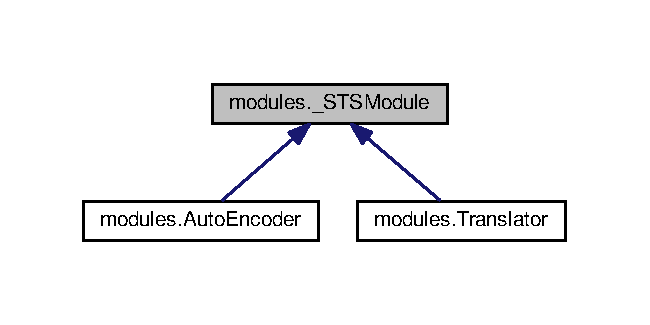
\includegraphics[width=312pt]{classmodules_1_1__STSModule__inherit__graph}
\end{center}
\end{figure}
\subsection*{Public Member Functions}
\begin{DoxyCompactItemize}
\item 
def {\bfseries \+\_\+\+\_\+init\+\_\+\+\_\+}\hypertarget{classmodules_1_1__STSModule_a634c7045b2702b3083efe93386d60d22}{}\label{classmodules_1_1__STSModule_a634c7045b2702b3083efe93386d60d22}

\item 
def {\bfseries model} (self)\hypertarget{classmodules_1_1__STSModule_a39d3e3d2d8bc1c5b5345c40629394834}{}\label{classmodules_1_1__STSModule_a39d3e3d2d8bc1c5b5345c40629394834}

\item 
def {\bfseries model} (self, model)\hypertarget{classmodules_1_1__STSModule_aeca7d7f6542570f382e6469723db1b04}{}\label{classmodules_1_1__STSModule_aeca7d7f6542570f382e6469723db1b04}

\end{DoxyCompactItemize}


\subsection{Detailed Description}
\begin{DoxyVerb}A base class for the sequence-to-sequence type modules.
\end{DoxyVerb}
 

The documentation for this class was generated from the following file\+:\begin{DoxyCompactItemize}
\item 
src/modules/modules.\+py\end{DoxyCompactItemize}

\hypertarget{classanalysis_1_1Analyzer}{}\section{analysis.\+Analyzer Class Reference}
\label{classanalysis_1_1Analyzer}\index{analysis.\+Analyzer@{analysis.\+Analyzer}}
\subsection*{Public Member Functions}
\begin{DoxyCompactItemize}
\item 
def {\bfseries \+\_\+\+\_\+init\+\_\+\+\_\+} (self, directory)\hypertarget{classanalysis_1_1Analyzer_a31ea6d2257834ac6334c9a2896b58e96}{}\label{classanalysis_1_1Analyzer_a31ea6d2257834ac6334c9a2896b58e96}

\item 
def {\bfseries show\+\_\+available\+\_\+metrics} (self)\hypertarget{classanalysis_1_1Analyzer_a694a48d9f544ee44dd8574479dad19bf}{}\label{classanalysis_1_1Analyzer_a694a48d9f544ee44dd8574479dad19bf}

\item 
def {\bfseries show\+\_\+validation\+\_\+identifiers} (self)\hypertarget{classanalysis_1_1Analyzer_a4026317b5faf8c89dcf4921c3ab3b630}{}\label{classanalysis_1_1Analyzer_a4026317b5faf8c89dcf4921c3ab3b630}

\item 
def {\bfseries display} (self, metric, mode, plot\+\_\+size=Plot.\+P\+L\+O\+T\+\_\+\+S\+I\+ZE, tokens=None, epoch\+\_\+range=(None,), identifiers=None, kwargs)\hypertarget{classanalysis_1_1Analyzer_a0d170e69cc1a1507411a665873d40cd1}{}\label{classanalysis_1_1Analyzer_a0d170e69cc1a1507411a665873d40cd1}

\end{DoxyCompactItemize}
\subsection*{Static Public Attributes}
\begin{DoxyCompactItemize}
\item 
string {\bfseries T\+E\+S\+T\+\_\+\+F\+I\+LE} = \textquotesingle{}test.\+pt\textquotesingle{}\hypertarget{classanalysis_1_1Analyzer_a5ba821b80838b7b94c7ed5e90f29f50d}{}\label{classanalysis_1_1Analyzer_a5ba821b80838b7b94c7ed5e90f29f50d}

\item 
string {\bfseries E\+V\+A\+L\+\_\+\+F\+I\+LE} = \textquotesingle{}eval.\+pt\textquotesingle{}\hypertarget{classanalysis_1_1Analyzer_a43467316054aac4a8431653aabc3048d}{}\label{classanalysis_1_1Analyzer_a43467316054aac4a8431653aabc3048d}

\item 
string {\bfseries O\+U\+T\+P\+U\+T\+\_\+\+D\+IR} = \textquotesingle{}outputs\textquotesingle{}\hypertarget{classanalysis_1_1Analyzer_ae639170ee9cec8f748c2b56f8e62b8ca}{}\label{classanalysis_1_1Analyzer_ae639170ee9cec8f748c2b56f8e62b8ca}

\item 
string {\bfseries T\+R\+A\+I\+N\+\_\+\+M\+O\+DE} = \textquotesingle{}train\textquotesingle{}\hypertarget{classanalysis_1_1Analyzer_a6d013c22abf2ccb3d3c54d88c5776a9c}{}\label{classanalysis_1_1Analyzer_a6d013c22abf2ccb3d3c54d88c5776a9c}

\item 
string {\bfseries V\+A\+L\+I\+D\+A\+T\+I\+O\+N\+\_\+\+M\+O\+DE} = \textquotesingle{}validation\textquotesingle{}\hypertarget{classanalysis_1_1Analyzer_a76be0f0e67007845576c35ddbe07db90}{}\label{classanalysis_1_1Analyzer_a76be0f0e67007845576c35ddbe07db90}

\item 
string {\bfseries T\+E\+S\+T\+\_\+\+M\+O\+DE} = \textquotesingle{}test\textquotesingle{}\hypertarget{classanalysis_1_1Analyzer_a67fe7bc673b4765058c728f4b57298da}{}\label{classanalysis_1_1Analyzer_a67fe7bc673b4765058c728f4b57298da}

\item 
string {\bfseries E\+V\+A\+L\+U\+A\+T\+I\+O\+N\+\_\+\+M\+O\+DE} = \textquotesingle{}evaluation\textquotesingle{}\hypertarget{classanalysis_1_1Analyzer_afc7581bdcfed5babeb60ba0859ef64ee}{}\label{classanalysis_1_1Analyzer_afc7581bdcfed5babeb60ba0859ef64ee}

\end{DoxyCompactItemize}


\subsection{Detailed Description}
\begin{DoxyVerb}\end{DoxyVerb}
 

The documentation for this class was generated from the following file\+:\begin{DoxyCompactItemize}
\item 
src/utils/analysis.\+py\end{DoxyCompactItemize}

\hypertarget{classanalysis_1_1AttentionData}{}\section{analysis.\+Attention\+Data Class Reference}
\label{classanalysis_1_1AttentionData}\index{analysis.\+Attention\+Data@{analysis.\+Attention\+Data}}


Inheritance diagram for analysis.\+Attention\+Data\+:
\nopagebreak
\begin{figure}[H]
\begin{center}
\leavevmode
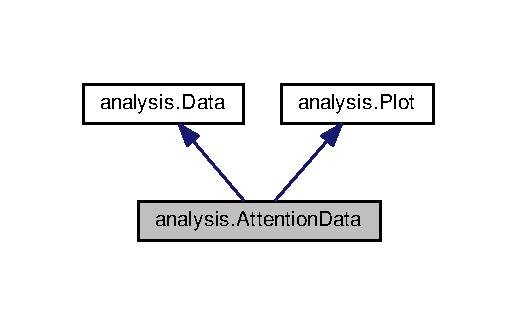
\includegraphics[width=248pt]{classanalysis_1_1AttentionData__inherit__graph}
\end{center}
\end{figure}


Collaboration diagram for analysis.\+Attention\+Data\+:
\nopagebreak
\begin{figure}[H]
\begin{center}
\leavevmode
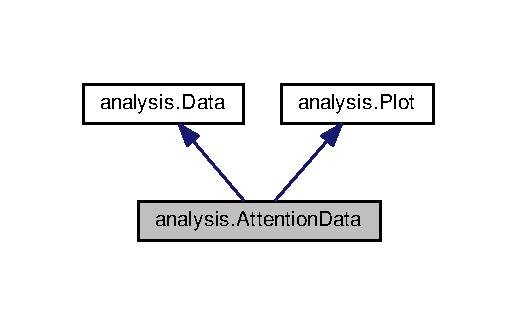
\includegraphics[width=248pt]{classanalysis_1_1AttentionData__coll__graph}
\end{center}
\end{figure}
\subsection*{Public Member Functions}
\begin{DoxyCompactItemize}
\item 
def {\bfseries \+\_\+\+\_\+init\+\_\+\+\_\+} (self)\hypertarget{classanalysis_1_1AttentionData_a5f53d61098b4771aea85433acd1b7bc4}{}\label{classanalysis_1_1AttentionData_a5f53d61098b4771aea85433acd1b7bc4}

\item 
def {\bfseries get\+\_\+required\+\_\+keys} (self)\hypertarget{classanalysis_1_1AttentionData_a0a9bf2709ad0a6be6d04ebc6f271d9fa}{}\label{classanalysis_1_1AttentionData_a0a9bf2709ad0a6be6d04ebc6f271d9fa}

\item 
def {\bfseries add} (self, identifier, value)\hypertarget{classanalysis_1_1AttentionData_a3140fc99e83d19bf7cb6c563330a51e1}{}\label{classanalysis_1_1AttentionData_a3140fc99e83d19bf7cb6c563330a51e1}

\end{DoxyCompactItemize}
\subsection*{Static Public Member Functions}
\begin{DoxyCompactItemize}
\item 
def {\bfseries display} (data, plot\+\_\+size, epochs, epoch\+\_\+range, identifiers=None, params)\hypertarget{classanalysis_1_1AttentionData_a18bd9c557c02f1edf07b928d37bbce40}{}\label{classanalysis_1_1AttentionData_a18bd9c557c02f1edf07b928d37bbce40}

\end{DoxyCompactItemize}
\subsection*{Additional Inherited Members}


\subsection{Detailed Description}
\begin{DoxyVerb}\end{DoxyVerb}
 

The documentation for this class was generated from the following file\+:\begin{DoxyCompactItemize}
\item 
src/utils/analysis.\+py\end{DoxyCompactItemize}

\hypertarget{classrnn_1_1AttentionRNNDecoder}{}\section{rnn.\+Attention\+R\+N\+N\+Decoder Class Reference}
\label{classrnn_1_1AttentionRNNDecoder}\index{rnn.\+Attention\+R\+N\+N\+Decoder@{rnn.\+Attention\+R\+N\+N\+Decoder}}


Inheritance diagram for rnn.\+Attention\+R\+N\+N\+Decoder\+:
\nopagebreak
\begin{figure}[H]
\begin{center}
\leavevmode
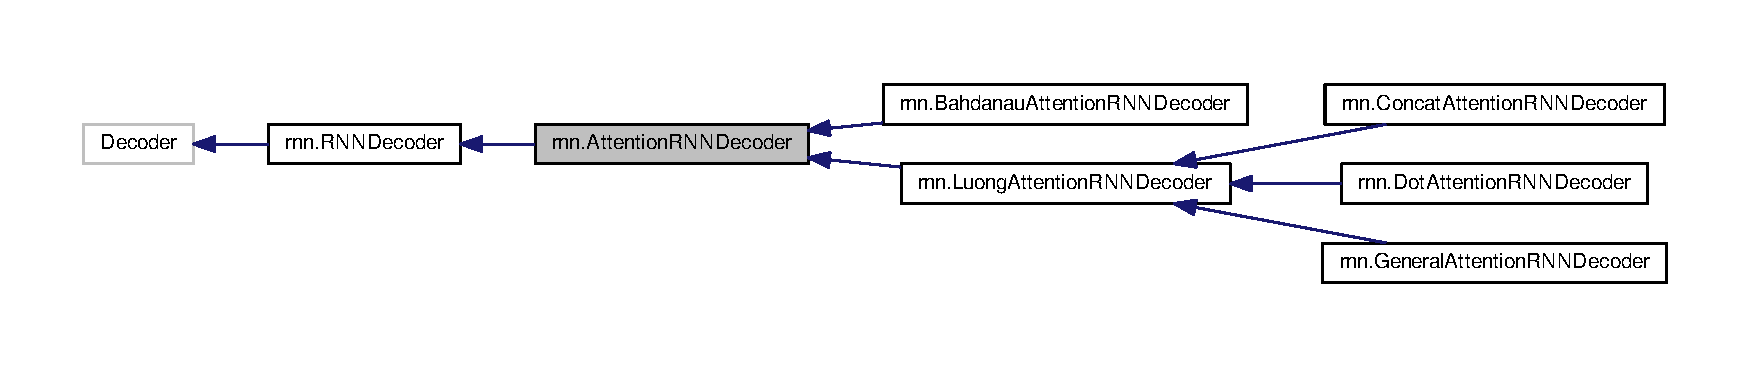
\includegraphics[width=350pt]{classrnn_1_1AttentionRNNDecoder__inherit__graph}
\end{center}
\end{figure}


Collaboration diagram for rnn.\+Attention\+R\+N\+N\+Decoder\+:
\nopagebreak
\begin{figure}[H]
\begin{center}
\leavevmode
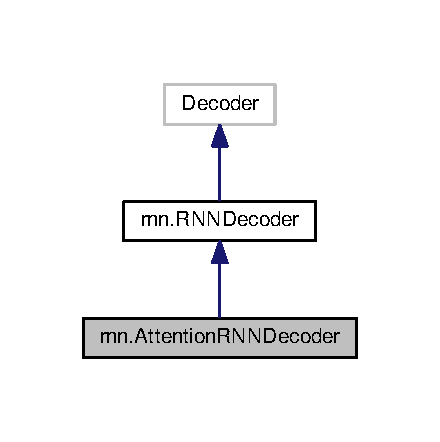
\includegraphics[width=211pt]{classrnn_1_1AttentionRNNDecoder__coll__graph}
\end{center}
\end{figure}
\subsection*{Public Member Functions}
\begin{DoxyCompactItemize}
\item 
def {\bfseries \+\_\+\+\_\+init\+\_\+\+\_\+}\hypertarget{classrnn_1_1AttentionRNNDecoder_ac2fb22b90774fc0992f0fe2d03d7d697}{}\label{classrnn_1_1AttentionRNNDecoder_ac2fb22b90774fc0992f0fe2d03d7d697}

\item 
def \hyperlink{classrnn_1_1AttentionRNNDecoder_acf4927f9addaae2bc2d38eb3aac7353c}{init\+\_\+optimizer} (self)
\item 
def {\bfseries forward}\hypertarget{classrnn_1_1AttentionRNNDecoder_a5a07d962dc51732608e938a971b7551f}{}\label{classrnn_1_1AttentionRNNDecoder_a5a07d962dc51732608e938a971b7551f}

\item 
def {\bfseries output\+\_\+types} (self)\hypertarget{classrnn_1_1AttentionRNNDecoder_acd3abbdba97810519ea7867560f588e1}{}\label{classrnn_1_1AttentionRNNDecoder_acd3abbdba97810519ea7867560f588e1}

\item 
def {\bfseries optimizers} (self)\hypertarget{classrnn_1_1AttentionRNNDecoder_a65dece144c9b3924da10f7df664ad895}{}\label{classrnn_1_1AttentionRNNDecoder_a65dece144c9b3924da10f7df664ad895}

\item 
def \hyperlink{classrnn_1_1AttentionRNNDecoder_a59c5e56f0ed9ae9b5f259fe7a4293843}{state} (self)
\item 
def {\bfseries state}\hypertarget{classrnn_1_1AttentionRNNDecoder_a66f5dd341d9bf182d1b6dabb74dda027}{}\label{classrnn_1_1AttentionRNNDecoder_a66f5dd341d9bf182d1b6dabb74dda027}

\end{DoxyCompactItemize}
\subsection*{Static Public Attributes}
\begin{DoxyCompactItemize}
\item 
bool {\bfseries abstract} = True\hypertarget{classrnn_1_1AttentionRNNDecoder_ae72e8e8842b1ff3cf42f0fa799c13db5}{}\label{classrnn_1_1AttentionRNNDecoder_ae72e8e8842b1ff3cf42f0fa799c13db5}

\end{DoxyCompactItemize}
\subsection*{Additional Inherited Members}


\subsection{Detailed Description}
\begin{DoxyVerb}Abstract base class for the attentional variation of recurrent decoder unit.
\end{DoxyVerb}
 

\subsection{Member Function Documentation}
\index{rnn\+::\+Attention\+R\+N\+N\+Decoder@{rnn\+::\+Attention\+R\+N\+N\+Decoder}!init\+\_\+optimizer@{init\+\_\+optimizer}}
\index{init\+\_\+optimizer@{init\+\_\+optimizer}!rnn\+::\+Attention\+R\+N\+N\+Decoder@{rnn\+::\+Attention\+R\+N\+N\+Decoder}}
\subsubsection[{\texorpdfstring{init\+\_\+optimizer(self)}{init_optimizer(self)}}]{\setlength{\rightskip}{0pt plus 5cm}def rnn.\+Attention\+R\+N\+N\+Decoder.\+init\+\_\+optimizer (
\begin{DoxyParamCaption}
\item[{}]{self, }
\item[{}]{Decoder}
\end{DoxyParamCaption}
)}\hypertarget{classrnn_1_1AttentionRNNDecoder_acf4927f9addaae2bc2d38eb3aac7353c}{}\label{classrnn_1_1AttentionRNNDecoder_acf4927f9addaae2bc2d38eb3aac7353c}
\begin{DoxyVerb}Initializes the optimizer for the decoder.
\end{DoxyVerb}
 \index{rnn\+::\+Attention\+R\+N\+N\+Decoder@{rnn\+::\+Attention\+R\+N\+N\+Decoder}!state@{state}}
\index{state@{state}!rnn\+::\+Attention\+R\+N\+N\+Decoder@{rnn\+::\+Attention\+R\+N\+N\+Decoder}}
\subsubsection[{\texorpdfstring{state(self)}{state(self)}}]{\setlength{\rightskip}{0pt plus 5cm}def rnn.\+Attention\+R\+N\+N\+Decoder.\+state (
\begin{DoxyParamCaption}
\item[{}]{self, }
\item[{}]{dict}
\end{DoxyParamCaption}
)}\hypertarget{classrnn_1_1AttentionRNNDecoder_a59c5e56f0ed9ae9b5f259fe7a4293843}{}\label{classrnn_1_1AttentionRNNDecoder_a59c5e56f0ed9ae9b5f259fe7a4293843}
\begin{DoxyVerb}Property for the optimizers of the decoder.
\end{DoxyVerb}
 

The documentation for this class was generated from the following file\+:\begin{DoxyCompactItemize}
\item 
src/components/decoders/rnn.\+py\end{DoxyCompactItemize}

\hypertarget{classmodules_1_1AutoEncoder}{}\section{modules.\+Auto\+Encoder Class Reference}
\label{classmodules_1_1AutoEncoder}\index{modules.\+Auto\+Encoder@{modules.\+Auto\+Encoder}}


Inheritance diagram for modules.\+Auto\+Encoder\+:
\nopagebreak
\begin{figure}[H]
\begin{center}
\leavevmode
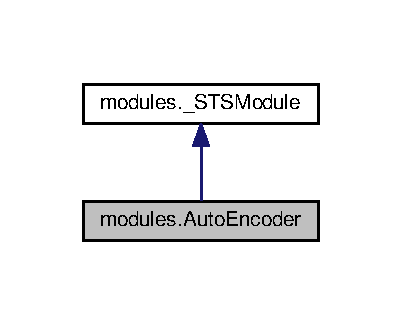
\includegraphics[width=193pt]{classmodules_1_1AutoEncoder__inherit__graph}
\end{center}
\end{figure}


Collaboration diagram for modules.\+Auto\+Encoder\+:
\nopagebreak
\begin{figure}[H]
\begin{center}
\leavevmode
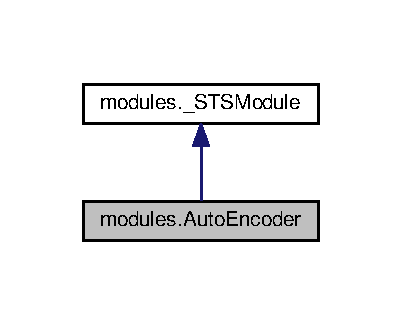
\includegraphics[width=193pt]{classmodules_1_1AutoEncoder__coll__graph}
\end{center}
\end{figure}
\subsection*{Public Member Functions}
\begin{DoxyCompactItemize}
\item 
def {\bfseries \+\_\+\+\_\+init\+\_\+\+\_\+}\hypertarget{classmodules_1_1AutoEncoder_ab330fa1ddf4e6749656099ed1d5b3881}{}\label{classmodules_1_1AutoEncoder_ab330fa1ddf4e6749656099ed1d5b3881}

\item 
def {\bfseries \+\_\+\+\_\+call\+\_\+\+\_\+}\hypertarget{classmodules_1_1AutoEncoder_a631368683346bf1ce00569e76dfbeeab}{}\label{classmodules_1_1AutoEncoder_a631368683346bf1ce00569e76dfbeeab}

\end{DoxyCompactItemize}


\subsection{Detailed Description}
\begin{DoxyVerb}Auto-encoder module for a sequence-to-sequence type model.
\end{DoxyVerb}
 

The documentation for this class was generated from the following file\+:\begin{DoxyCompactItemize}
\item 
src/modules/modules.\+py\end{DoxyCompactItemize}

\hypertarget{classrnn_1_1BahdanauAttentionRNNDecoder}{}\section{rnn.\+Bahdanau\+Attention\+R\+N\+N\+Decoder Class Reference}
\label{classrnn_1_1BahdanauAttentionRNNDecoder}\index{rnn.\+Bahdanau\+Attention\+R\+N\+N\+Decoder@{rnn.\+Bahdanau\+Attention\+R\+N\+N\+Decoder}}


Inheritance diagram for rnn.\+Bahdanau\+Attention\+R\+N\+N\+Decoder\+:
\nopagebreak
\begin{figure}[H]
\begin{center}
\leavevmode
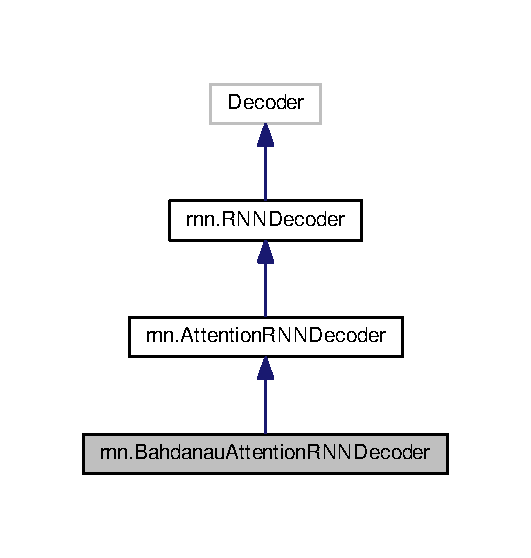
\includegraphics[width=255pt]{classrnn_1_1BahdanauAttentionRNNDecoder__inherit__graph}
\end{center}
\end{figure}


Collaboration diagram for rnn.\+Bahdanau\+Attention\+R\+N\+N\+Decoder\+:
\nopagebreak
\begin{figure}[H]
\begin{center}
\leavevmode
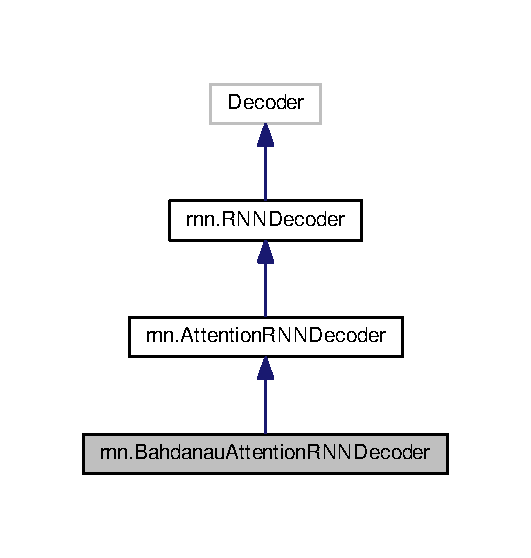
\includegraphics[width=255pt]{classrnn_1_1BahdanauAttentionRNNDecoder__coll__graph}
\end{center}
\end{figure}
\subsection*{Public Member Functions}
\begin{DoxyCompactItemize}
\item 
def {\bfseries \+\_\+\+\_\+init\+\_\+\+\_\+}\hypertarget{classrnn_1_1BahdanauAttentionRNNDecoder_a0c718fa50c4707dc06ed5612aec9ae8a}{}\label{classrnn_1_1BahdanauAttentionRNNDecoder_a0c718fa50c4707dc06ed5612aec9ae8a}

\item 
def \hyperlink{classrnn_1_1BahdanauAttentionRNNDecoder_af01d308f26b7f7ae728c1df16cbe574a}{init\+\_\+parameters} (self)
\end{DoxyCompactItemize}
\subsection*{Static Public Attributes}
\begin{DoxyCompactItemize}
\item 
{\bfseries interface}
\item 
bool {\bfseries abstract} = False\hypertarget{classrnn_1_1BahdanauAttentionRNNDecoder_addf7d4bd064d2f44da26829091293820}{}\label{classrnn_1_1BahdanauAttentionRNNDecoder_addf7d4bd064d2f44da26829091293820}

\end{DoxyCompactItemize}
\subsection*{Additional Inherited Members}


\subsection{Detailed Description}
\begin{DoxyVerb}Global attention mechanism for the recurrent decoder module. The algorithm is based on:

    https://arxiv.org/pdf/1409.0473.pdf

The computational path of the method differs from the Luong style, since
the context vector contributes to the calculation of the hidden state as well, created
by the recurrent unit at time step t.

    h(t-1) -> a(t) -> c(t) -> h(t)

The attention weights are derived from the similarity scores of the previous recurrent hidden
state (from time step t-1) and the encoder outputs. The created context vector is then merged with
the output of the recurrent unit as well, to get the final output of a softmax layer, providing the
probability distribution over the word ids.
\end{DoxyVerb}
 

\subsection{Member Function Documentation}
\index{rnn\+::\+Bahdanau\+Attention\+R\+N\+N\+Decoder@{rnn\+::\+Bahdanau\+Attention\+R\+N\+N\+Decoder}!init\+\_\+parameters@{init\+\_\+parameters}}
\index{init\+\_\+parameters@{init\+\_\+parameters}!rnn\+::\+Bahdanau\+Attention\+R\+N\+N\+Decoder@{rnn\+::\+Bahdanau\+Attention\+R\+N\+N\+Decoder}}
\subsubsection[{\texorpdfstring{init\+\_\+parameters(self)}{init_parameters(self)}}]{\setlength{\rightskip}{0pt plus 5cm}def rnn.\+Bahdanau\+Attention\+R\+N\+N\+Decoder.\+init\+\_\+parameters (
\begin{DoxyParamCaption}
\item[{}]{self, }
\item[{}]{Decoder}
\end{DoxyParamCaption}
)}\hypertarget{classrnn_1_1BahdanauAttentionRNNDecoder_af01d308f26b7f7ae728c1df16cbe574a}{}\label{classrnn_1_1BahdanauAttentionRNNDecoder_af01d308f26b7f7ae728c1df16cbe574a}
\begin{DoxyVerb}Initializes the parameters for the decoder.
\end{DoxyVerb}
 

\subsection{Member Data Documentation}
\index{rnn\+::\+Bahdanau\+Attention\+R\+N\+N\+Decoder@{rnn\+::\+Bahdanau\+Attention\+R\+N\+N\+Decoder}!interface@{interface}}
\index{interface@{interface}!rnn\+::\+Bahdanau\+Attention\+R\+N\+N\+Decoder@{rnn\+::\+Bahdanau\+Attention\+R\+N\+N\+Decoder}}
\subsubsection[{\texorpdfstring{interface}{interface}}]{\setlength{\rightskip}{0pt plus 5cm}rnn.\+Bahdanau\+Attention\+R\+N\+N\+Decoder.\+interface\hspace{0.3cm}{\ttfamily [static]}}\hypertarget{classrnn_1_1BahdanauAttentionRNNDecoder_ac0c8ea546f7e3bf096e8e5815a887c80}{}\label{classrnn_1_1BahdanauAttentionRNNDecoder_ac0c8ea546f7e3bf096e8e5815a887c80}
{\bfseries Initial value\+:}
\begin{DoxyCode}
1 = Interface(**\{
2         **subtract\_dict(RNNDecoder.interface.dictionary, \{\textcolor{stringliteral}{'input\_size'}: \textcolor{keywordtype}{None}\}),
3         \textcolor{stringliteral}{'input\_size'}: (Interface.last\_key(subtract\_dict(RNNDecoder.interface.dictionary, \{\textcolor{stringliteral}{'input\_size'}: \textcolor{keywordtype}{
      None}\})) + 1,
4                        \textcolor{stringliteral}{'Decoder:embedding\_size$ + Decoder:hidden\_size$'})
5     \})
\end{DoxyCode}


The documentation for this class was generated from the following file\+:\begin{DoxyCompactItemize}
\item 
src/components/decoders/rnn.\+py\end{DoxyCompactItemize}

\hypertarget{classrnn_1_1BidirectionalRNNEncoder}{}\section{rnn.\+Bidirectional\+R\+N\+N\+Encoder Class Reference}
\label{classrnn_1_1BidirectionalRNNEncoder}\index{rnn.\+Bidirectional\+R\+N\+N\+Encoder@{rnn.\+Bidirectional\+R\+N\+N\+Encoder}}


Inheritance diagram for rnn.\+Bidirectional\+R\+N\+N\+Encoder\+:
\nopagebreak
\begin{figure}[H]
\begin{center}
\leavevmode
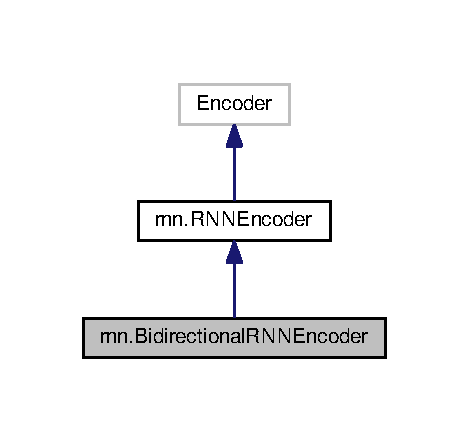
\includegraphics[width=225pt]{classrnn_1_1BidirectionalRNNEncoder__inherit__graph}
\end{center}
\end{figure}


Collaboration diagram for rnn.\+Bidirectional\+R\+N\+N\+Encoder\+:
\nopagebreak
\begin{figure}[H]
\begin{center}
\leavevmode
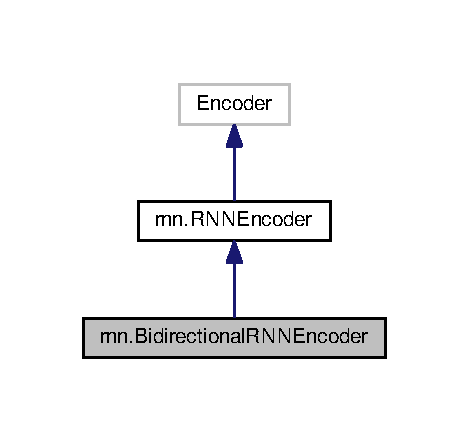
\includegraphics[width=225pt]{classrnn_1_1BidirectionalRNNEncoder__coll__graph}
\end{center}
\end{figure}
\subsection*{Public Member Functions}
\begin{DoxyCompactItemize}
\item 
def {\bfseries \+\_\+\+\_\+init\+\_\+\+\_\+} (self, parameter\+\_\+setter)\hypertarget{classrnn_1_1BidirectionalRNNEncoder_acf8de7a3fa694e7f17c129472db6beca}{}\label{classrnn_1_1BidirectionalRNNEncoder_acf8de7a3fa694e7f17c129472db6beca}

\item 
def \hyperlink{classrnn_1_1BidirectionalRNNEncoder_a038860b36d2869ad536345ba054e8cee}{init\+\_\+parameters} (self)
\item 
def \hyperlink{classrnn_1_1BidirectionalRNNEncoder_a32673b75f9536ce891018073f6467fd4}{forward} (self, inputs, lengths)
\end{DoxyCompactItemize}
\subsection*{Static Public Attributes}
\begin{DoxyCompactItemize}
\item 
{\bfseries interface} = R\+N\+N\+Encoder.\+interface\hypertarget{classrnn_1_1BidirectionalRNNEncoder_aad07c0c8c5211291502c242263f8f766}{}\label{classrnn_1_1BidirectionalRNNEncoder_aad07c0c8c5211291502c242263f8f766}

\item 
bool {\bfseries abstract} = False\hypertarget{classrnn_1_1BidirectionalRNNEncoder_a58c145d0b71eb6bf19517e51965599f0}{}\label{classrnn_1_1BidirectionalRNNEncoder_a58c145d0b71eb6bf19517e51965599f0}

\end{DoxyCompactItemize}
\subsection*{Additional Inherited Members}


\subsection{Detailed Description}
\begin{DoxyVerb}\end{DoxyVerb}
 

\subsection{Member Function Documentation}
\index{rnn\+::\+Bidirectional\+R\+N\+N\+Encoder@{rnn\+::\+Bidirectional\+R\+N\+N\+Encoder}!forward@{forward}}
\index{forward@{forward}!rnn\+::\+Bidirectional\+R\+N\+N\+Encoder@{rnn\+::\+Bidirectional\+R\+N\+N\+Encoder}}
\subsubsection[{\texorpdfstring{forward(self, inputs, lengths)}{forward(self, inputs, lengths)}}]{\setlength{\rightskip}{0pt plus 5cm}def rnn.\+Bidirectional\+R\+N\+N\+Encoder.\+forward (
\begin{DoxyParamCaption}
\item[{}]{self, }
\item[{}]{inputs, }
\item[{}]{lengths}
\end{DoxyParamCaption}
)}\hypertarget{classrnn_1_1BidirectionalRNNEncoder_a32673b75f9536ce891018073f6467fd4}{}\label{classrnn_1_1BidirectionalRNNEncoder_a32673b75f9536ce891018073f6467fd4}
\begin{DoxyVerb}A forward step of the encoder. The batch of sequences with word ids are
packed into padded_sequence object, which are processed by the recurrent layer.

:param inputs:
    Variable, (batch_size, sequence_length) containing the ids of the words.

:param lengths:
    Ndarray, containing the real lengths of the sequences in the batch (prior to padding).

:return outputs:
    Variable, (batch_size, sequence_length, vocab_size) the output at each time
    step of the encoder.

:return hidden_state:
    Variable, (num_layers * directions, batch_size, hidden_size) the final hidden state.
\end{DoxyVerb}
 \index{rnn\+::\+Bidirectional\+R\+N\+N\+Encoder@{rnn\+::\+Bidirectional\+R\+N\+N\+Encoder}!init\+\_\+parameters@{init\+\_\+parameters}}
\index{init\+\_\+parameters@{init\+\_\+parameters}!rnn\+::\+Bidirectional\+R\+N\+N\+Encoder@{rnn\+::\+Bidirectional\+R\+N\+N\+Encoder}}
\subsubsection[{\texorpdfstring{init\+\_\+parameters(self)}{init_parameters(self)}}]{\setlength{\rightskip}{0pt plus 5cm}def rnn.\+Bidirectional\+R\+N\+N\+Encoder.\+init\+\_\+parameters (
\begin{DoxyParamCaption}
\item[{}]{self}
\end{DoxyParamCaption}
)}\hypertarget{classrnn_1_1BidirectionalRNNEncoder_a038860b36d2869ad536345ba054e8cee}{}\label{classrnn_1_1BidirectionalRNNEncoder_a038860b36d2869ad536345ba054e8cee}
\begin{DoxyVerb}Calls the parameter setter, which initializes the Parameter type attributes.
After initialization, the main components of the encoder, which require the previously
initialized parameter values, are created as well.
\end{DoxyVerb}
 

The documentation for this class was generated from the following file\+:\begin{DoxyCompactItemize}
\item 
src/components/encoders/rnn.\+py\end{DoxyCompactItemize}

\hypertarget{classreader_1_1Bilingual}{}\section{reader.\+Bilingual Class Reference}
\label{classreader_1_1Bilingual}\index{reader.\+Bilingual@{reader.\+Bilingual}}


Inheritance diagram for reader.\+Bilingual\+:
\nopagebreak
\begin{figure}[H]
\begin{center}
\leavevmode
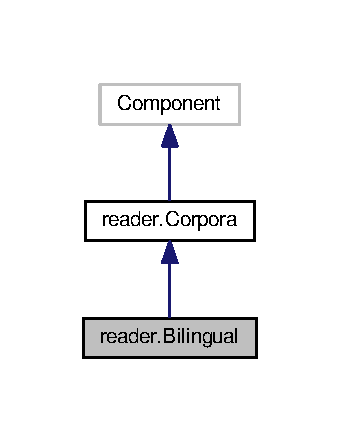
\includegraphics[width=163pt]{classreader_1_1Bilingual__inherit__graph}
\end{center}
\end{figure}


Collaboration diagram for reader.\+Bilingual\+:
\nopagebreak
\begin{figure}[H]
\begin{center}
\leavevmode
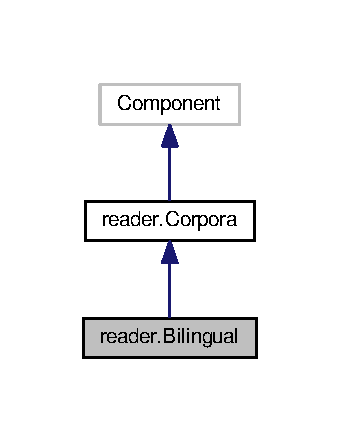
\includegraphics[width=163pt]{classreader_1_1Bilingual__coll__graph}
\end{center}
\end{figure}
\subsection*{Additional Inherited Members}


The documentation for this class was generated from the following file\+:\begin{DoxyCompactItemize}
\item 
src/utils/reader.\+py\end{DoxyCompactItemize}

\hypertarget{classutils_1_1Classifier}{}\section{utils.\+Classifier Class Reference}
\label{classutils_1_1Classifier}\index{utils.\+Classifier@{utils.\+Classifier}}


Inheritance diagram for utils.\+Classifier\+:
\nopagebreak
\begin{figure}[H]
\begin{center}
\leavevmode
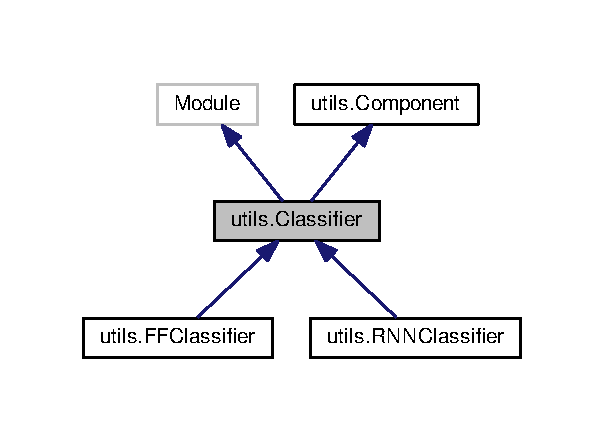
\includegraphics[width=290pt]{classutils_1_1Classifier__inherit__graph}
\end{center}
\end{figure}


Collaboration diagram for utils.\+Classifier\+:
\nopagebreak
\begin{figure}[H]
\begin{center}
\leavevmode
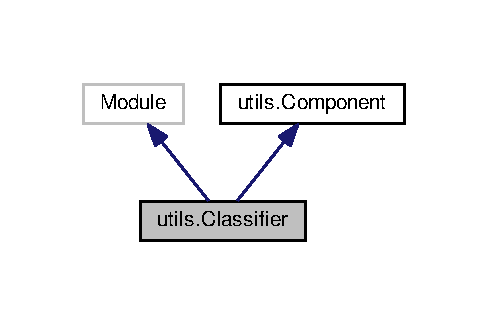
\includegraphics[width=234pt]{classutils_1_1Classifier__coll__graph}
\end{center}
\end{figure}
\subsection*{Public Member Functions}
\begin{DoxyCompactItemize}
\item 
def {\bfseries \+\_\+\+\_\+init\+\_\+\+\_\+}\hypertarget{classutils_1_1Classifier_af4e343de12b5e4bbdc597bf83e09e074}{}\label{classutils_1_1Classifier_af4e343de12b5e4bbdc597bf83e09e074}

\item 
def {\bfseries forward} (self, args, kwargs)\hypertarget{classutils_1_1Classifier_ac953237bb39ddf21b4c4417704acbdb3}{}\label{classutils_1_1Classifier_ac953237bb39ddf21b4c4417704acbdb3}

\item 
def {\bfseries optimizer} (self)\hypertarget{classutils_1_1Classifier_a38fc9590b1eee361c3649e49b99905a8}{}\label{classutils_1_1Classifier_a38fc9590b1eee361c3649e49b99905a8}

\item 
def {\bfseries freeze} (self)\hypertarget{classutils_1_1Classifier_a77f6d76d07a2ee3cff6f80b4191865b2}{}\label{classutils_1_1Classifier_a77f6d76d07a2ee3cff6f80b4191865b2}

\item 
def {\bfseries unfreeze} (self)\hypertarget{classutils_1_1Classifier_a2c8049a8b7af725e0905e6228a7508e3}{}\label{classutils_1_1Classifier_a2c8049a8b7af725e0905e6228a7508e3}

\end{DoxyCompactItemize}
\subsection*{Static Public Attributes}
\begin{DoxyCompactItemize}
\item 
{\bfseries interface}
\end{DoxyCompactItemize}


\subsection{Detailed Description}
\begin{DoxyVerb}Abstract base class for the discriminator modules, mainly used for the unsupervised
translation task. Any newly added discriminator type module must inherit from this
super class, otherwise it won't be discoverable by the hierarchy builder utility.
\end{DoxyVerb}
 

\subsection{Member Data Documentation}
\index{utils\+::\+Classifier@{utils\+::\+Classifier}!interface@{interface}}
\index{interface@{interface}!utils\+::\+Classifier@{utils\+::\+Classifier}}
\subsubsection[{\texorpdfstring{interface}{interface}}]{\setlength{\rightskip}{0pt plus 5cm}utils.\+Classifier.\+interface\hspace{0.3cm}{\ttfamily [static]}}\hypertarget{classutils_1_1Classifier_ab68dd332ac9c3c4117cccccca9c77220}{}\label{classutils_1_1Classifier_ab68dd332ac9c3c4117cccccca9c77220}
{\bfseries Initial value\+:}
\begin{DoxyCode}
1 = Interface(**\{
2         \textcolor{stringliteral}{'hidden\_size'}:      (0, \textcolor{keywordtype}{None}),
3         \textcolor{stringliteral}{'learning\_rate'}:    (1, \textcolor{keywordtype}{None}),
4         \textcolor{stringliteral}{'optimizer\_type'}:   (2, \textcolor{keywordtype}{None}),
5         \textcolor{stringliteral}{'output\_size'}:      (3, \textcolor{keywordtype}{None}),
6         \textcolor{stringliteral}{'cuda'}:             (4, \textcolor{stringliteral}{'Experiment:Policy:cuda$'}),
7         \textcolor{stringliteral}{'input\_size'}:       (5, \textcolor{stringliteral}{'Encoder:hidden\_size$'})
8     \})
\end{DoxyCode}


The documentation for this class was generated from the following file\+:\begin{DoxyCompactItemize}
\item 
src/components/utils/utils.\+py\end{DoxyCompactItemize}

\hypertarget{classcnn_1_1CNNDecoder}{}\section{cnn.\+C\+N\+N\+Decoder Class Reference}
\label{classcnn_1_1CNNDecoder}\index{cnn.\+C\+N\+N\+Decoder@{cnn.\+C\+N\+N\+Decoder}}


Inheritance diagram for cnn.\+C\+N\+N\+Decoder\+:
\nopagebreak
\begin{figure}[H]
\begin{center}
\leavevmode
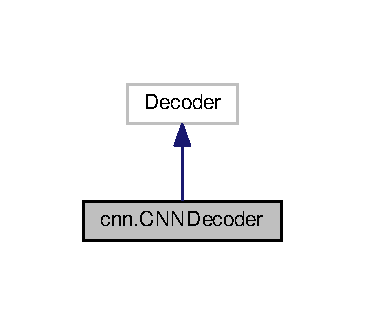
\includegraphics[width=175pt]{classcnn_1_1CNNDecoder__inherit__graph}
\end{center}
\end{figure}


Collaboration diagram for cnn.\+C\+N\+N\+Decoder\+:
\nopagebreak
\begin{figure}[H]
\begin{center}
\leavevmode
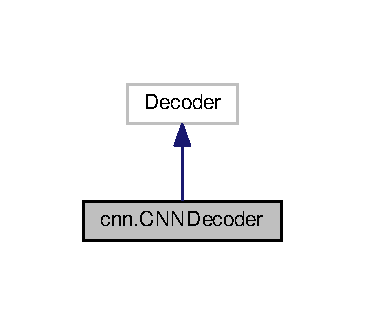
\includegraphics[width=175pt]{classcnn_1_1CNNDecoder__coll__graph}
\end{center}
\end{figure}


The documentation for this class was generated from the following file\+:\begin{DoxyCompactItemize}
\item 
src/components/decoders/cnn.\+py\end{DoxyCompactItemize}

\hypertarget{classcnn_1_1CNNEncoder}{}\section{cnn.\+C\+N\+N\+Encoder Class Reference}
\label{classcnn_1_1CNNEncoder}\index{cnn.\+C\+N\+N\+Encoder@{cnn.\+C\+N\+N\+Encoder}}


Inheritance diagram for cnn.\+C\+N\+N\+Encoder\+:
\nopagebreak
\begin{figure}[H]
\begin{center}
\leavevmode
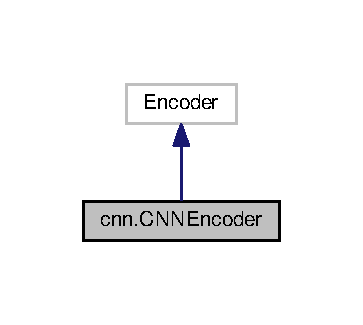
\includegraphics[width=174pt]{classcnn_1_1CNNEncoder__inherit__graph}
\end{center}
\end{figure}


Collaboration diagram for cnn.\+C\+N\+N\+Encoder\+:
\nopagebreak
\begin{figure}[H]
\begin{center}
\leavevmode
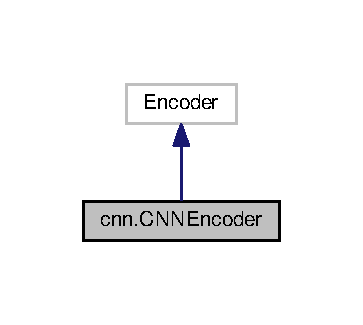
\includegraphics[width=174pt]{classcnn_1_1CNNEncoder__coll__graph}
\end{center}
\end{figure}


The documentation for this class was generated from the following file\+:\begin{DoxyCompactItemize}
\item 
src/components/encoders/cnn.\+py\end{DoxyCompactItemize}

\hypertarget{classutils_1_1Component}{}\section{utils.\+Component Class Reference}
\label{classutils_1_1Component}\index{utils.\+Component@{utils.\+Component}}


Inheritance diagram for utils.\+Component\+:
\nopagebreak
\begin{figure}[H]
\begin{center}
\leavevmode
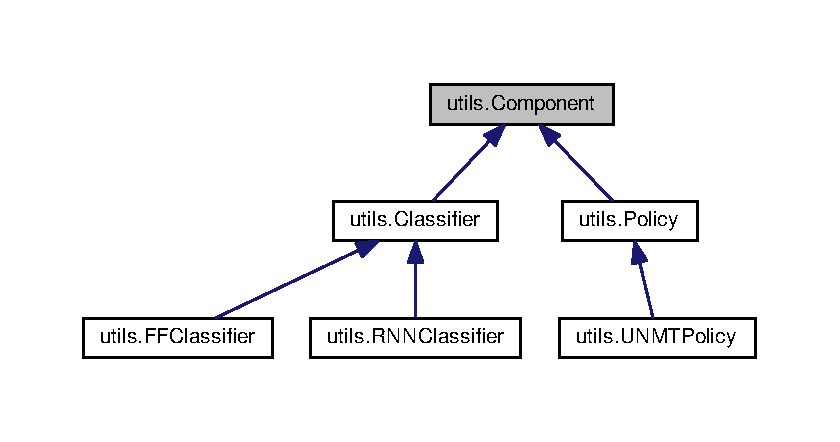
\includegraphics[width=350pt]{classutils_1_1Component__inherit__graph}
\end{center}
\end{figure}
\subsection*{Public Member Functions}
\begin{DoxyCompactItemize}
\item 
def \hyperlink{classutils_1_1Component_a09cbf7ace9815dc5e5595a35d5912f63}{properties} (self)
\end{DoxyCompactItemize}
\subsection*{Static Public Attributes}
\begin{DoxyCompactItemize}
\item 
{\bfseries interface} = None\hypertarget{classutils_1_1Component_a2329a886ae5a082efb0118b3e938249b}{}\label{classutils_1_1Component_a2329a886ae5a082efb0118b3e938249b}

\item 
bool {\bfseries abstract} = True\hypertarget{classutils_1_1Component_abb9cba8b93872c7cd890f49a0cda4619}{}\label{classutils_1_1Component_abb9cba8b93872c7cd890f49a0cda4619}

\end{DoxyCompactItemize}


\subsection{Detailed Description}
\begin{DoxyVerb}The base class for the components of the API.
\end{DoxyVerb}
 

\subsection{Member Function Documentation}
\index{utils\+::\+Component@{utils\+::\+Component}!properties@{properties}}
\index{properties@{properties}!utils\+::\+Component@{utils\+::\+Component}}
\subsubsection[{\texorpdfstring{properties(self)}{properties(self)}}]{\setlength{\rightskip}{0pt plus 5cm}def utils.\+Component.\+properties (
\begin{DoxyParamCaption}
\item[{}]{self}
\end{DoxyParamCaption}
)}\hypertarget{classutils_1_1Component_a09cbf7ace9815dc5e5595a35d5912f63}{}\label{classutils_1_1Component_a09cbf7ace9815dc5e5595a35d5912f63}
\begin{DoxyVerb}Convenience function for retrieving the properties of an instances, with their values.
\end{DoxyVerb}
 

The documentation for this class was generated from the following file\+:\begin{DoxyCompactItemize}
\item 
src/utils/utils.\+py\end{DoxyCompactItemize}

\hypertarget{classrnn_1_1ConcatAttentionRNNDecoder}{}\section{rnn.\+Concat\+Attention\+R\+N\+N\+Decoder Class Reference}
\label{classrnn_1_1ConcatAttentionRNNDecoder}\index{rnn.\+Concat\+Attention\+R\+N\+N\+Decoder@{rnn.\+Concat\+Attention\+R\+N\+N\+Decoder}}


Inheritance diagram for rnn.\+Concat\+Attention\+R\+N\+N\+Decoder\+:
\nopagebreak
\begin{figure}[H]
\begin{center}
\leavevmode
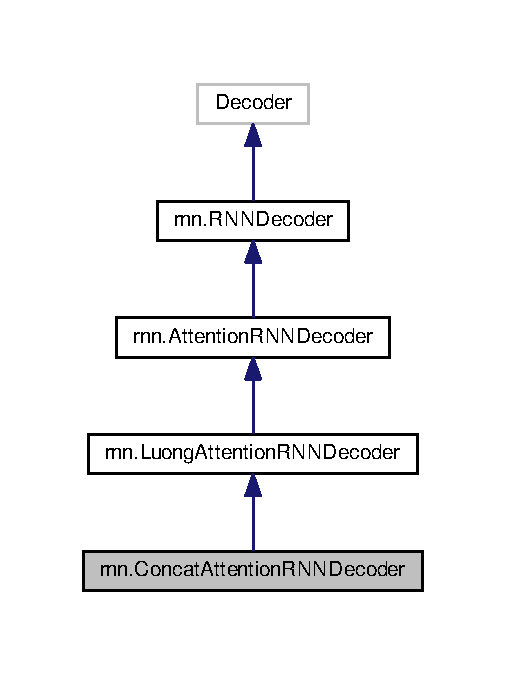
\includegraphics[width=243pt]{classrnn_1_1ConcatAttentionRNNDecoder__inherit__graph}
\end{center}
\end{figure}


Collaboration diagram for rnn.\+Concat\+Attention\+R\+N\+N\+Decoder\+:
\nopagebreak
\begin{figure}[H]
\begin{center}
\leavevmode
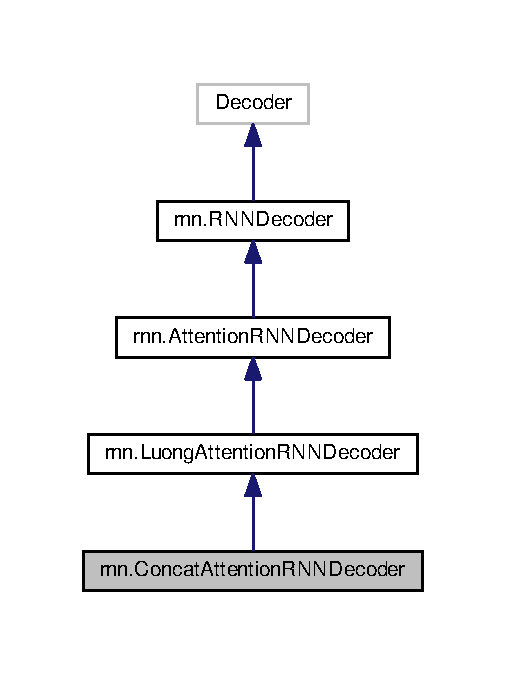
\includegraphics[width=243pt]{classrnn_1_1ConcatAttentionRNNDecoder__coll__graph}
\end{center}
\end{figure}
\subsection*{Public Member Functions}
\begin{DoxyCompactItemize}
\item 
def {\bfseries \+\_\+\+\_\+init\+\_\+\+\_\+}\hypertarget{classrnn_1_1ConcatAttentionRNNDecoder_aeac71794a63879580d75c06622c54194}{}\label{classrnn_1_1ConcatAttentionRNNDecoder_aeac71794a63879580d75c06622c54194}

\item 
def \hyperlink{classrnn_1_1ConcatAttentionRNNDecoder_ac69bf078fd13962611eecf184ae8a6bc}{init\+\_\+parameters} (self)
\end{DoxyCompactItemize}
\subsection*{Static Public Attributes}
\begin{DoxyCompactItemize}
\item 
{\bfseries interface} = R\+N\+N\+Decoder.\+interface\hypertarget{classrnn_1_1ConcatAttentionRNNDecoder_adb33ad797040b58dcb38bf8bd62437d1}{}\label{classrnn_1_1ConcatAttentionRNNDecoder_adb33ad797040b58dcb38bf8bd62437d1}

\item 
bool {\bfseries abstract} = False\hypertarget{classrnn_1_1ConcatAttentionRNNDecoder_a02c21a92b263ee91427642efa4b63699}{}\label{classrnn_1_1ConcatAttentionRNNDecoder_a02c21a92b263ee91427642efa4b63699}

\end{DoxyCompactItemize}
\subsection*{Additional Inherited Members}


\subsection{Detailed Description}
\begin{DoxyVerb}Global attention mechanism for the recurrent decoder module. The algorithm is a specific case
of Luong style attention, where the scoring is based off of the concatenation of the encoder
and decoder states, which is then passed through a non-linear layer with tanh activation.
The result is then multiplied by a vector to transform the final result to the correct size.
The scoring of similarity between encoder and decoder states is essentially the same as Bahdanau's
method, however the computation path follows the Luong style.
\end{DoxyVerb}
 

\subsection{Member Function Documentation}
\index{rnn\+::\+Concat\+Attention\+R\+N\+N\+Decoder@{rnn\+::\+Concat\+Attention\+R\+N\+N\+Decoder}!init\+\_\+parameters@{init\+\_\+parameters}}
\index{init\+\_\+parameters@{init\+\_\+parameters}!rnn\+::\+Concat\+Attention\+R\+N\+N\+Decoder@{rnn\+::\+Concat\+Attention\+R\+N\+N\+Decoder}}
\subsubsection[{\texorpdfstring{init\+\_\+parameters(self)}{init_parameters(self)}}]{\setlength{\rightskip}{0pt plus 5cm}def rnn.\+Concat\+Attention\+R\+N\+N\+Decoder.\+init\+\_\+parameters (
\begin{DoxyParamCaption}
\item[{}]{self, }
\item[{}]{Decoder}
\end{DoxyParamCaption}
)}\hypertarget{classrnn_1_1ConcatAttentionRNNDecoder_ac69bf078fd13962611eecf184ae8a6bc}{}\label{classrnn_1_1ConcatAttentionRNNDecoder_ac69bf078fd13962611eecf184ae8a6bc}
\begin{DoxyVerb}Initializes the parameters for the decoder.
\end{DoxyVerb}
 

The documentation for this class was generated from the following file\+:\begin{DoxyCompactItemize}
\item 
src/components/decoders/rnn.\+py\end{DoxyCompactItemize}

\hypertarget{classconfig_1_1Config}{}\section{config.\+Config Class Reference}
\label{classconfig_1_1Config}\index{config.\+Config@{config.\+Config}}
\subsection*{Public Member Functions}
\begin{DoxyCompactItemize}
\item 
def {\bfseries \+\_\+\+\_\+init\+\_\+\+\_\+}\hypertarget{classconfig_1_1Config_a2c77f4b64c0bf70b283cdb4af4c93fa1}{}\label{classconfig_1_1Config_a2c77f4b64c0bf70b283cdb4af4c93fa1}

\item 
def \hyperlink{classconfig_1_1Config_a4eaf8d72011aefb5237cd29bdbf659b3}{assemble} (self)
\end{DoxyCompactItemize}


\subsection{Detailed Description}
\begin{DoxyVerb}Class for handling configurations of models and tasks.
The configs are defined in JSON format files, which are parsed,
and instantiated with the help of interface definitions of the components.
Each node of the JSON file, that has a 'type' and 'params' key are Component type
objects.
\end{DoxyVerb}
 

\subsection{Member Function Documentation}
\index{config\+::\+Config@{config\+::\+Config}!assemble@{assemble}}
\index{assemble@{assemble}!config\+::\+Config@{config\+::\+Config}}
\subsubsection[{\texorpdfstring{assemble(self)}{assemble(self)}}]{\setlength{\rightskip}{0pt plus 5cm}def config.\+Config.\+assemble (
\begin{DoxyParamCaption}
\item[{}]{self, }
\item[{}]{tuple}
\end{DoxyParamCaption}
)}\hypertarget{classconfig_1_1Config_a4eaf8d72011aefb5237cd29bdbf659b3}{}\label{classconfig_1_1Config_a4eaf8d72011aefb5237cd29bdbf659b3}
\begin{DoxyVerb}Assembles the components, described by the interface of the task from the configuration file.

:return experiment:
    The initialized experiment object.

:return model_dir:
    The location of the experiment outputs.
\end{DoxyVerb}
 

The documentation for this class was generated from the following file\+:\begin{DoxyCompactItemize}
\item 
src/utils/config.\+py\end{DoxyCompactItemize}

\hypertarget{classreader_1_1Corpora}{}\section{reader.\+Corpora Class Reference}
\label{classreader_1_1Corpora}\index{reader.\+Corpora@{reader.\+Corpora}}


Inheritance diagram for reader.\+Corpora\+:
\nopagebreak
\begin{figure}[H]
\begin{center}
\leavevmode
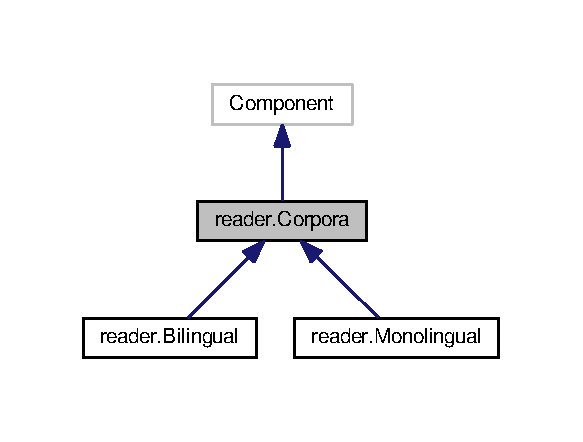
\includegraphics[width=280pt]{classreader_1_1Corpora__inherit__graph}
\end{center}
\end{figure}


Collaboration diagram for reader.\+Corpora\+:
\nopagebreak
\begin{figure}[H]
\begin{center}
\leavevmode
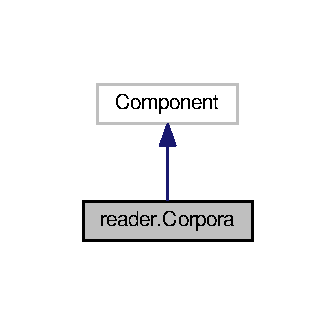
\includegraphics[width=161pt]{classreader_1_1Corpora__coll__graph}
\end{center}
\end{figure}
\subsection*{Public Member Functions}
\begin{DoxyCompactItemize}
\item 
def {\bfseries \+\_\+\+\_\+init\+\_\+\+\_\+}\hypertarget{classreader_1_1Corpora_a9ad3ac921ea96dc7f8fa8bf7c7ff229e}{}\label{classreader_1_1Corpora_a9ad3ac921ea96dc7f8fa8bf7c7ff229e}

\item 
def {\bfseries initialize\+\_\+corpus} (self)\hypertarget{classreader_1_1Corpora_aefb3138ee5f779ce6d2c59bcfd6c2036}{}\label{classreader_1_1Corpora_aefb3138ee5f779ce6d2c59bcfd6c2036}

\item 
def \hyperlink{classreader_1_1Corpora_a2337b5a9f4ccb22319efe53c30eb64e5}{data\+\_\+path} (self)
\item 
def \hyperlink{classreader_1_1Corpora_ac9b97eca41b10d9644578f08331cb3aa}{data} (self)
\item 
def \hyperlink{classreader_1_1Corpora_a6860dfc0d9e0fcec9845f5547b2d6d4b}{embedding\+\_\+size} (self)
\item 
def \hyperlink{classreader_1_1Corpora_ab529f2e09355eacb9738bbeae9db25fb}{vocabulary} (self)
\item 
def {\bfseries vocabulary}\hypertarget{classreader_1_1Corpora_a0ab2f224865fe520d4d34d57d1ea2da7}{}\label{classreader_1_1Corpora_a0ab2f224865fe520d4d34d57d1ea2da7}

\item 
def \hyperlink{classreader_1_1Corpora_a66ac789d61b871ea4bcd0986417a9f46}{vocab\+\_\+size} (self)
\end{DoxyCompactItemize}
\subsection*{Static Public Attributes}
\begin{DoxyCompactItemize}
\item 
{\bfseries interface}
\item 
bool {\bfseries abstract} = True\hypertarget{classreader_1_1Corpora_a6f0b71be41f76098f37d0601052fc236}{}\label{classreader_1_1Corpora_a6f0b71be41f76098f37d0601052fc236}

\end{DoxyCompactItemize}


\subsection{Detailed Description}
\begin{DoxyVerb}Wrapper class for the corpus of the task. Stores information about the corpus, and
stores the location of the train, development and test data.
\end{DoxyVerb}
 

\subsection{Member Function Documentation}
\index{reader\+::\+Corpora@{reader\+::\+Corpora}!data@{data}}
\index{data@{data}!reader\+::\+Corpora@{reader\+::\+Corpora}}
\subsubsection[{\texorpdfstring{data(self)}{data(self)}}]{\setlength{\rightskip}{0pt plus 5cm}def reader.\+Corpora.\+data (
\begin{DoxyParamCaption}
\item[{}]{self, }
\item[{}]{list}
\end{DoxyParamCaption}
)}\hypertarget{classreader_1_1Corpora_ac9b97eca41b10d9644578f08331cb3aa}{}\label{classreader_1_1Corpora_ac9b97eca41b10d9644578f08331cb3aa}
\begin{DoxyVerb}The read data.
\end{DoxyVerb}
 \index{reader\+::\+Corpora@{reader\+::\+Corpora}!data\+\_\+path@{data\+\_\+path}}
\index{data\+\_\+path@{data\+\_\+path}!reader\+::\+Corpora@{reader\+::\+Corpora}}
\subsubsection[{\texorpdfstring{data\+\_\+path(self)}{data_path(self)}}]{\setlength{\rightskip}{0pt plus 5cm}def reader.\+Corpora.\+data\+\_\+path (
\begin{DoxyParamCaption}
\item[{}]{self, }
\item[{}]{str}
\end{DoxyParamCaption}
)}\hypertarget{classreader_1_1Corpora_a2337b5a9f4ccb22319efe53c30eb64e5}{}\label{classreader_1_1Corpora_a2337b5a9f4ccb22319efe53c30eb64e5}
\begin{DoxyVerb}Property for the file path.
\end{DoxyVerb}
 \index{reader\+::\+Corpora@{reader\+::\+Corpora}!embedding\+\_\+size@{embedding\+\_\+size}}
\index{embedding\+\_\+size@{embedding\+\_\+size}!reader\+::\+Corpora@{reader\+::\+Corpora}}
\subsubsection[{\texorpdfstring{embedding\+\_\+size(self)}{embedding_size(self)}}]{\setlength{\rightskip}{0pt plus 5cm}def reader.\+Corpora.\+embedding\+\_\+size (
\begin{DoxyParamCaption}
\item[{}]{self, }
\item[{}]{int}
\end{DoxyParamCaption}
)}\hypertarget{classreader_1_1Corpora_a6860dfc0d9e0fcec9845f5547b2d6d4b}{}\label{classreader_1_1Corpora_a6860dfc0d9e0fcec9845f5547b2d6d4b}
\begin{DoxyVerb}Property for the embedding size of the source language.
\end{DoxyVerb}
 \index{reader\+::\+Corpora@{reader\+::\+Corpora}!vocab\+\_\+size@{vocab\+\_\+size}}
\index{vocab\+\_\+size@{vocab\+\_\+size}!reader\+::\+Corpora@{reader\+::\+Corpora}}
\subsubsection[{\texorpdfstring{vocab\+\_\+size(self)}{vocab_size(self)}}]{\setlength{\rightskip}{0pt plus 5cm}def reader.\+Corpora.\+vocab\+\_\+size (
\begin{DoxyParamCaption}
\item[{}]{self, }
\item[{}]{int}
\end{DoxyParamCaption}
)}\hypertarget{classreader_1_1Corpora_a66ac789d61b871ea4bcd0986417a9f46}{}\label{classreader_1_1Corpora_a66ac789d61b871ea4bcd0986417a9f46}
\begin{DoxyVerb}Property for the vocab size of the language.
\end{DoxyVerb}
 \index{reader\+::\+Corpora@{reader\+::\+Corpora}!vocabulary@{vocabulary}}
\index{vocabulary@{vocabulary}!reader\+::\+Corpora@{reader\+::\+Corpora}}
\subsubsection[{\texorpdfstring{vocabulary(self)}{vocabulary(self)}}]{\setlength{\rightskip}{0pt plus 5cm}def reader.\+Corpora.\+vocabulary (
\begin{DoxyParamCaption}
\item[{}]{self, }
\item[{}]{Vocabulary}
\end{DoxyParamCaption}
)}\hypertarget{classreader_1_1Corpora_ab529f2e09355eacb9738bbeae9db25fb}{}\label{classreader_1_1Corpora_ab529f2e09355eacb9738bbeae9db25fb}
\begin{DoxyVerb}Property for the vocabularies of the corpora.
\end{DoxyVerb}
 

\subsection{Member Data Documentation}
\index{reader\+::\+Corpora@{reader\+::\+Corpora}!interface@{interface}}
\index{interface@{interface}!reader\+::\+Corpora@{reader\+::\+Corpora}}
\subsubsection[{\texorpdfstring{interface}{interface}}]{\setlength{\rightskip}{0pt plus 5cm}reader.\+Corpora.\+interface\hspace{0.3cm}{\ttfamily [static]}}\hypertarget{classreader_1_1Corpora_a6b68abeb4088d6d7fcc08739271136fe}{}\label{classreader_1_1Corpora_a6b68abeb4088d6d7fcc08739271136fe}
{\bfseries Initial value\+:}
\begin{DoxyCode}
1 = Interface(**\{
2         \textcolor{stringliteral}{'data\_path'}:      (0, \textcolor{keywordtype}{None}),
3         \textcolor{stringliteral}{'vocabulary'}:     (1, \textcolor{stringliteral}{':Vocabulary$'}),
4         \textcolor{stringliteral}{'cuda'}:           (2, \textcolor{stringliteral}{'Experiment:Policy:cuda$'})
5     \})
\end{DoxyCode}


The documentation for this class was generated from the following file\+:\begin{DoxyCompactItemize}
\item 
src/utils/reader.\+py\end{DoxyCompactItemize}

\hypertarget{classanalysis_1_1Data}{}\section{analysis.\+Data Class Reference}
\label{classanalysis_1_1Data}\index{analysis.\+Data@{analysis.\+Data}}


Inheritance diagram for analysis.\+Data\+:
\nopagebreak
\begin{figure}[H]
\begin{center}
\leavevmode
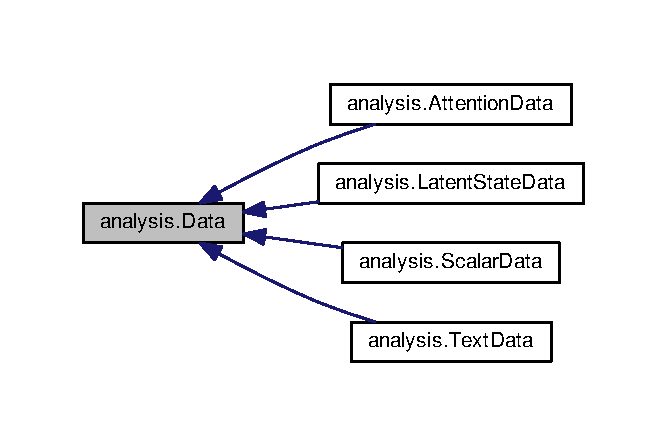
\includegraphics[width=320pt]{classanalysis_1_1Data__inherit__graph}
\end{center}
\end{figure}
\subsection*{Public Member Functions}
\begin{DoxyCompactItemize}
\item 
def {\bfseries \+\_\+\+\_\+init\+\_\+\+\_\+} (self)\hypertarget{classanalysis_1_1Data_a421f903716bc94060deced05ef0be1c4}{}\label{classanalysis_1_1Data_a421f903716bc94060deced05ef0be1c4}

\item 
def {\bfseries add} (self, identifier, value)\hypertarget{classanalysis_1_1Data_a270c5134554c0fcb878c19aa13698489}{}\label{classanalysis_1_1Data_a270c5134554c0fcb878c19aa13698489}

\item 
def {\bfseries get\+\_\+required\+\_\+keys} (self)\hypertarget{classanalysis_1_1Data_ab0735d062f6ad56c2b136ab31068680b}{}\label{classanalysis_1_1Data_ab0735d062f6ad56c2b136ab31068680b}

\item 
def {\bfseries data} (self)\hypertarget{classanalysis_1_1Data_a4d47ba14ef2cef870bdee36aaa0c6f5b}{}\label{classanalysis_1_1Data_a4d47ba14ef2cef870bdee36aaa0c6f5b}

\item 
def {\bfseries identifiers} (self)\hypertarget{classanalysis_1_1Data_ae25a08a00858c9f8f998f1b53320e6ef}{}\label{classanalysis_1_1Data_ae25a08a00858c9f8f998f1b53320e6ef}

\end{DoxyCompactItemize}


\subsection{Detailed Description}
\begin{DoxyVerb}\end{DoxyVerb}
 

The documentation for this class was generated from the following file\+:\begin{DoxyCompactItemize}
\item 
src/utils/analysis.\+py\end{DoxyCompactItemize}

\hypertarget{classanalysis_1_1DataLog}{}\section{analysis.\+Data\+Log Class Reference}
\label{classanalysis_1_1DataLog}\index{analysis.\+Data\+Log@{analysis.\+Data\+Log}}
\subsection*{Public Member Functions}
\begin{DoxyCompactItemize}
\item 
def {\bfseries \+\_\+\+\_\+init\+\_\+\+\_\+} (self, data\+\_\+interface)\hypertarget{classanalysis_1_1DataLog_ab0bb3f72c3261c4a0e1d96242526cbae}{}\label{classanalysis_1_1DataLog_ab0bb3f72c3261c4a0e1d96242526cbae}

\item 
def {\bfseries add} (self, identifier, key, value)\hypertarget{classanalysis_1_1DataLog_a3f99cf1502204b3c1c7a1a41c60ccec4}{}\label{classanalysis_1_1DataLog_a3f99cf1502204b3c1c7a1a41c60ccec4}

\item 
def {\bfseries get\+\_\+required\+\_\+keys} (self, key)\hypertarget{classanalysis_1_1DataLog_af5e78092a36a9d7065afa77ddc0a34b7}{}\label{classanalysis_1_1DataLog_af5e78092a36a9d7065afa77ddc0a34b7}

\item 
def {\bfseries data} (self)\hypertarget{classanalysis_1_1DataLog_a459c8669a4867d4a2dcab963890f42bf}{}\label{classanalysis_1_1DataLog_a459c8669a4867d4a2dcab963890f42bf}

\item 
def {\bfseries identifiers} (self)\hypertarget{classanalysis_1_1DataLog_aed72cd702096ef3c8b6d202233e418c2}{}\label{classanalysis_1_1DataLog_aed72cd702096ef3c8b6d202233e418c2}

\end{DoxyCompactItemize}
\subsection*{Static Public Attributes}
\begin{DoxyCompactItemize}
\item 
{\bfseries str}\hypertarget{classanalysis_1_1DataLog_a92c66f41513976e488b85bb347bb423b}{}\label{classanalysis_1_1DataLog_a92c66f41513976e488b85bb347bb423b}

\end{DoxyCompactItemize}


\subsection{Detailed Description}
\begin{DoxyVerb}\end{DoxyVerb}
 

The documentation for this class was generated from the following file\+:\begin{DoxyCompactItemize}
\item 
src/utils/analysis.\+py\end{DoxyCompactItemize}

\hypertarget{classanalysis_1_1DataLogContainer}{}\section{analysis.\+Data\+Log\+Container Class Reference}
\label{classanalysis_1_1DataLogContainer}\index{analysis.\+Data\+Log\+Container@{analysis.\+Data\+Log\+Container}}
\subsection*{Public Member Functions}
\begin{DoxyCompactItemize}
\item 
def {\bfseries \+\_\+\+\_\+init\+\_\+\+\_\+} (self)\hypertarget{classanalysis_1_1DataLogContainer_a7129c7e32aab8ec87ea3cb166f4f8131}{}\label{classanalysis_1_1DataLogContainer_a7129c7e32aab8ec87ea3cb166f4f8131}

\item 
def {\bfseries add} (self, data\+\_\+logs)\hypertarget{classanalysis_1_1DataLogContainer_afdd353084bd8e8f18d055daf501c7a72}{}\label{classanalysis_1_1DataLogContainer_afdd353084bd8e8f18d055daf501c7a72}

\item 
def {\bfseries display} (self, metric, tokens, identifiers, plot\+\_\+size, epoch\+\_\+range=(None,), kwargs)\hypertarget{classanalysis_1_1DataLogContainer_a928e1b757e08cf446d020e2d4e8d5d2f}{}\label{classanalysis_1_1DataLogContainer_a928e1b757e08cf446d020e2d4e8d5d2f}

\item 
def {\bfseries metrics} (self)\hypertarget{classanalysis_1_1DataLogContainer_a128523601583ae3990beba92b9451c76}{}\label{classanalysis_1_1DataLogContainer_a128523601583ae3990beba92b9451c76}

\end{DoxyCompactItemize}


\subsection{Detailed Description}
\begin{DoxyVerb}\end{DoxyVerb}
 

The documentation for this class was generated from the following file\+:\begin{DoxyCompactItemize}
\item 
src/utils/analysis.\+py\end{DoxyCompactItemize}

\hypertarget{classreader_1_1DataQueue}{}\section{reader.\+Data\+Queue Class Reference}
\label{classreader_1_1DataQueue}\index{reader.\+Data\+Queue@{reader.\+Data\+Queue}}
\subsection*{Public Member Functions}
\begin{DoxyCompactItemize}
\item 
def {\bfseries \+\_\+\+\_\+init\+\_\+\+\_\+}\hypertarget{classreader_1_1DataQueue_ab9a2c9d3fef5991b47b2c5e4ada7a4e8}{}\label{classreader_1_1DataQueue_ab9a2c9d3fef5991b47b2c5e4ada7a4e8}

\item 
def \hyperlink{classreader_1_1DataQueue_af6e14dd0a81e37dcff0a69044f3c9a01}{measure\+\_\+length} (self)
\item 
def \hyperlink{classreader_1_1DataQueue_a4b4fd15ec3b96973451d120c8f8afcbf}{generator} (self)
\end{DoxyCompactItemize}
\subsection*{Static Public Attributes}
\begin{DoxyCompactItemize}
\item 
int {\bfseries M\+A\+X\+\_\+\+S\+E\+G\+M\+E\+NT} = 500000\hypertarget{classreader_1_1DataQueue_a786dc7054b64a7a3aac0f9a23cdd6bf0}{}\label{classreader_1_1DataQueue_a786dc7054b64a7a3aac0f9a23cdd6bf0}

\end{DoxyCompactItemize}


\subsection{Detailed Description}
\begin{DoxyVerb}A queue object for the data feed. This can be later configured to load the data to
memory asynchronously.
\end{DoxyVerb}
 

\subsection{Member Function Documentation}
\index{reader\+::\+Data\+Queue@{reader\+::\+Data\+Queue}!generator@{generator}}
\index{generator@{generator}!reader\+::\+Data\+Queue@{reader\+::\+Data\+Queue}}
\subsubsection[{\texorpdfstring{generator(self)}{generator(self)}}]{\setlength{\rightskip}{0pt plus 5cm}def reader.\+Data\+Queue.\+generator (
\begin{DoxyParamCaption}
\item[{}]{self, }
\item[{}]{list}
\end{DoxyParamCaption}
)}\hypertarget{classreader_1_1DataQueue_a4b4fd15ec3b96973451d120c8f8afcbf}{}\label{classreader_1_1DataQueue_a4b4fd15ec3b96973451d120c8f8afcbf}
\begin{DoxyVerb}Data is retrieved directly from a file, and loaded into data chunks of size MAX_CHUNK_SIZE.
\end{DoxyVerb}
 \index{reader\+::\+Data\+Queue@{reader\+::\+Data\+Queue}!measure\+\_\+length@{measure\+\_\+length}}
\index{measure\+\_\+length@{measure\+\_\+length}!reader\+::\+Data\+Queue@{reader\+::\+Data\+Queue}}
\subsubsection[{\texorpdfstring{measure\+\_\+length(self)}{measure_length(self)}}]{\setlength{\rightskip}{0pt plus 5cm}def reader.\+Data\+Queue.\+measure\+\_\+length (
\begin{DoxyParamCaption}
\item[{}]{self, }
\item[{}]{int}
\end{DoxyParamCaption}
)}\hypertarget{classreader_1_1DataQueue_af6e14dd0a81e37dcff0a69044f3c9a01}{}\label{classreader_1_1DataQueue_af6e14dd0a81e37dcff0a69044f3c9a01}
\begin{DoxyVerb}Measures the length of the corpora file.
\end{DoxyVerb}
 

The documentation for this class was generated from the following file\+:\begin{DoxyCompactItemize}
\item 
src/utils/reader.\+py\end{DoxyCompactItemize}

\hypertarget{classbase_1_1Decoder}{}\section{base.\+Decoder Class Reference}
\label{classbase_1_1Decoder}\index{base.\+Decoder@{base.\+Decoder}}


Inheritance diagram for base.\+Decoder\+:
\nopagebreak
\begin{figure}[H]
\begin{center}
\leavevmode
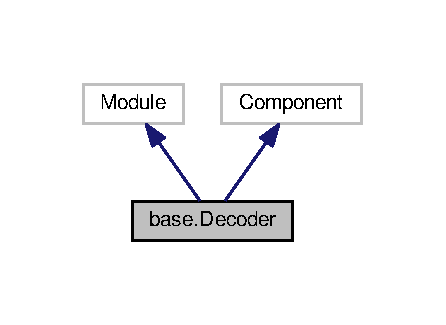
\includegraphics[width=214pt]{classbase_1_1Decoder__inherit__graph}
\end{center}
\end{figure}


Collaboration diagram for base.\+Decoder\+:
\nopagebreak
\begin{figure}[H]
\begin{center}
\leavevmode
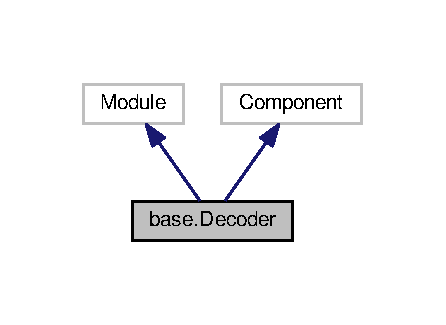
\includegraphics[width=214pt]{classbase_1_1Decoder__coll__graph}
\end{center}
\end{figure}
\subsection*{Public Member Functions}
\begin{DoxyCompactItemize}
\item 
def {\bfseries \+\_\+\+\_\+init\+\_\+\+\_\+} (self, args, kwargs)\hypertarget{classbase_1_1Decoder_a88d9b648b9da9127c78b05ed0a6df34f}{}\label{classbase_1_1Decoder_a88d9b648b9da9127c78b05ed0a6df34f}

\item 
def {\bfseries forward} (self, args, kwargs)\hypertarget{classbase_1_1Decoder_ac6711e9af0b7ab314a528c413f2ab620}{}\label{classbase_1_1Decoder_ac6711e9af0b7ab314a528c413f2ab620}

\item 
def {\bfseries optimizers} (self)\hypertarget{classbase_1_1Decoder_aa81fcc7acc9aeaa2f46adfa708bd9b04}{}\label{classbase_1_1Decoder_aa81fcc7acc9aeaa2f46adfa708bd9b04}

\item 
def {\bfseries state} (self)\hypertarget{classbase_1_1Decoder_a9192c673b5fa6baee20e824e17510f96}{}\label{classbase_1_1Decoder_a9192c673b5fa6baee20e824e17510f96}

\item 
def {\bfseries state} (self, value)\hypertarget{classbase_1_1Decoder_adf38a0b19e1a15de7073ccc9beeda86d}{}\label{classbase_1_1Decoder_adf38a0b19e1a15de7073ccc9beeda86d}

\item 
def {\bfseries output\+\_\+size} (self)\hypertarget{classbase_1_1Decoder_a1f31b5d3c97caf158899ec4f11d6abf4}{}\label{classbase_1_1Decoder_a1f31b5d3c97caf158899ec4f11d6abf4}

\end{DoxyCompactItemize}


\subsection{Detailed Description}
\begin{DoxyVerb}Abstract base class for the decoder modules of the application. A decoder must
inherit from this class, otherwise it won't be discoverable by the hierarchy
builder utility.
\end{DoxyVerb}
 

The documentation for this class was generated from the following file\+:\begin{DoxyCompactItemize}
\item 
src/components/base.\+py\end{DoxyCompactItemize}

\hypertarget{classmodules_1_1Discriminator}{}\section{modules.\+Discriminator Class Reference}
\label{classmodules_1_1Discriminator}\index{modules.\+Discriminator@{modules.\+Discriminator}}
\subsection*{Public Member Functions}
\begin{DoxyCompactItemize}
\item 
def {\bfseries \+\_\+\+\_\+init\+\_\+\+\_\+}\hypertarget{classmodules_1_1Discriminator_ae79430af96ad263034049ba01e1e2c8f}{}\label{classmodules_1_1Discriminator_ae79430af96ad263034049ba01e1e2c8f}

\item 
def \hyperlink{classmodules_1_1Discriminator_ad8ff9ec051ea2b440af48108d2e5bfdb}{\+\_\+\+\_\+call\+\_\+\+\_\+} (self, args, inputs, targets, kwargs)
\end{DoxyCompactItemize}


\subsection{Detailed Description}
\begin{DoxyVerb}\end{DoxyVerb}
 

\subsection{Member Function Documentation}
\index{modules\+::\+Discriminator@{modules\+::\+Discriminator}!\+\_\+\+\_\+call\+\_\+\+\_\+@{\+\_\+\+\_\+call\+\_\+\+\_\+}}
\index{\+\_\+\+\_\+call\+\_\+\+\_\+@{\+\_\+\+\_\+call\+\_\+\+\_\+}!modules\+::\+Discriminator@{modules\+::\+Discriminator}}
\subsubsection[{\texorpdfstring{\+\_\+\+\_\+call\+\_\+\+\_\+(self, args, inputs, targets, kwargs)}{__call__(self, args, inputs, targets, kwargs)}}]{\setlength{\rightskip}{0pt plus 5cm}def modules.\+Discriminator.\+\_\+\+\_\+call\+\_\+\+\_\+ (
\begin{DoxyParamCaption}
\item[{}]{self, }
\item[{}]{args, }
\item[{}]{inputs, }
\item[{}]{targets, }
\item[{}]{kwargs}
\end{DoxyParamCaption}
)}\hypertarget{classmodules_1_1Discriminator_ad8ff9ec051ea2b440af48108d2e5bfdb}{}\label{classmodules_1_1Discriminator_ad8ff9ec051ea2b440af48108d2e5bfdb}
\begin{DoxyVerb}This function implements the discrimination mechanism, where the inputs and the targets - which
are required for the evaluation and training of the discriminator - are created. The inputs are
fed into the discriminator and evaluated based on the cross entropy loss, that is defined in the
init function. The targets are either one-hot coded vectors, or their inverse. This depends on
whether the loss is calculated for the discriminator or model loss.

:param inputs:
    A list, containing the batches from the input pipelines.

:param targets:
    An int value, that represents the index of the encoder's input language.

:param lengths:

:return loss:
    A scalar loss value, indicating the average loss of the discriminator for either the
    inverse or normal target vector.
\end{DoxyVerb}
 

The documentation for this class was generated from the following file\+:\begin{DoxyCompactItemize}
\item 
src/modules/modules.\+py\end{DoxyCompactItemize}

\hypertarget{classexperiments_1_1DividedCurriculumTranslation}{}\section{experiments.\+Divided\+Curriculum\+Translation Class Reference}
\label{classexperiments_1_1DividedCurriculumTranslation}\index{experiments.\+Divided\+Curriculum\+Translation@{experiments.\+Divided\+Curriculum\+Translation}}


Inheritance diagram for experiments.\+Divided\+Curriculum\+Translation\+:
\nopagebreak
\begin{figure}[H]
\begin{center}
\leavevmode
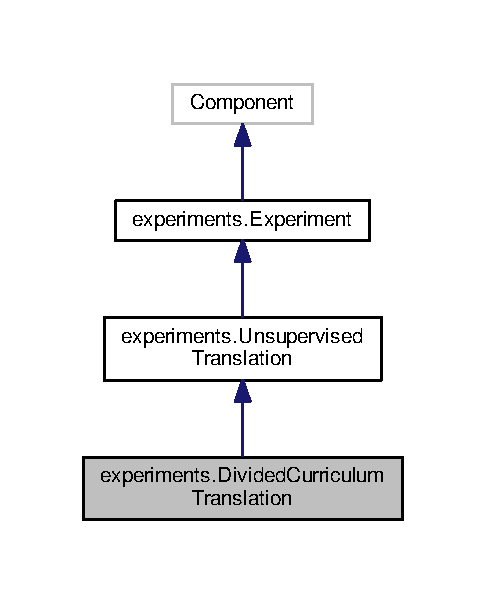
\includegraphics[width=233pt]{classexperiments_1_1DividedCurriculumTranslation__inherit__graph}
\end{center}
\end{figure}


Collaboration diagram for experiments.\+Divided\+Curriculum\+Translation\+:
\nopagebreak
\begin{figure}[H]
\begin{center}
\leavevmode
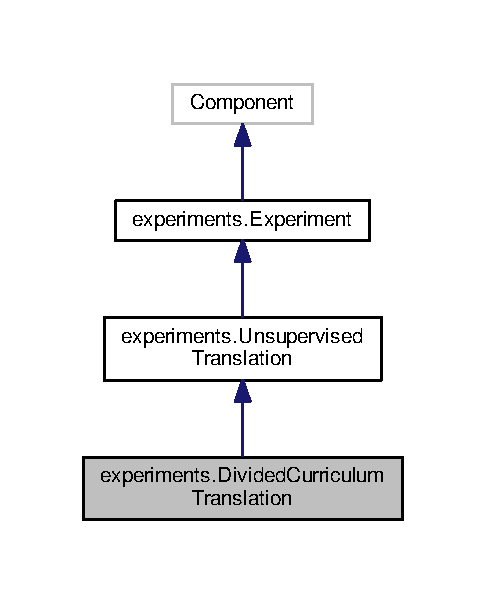
\includegraphics[width=233pt]{classexperiments_1_1DividedCurriculumTranslation__coll__graph}
\end{center}
\end{figure}
\subsection*{Additional Inherited Members}


The documentation for this class was generated from the following file\+:\begin{DoxyCompactItemize}
\item 
src/experiments/experiments.\+py\end{DoxyCompactItemize}

\hypertarget{classrnn_1_1DotAttentionRNNDecoder}{}\section{rnn.\+Dot\+Attention\+R\+N\+N\+Decoder Class Reference}
\label{classrnn_1_1DotAttentionRNNDecoder}\index{rnn.\+Dot\+Attention\+R\+N\+N\+Decoder@{rnn.\+Dot\+Attention\+R\+N\+N\+Decoder}}


Inheritance diagram for rnn.\+Dot\+Attention\+R\+N\+N\+Decoder\+:
\nopagebreak
\begin{figure}[H]
\begin{center}
\leavevmode
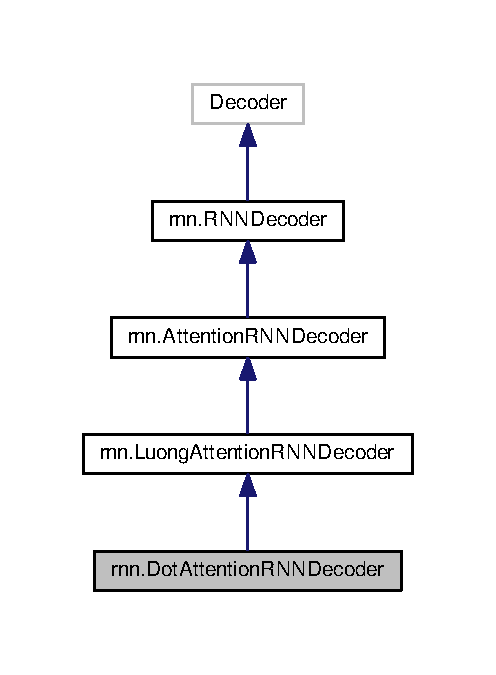
\includegraphics[width=238pt]{classrnn_1_1DotAttentionRNNDecoder__inherit__graph}
\end{center}
\end{figure}


Collaboration diagram for rnn.\+Dot\+Attention\+R\+N\+N\+Decoder\+:
\nopagebreak
\begin{figure}[H]
\begin{center}
\leavevmode
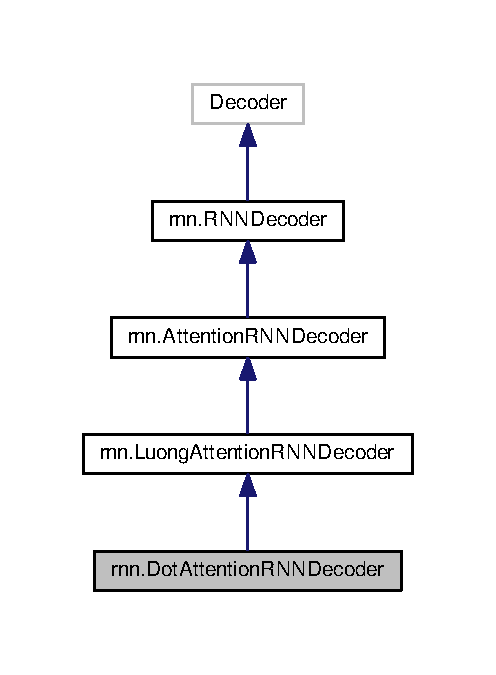
\includegraphics[width=238pt]{classrnn_1_1DotAttentionRNNDecoder__coll__graph}
\end{center}
\end{figure}
\subsection*{Public Member Functions}
\begin{DoxyCompactItemize}
\item 
def {\bfseries \+\_\+\+\_\+init\+\_\+\+\_\+}\hypertarget{classrnn_1_1DotAttentionRNNDecoder_a6eea546565f762ee83ff51c28e1645d4}{}\label{classrnn_1_1DotAttentionRNNDecoder_a6eea546565f762ee83ff51c28e1645d4}

\item 
def \hyperlink{classrnn_1_1DotAttentionRNNDecoder_a0bbac7d4dc05b35c0873c6d0074d6499}{init\+\_\+parameters} (self)
\end{DoxyCompactItemize}
\subsection*{Static Public Attributes}
\begin{DoxyCompactItemize}
\item 
{\bfseries interface} = R\+N\+N\+Decoder.\+interface\hypertarget{classrnn_1_1DotAttentionRNNDecoder_a8f77e3e523eaf8d375280e22818a72e0}{}\label{classrnn_1_1DotAttentionRNNDecoder_a8f77e3e523eaf8d375280e22818a72e0}

\item 
bool {\bfseries abstract} = False\hypertarget{classrnn_1_1DotAttentionRNNDecoder_a6b36fac841800f586bbfa7670003d669}{}\label{classrnn_1_1DotAttentionRNNDecoder_a6b36fac841800f586bbfa7670003d669}

\end{DoxyCompactItemize}
\subsection*{Additional Inherited Members}


\subsection{Detailed Description}
\begin{DoxyVerb}Global attention mechanism for the recurrent decoder module. The algorithm is a specific case
of Luong style attention, where the scoring is based off of only the dot product of the
encoder and decoder states.
\end{DoxyVerb}
 

\subsection{Member Function Documentation}
\index{rnn\+::\+Dot\+Attention\+R\+N\+N\+Decoder@{rnn\+::\+Dot\+Attention\+R\+N\+N\+Decoder}!init\+\_\+parameters@{init\+\_\+parameters}}
\index{init\+\_\+parameters@{init\+\_\+parameters}!rnn\+::\+Dot\+Attention\+R\+N\+N\+Decoder@{rnn\+::\+Dot\+Attention\+R\+N\+N\+Decoder}}
\subsubsection[{\texorpdfstring{init\+\_\+parameters(self)}{init_parameters(self)}}]{\setlength{\rightskip}{0pt plus 5cm}def rnn.\+Dot\+Attention\+R\+N\+N\+Decoder.\+init\+\_\+parameters (
\begin{DoxyParamCaption}
\item[{}]{self, }
\item[{}]{Decoder}
\end{DoxyParamCaption}
)}\hypertarget{classrnn_1_1DotAttentionRNNDecoder_a0bbac7d4dc05b35c0873c6d0074d6499}{}\label{classrnn_1_1DotAttentionRNNDecoder_a0bbac7d4dc05b35c0873c6d0074d6499}
\begin{DoxyVerb}Initializes the parameters for the decoder.
\end{DoxyVerb}
 

The documentation for this class was generated from the following file\+:\begin{DoxyCompactItemize}
\item 
src/components/decoders/rnn.\+py\end{DoxyCompactItemize}

\hypertarget{classutils_1_1Embedding}{}\section{utils.\+Embedding Class Reference}
\label{classutils_1_1Embedding}\index{utils.\+Embedding@{utils.\+Embedding}}


Inheritance diagram for utils.\+Embedding\+:
\nopagebreak
\begin{figure}[H]
\begin{center}
\leavevmode
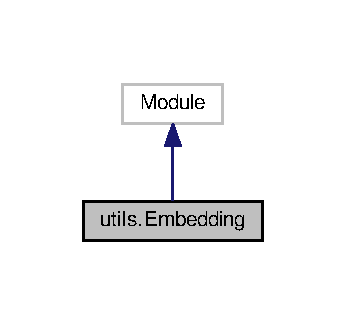
\includegraphics[width=166pt]{classutils_1_1Embedding__inherit__graph}
\end{center}
\end{figure}


Collaboration diagram for utils.\+Embedding\+:
\nopagebreak
\begin{figure}[H]
\begin{center}
\leavevmode
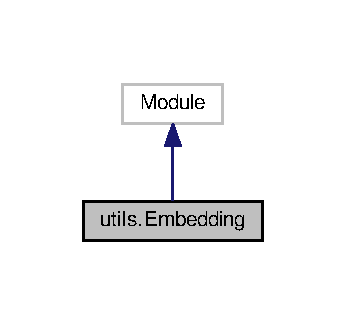
\includegraphics[width=166pt]{classutils_1_1Embedding__coll__graph}
\end{center}
\end{figure}
\subsection*{Public Member Functions}
\begin{DoxyCompactItemize}
\item 
def {\bfseries \+\_\+\+\_\+init\+\_\+\+\_\+}\hypertarget{classutils_1_1Embedding_a5022555fe31ce2e41e72c466362a3c01}{}\label{classutils_1_1Embedding_a5022555fe31ce2e41e72c466362a3c01}

\item 
def \hyperlink{classutils_1_1Embedding_ac21374958141a3f27191d873b107edf5}{forward} (self, inputs)
\item 
def \hyperlink{classutils_1_1Embedding_a7726f478edc24c481f103d71e92e1bf2}{freeze} (self)
\item 
def \hyperlink{classutils_1_1Embedding_afd03315bbaada52bbf08dd34a3353693}{unfreeze} (self)
\item 
def \hyperlink{classutils_1_1Embedding_a6e89544aab0d191a209558c5d93bd79f}{optimizer} (self)
\item 
def \hyperlink{classutils_1_1Embedding_a1a6284d9ed1ebba9515448b194d1c47f}{state} (self)
\item 
def \hyperlink{classutils_1_1Embedding_a68b81dd7e2446c7b7a7d17d9eb2c7f80}{state} (self, states)
\end{DoxyCompactItemize}


\subsection{Detailed Description}
\begin{DoxyVerb}Wrapper class for the embedding layers of the models. The optional training of the embeddings
is done by a built-in optimizer.
\end{DoxyVerb}
 

\subsection{Member Function Documentation}
\index{utils\+::\+Embedding@{utils\+::\+Embedding}!forward@{forward}}
\index{forward@{forward}!utils\+::\+Embedding@{utils\+::\+Embedding}}
\subsubsection[{\texorpdfstring{forward(self, inputs)}{forward(self, inputs)}}]{\setlength{\rightskip}{0pt plus 5cm}def utils.\+Embedding.\+forward (
\begin{DoxyParamCaption}
\item[{}]{self, }
\item[{}]{inputs}
\end{DoxyParamCaption}
)}\hypertarget{classutils_1_1Embedding_ac21374958141a3f27191d873b107edf5}{}\label{classutils_1_1Embedding_ac21374958141a3f27191d873b107edf5}
\begin{DoxyVerb}Propagates the inputs through the embedding layer.

:param inputs:
    Variable, word id-s, that will be translated to word vector representations.

:return outputs:
    Variable, word vectors of the given input.
\end{DoxyVerb}
 \index{utils\+::\+Embedding@{utils\+::\+Embedding}!freeze@{freeze}}
\index{freeze@{freeze}!utils\+::\+Embedding@{utils\+::\+Embedding}}
\subsubsection[{\texorpdfstring{freeze(self)}{freeze(self)}}]{\setlength{\rightskip}{0pt plus 5cm}def utils.\+Embedding.\+freeze (
\begin{DoxyParamCaption}
\item[{}]{self}
\end{DoxyParamCaption}
)}\hypertarget{classutils_1_1Embedding_a7726f478edc24c481f103d71e92e1bf2}{}\label{classutils_1_1Embedding_a7726f478edc24c481f103d71e92e1bf2}
\begin{DoxyVerb}Freezes the parameters of the embedding layer. While frozen, the parameters can't be
modified by the optimizer.
\end{DoxyVerb}
 \index{utils\+::\+Embedding@{utils\+::\+Embedding}!optimizer@{optimizer}}
\index{optimizer@{optimizer}!utils\+::\+Embedding@{utils\+::\+Embedding}}
\subsubsection[{\texorpdfstring{optimizer(self)}{optimizer(self)}}]{\setlength{\rightskip}{0pt plus 5cm}def utils.\+Embedding.\+optimizer (
\begin{DoxyParamCaption}
\item[{}]{self}
\end{DoxyParamCaption}
)}\hypertarget{classutils_1_1Embedding_a6e89544aab0d191a209558c5d93bd79f}{}\label{classutils_1_1Embedding_a6e89544aab0d191a209558c5d93bd79f}
\begin{DoxyVerb}Property for the optimizer of the embedding.
\end{DoxyVerb}
 \index{utils\+::\+Embedding@{utils\+::\+Embedding}!state@{state}}
\index{state@{state}!utils\+::\+Embedding@{utils\+::\+Embedding}}
\subsubsection[{\texorpdfstring{state(self)}{state(self)}}]{\setlength{\rightskip}{0pt plus 5cm}def utils.\+Embedding.\+state (
\begin{DoxyParamCaption}
\item[{}]{self}
\end{DoxyParamCaption}
)}\hypertarget{classutils_1_1Embedding_a1a6284d9ed1ebba9515448b194d1c47f}{}\label{classutils_1_1Embedding_a1a6284d9ed1ebba9515448b194d1c47f}
\begin{DoxyVerb}Property for the state of the embedding.
\end{DoxyVerb}
 \index{utils\+::\+Embedding@{utils\+::\+Embedding}!state@{state}}
\index{state@{state}!utils\+::\+Embedding@{utils\+::\+Embedding}}
\subsubsection[{\texorpdfstring{state(self, states)}{state(self, states)}}]{\setlength{\rightskip}{0pt plus 5cm}def utils.\+Embedding.\+state (
\begin{DoxyParamCaption}
\item[{}]{self, }
\item[{}]{states}
\end{DoxyParamCaption}
)}\hypertarget{classutils_1_1Embedding_a68b81dd7e2446c7b7a7d17d9eb2c7f80}{}\label{classutils_1_1Embedding_a68b81dd7e2446c7b7a7d17d9eb2c7f80}
\begin{DoxyVerb}Setter method for the state of the embedding.
\end{DoxyVerb}
 \index{utils\+::\+Embedding@{utils\+::\+Embedding}!unfreeze@{unfreeze}}
\index{unfreeze@{unfreeze}!utils\+::\+Embedding@{utils\+::\+Embedding}}
\subsubsection[{\texorpdfstring{unfreeze(self)}{unfreeze(self)}}]{\setlength{\rightskip}{0pt plus 5cm}def utils.\+Embedding.\+unfreeze (
\begin{DoxyParamCaption}
\item[{}]{self}
\end{DoxyParamCaption}
)}\hypertarget{classutils_1_1Embedding_afd03315bbaada52bbf08dd34a3353693}{}\label{classutils_1_1Embedding_afd03315bbaada52bbf08dd34a3353693}
\begin{DoxyVerb}       Unfreezes the parameters of the optimizers. By calling this method, the optimizer will
       be able to modify the weights of the embedding layer.\end{DoxyVerb}
 

The documentation for this class was generated from the following file\+:\begin{DoxyCompactItemize}
\item 
src/components/utils/utils.\+py\end{DoxyCompactItemize}

\hypertarget{classbase_1_1Encoder}{}\section{base.\+Encoder Class Reference}
\label{classbase_1_1Encoder}\index{base.\+Encoder@{base.\+Encoder}}


Inheritance diagram for base.\+Encoder\+:
\nopagebreak
\begin{figure}[H]
\begin{center}
\leavevmode
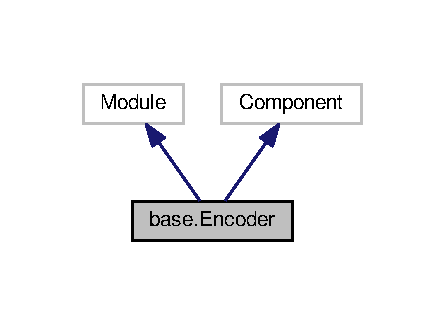
\includegraphics[width=214pt]{classbase_1_1Encoder__inherit__graph}
\end{center}
\end{figure}


Collaboration diagram for base.\+Encoder\+:
\nopagebreak
\begin{figure}[H]
\begin{center}
\leavevmode
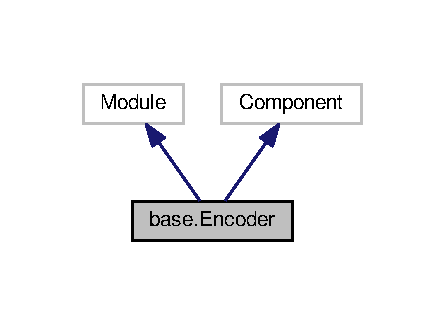
\includegraphics[width=214pt]{classbase_1_1Encoder__coll__graph}
\end{center}
\end{figure}
\subsection*{Public Member Functions}
\begin{DoxyCompactItemize}
\item 
def {\bfseries \+\_\+\+\_\+init\+\_\+\+\_\+} (self, args, kwargs)\hypertarget{classbase_1_1Encoder_af514ec6b1374cc03b81f8487a47133b9}{}\label{classbase_1_1Encoder_af514ec6b1374cc03b81f8487a47133b9}

\item 
def {\bfseries forward} (self, args, kwargs)\hypertarget{classbase_1_1Encoder_a8dab70aa94cd40cb0e593b83e99a5703}{}\label{classbase_1_1Encoder_a8dab70aa94cd40cb0e593b83e99a5703}

\item 
def {\bfseries optimizers} (self)\hypertarget{classbase_1_1Encoder_af3bbb9f6332fb18878b67ccb61f9cb76}{}\label{classbase_1_1Encoder_af3bbb9f6332fb18878b67ccb61f9cb76}

\item 
def {\bfseries state} (self)\hypertarget{classbase_1_1Encoder_a3daeae83d0344416ce9d3e96cac6ae24}{}\label{classbase_1_1Encoder_a3daeae83d0344416ce9d3e96cac6ae24}

\item 
def {\bfseries state} (self, value)\hypertarget{classbase_1_1Encoder_a1b581db8dc18b9ceb95a57372ca9447c}{}\label{classbase_1_1Encoder_a1b581db8dc18b9ceb95a57372ca9447c}

\end{DoxyCompactItemize}


\subsection{Detailed Description}
\begin{DoxyVerb}Abstract base class for the encoder modules of the application. An encoder must
inherit from this class, otherwise it won't be discoverable by the hierarchy
builder utility.
\end{DoxyVerb}
 

The documentation for this class was generated from the following file\+:\begin{DoxyCompactItemize}
\item 
src/components/base.\+py\end{DoxyCompactItemize}

\hypertarget{classsession_1_1EvaluationContext}{}\section{session.\+Evaluation\+Context Class Reference}
\label{classsession_1_1EvaluationContext}\index{session.\+Evaluation\+Context@{session.\+Evaluation\+Context}}
\subsection*{Public Member Functions}
\begin{DoxyCompactItemize}
\item 
def {\bfseries \+\_\+\+\_\+init\+\_\+\+\_\+} (self, session)\hypertarget{classsession_1_1EvaluationContext_af632e4b9548697bb4746dd311acf1ba8}{}\label{classsession_1_1EvaluationContext_af632e4b9548697bb4746dd311acf1ba8}

\item 
def {\bfseries \+\_\+\+\_\+enter\+\_\+\+\_\+} (self)\hypertarget{classsession_1_1EvaluationContext_a86f2b7ec1b6da4daf1de2c7a6ea7cf74}{}\label{classsession_1_1EvaluationContext_a86f2b7ec1b6da4daf1de2c7a6ea7cf74}

\item 
def {\bfseries \+\_\+\+\_\+exit\+\_\+\+\_\+} (self, exc\+\_\+type, exc\+\_\+val, exc\+\_\+tb)\hypertarget{classsession_1_1EvaluationContext_a0595f94dad0457edaff2b91625ee097d}{}\label{classsession_1_1EvaluationContext_a0595f94dad0457edaff2b91625ee097d}

\item 
def {\bfseries evaluate} (self)\hypertarget{classsession_1_1EvaluationContext_a73262545d159ef7d94d72d205274630e}{}\label{classsession_1_1EvaluationContext_a73262545d159ef7d94d72d205274630e}

\item 
def {\bfseries save} (self)\hypertarget{classsession_1_1EvaluationContext_a5f63c9bf32f8581ac474543a864c1742}{}\label{classsession_1_1EvaluationContext_a5f63c9bf32f8581ac474543a864c1742}

\end{DoxyCompactItemize}
\subsection*{Static Public Attributes}
\begin{DoxyCompactItemize}
\item 
string {\bfseries E\+V\+A\+L\+\_\+\+F\+I\+LE} = \textquotesingle{}eval.\+pt\textquotesingle{}\hypertarget{classsession_1_1EvaluationContext_a0a54ef1a53ca4a5fc7074b3eb16910be}{}\label{classsession_1_1EvaluationContext_a0a54ef1a53ca4a5fc7074b3eb16910be}

\end{DoxyCompactItemize}


The documentation for this class was generated from the following file\+:\begin{DoxyCompactItemize}
\item 
src/utils/session.\+py\end{DoxyCompactItemize}

\hypertarget{classexperiments_1_1Experiment}{}\section{experiments.\+Experiment Class Reference}
\label{classexperiments_1_1Experiment}\index{experiments.\+Experiment@{experiments.\+Experiment}}


Inheritance diagram for experiments.\+Experiment\+:
\nopagebreak
\begin{figure}[H]
\begin{center}
\leavevmode
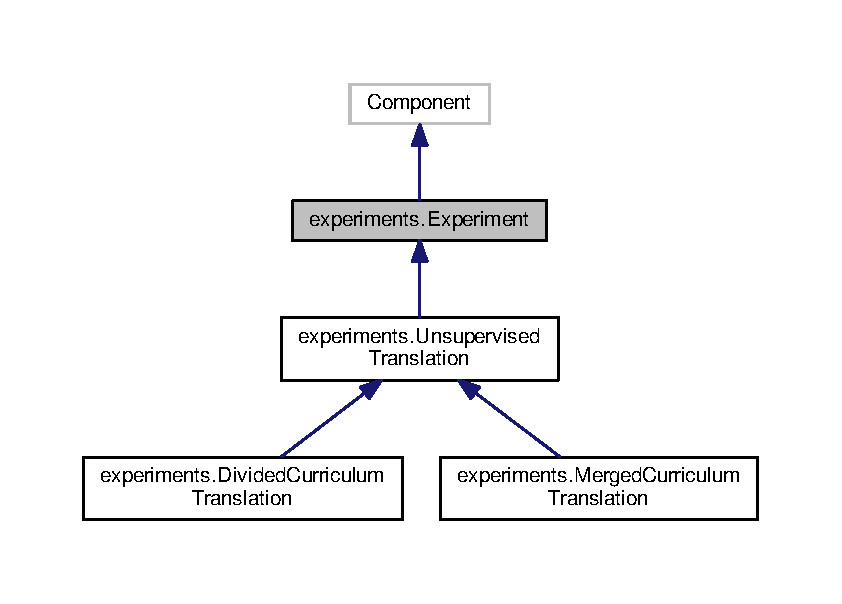
\includegraphics[width=350pt]{classexperiments_1_1Experiment__inherit__graph}
\end{center}
\end{figure}


Collaboration diagram for experiments.\+Experiment\+:
\nopagebreak
\begin{figure}[H]
\begin{center}
\leavevmode
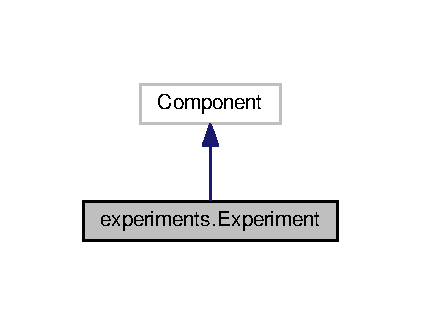
\includegraphics[width=202pt]{classexperiments_1_1Experiment__coll__graph}
\end{center}
\end{figure}
\subsection*{Public Member Functions}
\begin{DoxyCompactItemize}
\item 
def {\bfseries train} (self, epoch)\hypertarget{classexperiments_1_1Experiment_acc2a8ad8030038ea2d891099edd286f5}{}\label{classexperiments_1_1Experiment_acc2a8ad8030038ea2d891099edd286f5}

\item 
def {\bfseries validate} (self)\hypertarget{classexperiments_1_1Experiment_ab652dc0daa8b93841258060f6c8f9376}{}\label{classexperiments_1_1Experiment_ab652dc0daa8b93841258060f6c8f9376}

\item 
def {\bfseries test} (self)\hypertarget{classexperiments_1_1Experiment_aa21f617378a3b6648db5bf9ee407babf}{}\label{classexperiments_1_1Experiment_aa21f617378a3b6648db5bf9ee407babf}

\item 
def {\bfseries evaluate} (self)\hypertarget{classexperiments_1_1Experiment_a2eb3e3401304334fc2ee5a198b5da7b7}{}\label{classexperiments_1_1Experiment_a2eb3e3401304334fc2ee5a198b5da7b7}

\item 
def {\bfseries state} (self)\hypertarget{classexperiments_1_1Experiment_a911083453a831d45a0e9938de2f0e8b7}{}\label{classexperiments_1_1Experiment_a911083453a831d45a0e9938de2f0e8b7}

\item 
def {\bfseries state} (self, value)\hypertarget{classexperiments_1_1Experiment_ac4abf41c48de38c2485a60307bdde0e3}{}\label{classexperiments_1_1Experiment_ac4abf41c48de38c2485a60307bdde0e3}

\end{DoxyCompactItemize}


\subsection{Detailed Description}
\begin{DoxyVerb}Abstract base class for the experiments.
\end{DoxyVerb}
 

The documentation for this class was generated from the following file\+:\begin{DoxyCompactItemize}
\item 
src/experiments/experiments.\+py\end{DoxyCompactItemize}

\hypertarget{classutils_1_1FFClassifier}{}\section{utils.\+F\+F\+Classifier Class Reference}
\label{classutils_1_1FFClassifier}\index{utils.\+F\+F\+Classifier@{utils.\+F\+F\+Classifier}}


Inheritance diagram for utils.\+F\+F\+Classifier\+:
\nopagebreak
\begin{figure}[H]
\begin{center}
\leavevmode
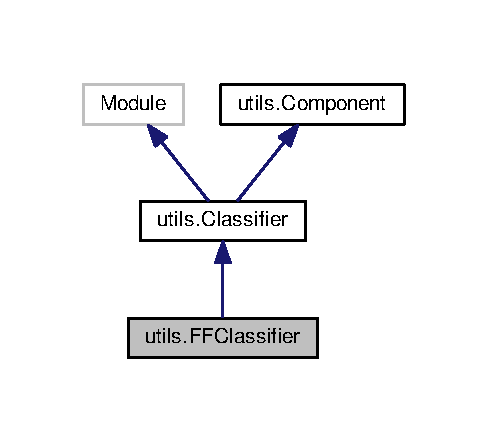
\includegraphics[width=234pt]{classutils_1_1FFClassifier__inherit__graph}
\end{center}
\end{figure}


Collaboration diagram for utils.\+F\+F\+Classifier\+:
\nopagebreak
\begin{figure}[H]
\begin{center}
\leavevmode
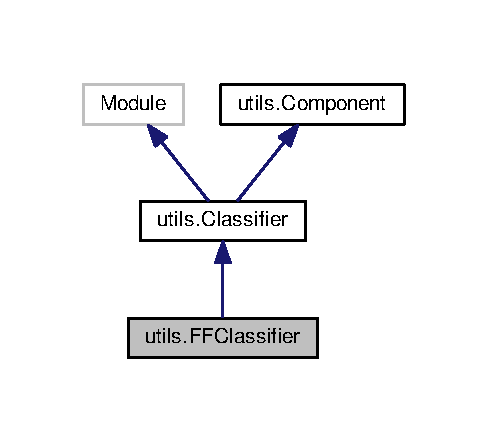
\includegraphics[width=234pt]{classutils_1_1FFClassifier__coll__graph}
\end{center}
\end{figure}
\subsection*{Public Member Functions}
\begin{DoxyCompactItemize}
\item 
def {\bfseries \+\_\+\+\_\+init\+\_\+\+\_\+}\hypertarget{classutils_1_1FFClassifier_ad062320ee3630de6390d22b5d341ce4e}{}\label{classutils_1_1FFClassifier_ad062320ee3630de6390d22b5d341ce4e}

\item 
def \hyperlink{classutils_1_1FFClassifier_a13e7dc081218b4da11d413dcfe492ab7}{forward} (self, args, inputs, kwargs)
\item 
def {\bfseries optimizer} (self)\hypertarget{classutils_1_1FFClassifier_a372b0bea964edaf06d05b897a5d53b53}{}\label{classutils_1_1FFClassifier_a372b0bea964edaf06d05b897a5d53b53}

\end{DoxyCompactItemize}
\subsection*{Static Public Attributes}
\begin{DoxyCompactItemize}
\item 
bool {\bfseries abstract} = False\hypertarget{classutils_1_1FFClassifier_ac92dc5e5ff81ee98204a267e52b09091}{}\label{classutils_1_1FFClassifier_ac92dc5e5ff81ee98204a267e52b09091}

\end{DoxyCompactItemize}


\subsection{Detailed Description}
\begin{DoxyVerb}Feed-forward classifier module for the unsupervised neural translation task.
\end{DoxyVerb}
 

\subsection{Member Function Documentation}
\index{utils\+::\+F\+F\+Classifier@{utils\+::\+F\+F\+Classifier}!forward@{forward}}
\index{forward@{forward}!utils\+::\+F\+F\+Classifier@{utils\+::\+F\+F\+Classifier}}
\subsubsection[{\texorpdfstring{forward(self, args, inputs, kwargs)}{forward(self, args, inputs, kwargs)}}]{\setlength{\rightskip}{0pt plus 5cm}def utils.\+F\+F\+Classifier.\+forward (
\begin{DoxyParamCaption}
\item[{}]{self, }
\item[{}]{args, }
\item[{}]{inputs, }
\item[{}]{kwargs}
\end{DoxyParamCaption}
)}\hypertarget{classutils_1_1FFClassifier_a13e7dc081218b4da11d413dcfe492ab7}{}\label{classutils_1_1FFClassifier_a13e7dc081218b4da11d413dcfe492ab7}
\begin{DoxyVerb}Forward step for the classifier.

:param inputs:
    Variable, (batch_size, input_size), where input_size is equal to the encoder's
    hidden_size.

:return output:
    Variable, (batch_size, 1).
\end{DoxyVerb}
 

The documentation for this class was generated from the following file\+:\begin{DoxyCompactItemize}
\item 
src/components/utils/utils.\+py\end{DoxyCompactItemize}

\hypertarget{classreader_1_1FileInput}{}\section{reader.\+File\+Input Class Reference}
\label{classreader_1_1FileInput}\index{reader.\+File\+Input@{reader.\+File\+Input}}


Inheritance diagram for reader.\+File\+Input\+:
\nopagebreak
\begin{figure}[H]
\begin{center}
\leavevmode
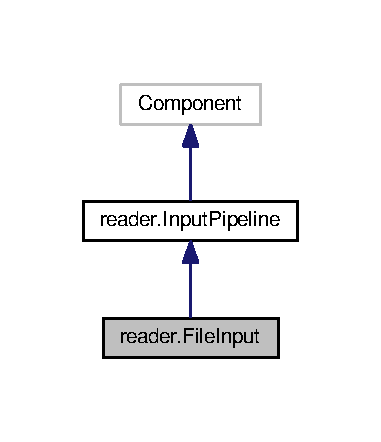
\includegraphics[width=183pt]{classreader_1_1FileInput__inherit__graph}
\end{center}
\end{figure}


Collaboration diagram for reader.\+File\+Input\+:
\nopagebreak
\begin{figure}[H]
\begin{center}
\leavevmode
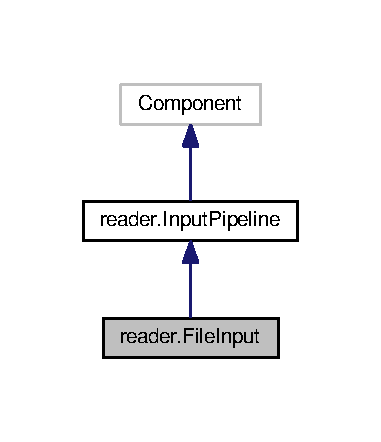
\includegraphics[width=183pt]{classreader_1_1FileInput__coll__graph}
\end{center}
\end{figure}
\subsection*{Public Member Functions}
\begin{DoxyCompactItemize}
\item 
def {\bfseries \+\_\+\+\_\+init\+\_\+\+\_\+}\hypertarget{classreader_1_1FileInput_ac55aca52bf20b456d851b5adbff7527c}{}\label{classreader_1_1FileInput_ac55aca52bf20b456d851b5adbff7527c}

\item 
def \hyperlink{classreader_1_1FileInput_a4c046bc14dbe751723b2c8eb89acadb3}{batch\+\_\+generator} (self)
\item 
def \hyperlink{classreader_1_1FileInput_aa0bd1d475c34b6c1a696c64cfec375b8}{corpora} (self)
\item 
def \hyperlink{classreader_1_1FileInput_a63f0002ffa0e5e0b246de6643f0212c9}{vocabulary} (self)
\item 
def {\bfseries batch\+\_\+size} (self)\hypertarget{classreader_1_1FileInput_a6d2a492f373b240018c33e0d363c6455}{}\label{classreader_1_1FileInput_a6d2a492f373b240018c33e0d363c6455}

\end{DoxyCompactItemize}
\subsection*{Public Attributes}
\begin{DoxyCompactItemize}
\item 
{\bfseries total\+\_\+length}\hypertarget{classreader_1_1FileInput_ab677e698bac6d1216f86597a2fadde74}{}\label{classreader_1_1FileInput_ab677e698bac6d1216f86597a2fadde74}

\end{DoxyCompactItemize}
\subsection*{Static Public Attributes}
\begin{DoxyCompactItemize}
\item 
{\bfseries interface}
\item 
bool {\bfseries abstract} = False\hypertarget{classreader_1_1FileInput_aeee47af24e6fee5ffa7621eab9888cff}{}\label{classreader_1_1FileInput_aeee47af24e6fee5ffa7621eab9888cff}

\end{DoxyCompactItemize}


\subsection{Detailed Description}
\begin{DoxyVerb}An implementation of the reader class. Batches are read from the source in file real-time.
This version of the reader should only be used if the source file is too large to be stored
in memory.
\end{DoxyVerb}
 

\subsection{Member Function Documentation}
\index{reader\+::\+File\+Input@{reader\+::\+File\+Input}!batch\+\_\+generator@{batch\+\_\+generator}}
\index{batch\+\_\+generator@{batch\+\_\+generator}!reader\+::\+File\+Input@{reader\+::\+File\+Input}}
\subsubsection[{\texorpdfstring{batch\+\_\+generator(self)}{batch_generator(self)}}]{\setlength{\rightskip}{0pt plus 5cm}def reader.\+File\+Input.\+batch\+\_\+generator (
\begin{DoxyParamCaption}
\item[{}]{self}
\end{DoxyParamCaption}
)}\hypertarget{classreader_1_1FileInput_a4c046bc14dbe751723b2c8eb89acadb3}{}\label{classreader_1_1FileInput_a4c046bc14dbe751723b2c8eb89acadb3}
\begin{DoxyVerb}Generator for mini-batches. Data is read from memory. The _format_batch function comes from the
definition of the task. It is a wrapper function that transform the generated batch of data into a form,
that is convenient for the current task.

:return:
    tuple, a PyTorch Variable of dimension (Batch_size, Sequence_length), containing
    the ids of words, sorted by their length in descending order. Each sample is
    padded to the length of the longest sequence in the batch/segment.
    The latter behaviour may vary. Second element of the tuple is a numpy array
    of the lengths of the original sequences (without padding).
\end{DoxyVerb}
 \index{reader\+::\+File\+Input@{reader\+::\+File\+Input}!corpora@{corpora}}
\index{corpora@{corpora}!reader\+::\+File\+Input@{reader\+::\+File\+Input}}
\subsubsection[{\texorpdfstring{corpora(self)}{corpora(self)}}]{\setlength{\rightskip}{0pt plus 5cm}def reader.\+File\+Input.\+corpora (
\begin{DoxyParamCaption}
\item[{}]{self}
\end{DoxyParamCaption}
)}\hypertarget{classreader_1_1FileInput_aa0bd1d475c34b6c1a696c64cfec375b8}{}\label{classreader_1_1FileInput_aa0bd1d475c34b6c1a696c64cfec375b8}
\begin{DoxyVerb}Property for the corpora of the reader.
\end{DoxyVerb}
 \index{reader\+::\+File\+Input@{reader\+::\+File\+Input}!vocabulary@{vocabulary}}
\index{vocabulary@{vocabulary}!reader\+::\+File\+Input@{reader\+::\+File\+Input}}
\subsubsection[{\texorpdfstring{vocabulary(self)}{vocabulary(self)}}]{\setlength{\rightskip}{0pt plus 5cm}def reader.\+File\+Input.\+vocabulary (
\begin{DoxyParamCaption}
\item[{}]{self}
\end{DoxyParamCaption}
)}\hypertarget{classreader_1_1FileInput_a63f0002ffa0e5e0b246de6643f0212c9}{}\label{classreader_1_1FileInput_a63f0002ffa0e5e0b246de6643f0212c9}
\begin{DoxyVerb}Property for the reader object's vocabulary.
\end{DoxyVerb}
 

\subsection{Member Data Documentation}
\index{reader\+::\+File\+Input@{reader\+::\+File\+Input}!interface@{interface}}
\index{interface@{interface}!reader\+::\+File\+Input@{reader\+::\+File\+Input}}
\subsubsection[{\texorpdfstring{interface}{interface}}]{\setlength{\rightskip}{0pt plus 5cm}reader.\+File\+Input.\+interface\hspace{0.3cm}{\ttfamily [static]}}\hypertarget{classreader_1_1FileInput_a1b62b20eec413a25a127a3872324fca0}{}\label{classreader_1_1FileInput_a1b62b20eec413a25a127a3872324fca0}
{\bfseries Initial value\+:}
\begin{DoxyCode}
1 = Interface(**\{
2         \textcolor{stringliteral}{'max\_segment\_size'}:     (0, \textcolor{keywordtype}{None}),
3         \textcolor{stringliteral}{'batch\_size'}:           (1, \textcolor{keywordtype}{None}),
4         \textcolor{stringliteral}{'padding\_type'}:         (2, \textcolor{keywordtype}{None}),
5         \textcolor{stringliteral}{'shuffle'}:              (3, \textcolor{keywordtype}{None}),
6         \textcolor{stringliteral}{'cuda'}:                 (4, \textcolor{stringliteral}{'Experiment:Policy:cuda$'}),
7         \textcolor{stringliteral}{'corpora'}:              (5, Corpora)
8     \})
\end{DoxyCode}


The documentation for this class was generated from the following file\+:\begin{DoxyCompactItemize}
\item 
src/utils/reader.\+py\end{DoxyCompactItemize}

\hypertarget{classrnn_1_1GeneralAttentionRNNDecoder}{}\section{rnn.\+General\+Attention\+R\+N\+N\+Decoder Class Reference}
\label{classrnn_1_1GeneralAttentionRNNDecoder}\index{rnn.\+General\+Attention\+R\+N\+N\+Decoder@{rnn.\+General\+Attention\+R\+N\+N\+Decoder}}


Inheritance diagram for rnn.\+General\+Attention\+R\+N\+N\+Decoder\+:
\nopagebreak
\begin{figure}[H]
\begin{center}
\leavevmode
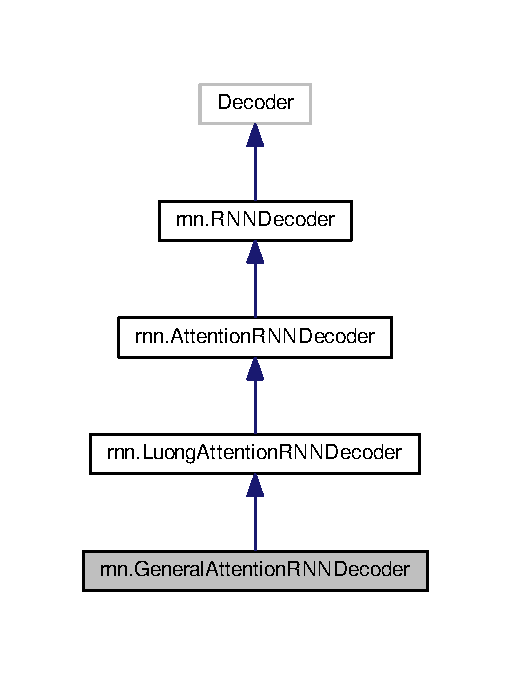
\includegraphics[width=245pt]{classrnn_1_1GeneralAttentionRNNDecoder__inherit__graph}
\end{center}
\end{figure}


Collaboration diagram for rnn.\+General\+Attention\+R\+N\+N\+Decoder\+:
\nopagebreak
\begin{figure}[H]
\begin{center}
\leavevmode
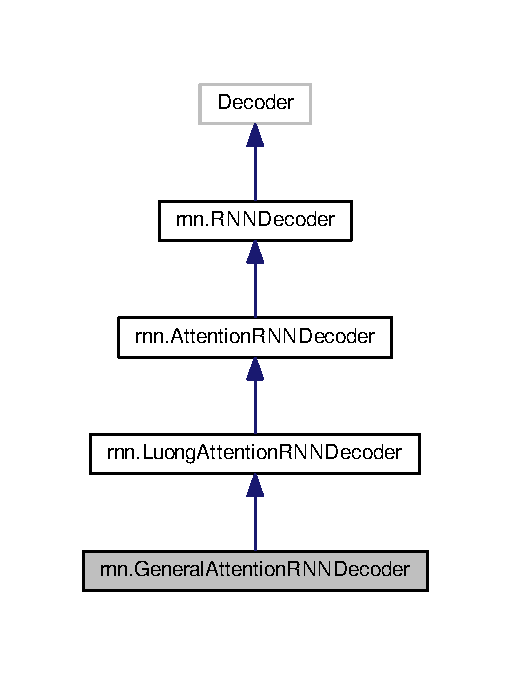
\includegraphics[width=245pt]{classrnn_1_1GeneralAttentionRNNDecoder__coll__graph}
\end{center}
\end{figure}
\subsection*{Public Member Functions}
\begin{DoxyCompactItemize}
\item 
def {\bfseries \+\_\+\+\_\+init\+\_\+\+\_\+}\hypertarget{classrnn_1_1GeneralAttentionRNNDecoder_ab29146b7be0f310e74af03e63fee5a0d}{}\label{classrnn_1_1GeneralAttentionRNNDecoder_ab29146b7be0f310e74af03e63fee5a0d}

\item 
def \hyperlink{classrnn_1_1GeneralAttentionRNNDecoder_a396d1ccba6f18aaadfb8cda1a8c2da95}{init\+\_\+parameters} (self)
\end{DoxyCompactItemize}
\subsection*{Static Public Attributes}
\begin{DoxyCompactItemize}
\item 
{\bfseries interface} = R\+N\+N\+Decoder.\+interface\hypertarget{classrnn_1_1GeneralAttentionRNNDecoder_aa2bca36c8dbcd5fa484c57327ccab46c}{}\label{classrnn_1_1GeneralAttentionRNNDecoder_aa2bca36c8dbcd5fa484c57327ccab46c}

\item 
bool {\bfseries abstract} = False\hypertarget{classrnn_1_1GeneralAttentionRNNDecoder_a3047fe7f55a476f80b964747c2dcf0b4}{}\label{classrnn_1_1GeneralAttentionRNNDecoder_a3047fe7f55a476f80b964747c2dcf0b4}

\end{DoxyCompactItemize}
\subsection*{Additional Inherited Members}


\subsection{Detailed Description}
\begin{DoxyVerb}Global attention mechanism for the recurrent decoder module. The algorithm is a specific case
of Luong style attention, where the scoring is based off of the linear activation
of the encoder output, and the dot product of the decoder hidden state with the result of the
activation from the linear layer.
\end{DoxyVerb}
 

\subsection{Member Function Documentation}
\index{rnn\+::\+General\+Attention\+R\+N\+N\+Decoder@{rnn\+::\+General\+Attention\+R\+N\+N\+Decoder}!init\+\_\+parameters@{init\+\_\+parameters}}
\index{init\+\_\+parameters@{init\+\_\+parameters}!rnn\+::\+General\+Attention\+R\+N\+N\+Decoder@{rnn\+::\+General\+Attention\+R\+N\+N\+Decoder}}
\subsubsection[{\texorpdfstring{init\+\_\+parameters(self)}{init_parameters(self)}}]{\setlength{\rightskip}{0pt plus 5cm}def rnn.\+General\+Attention\+R\+N\+N\+Decoder.\+init\+\_\+parameters (
\begin{DoxyParamCaption}
\item[{}]{self, }
\item[{}]{Decoder}
\end{DoxyParamCaption}
)}\hypertarget{classrnn_1_1GeneralAttentionRNNDecoder_a396d1ccba6f18aaadfb8cda1a8c2da95}{}\label{classrnn_1_1GeneralAttentionRNNDecoder_a396d1ccba6f18aaadfb8cda1a8c2da95}
\begin{DoxyVerb}Initializes the parameters for the decoder.
\end{DoxyVerb}
 

The documentation for this class was generated from the following file\+:\begin{DoxyCompactItemize}
\item 
src/components/decoders/rnn.\+py\end{DoxyCompactItemize}

\hypertarget{classreader_1_1InputPipeline}{}\section{reader.\+Input\+Pipeline Class Reference}
\label{classreader_1_1InputPipeline}\index{reader.\+Input\+Pipeline@{reader.\+Input\+Pipeline}}


Inheritance diagram for reader.\+Input\+Pipeline\+:
\nopagebreak
\begin{figure}[H]
\begin{center}
\leavevmode
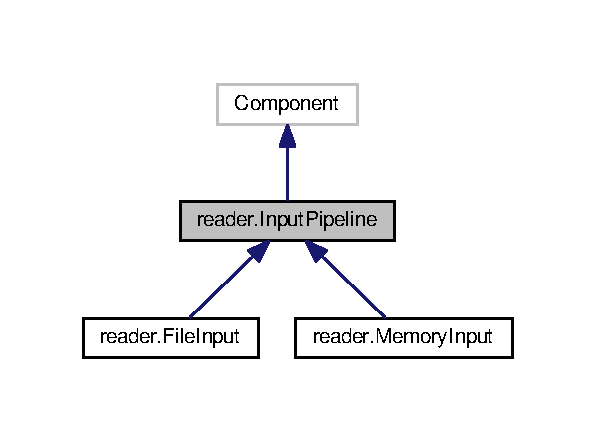
\includegraphics[width=286pt]{classreader_1_1InputPipeline__inherit__graph}
\end{center}
\end{figure}


Collaboration diagram for reader.\+Input\+Pipeline\+:
\nopagebreak
\begin{figure}[H]
\begin{center}
\leavevmode
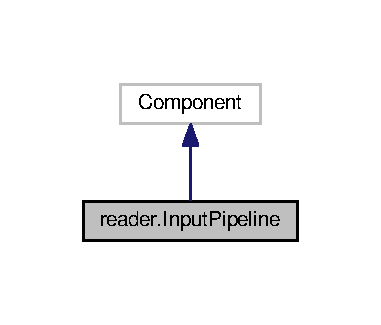
\includegraphics[width=183pt]{classreader_1_1InputPipeline__coll__graph}
\end{center}
\end{figure}
\subsection*{Public Member Functions}
\begin{DoxyCompactItemize}
\item 
def \hyperlink{classreader_1_1InputPipeline_af8d04604e1e29d9d9ad68d249e10e657}{batch\+\_\+generator} (self)
\end{DoxyCompactItemize}


\subsection{Detailed Description}
\begin{DoxyVerb}Derived classes should implement the reading logic for the seq2seq model. Readers divide the
data into segments. The purpose of this behaviour, is to keep the sentences with similar lengths
in segments, so they can be freely shuffled without mixing them together with larger sentences.
\end{DoxyVerb}
 

\subsection{Member Function Documentation}
\index{reader\+::\+Input\+Pipeline@{reader\+::\+Input\+Pipeline}!batch\+\_\+generator@{batch\+\_\+generator}}
\index{batch\+\_\+generator@{batch\+\_\+generator}!reader\+::\+Input\+Pipeline@{reader\+::\+Input\+Pipeline}}
\subsubsection[{\texorpdfstring{batch\+\_\+generator(self)}{batch_generator(self)}}]{\setlength{\rightskip}{0pt plus 5cm}def reader.\+Input\+Pipeline.\+batch\+\_\+generator (
\begin{DoxyParamCaption}
\item[{}]{self}
\end{DoxyParamCaption}
)}\hypertarget{classreader_1_1InputPipeline_af8d04604e1e29d9d9ad68d249e10e657}{}\label{classreader_1_1InputPipeline_af8d04604e1e29d9d9ad68d249e10e657}
\begin{DoxyVerb}The role of this function is to generate batches for the seq2seq model. The batch generation
should include the logic of shuffling the samples. A full iteration should include
all of the data samples.
\end{DoxyVerb}
 

The documentation for this class was generated from the following file\+:\begin{DoxyCompactItemize}
\item 
src/utils/reader.\+py\end{DoxyCompactItemize}

\hypertarget{classutils_1_1Interface}{}\section{utils.\+Interface Class Reference}
\label{classutils_1_1Interface}\index{utils.\+Interface@{utils.\+Interface}}
\subsection*{Public Member Functions}
\begin{DoxyCompactItemize}
\item 
def {\bfseries \+\_\+\+\_\+init\+\_\+\+\_\+} (self, kwargs)\hypertarget{classutils_1_1Interface_a8b95063a129db8d54005e05509bb10ef}{}\label{classutils_1_1Interface_a8b95063a129db8d54005e05509bb10ef}

\item 
def {\bfseries \+\_\+\+\_\+getitem\+\_\+\+\_\+} (self, key)\hypertarget{classutils_1_1Interface_a7b0232492feef2cd4e848dcc58e0f8c4}{}\label{classutils_1_1Interface_a7b0232492feef2cd4e848dcc58e0f8c4}

\item 
def {\bfseries \+\_\+\+\_\+next\+\_\+\+\_\+} (self)\hypertarget{classutils_1_1Interface_a62919668ead90f17fe08c88fdfb07e8f}{}\label{classutils_1_1Interface_a62919668ead90f17fe08c88fdfb07e8f}

\item 
def {\bfseries \+\_\+\+\_\+iter\+\_\+\+\_\+} (self)\hypertarget{classutils_1_1Interface_a504fdc18ad7d4ec0281d5b8b92061998}{}\label{classutils_1_1Interface_a504fdc18ad7d4ec0281d5b8b92061998}

\item 
def {\bfseries dictionary} (self)\hypertarget{classutils_1_1Interface_aa6384108e40c460afc316df970bccbe2}{}\label{classutils_1_1Interface_aa6384108e40c460afc316df970bccbe2}

\end{DoxyCompactItemize}
\subsection*{Static Public Member Functions}
\begin{DoxyCompactItemize}
\item 
def {\bfseries last\+\_\+key} (dictionary)\hypertarget{classutils_1_1Interface_abb5c706867e97a662b99c9ad82d52e98}{}\label{classutils_1_1Interface_abb5c706867e97a662b99c9ad82d52e98}

\end{DoxyCompactItemize}


The documentation for this class was generated from the following file\+:\begin{DoxyCompactItemize}
\item 
src/utils/utils.\+py\end{DoxyCompactItemize}

\hypertarget{classreader_1_1Language}{}\section{reader.\+Language Class Reference}
\label{classreader_1_1Language}\index{reader.\+Language@{reader.\+Language}}


Inheritance diagram for reader.\+Language\+:
\nopagebreak
\begin{figure}[H]
\begin{center}
\leavevmode
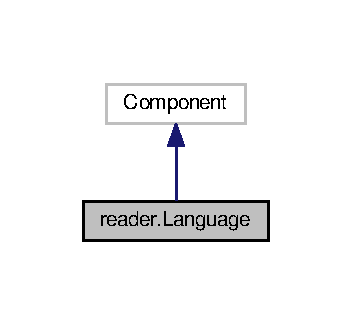
\includegraphics[width=169pt]{classreader_1_1Language__inherit__graph}
\end{center}
\end{figure}


Collaboration diagram for reader.\+Language\+:
\nopagebreak
\begin{figure}[H]
\begin{center}
\leavevmode
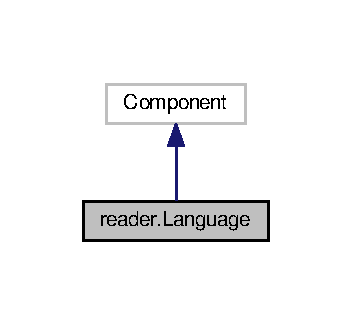
\includegraphics[width=169pt]{classreader_1_1Language__coll__graph}
\end{center}
\end{figure}
\subsection*{Public Member Functions}
\begin{DoxyCompactItemize}
\item 
def {\bfseries \+\_\+\+\_\+init\+\_\+\+\_\+}\hypertarget{classreader_1_1Language_a87c8088c36f415a49becda5c8a8f4f4a}{}\label{classreader_1_1Language_a87c8088c36f415a49becda5c8a8f4f4a}

\item 
def {\bfseries identifier} (self)\hypertarget{classreader_1_1Language_a94fbcfc6afd461253b63357051fcd415}{}\label{classreader_1_1Language_a94fbcfc6afd461253b63357051fcd415}

\item 
def {\bfseries input\+\_\+pipelines} (self)\hypertarget{classreader_1_1Language_af63b52231f647db16c3068f059b6b7cf}{}\label{classreader_1_1Language_af63b52231f647db16c3068f059b6b7cf}

\item 
def {\bfseries vocabulary} (self)\hypertarget{classreader_1_1Language_af8ce0fcb143b103f8ed8960ca29aa327}{}\label{classreader_1_1Language_af8ce0fcb143b103f8ed8960ca29aa327}

\end{DoxyCompactItemize}
\subsection*{Static Public Attributes}
\begin{DoxyCompactItemize}
\item 
bool {\bfseries abstract} = False\hypertarget{classreader_1_1Language_ae7b2a09ef605c3ea7317a22928af120d}{}\label{classreader_1_1Language_ae7b2a09ef605c3ea7317a22928af120d}

\item 
{\bfseries interface}
\end{DoxyCompactItemize}


\subsection{Detailed Description}
\begin{DoxyVerb}An abstract representation of ta language in an experiment. This class holds all relevant
information about a given language, its vocabulary, identifier and the corpus.
\end{DoxyVerb}
 

\subsection{Member Data Documentation}
\index{reader\+::\+Language@{reader\+::\+Language}!interface@{interface}}
\index{interface@{interface}!reader\+::\+Language@{reader\+::\+Language}}
\subsubsection[{\texorpdfstring{interface}{interface}}]{\setlength{\rightskip}{0pt plus 5cm}reader.\+Language.\+interface\hspace{0.3cm}{\ttfamily [static]}}\hypertarget{classreader_1_1Language_abb22a3a50e7636396663c49211fd97b3}{}\label{classreader_1_1Language_abb22a3a50e7636396663c49211fd97b3}
{\bfseries Initial value\+:}
\begin{DoxyCode}
1 = Interface(**\{
2         \textcolor{stringliteral}{'identifier'}:           (0, \textcolor{keywordtype}{None}),
3         \textcolor{stringliteral}{'vocabulary'}:           (1, Vocabulary),
4         \textcolor{stringliteral}{'input\_pipelines'}:      (2, InputPipeline),
5     \})
\end{DoxyCode}


The documentation for this class was generated from the following file\+:\begin{DoxyCompactItemize}
\item 
src/utils/reader.\+py\end{DoxyCompactItemize}

\hypertarget{classanalysis_1_1LatentStateData}{}\section{analysis.\+Latent\+State\+Data Class Reference}
\label{classanalysis_1_1LatentStateData}\index{analysis.\+Latent\+State\+Data@{analysis.\+Latent\+State\+Data}}


Inheritance diagram for analysis.\+Latent\+State\+Data\+:
\nopagebreak
\begin{figure}[H]
\begin{center}
\leavevmode
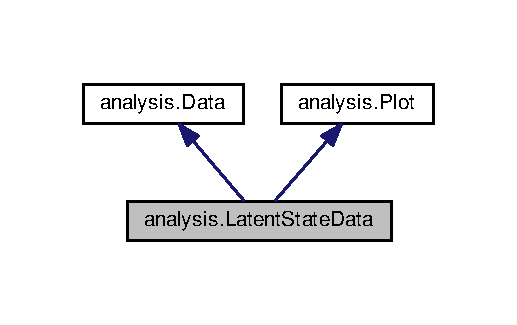
\includegraphics[width=248pt]{classanalysis_1_1LatentStateData__inherit__graph}
\end{center}
\end{figure}


Collaboration diagram for analysis.\+Latent\+State\+Data\+:
\nopagebreak
\begin{figure}[H]
\begin{center}
\leavevmode
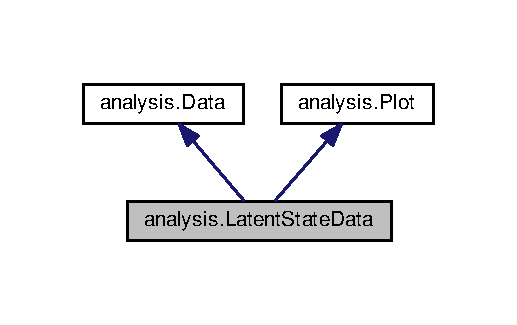
\includegraphics[width=248pt]{classanalysis_1_1LatentStateData__coll__graph}
\end{center}
\end{figure}
\subsection*{Public Member Functions}
\begin{DoxyCompactItemize}
\item 
def {\bfseries \+\_\+\+\_\+init\+\_\+\+\_\+} (self)\hypertarget{classanalysis_1_1LatentStateData_ae0c63041952aeeee67a23ed3810f58cf}{}\label{classanalysis_1_1LatentStateData_ae0c63041952aeeee67a23ed3810f58cf}

\item 
def {\bfseries add} (self, identifier, value)\hypertarget{classanalysis_1_1LatentStateData_abe6ae250f7eb3e9304028802fafd7f95}{}\label{classanalysis_1_1LatentStateData_abe6ae250f7eb3e9304028802fafd7f95}

\item 
def {\bfseries get\+\_\+required\+\_\+keys} (self)\hypertarget{classanalysis_1_1LatentStateData_a95d8c3a35253120463d77c2a1931b45e}{}\label{classanalysis_1_1LatentStateData_a95d8c3a35253120463d77c2a1931b45e}

\end{DoxyCompactItemize}
\subsection*{Static Public Member Functions}
\begin{DoxyCompactItemize}
\item 
def {\bfseries display} (data, plot\+\_\+size, epochs, epoch\+\_\+range, identifiers=None, params)\hypertarget{classanalysis_1_1LatentStateData_a037196cb9796998eac40d664c1a1788f}{}\label{classanalysis_1_1LatentStateData_a037196cb9796998eac40d664c1a1788f}

\end{DoxyCompactItemize}
\subsection*{Additional Inherited Members}


\subsection{Detailed Description}
\begin{DoxyVerb}\end{DoxyVerb}
 

The documentation for this class was generated from the following file\+:\begin{DoxyCompactItemize}
\item 
src/utils/analysis.\+py\end{DoxyCompactItemize}

\hypertarget{classutils_1_1Layer}{}\section{utils.\+Layer Class Reference}
\label{classutils_1_1Layer}\index{utils.\+Layer@{utils.\+Layer}}


Inheritance diagram for utils.\+Layer\+:
\nopagebreak
\begin{figure}[H]
\begin{center}
\leavevmode
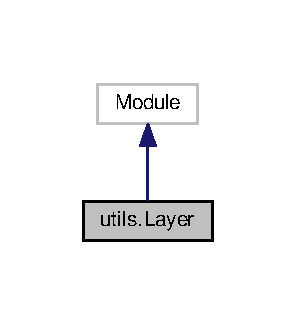
\includegraphics[width=142pt]{classutils_1_1Layer__inherit__graph}
\end{center}
\end{figure}


Collaboration diagram for utils.\+Layer\+:
\nopagebreak
\begin{figure}[H]
\begin{center}
\leavevmode
\includegraphics[width=142pt]{classutils_1_1Layer__coll__graph}
\end{center}
\end{figure}
\subsection*{Public Member Functions}
\begin{DoxyCompactItemize}
\item 
def \hyperlink{classutils_1_1Layer_a8b1a990e121e91650bf3e72c4ab5596b}{\+\_\+\+\_\+init\+\_\+\+\_\+} (self, input\+\_\+size, output\+\_\+size, use\+\_\+cuda)
\item 
def \hyperlink{classutils_1_1Layer_aeb83b870a8f03ff4767e0cc5e0c61d10}{forward} (self, inputs)
\item 
def {\bfseries freeze} (self)\hypertarget{classutils_1_1Layer_ae4a853f74ca32dc1ae90b50165e42644}{}\label{classutils_1_1Layer_ae4a853f74ca32dc1ae90b50165e42644}

\item 
def {\bfseries unfreeze} (self)\hypertarget{classutils_1_1Layer_a9384f978f727be33aa016f82bd99222d}{}\label{classutils_1_1Layer_a9384f978f727be33aa016f82bd99222d}

\item 
def \hyperlink{classutils_1_1Layer_ac73933ab4370267401d2ba827603f03b}{optimizer} (self)
\item 
def \hyperlink{classutils_1_1Layer_ac10a658fba9398e741d6fe5dd8bf34c5}{state} (self)
\item 
def \hyperlink{classutils_1_1Layer_a75d4bad3c8ebcc4f3b76e3c4cd44bf8b}{state} (self, states)
\end{DoxyCompactItemize}
\subsection*{Public Attributes}
\begin{DoxyCompactItemize}
\item 
{\bfseries size}\hypertarget{classutils_1_1Layer_a7d69c224205d9a98b933b2ee6faae039}{}\label{classutils_1_1Layer_a7d69c224205d9a98b933b2ee6faae039}

\end{DoxyCompactItemize}


\subsection{Constructor \& Destructor Documentation}
\index{utils\+::\+Layer@{utils\+::\+Layer}!\+\_\+\+\_\+init\+\_\+\+\_\+@{\+\_\+\+\_\+init\+\_\+\+\_\+}}
\index{\+\_\+\+\_\+init\+\_\+\+\_\+@{\+\_\+\+\_\+init\+\_\+\+\_\+}!utils\+::\+Layer@{utils\+::\+Layer}}
\subsubsection[{\texorpdfstring{\+\_\+\+\_\+init\+\_\+\+\_\+(self, input\+\_\+size, output\+\_\+size, use\+\_\+cuda)}{__init__(self, input_size, output_size, use_cuda)}}]{\setlength{\rightskip}{0pt plus 5cm}def utils.\+Layer.\+\_\+\+\_\+init\+\_\+\+\_\+ (
\begin{DoxyParamCaption}
\item[{}]{self, }
\item[{}]{input\+\_\+size, }
\item[{}]{output\+\_\+size, }
\item[{}]{use\+\_\+cuda}
\end{DoxyParamCaption}
)}\hypertarget{classutils_1_1Layer_a8b1a990e121e91650bf3e72c4ab5596b}{}\label{classutils_1_1Layer_a8b1a990e121e91650bf3e72c4ab5596b}
\begin{DoxyVerb}:param input_size:

:param output_size:

:param use_cuda:\end{DoxyVerb}
 

\subsection{Member Function Documentation}
\index{utils\+::\+Layer@{utils\+::\+Layer}!forward@{forward}}
\index{forward@{forward}!utils\+::\+Layer@{utils\+::\+Layer}}
\subsubsection[{\texorpdfstring{forward(self, inputs)}{forward(self, inputs)}}]{\setlength{\rightskip}{0pt plus 5cm}def utils.\+Layer.\+forward (
\begin{DoxyParamCaption}
\item[{}]{self, }
\item[{}]{inputs}
\end{DoxyParamCaption}
)}\hypertarget{classutils_1_1Layer_aeb83b870a8f03ff4767e0cc5e0c61d10}{}\label{classutils_1_1Layer_aeb83b870a8f03ff4767e0cc5e0c61d10}
\begin{DoxyVerb}:param inputs:

:return outputs:\end{DoxyVerb}
 \index{utils\+::\+Layer@{utils\+::\+Layer}!optimizer@{optimizer}}
\index{optimizer@{optimizer}!utils\+::\+Layer@{utils\+::\+Layer}}
\subsubsection[{\texorpdfstring{optimizer(self)}{optimizer(self)}}]{\setlength{\rightskip}{0pt plus 5cm}def utils.\+Layer.\+optimizer (
\begin{DoxyParamCaption}
\item[{}]{self}
\end{DoxyParamCaption}
)}\hypertarget{classutils_1_1Layer_ac73933ab4370267401d2ba827603f03b}{}\label{classutils_1_1Layer_ac73933ab4370267401d2ba827603f03b}
\begin{DoxyVerb}Property for the optimizer of the layer.
\end{DoxyVerb}
 \index{utils\+::\+Layer@{utils\+::\+Layer}!state@{state}}
\index{state@{state}!utils\+::\+Layer@{utils\+::\+Layer}}
\subsubsection[{\texorpdfstring{state(self)}{state(self)}}]{\setlength{\rightskip}{0pt plus 5cm}def utils.\+Layer.\+state (
\begin{DoxyParamCaption}
\item[{}]{self}
\end{DoxyParamCaption}
)}\hypertarget{classutils_1_1Layer_ac10a658fba9398e741d6fe5dd8bf34c5}{}\label{classutils_1_1Layer_ac10a658fba9398e741d6fe5dd8bf34c5}
\begin{DoxyVerb}Property for the state of the embedding.
\end{DoxyVerb}
 \index{utils\+::\+Layer@{utils\+::\+Layer}!state@{state}}
\index{state@{state}!utils\+::\+Layer@{utils\+::\+Layer}}
\subsubsection[{\texorpdfstring{state(self, states)}{state(self, states)}}]{\setlength{\rightskip}{0pt plus 5cm}def utils.\+Layer.\+state (
\begin{DoxyParamCaption}
\item[{}]{self, }
\item[{}]{states}
\end{DoxyParamCaption}
)}\hypertarget{classutils_1_1Layer_a75d4bad3c8ebcc4f3b76e3c4cd44bf8b}{}\label{classutils_1_1Layer_a75d4bad3c8ebcc4f3b76e3c4cd44bf8b}
\begin{DoxyVerb}Setter method for the state of the embedding.
:param states: dict, containing the state of the weights and optimizer.
\end{DoxyVerb}
 

The documentation for this class was generated from the following file\+:\begin{DoxyCompactItemize}
\item 
src/components/utils/utils.\+py\end{DoxyCompactItemize}

\hypertarget{classutils_1_1Logger}{}\section{utils.\+Logger Class Reference}
\label{classutils_1_1Logger}\index{utils.\+Logger@{utils.\+Logger}}
\subsection*{Public Member Functions}
\begin{DoxyCompactItemize}
\item 
def \hyperlink{classutils_1_1Logger_aaf70454f806ae064f4289a7133f6941d}{\+\_\+\+\_\+init\+\_\+\+\_\+} (self, params, dump\+\_\+interval=1000)
\item 
def \hyperlink{classutils_1_1Logger_ae36b75f351b406c7ddec930d1de69768}{\+\_\+\+\_\+call\+\_\+\+\_\+} (self, args, func, kwargs)
\item 
def \hyperlink{classutils_1_1Logger_aa9f043a740d882bb41830624208b79c5}{log\+\_\+dir} (self)
\item 
def \hyperlink{classutils_1_1Logger_a7c8306f54af28a9585a41d0cd0629984}{log\+\_\+dir} (self, log\+\_\+dir)
\end{DoxyCompactItemize}


\subsection{Detailed Description}
\begin{DoxyVerb}Logger class for saving the progress of training.
\end{DoxyVerb}
 

\subsection{Constructor \& Destructor Documentation}
\index{utils\+::\+Logger@{utils\+::\+Logger}!\+\_\+\+\_\+init\+\_\+\+\_\+@{\+\_\+\+\_\+init\+\_\+\+\_\+}}
\index{\+\_\+\+\_\+init\+\_\+\+\_\+@{\+\_\+\+\_\+init\+\_\+\+\_\+}!utils\+::\+Logger@{utils\+::\+Logger}}
\subsubsection[{\texorpdfstring{\+\_\+\+\_\+init\+\_\+\+\_\+(self, params, dump\+\_\+interval=1000)}{__init__(self, params, dump_interval=1000)}}]{\setlength{\rightskip}{0pt plus 5cm}def utils.\+Logger.\+\_\+\+\_\+init\+\_\+\+\_\+ (
\begin{DoxyParamCaption}
\item[{}]{self, }
\item[{}]{params, }
\item[{}]{dump\+\_\+interval = {\ttfamily 1000}}
\end{DoxyParamCaption}
)}\hypertarget{classutils_1_1Logger_aaf70454f806ae064f4289a7133f6941d}{}\label{classutils_1_1Logger_aaf70454f806ae064f4289a7133f6941d}
\begin{DoxyVerb}A logger instance. Instantiation should happen as a parameter of logging decorator.
:param params: tuple, name of the input parameters, which will be logged.
:param dump_interval: int, number of iteration, between two log dumps.
\end{DoxyVerb}
 

\subsection{Member Function Documentation}
\index{utils\+::\+Logger@{utils\+::\+Logger}!\+\_\+\+\_\+call\+\_\+\+\_\+@{\+\_\+\+\_\+call\+\_\+\+\_\+}}
\index{\+\_\+\+\_\+call\+\_\+\+\_\+@{\+\_\+\+\_\+call\+\_\+\+\_\+}!utils\+::\+Logger@{utils\+::\+Logger}}
\subsubsection[{\texorpdfstring{\+\_\+\+\_\+call\+\_\+\+\_\+(self, args, func, kwargs)}{__call__(self, args, func, kwargs)}}]{\setlength{\rightskip}{0pt plus 5cm}def utils.\+Logger.\+\_\+\+\_\+call\+\_\+\+\_\+ (
\begin{DoxyParamCaption}
\item[{}]{self, }
\item[{}]{args, }
\item[{}]{func, }
\item[{}]{kwargs}
\end{DoxyParamCaption}
)}\hypertarget{classutils_1_1Logger_ae36b75f351b406c7ddec930d1de69768}{}\label{classutils_1_1Logger_ae36b75f351b406c7ddec930d1de69768}
\begin{DoxyVerb}Invocation of a logger object will execute the given function, record the time required
for this operation, and then save the results and given input parameters to the log dictionary.
:param args: arguments of the function, which will be executed.
:param func: function to be executed.
:param kwargs: keyword arguments of the function to be executed.
:return: result of the execution.
\end{DoxyVerb}
 \index{utils\+::\+Logger@{utils\+::\+Logger}!log\+\_\+dir@{log\+\_\+dir}}
\index{log\+\_\+dir@{log\+\_\+dir}!utils\+::\+Logger@{utils\+::\+Logger}}
\subsubsection[{\texorpdfstring{log\+\_\+dir(self)}{log_dir(self)}}]{\setlength{\rightskip}{0pt plus 5cm}def utils.\+Logger.\+log\+\_\+dir (
\begin{DoxyParamCaption}
\item[{}]{self}
\end{DoxyParamCaption}
)}\hypertarget{classutils_1_1Logger_aa9f043a740d882bb41830624208b79c5}{}\label{classutils_1_1Logger_aa9f043a740d882bb41830624208b79c5}
\begin{DoxyVerb}Property for the logging directory.
:return: str, location of the logs.
\end{DoxyVerb}
 \index{utils\+::\+Logger@{utils\+::\+Logger}!log\+\_\+dir@{log\+\_\+dir}}
\index{log\+\_\+dir@{log\+\_\+dir}!utils\+::\+Logger@{utils\+::\+Logger}}
\subsubsection[{\texorpdfstring{log\+\_\+dir(self, log\+\_\+dir)}{log_dir(self, log_dir)}}]{\setlength{\rightskip}{0pt plus 5cm}def utils.\+Logger.\+log\+\_\+dir (
\begin{DoxyParamCaption}
\item[{}]{self, }
\item[{}]{log\+\_\+dir}
\end{DoxyParamCaption}
)}\hypertarget{classutils_1_1Logger_a7c8306f54af28a9585a41d0cd0629984}{}\label{classutils_1_1Logger_a7c8306f54af28a9585a41d0cd0629984}
\begin{DoxyVerb}Setter for the directory of the logging directory.
\end{DoxyVerb}
 

The documentation for this class was generated from the following file\+:\begin{DoxyCompactItemize}
\item 
src/utils/utils.\+py\end{DoxyCompactItemize}

\hypertarget{classrnn_1_1LuongAttentionRNNDecoder}{}\section{rnn.\+Luong\+Attention\+R\+N\+N\+Decoder Class Reference}
\label{classrnn_1_1LuongAttentionRNNDecoder}\index{rnn.\+Luong\+Attention\+R\+N\+N\+Decoder@{rnn.\+Luong\+Attention\+R\+N\+N\+Decoder}}


Inheritance diagram for rnn.\+Luong\+Attention\+R\+N\+N\+Decoder\+:
\nopagebreak
\begin{figure}[H]
\begin{center}
\leavevmode
\includegraphics[width=350pt]{classrnn_1_1LuongAttentionRNNDecoder__inherit__graph}
\end{center}
\end{figure}


Collaboration diagram for rnn.\+Luong\+Attention\+R\+N\+N\+Decoder\+:
\nopagebreak
\begin{figure}[H]
\begin{center}
\leavevmode
\includegraphics[width=238pt]{classrnn_1_1LuongAttentionRNNDecoder__coll__graph}
\end{center}
\end{figure}
\subsection*{Public Member Functions}
\begin{DoxyCompactItemize}
\item 
def {\bfseries \+\_\+\+\_\+init\+\_\+\+\_\+}\hypertarget{classrnn_1_1LuongAttentionRNNDecoder_adb0e81a64d832a59a658bf7980c6b0d9}{}\label{classrnn_1_1LuongAttentionRNNDecoder_adb0e81a64d832a59a658bf7980c6b0d9}

\item 
def \hyperlink{classrnn_1_1LuongAttentionRNNDecoder_a83e3361b531de2b9cbf2a6d775b6a350}{init\+\_\+parameters} (self)
\end{DoxyCompactItemize}
\subsection*{Additional Inherited Members}


\subsection{Detailed Description}
\begin{DoxyVerb}Attention mechanism for the recurrent decoder module. The algorithm is based on:

    https://arxiv.org/pdf/1508.04025.pdf

The computational path of the method differs from the Bahdanau style, since
here the context vector contributes to the calculation of the hidden state, after the
computations of the recurrent layer.

    h(t) -> a(t) -> c(t) -> h*(t)\end{DoxyVerb}
 

\subsection{Member Function Documentation}
\index{rnn\+::\+Luong\+Attention\+R\+N\+N\+Decoder@{rnn\+::\+Luong\+Attention\+R\+N\+N\+Decoder}!init\+\_\+parameters@{init\+\_\+parameters}}
\index{init\+\_\+parameters@{init\+\_\+parameters}!rnn\+::\+Luong\+Attention\+R\+N\+N\+Decoder@{rnn\+::\+Luong\+Attention\+R\+N\+N\+Decoder}}
\subsubsection[{\texorpdfstring{init\+\_\+parameters(self)}{init_parameters(self)}}]{\setlength{\rightskip}{0pt plus 5cm}def rnn.\+Luong\+Attention\+R\+N\+N\+Decoder.\+init\+\_\+parameters (
\begin{DoxyParamCaption}
\item[{}]{self, }
\item[{}]{Decoder}
\end{DoxyParamCaption}
)}\hypertarget{classrnn_1_1LuongAttentionRNNDecoder_a83e3361b531de2b9cbf2a6d775b6a350}{}\label{classrnn_1_1LuongAttentionRNNDecoder_a83e3361b531de2b9cbf2a6d775b6a350}
\begin{DoxyVerb}Initializes the parameters for the decoder.
\end{DoxyVerb}
 

The documentation for this class was generated from the following file\+:\begin{DoxyCompactItemize}
\item 
src/components/decoders/rnn.\+py\end{DoxyCompactItemize}

\hypertarget{classreader_1_1MemoryInput}{}\section{reader.\+Memory\+Input Class Reference}
\label{classreader_1_1MemoryInput}\index{reader.\+Memory\+Input@{reader.\+Memory\+Input}}


Inheritance diagram for reader.\+Memory\+Input\+:
\nopagebreak
\begin{figure}[H]
\begin{center}
\leavevmode
\includegraphics[width=184pt]{classreader_1_1MemoryInput__inherit__graph}
\end{center}
\end{figure}


Collaboration diagram for reader.\+Memory\+Input\+:
\nopagebreak
\begin{figure}[H]
\begin{center}
\leavevmode
\includegraphics[width=184pt]{classreader_1_1MemoryInput__coll__graph}
\end{center}
\end{figure}
\subsection*{Public Member Functions}
\begin{DoxyCompactItemize}
\item 
def {\bfseries \+\_\+\+\_\+init\+\_\+\+\_\+}\hypertarget{classreader_1_1MemoryInput_a5e90c1e76caf2286e50fb47cfbdb47d9}{}\label{classreader_1_1MemoryInput_a5e90c1e76caf2286e50fb47cfbdb47d9}

\item 
def \hyperlink{classreader_1_1MemoryInput_ae081cdff2fd546cae6cc05f52eb1c7a7}{batch\+\_\+generator} (self)
\item 
def \hyperlink{classreader_1_1MemoryInput_a56635971dedfb9830885abc7e8158feb}{print\+\_\+validation\+\_\+format} (self, dictionary)
\item 
def \hyperlink{classreader_1_1MemoryInput_a57b5d5e3039725ca9a84cecdd0b66051}{corpora} (self)
\item 
def \hyperlink{classreader_1_1MemoryInput_a4fec72e8b1f438ed2f2c733fa65c5577}{vocabulary} (self)
\item 
def {\bfseries batch\+\_\+size} (self)\hypertarget{classreader_1_1MemoryInput_a4a37a8c307159adc280eabbf78521978}{}\label{classreader_1_1MemoryInput_a4a37a8c307159adc280eabbf78521978}

\end{DoxyCompactItemize}
\subsection*{Static Public Attributes}
\begin{DoxyCompactItemize}
\item 
{\bfseries interface}
\item 
bool {\bfseries abstract} = False\hypertarget{classreader_1_1MemoryInput_a71d03d985f949d8878ae0ec734d1a2b8}{}\label{classreader_1_1MemoryInput_a71d03d985f949d8878ae0ec734d1a2b8}

\end{DoxyCompactItemize}


\subsection{Detailed Description}
\begin{DoxyVerb}A faster implementation of reader class than FileReader. The source data is fully loaded into
the memory.
\end{DoxyVerb}
 

\subsection{Member Function Documentation}
\index{reader\+::\+Memory\+Input@{reader\+::\+Memory\+Input}!batch\+\_\+generator@{batch\+\_\+generator}}
\index{batch\+\_\+generator@{batch\+\_\+generator}!reader\+::\+Memory\+Input@{reader\+::\+Memory\+Input}}
\subsubsection[{\texorpdfstring{batch\+\_\+generator(self)}{batch_generator(self)}}]{\setlength{\rightskip}{0pt plus 5cm}def reader.\+Memory\+Input.\+batch\+\_\+generator (
\begin{DoxyParamCaption}
\item[{}]{self}
\end{DoxyParamCaption}
)}\hypertarget{classreader_1_1MemoryInput_ae081cdff2fd546cae6cc05f52eb1c7a7}{}\label{classreader_1_1MemoryInput_ae081cdff2fd546cae6cc05f52eb1c7a7}
\begin{DoxyVerb}Generator for mini-batches. Data is read from memory. The _format_batch function comes from the
definition of the task. It is a wrapper function that transform the generated batch of data into a form,
that is convenient for the current task.

:return:
    tuple, a PyTorch Variable of dimension (Batch_size, Sequence_length), containing
    the ids of words, sorted by their length in descending order. Each sample is
    padded to the length of the longest sequence in the batch/segment.
    The latter behaviour may vary. Second element of the tuple is a numpy array
    of the lengths of the original sequences (without padding).
\end{DoxyVerb}
 \index{reader\+::\+Memory\+Input@{reader\+::\+Memory\+Input}!corpora@{corpora}}
\index{corpora@{corpora}!reader\+::\+Memory\+Input@{reader\+::\+Memory\+Input}}
\subsubsection[{\texorpdfstring{corpora(self)}{corpora(self)}}]{\setlength{\rightskip}{0pt plus 5cm}def reader.\+Memory\+Input.\+corpora (
\begin{DoxyParamCaption}
\item[{}]{self}
\end{DoxyParamCaption}
)}\hypertarget{classreader_1_1MemoryInput_a57b5d5e3039725ca9a84cecdd0b66051}{}\label{classreader_1_1MemoryInput_a57b5d5e3039725ca9a84cecdd0b66051}
\begin{DoxyVerb}Property for the corpora of the reader.
\end{DoxyVerb}
 \index{reader\+::\+Memory\+Input@{reader\+::\+Memory\+Input}!print\+\_\+validation\+\_\+format@{print\+\_\+validation\+\_\+format}}
\index{print\+\_\+validation\+\_\+format@{print\+\_\+validation\+\_\+format}!reader\+::\+Memory\+Input@{reader\+::\+Memory\+Input}}
\subsubsection[{\texorpdfstring{print\+\_\+validation\+\_\+format(self, dictionary)}{print_validation_format(self, dictionary)}}]{\setlength{\rightskip}{0pt plus 5cm}def reader.\+Memory\+Input.\+print\+\_\+validation\+\_\+format (
\begin{DoxyParamCaption}
\item[{}]{self, }
\item[{}]{dictionary}
\end{DoxyParamCaption}
)}\hypertarget{classreader_1_1MemoryInput_a56635971dedfb9830885abc7e8158feb}{}\label{classreader_1_1MemoryInput_a56635971dedfb9830885abc7e8158feb}
\begin{DoxyVerb}Convenience function for printing the parameters of the function, to the standard output.
The parameters must be provided as keyword arguments. Each argument must contain a 2D
array containing word ids, which will be converted to the represented words from the
dictionary of the language, used by the reader instance.
\end{DoxyVerb}
 \index{reader\+::\+Memory\+Input@{reader\+::\+Memory\+Input}!vocabulary@{vocabulary}}
\index{vocabulary@{vocabulary}!reader\+::\+Memory\+Input@{reader\+::\+Memory\+Input}}
\subsubsection[{\texorpdfstring{vocabulary(self)}{vocabulary(self)}}]{\setlength{\rightskip}{0pt plus 5cm}def reader.\+Memory\+Input.\+vocabulary (
\begin{DoxyParamCaption}
\item[{}]{self}
\end{DoxyParamCaption}
)}\hypertarget{classreader_1_1MemoryInput_a4fec72e8b1f438ed2f2c733fa65c5577}{}\label{classreader_1_1MemoryInput_a4fec72e8b1f438ed2f2c733fa65c5577}
\begin{DoxyVerb}Property for the reader object's vocabulary.
\end{DoxyVerb}
 

\subsection{Member Data Documentation}
\index{reader\+::\+Memory\+Input@{reader\+::\+Memory\+Input}!interface@{interface}}
\index{interface@{interface}!reader\+::\+Memory\+Input@{reader\+::\+Memory\+Input}}
\subsubsection[{\texorpdfstring{interface}{interface}}]{\setlength{\rightskip}{0pt plus 5cm}reader.\+Memory\+Input.\+interface\hspace{0.3cm}{\ttfamily [static]}}\hypertarget{classreader_1_1MemoryInput_a2adda01eeff537baa14a0a0f47c3bb37}{}\label{classreader_1_1MemoryInput_a2adda01eeff537baa14a0a0f47c3bb37}
{\bfseries Initial value\+:}
\begin{DoxyCode}
1 = Interface(**\{
2         \textcolor{stringliteral}{'max\_segment\_size'}:  (0, \textcolor{keywordtype}{None}),
3         \textcolor{stringliteral}{'batch\_size'}:        (1, \textcolor{keywordtype}{None}),
4         \textcolor{stringliteral}{'padding\_type'}:      (2, \textcolor{keywordtype}{None}),
5         \textcolor{stringliteral}{'shuffle'}:           (3, \textcolor{keywordtype}{None}),
6         \textcolor{stringliteral}{'cuda'}:              (4, \textcolor{stringliteral}{'Experiment:Policy:cuda$'}),
7         \textcolor{stringliteral}{'corpora'}:           (5, Corpora)
8     \})
\end{DoxyCode}


The documentation for this class was generated from the following file\+:\begin{DoxyCompactItemize}
\item 
src/utils/reader.\+py\end{DoxyCompactItemize}

\hypertarget{classexperiments_1_1MergedCurriculumTranslation}{}\section{experiments.\+Merged\+Curriculum\+Translation Class Reference}
\label{classexperiments_1_1MergedCurriculumTranslation}\index{experiments.\+Merged\+Curriculum\+Translation@{experiments.\+Merged\+Curriculum\+Translation}}


Inheritance diagram for experiments.\+Merged\+Curriculum\+Translation\+:
\nopagebreak
\begin{figure}[H]
\begin{center}
\leavevmode
\includegraphics[width=232pt]{classexperiments_1_1MergedCurriculumTranslation__inherit__graph}
\end{center}
\end{figure}


Collaboration diagram for experiments.\+Merged\+Curriculum\+Translation\+:
\nopagebreak
\begin{figure}[H]
\begin{center}
\leavevmode
\includegraphics[width=232pt]{classexperiments_1_1MergedCurriculumTranslation__coll__graph}
\end{center}
\end{figure}
\subsection*{Public Member Functions}
\begin{DoxyCompactItemize}
\item 
def {\bfseries \+\_\+\+\_\+init\+\_\+\+\_\+}\hypertarget{classexperiments_1_1MergedCurriculumTranslation_a9f2daa6e845b3562097c224c57a7b752}{}\label{classexperiments_1_1MergedCurriculumTranslation_a9f2daa6e845b3562097c224c57a7b752}

\item 
def {\bfseries train}\hypertarget{classexperiments_1_1MergedCurriculumTranslation_a05c0be7c2ed4a43cb84409c336f2a43f}{}\label{classexperiments_1_1MergedCurriculumTranslation_a05c0be7c2ed4a43cb84409c336f2a43f}

\item 
def \hyperlink{classexperiments_1_1MergedCurriculumTranslation_ad0f290d29438846fce55e6fcca7d135b}{validate} (self)
\item 
def \hyperlink{classexperiments_1_1MergedCurriculumTranslation_a965ce3d442924c0c92999e76d2cc744f}{test} (self)
\item 
def \hyperlink{classexperiments_1_1MergedCurriculumTranslation_aaa6b0b958add43289836e072d79eff5b}{evaluate} (self)
\item 
def \hyperlink{classexperiments_1_1MergedCurriculumTranslation_acc0cb9dfc9e83e461d64aca96046c592}{state} (self)
\item 
def \hyperlink{classexperiments_1_1MergedCurriculumTranslation_a5dd0db1db771158f5baa8faafd78fd03}{state} (self, state)
\end{DoxyCompactItemize}
\subsection*{Public Attributes}
\begin{DoxyCompactItemize}
\item 
{\bfseries reguralize}\hypertarget{classexperiments_1_1MergedCurriculumTranslation_aae8aeee74af48c305f482acfe7f08c57}{}\label{classexperiments_1_1MergedCurriculumTranslation_aae8aeee74af48c305f482acfe7f08c57}

\end{DoxyCompactItemize}
\subsection*{Static Public Attributes}
\begin{DoxyCompactItemize}
\item 
{\bfseries interface} = Unsupervised\+Translation.\+interface\hypertarget{classexperiments_1_1MergedCurriculumTranslation_ae45acf0b47e0a61e43936c7c40568f4e}{}\label{classexperiments_1_1MergedCurriculumTranslation_ae45acf0b47e0a61e43936c7c40568f4e}

\item 
bool {\bfseries abstract} = False\hypertarget{classexperiments_1_1MergedCurriculumTranslation_a33f79d34a935056931595267684513a6}{}\label{classexperiments_1_1MergedCurriculumTranslation_a33f79d34a935056931595267684513a6}

\end{DoxyCompactItemize}
\subsection*{Additional Inherited Members}


\subsection{Detailed Description}
\begin{DoxyVerb}\end{DoxyVerb}
 

\subsection{Member Function Documentation}
\index{experiments\+::\+Merged\+Curriculum\+Translation@{experiments\+::\+Merged\+Curriculum\+Translation}!evaluate@{evaluate}}
\index{evaluate@{evaluate}!experiments\+::\+Merged\+Curriculum\+Translation@{experiments\+::\+Merged\+Curriculum\+Translation}}
\subsubsection[{\texorpdfstring{evaluate(self)}{evaluate(self)}}]{\setlength{\rightskip}{0pt plus 5cm}def experiments.\+Merged\+Curriculum\+Translation.\+evaluate (
\begin{DoxyParamCaption}
\item[{}]{self, }
\item[{}]{dict}
\end{DoxyParamCaption}
)}\hypertarget{classexperiments_1_1MergedCurriculumTranslation_aaa6b0b958add43289836e072d79eff5b}{}\label{classexperiments_1_1MergedCurriculumTranslation_aaa6b0b958add43289836e072d79eff5b}
\begin{DoxyVerb}This function evaluates the model. Input data is propagated forward, and then the loss calculated
based on the same loss function which was used during training. The weights however, are not modified
in this function.

:return logs:
    A list of DataLog type objects, that contain the logging data for the languages. The number of
    data logs equal to the number of languages, and each data log contains information about the
    produced output for the whole data set of a language.

    Additional outputs depend on the chosen model.
\end{DoxyVerb}
 \index{experiments\+::\+Merged\+Curriculum\+Translation@{experiments\+::\+Merged\+Curriculum\+Translation}!state@{state}}
\index{state@{state}!experiments\+::\+Merged\+Curriculum\+Translation@{experiments\+::\+Merged\+Curriculum\+Translation}}
\subsubsection[{\texorpdfstring{state(self)}{state(self)}}]{\setlength{\rightskip}{0pt plus 5cm}def experiments.\+Merged\+Curriculum\+Translation.\+state (
\begin{DoxyParamCaption}
\item[{}]{self}
\end{DoxyParamCaption}
)}\hypertarget{classexperiments_1_1MergedCurriculumTranslation_acc0cb9dfc9e83e461d64aca96046c592}{}\label{classexperiments_1_1MergedCurriculumTranslation_acc0cb9dfc9e83e461d64aca96046c592}
\begin{DoxyVerb}Property for the state of the task.
\end{DoxyVerb}
 \index{experiments\+::\+Merged\+Curriculum\+Translation@{experiments\+::\+Merged\+Curriculum\+Translation}!state@{state}}
\index{state@{state}!experiments\+::\+Merged\+Curriculum\+Translation@{experiments\+::\+Merged\+Curriculum\+Translation}}
\subsubsection[{\texorpdfstring{state(self, state)}{state(self, state)}}]{\setlength{\rightskip}{0pt plus 5cm}def experiments.\+Merged\+Curriculum\+Translation.\+state (
\begin{DoxyParamCaption}
\item[{}]{self, }
\item[{}]{state}
\end{DoxyParamCaption}
)}\hypertarget{classexperiments_1_1MergedCurriculumTranslation_a5dd0db1db771158f5baa8faafd78fd03}{}\label{classexperiments_1_1MergedCurriculumTranslation_a5dd0db1db771158f5baa8faafd78fd03}
\begin{DoxyVerb}Setter function for the state of the task, and the embeddings.
\end{DoxyVerb}
 \index{experiments\+::\+Merged\+Curriculum\+Translation@{experiments\+::\+Merged\+Curriculum\+Translation}!test@{test}}
\index{test@{test}!experiments\+::\+Merged\+Curriculum\+Translation@{experiments\+::\+Merged\+Curriculum\+Translation}}
\subsubsection[{\texorpdfstring{test(self)}{test(self)}}]{\setlength{\rightskip}{0pt plus 5cm}def experiments.\+Merged\+Curriculum\+Translation.\+test (
\begin{DoxyParamCaption}
\item[{}]{self, }
\item[{}]{dict}
\end{DoxyParamCaption}
)}\hypertarget{classexperiments_1_1MergedCurriculumTranslation_a965ce3d442924c0c92999e76d2cc744f}{}\label{classexperiments_1_1MergedCurriculumTranslation_a965ce3d442924c0c92999e76d2cc744f}
\begin{DoxyVerb}This function evaluates the model. Input data is propagated forward, and then the loss calculated
based on the same loss function which was used during training. The weights however, are not modified
in this function.

:return logs:
    A list of DataLog type objects, that contain the logging data for the languages. The number of
    data logs equal to the number of languages, and each data log contains information about the
    produced output for the whole data set of a language.

    Additional outputs depend on the chosen model.
\end{DoxyVerb}
 \index{experiments\+::\+Merged\+Curriculum\+Translation@{experiments\+::\+Merged\+Curriculum\+Translation}!validate@{validate}}
\index{validate@{validate}!experiments\+::\+Merged\+Curriculum\+Translation@{experiments\+::\+Merged\+Curriculum\+Translation}}
\subsubsection[{\texorpdfstring{validate(self)}{validate(self)}}]{\setlength{\rightskip}{0pt plus 5cm}def experiments.\+Merged\+Curriculum\+Translation.\+validate (
\begin{DoxyParamCaption}
\item[{}]{self, }
\item[{}]{dict}
\end{DoxyParamCaption}
)}\hypertarget{classexperiments_1_1MergedCurriculumTranslation_ad0f290d29438846fce55e6fcca7d135b}{}\label{classexperiments_1_1MergedCurriculumTranslation_ad0f290d29438846fce55e6fcca7d135b}
\begin{DoxyVerb}This function evaluates the model. Input data is propagated forward, and then the loss calculated
based on the same loss function which was used during training. The weights however, are not modified
in this function.

:return logs:
    A list of DataLog type objects, that contain the logging data for the languages. The number of
    data logs equal to the number of languages, and each data log contains information about the
    produced output for the whole data set of a language.

total_loss:
    The total loss of the iteration, which is the same as the model loss during training.
    The value contains the loss of translation, auto-encoding and reguralization loss. The
    individual error of the discriminator is not included.

translation_loss:
    The error, that is produced by the model, when translating a sentence.

auto_encoding_loss:
    The error, that is produced by the model,
    when restoring (auto-encoding) a sentence.

reguralization_loss:
    The reguralization loss, that is produced by the discriminator.

discriminator_loss:
    The error of the discriminator, which is the loss that is produced, when the
    discriminator identifies a given latent vector.

translation_text:
    The textual representation of the input, target and output symbols at the
    translation phase. These texts are produced by the format outputs
    utility function.

auto_encoding_text:
    The textual representation of the input, target and output symbols at the
    auto encoding phase. These texts are produced by the format outputs
    utility function.

    Additional outputs depend on the chosen model.
\end{DoxyVerb}
 

The documentation for this class was generated from the following file\+:\begin{DoxyCompactItemize}
\item 
src/experiments/experiments.\+py\end{DoxyCompactItemize}

\hypertarget{classmodels_1_1Model}{}\section{models.\+Model Class Reference}
\label{classmodels_1_1Model}\index{models.\+Model@{models.\+Model}}


Inheritance diagram for models.\+Model\+:
\nopagebreak
\begin{figure}[H]
\begin{center}
\leavevmode
\includegraphics[width=214pt]{classmodels_1_1Model__inherit__graph}
\end{center}
\end{figure}


Collaboration diagram for models.\+Model\+:
\nopagebreak
\begin{figure}[H]
\begin{center}
\leavevmode
\includegraphics[width=214pt]{classmodels_1_1Model__coll__graph}
\end{center}
\end{figure}
\subsection*{Public Member Functions}
\begin{DoxyCompactItemize}
\item 
def {\bfseries \+\_\+\+\_\+init\+\_\+\+\_\+} (self, args, kwargs)\hypertarget{classmodels_1_1Model_aea39a6bdcd457608191134ad242483d5}{}\label{classmodels_1_1Model_aea39a6bdcd457608191134ad242483d5}

\item 
def {\bfseries forward} (self, args, kwargs)\hypertarget{classmodels_1_1Model_ac728afe3fa0a0e3b9fc0d4e9915eaddb}{}\label{classmodels_1_1Model_ac728afe3fa0a0e3b9fc0d4e9915eaddb}

\item 
def {\bfseries optimizers} (self)\hypertarget{classmodels_1_1Model_a0b91985281f94a1c9b59e2522b740114}{}\label{classmodels_1_1Model_a0b91985281f94a1c9b59e2522b740114}

\item 
def {\bfseries state} (self)\hypertarget{classmodels_1_1Model_af4b179360ee86d580f511993a15afb3c}{}\label{classmodels_1_1Model_af4b179360ee86d580f511993a15afb3c}

\item 
def {\bfseries state} (self, value)\hypertarget{classmodels_1_1Model_a93fe7762f4751f827e8101ee42b33172}{}\label{classmodels_1_1Model_a93fe7762f4751f827e8101ee42b33172}

\end{DoxyCompactItemize}


\subsection{Detailed Description}
\begin{DoxyVerb}Abstract base class for the models of the application.
\end{DoxyVerb}
 

The documentation for this class was generated from the following file\+:\begin{DoxyCompactItemize}
\item 
src/models/models.\+py\end{DoxyCompactItemize}

\hypertarget{classutils_1_1ModelWrapper}{}\section{utils.\+Model\+Wrapper Class Reference}
\label{classutils_1_1ModelWrapper}\index{utils.\+Model\+Wrapper@{utils.\+Model\+Wrapper}}
\subsection*{Public Member Functions}
\begin{DoxyCompactItemize}
\item 
def {\bfseries \+\_\+\+\_\+init\+\_\+\+\_\+} (self, model, tokens)\hypertarget{classutils_1_1ModelWrapper_acc9526c703bb713b2b5498c11ed58b9f}{}\label{classutils_1_1ModelWrapper_acc9526c703bb713b2b5498c11ed58b9f}

\item 
def \hyperlink{classutils_1_1ModelWrapper_a66a672f97f19bbd9a0e37d0fc7aff29b}{\+\_\+\+\_\+call\+\_\+\+\_\+} (self, args, kwargs)
\item 
def {\bfseries init\+\_\+table} (self, lookups)\hypertarget{classutils_1_1ModelWrapper_a1a78994add85b8b95d95a56b5e0547ae}{}\label{classutils_1_1ModelWrapper_a1a78994add85b8b95d95a56b5e0547ae}

\item 
def {\bfseries switch\+\_\+lookups} (self, lookups)\hypertarget{classutils_1_1ModelWrapper_a594f4d5a1251fe417e648e267d29d096}{}\label{classutils_1_1ModelWrapper_a594f4d5a1251fe417e648e267d29d096}

\item 
def \hyperlink{classutils_1_1ModelWrapper_a753e0e038dcd5691189f885cfb5b859d}{set\+\_\+lookup} (self, lookups)
\item 
def {\bfseries encoder} (self)\hypertarget{classutils_1_1ModelWrapper_a93d7be08532ab533cb74b2e56066d0ec}{}\label{classutils_1_1ModelWrapper_a93d7be08532ab533cb74b2e56066d0ec}

\end{DoxyCompactItemize}


\subsection{Member Function Documentation}
\index{utils\+::\+Model\+Wrapper@{utils\+::\+Model\+Wrapper}!\+\_\+\+\_\+call\+\_\+\+\_\+@{\+\_\+\+\_\+call\+\_\+\+\_\+}}
\index{\+\_\+\+\_\+call\+\_\+\+\_\+@{\+\_\+\+\_\+call\+\_\+\+\_\+}!utils\+::\+Model\+Wrapper@{utils\+::\+Model\+Wrapper}}
\subsubsection[{\texorpdfstring{\+\_\+\+\_\+call\+\_\+\+\_\+(self, args, kwargs)}{__call__(self, args, kwargs)}}]{\setlength{\rightskip}{0pt plus 5cm}def utils.\+Model\+Wrapper.\+\_\+\+\_\+call\+\_\+\+\_\+ (
\begin{DoxyParamCaption}
\item[{}]{self, }
\item[{}]{args, }
\item[{}]{kwargs}
\end{DoxyParamCaption}
)}\hypertarget{classutils_1_1ModelWrapper_a66a672f97f19bbd9a0e37d0fc7aff29b}{}\label{classutils_1_1ModelWrapper_a66a672f97f19bbd9a0e37d0fc7aff29b}
\begin{DoxyVerb}Forwards the call to the actual model.
\end{DoxyVerb}
 \index{utils\+::\+Model\+Wrapper@{utils\+::\+Model\+Wrapper}!set\+\_\+lookup@{set\+\_\+lookup}}
\index{set\+\_\+lookup@{set\+\_\+lookup}!utils\+::\+Model\+Wrapper@{utils\+::\+Model\+Wrapper}}
\subsubsection[{\texorpdfstring{set\+\_\+lookup(self, lookups)}{set_lookup(self, lookups)}}]{\setlength{\rightskip}{0pt plus 5cm}def utils.\+Model\+Wrapper.\+set\+\_\+lookup (
\begin{DoxyParamCaption}
\item[{}]{self, }
\item[{}]{lookups}
\end{DoxyParamCaption}
)}\hypertarget{classutils_1_1ModelWrapper_a753e0e038dcd5691189f885cfb5b859d}{}\label{classutils_1_1ModelWrapper_a753e0e038dcd5691189f885cfb5b859d}
\begin{DoxyVerb}Sets the lookups (embeddings) for the encoder and decoder.

Arguments:
    lookups:
A dictionary, that yields the new embeddings for the decoder and encoder.
The dictionary has to contain 3 keys, E_I, D_I, and D_O. The values of the keys
are ints, which represent the index of the languages.
\end{DoxyVerb}
 

The documentation for this class was generated from the following file\+:\begin{DoxyCompactItemize}
\item 
src/utils/utils.\+py\end{DoxyCompactItemize}

\hypertarget{classreader_1_1Monolingual}{}\section{reader.\+Monolingual Class Reference}
\label{classreader_1_1Monolingual}\index{reader.\+Monolingual@{reader.\+Monolingual}}


Inheritance diagram for reader.\+Monolingual\+:
\nopagebreak
\begin{figure}[H]
\begin{center}
\leavevmode
\includegraphics[width=178pt]{classreader_1_1Monolingual__inherit__graph}
\end{center}
\end{figure}


Collaboration diagram for reader.\+Monolingual\+:
\nopagebreak
\begin{figure}[H]
\begin{center}
\leavevmode
\includegraphics[width=178pt]{classreader_1_1Monolingual__coll__graph}
\end{center}
\end{figure}
\subsection*{Public Member Functions}
\begin{DoxyCompactItemize}
\item 
def {\bfseries \+\_\+\+\_\+init\+\_\+\+\_\+}\hypertarget{classreader_1_1Monolingual_aec3cf634198f4a6734d8a1bdb1c95a6f}{}\label{classreader_1_1Monolingual_aec3cf634198f4a6734d8a1bdb1c95a6f}

\item 
def \hyperlink{classreader_1_1Monolingual_abcd1180d6479b8a7203cad7deb0e7c8a}{initialize\+\_\+corpus} (self)
\end{DoxyCompactItemize}
\subsection*{Static Public Attributes}
\begin{DoxyCompactItemize}
\item 
{\bfseries interface} = Corpora.\+interface\hypertarget{classreader_1_1Monolingual_a8ed7529b51635f4a967f65712685486b}{}\label{classreader_1_1Monolingual_a8ed7529b51635f4a967f65712685486b}

\item 
bool {\bfseries abstract} = False\hypertarget{classreader_1_1Monolingual_a4cb69c853f022905500c6e274baf7f23}{}\label{classreader_1_1Monolingual_a4cb69c853f022905500c6e274baf7f23}

\end{DoxyCompactItemize}


\subsection{Detailed Description}
\begin{DoxyVerb}Special case of Corpora class, where the data read from the files only have a single language.
\end{DoxyVerb}
 

\subsection{Member Function Documentation}
\index{reader\+::\+Monolingual@{reader\+::\+Monolingual}!initialize\+\_\+corpus@{initialize\+\_\+corpus}}
\index{initialize\+\_\+corpus@{initialize\+\_\+corpus}!reader\+::\+Monolingual@{reader\+::\+Monolingual}}
\subsubsection[{\texorpdfstring{initialize\+\_\+corpus(self)}{initialize_corpus(self)}}]{\setlength{\rightskip}{0pt plus 5cm}def reader.\+Monolingual.\+initialize\+\_\+corpus (
\begin{DoxyParamCaption}
\item[{}]{self}
\end{DoxyParamCaption}
)}\hypertarget{classreader_1_1Monolingual_abcd1180d6479b8a7203cad7deb0e7c8a}{}\label{classreader_1_1Monolingual_abcd1180d6479b8a7203cad7deb0e7c8a}
\begin{DoxyVerb}\end{DoxyVerb}
 

The documentation for this class was generated from the following file\+:\begin{DoxyCompactItemize}
\item 
src/utils/reader.\+py\end{DoxyCompactItemize}

\hypertarget{classmodules_1_1NoiseModel}{}\section{modules.\+Noise\+Model Class Reference}
\label{classmodules_1_1NoiseModel}\index{modules.\+Noise\+Model@{modules.\+Noise\+Model}}
\subsection*{Public Member Functions}
\begin{DoxyCompactItemize}
\item 
def {\bfseries \+\_\+\+\_\+init\+\_\+\+\_\+} (self, use\+\_\+cuda, p=0.\+1, k=3)\hypertarget{classmodules_1_1NoiseModel_a7ba85690d21a9ac5048160d8c5f30728}{}\label{classmodules_1_1NoiseModel_a7ba85690d21a9ac5048160d8c5f30728}

\item 
def {\bfseries \+\_\+\+\_\+call\+\_\+\+\_\+} (self, inputs, padding)\hypertarget{classmodules_1_1NoiseModel_a426f9c3c7c042a483b8f7f6beb6742c2}{}\label{classmodules_1_1NoiseModel_a426f9c3c7c042a483b8f7f6beb6742c2}

\end{DoxyCompactItemize}


The documentation for this class was generated from the following file\+:\begin{DoxyCompactItemize}
\item 
src/modules/modules.\+py\end{DoxyCompactItemize}

\hypertarget{classutils_1_1Optimizer}{}\section{utils.\+Optimizer Class Reference}
\label{classutils_1_1Optimizer}\index{utils.\+Optimizer@{utils.\+Optimizer}}
\subsection*{Public Member Functions}
\begin{DoxyCompactItemize}
\item 
def \hyperlink{classutils_1_1Optimizer_a9693d3a786237221b7a1dc00044026c6}{\+\_\+\+\_\+init\+\_\+\+\_\+} (self, parameters, optimizer\+\_\+type, scheduler\+\_\+type, learning\+\_\+rate)
\item 
def \hyperlink{classutils_1_1Optimizer_aa7dc63c97100388e23595095a5d77445}{step} (self)
\item 
def \hyperlink{classutils_1_1Optimizer_a8bd8dd05cc991c21b8700240858d0354}{clear} (self)
\item 
def \hyperlink{classutils_1_1Optimizer_a59eb009f0b2e04804497863266cc4dd4}{adjust} (self, metric)
\item 
def \hyperlink{classutils_1_1Optimizer_a21d5dad1145a246b6ff6c24730f09fc5}{state} (self)
\item 
def \hyperlink{classutils_1_1Optimizer_aa0ddbbf808474fd2f63bad79b69a9a4c}{state} (self, state)
\end{DoxyCompactItemize}


\subsection{Detailed Description}
\begin{DoxyVerb}Wrapper class for the optimizers. Additionally to the optimizers provided by torch,
this type has built-in learning rate scheduling.
\end{DoxyVerb}
 

\subsection{Constructor \& Destructor Documentation}
\index{utils\+::\+Optimizer@{utils\+::\+Optimizer}!\+\_\+\+\_\+init\+\_\+\+\_\+@{\+\_\+\+\_\+init\+\_\+\+\_\+}}
\index{\+\_\+\+\_\+init\+\_\+\+\_\+@{\+\_\+\+\_\+init\+\_\+\+\_\+}!utils\+::\+Optimizer@{utils\+::\+Optimizer}}
\subsubsection[{\texorpdfstring{\+\_\+\+\_\+init\+\_\+\+\_\+(self, parameters, optimizer\+\_\+type, scheduler\+\_\+type, learning\+\_\+rate)}{__init__(self, parameters, optimizer_type, scheduler_type, learning_rate)}}]{\setlength{\rightskip}{0pt plus 5cm}def utils.\+Optimizer.\+\_\+\+\_\+init\+\_\+\+\_\+ (
\begin{DoxyParamCaption}
\item[{}]{self, }
\item[{}]{parameters, }
\item[{}]{optimizer\+\_\+type, }
\item[{}]{scheduler\+\_\+type, }
\item[{}]{learning\+\_\+rate}
\end{DoxyParamCaption}
)}\hypertarget{classutils_1_1Optimizer_a9693d3a786237221b7a1dc00044026c6}{}\label{classutils_1_1Optimizer_a9693d3a786237221b7a1dc00044026c6}
\begin{DoxyVerb}Optimizer type object.

:param parameters:
    Iterable, containing the parameters, that will be optimized by the provided
    optimalization algorithm.

:param optimizer_type:
    Str, type of the algorithm to be used for optimalization.

:param scheduler_type:
    Str, type of the scheduler to be used for learning rate adjustments.

:param learning_rate:
    Float, the initial learning rate.
\end{DoxyVerb}
 

\subsection{Member Function Documentation}
\index{utils\+::\+Optimizer@{utils\+::\+Optimizer}!adjust@{adjust}}
\index{adjust@{adjust}!utils\+::\+Optimizer@{utils\+::\+Optimizer}}
\subsubsection[{\texorpdfstring{adjust(self, metric)}{adjust(self, metric)}}]{\setlength{\rightskip}{0pt plus 5cm}def utils.\+Optimizer.\+adjust (
\begin{DoxyParamCaption}
\item[{}]{self, }
\item[{}]{metric}
\end{DoxyParamCaption}
)}\hypertarget{classutils_1_1Optimizer_a59eb009f0b2e04804497863266cc4dd4}{}\label{classutils_1_1Optimizer_a59eb009f0b2e04804497863266cc4dd4}
\begin{DoxyVerb}Adjust the learning rate, given a metric.
\end{DoxyVerb}
 \index{utils\+::\+Optimizer@{utils\+::\+Optimizer}!clear@{clear}}
\index{clear@{clear}!utils\+::\+Optimizer@{utils\+::\+Optimizer}}
\subsubsection[{\texorpdfstring{clear(self)}{clear(self)}}]{\setlength{\rightskip}{0pt plus 5cm}def utils.\+Optimizer.\+clear (
\begin{DoxyParamCaption}
\item[{}]{self}
\end{DoxyParamCaption}
)}\hypertarget{classutils_1_1Optimizer_a8bd8dd05cc991c21b8700240858d0354}{}\label{classutils_1_1Optimizer_a8bd8dd05cc991c21b8700240858d0354}
\begin{DoxyVerb}Clears the gradients of the parameters, which are being optimized by the algorithm.
\end{DoxyVerb}
 \index{utils\+::\+Optimizer@{utils\+::\+Optimizer}!state@{state}}
\index{state@{state}!utils\+::\+Optimizer@{utils\+::\+Optimizer}}
\subsubsection[{\texorpdfstring{state(self)}{state(self)}}]{\setlength{\rightskip}{0pt plus 5cm}def utils.\+Optimizer.\+state (
\begin{DoxyParamCaption}
\item[{}]{self}
\end{DoxyParamCaption}
)}\hypertarget{classutils_1_1Optimizer_a21d5dad1145a246b6ff6c24730f09fc5}{}\label{classutils_1_1Optimizer_a21d5dad1145a246b6ff6c24730f09fc5}
\begin{DoxyVerb}Property for the state of the optimizer.
\end{DoxyVerb}
 \index{utils\+::\+Optimizer@{utils\+::\+Optimizer}!state@{state}}
\index{state@{state}!utils\+::\+Optimizer@{utils\+::\+Optimizer}}
\subsubsection[{\texorpdfstring{state(self, state)}{state(self, state)}}]{\setlength{\rightskip}{0pt plus 5cm}def utils.\+Optimizer.\+state (
\begin{DoxyParamCaption}
\item[{}]{self, }
\item[{}]{state}
\end{DoxyParamCaption}
)}\hypertarget{classutils_1_1Optimizer_aa0ddbbf808474fd2f63bad79b69a9a4c}{}\label{classutils_1_1Optimizer_aa0ddbbf808474fd2f63bad79b69a9a4c}
\begin{DoxyVerb}Setter method for the state of the optimizer.
\end{DoxyVerb}
 \index{utils\+::\+Optimizer@{utils\+::\+Optimizer}!step@{step}}
\index{step@{step}!utils\+::\+Optimizer@{utils\+::\+Optimizer}}
\subsubsection[{\texorpdfstring{step(self)}{step(self)}}]{\setlength{\rightskip}{0pt plus 5cm}def utils.\+Optimizer.\+step (
\begin{DoxyParamCaption}
\item[{}]{self}
\end{DoxyParamCaption}
)}\hypertarget{classutils_1_1Optimizer_aa7dc63c97100388e23595095a5d77445}{}\label{classutils_1_1Optimizer_aa7dc63c97100388e23595095a5d77445}
\begin{DoxyVerb}Executes the optimalization step on the parameters, that have benn provided to the optimizer.
\end{DoxyVerb}
 

The documentation for this class was generated from the following file\+:\begin{DoxyCompactItemize}
\item 
src/components/utils/utils.\+py\end{DoxyCompactItemize}

\hypertarget{classreader_1_1Padding}{}\section{reader.\+Padding Class Reference}
\label{classreader_1_1Padding}\index{reader.\+Padding@{reader.\+Padding}}


Inheritance diagram for reader.\+Padding\+:
\nopagebreak
\begin{figure}[H]
\begin{center}
\leavevmode
\includegraphics[width=297pt]{classreader_1_1Padding__inherit__graph}
\end{center}
\end{figure}
\subsection*{Public Member Functions}
\begin{DoxyCompactItemize}
\item 
def {\bfseries \+\_\+\+\_\+init\+\_\+\+\_\+}\hypertarget{classreader_1_1Padding_a5c55a3d36cf30069712604e297ed51ba}{}\label{classreader_1_1Padding_a5c55a3d36cf30069712604e297ed51ba}

\item 
def {\bfseries create\+\_\+batch} (self, data)\hypertarget{classreader_1_1Padding_a5e61b883d0ed5c242cba875bdb52ed0c}{}\label{classreader_1_1Padding_a5e61b883d0ed5c242cba875bdb52ed0c}

\end{DoxyCompactItemize}
\subsection*{Static Public Attributes}
\begin{DoxyCompactItemize}
\item 
bool {\bfseries abstract} = True\hypertarget{classreader_1_1Padding_a7fc512c695d05f5d67b8f5cc84c2878b}{}\label{classreader_1_1Padding_a7fc512c695d05f5d67b8f5cc84c2878b}

\end{DoxyCompactItemize}


\subsection{Detailed Description}
\begin{DoxyVerb}Base class for the padding types.
\end{DoxyVerb}
 

The documentation for this class was generated from the following file\+:\begin{DoxyCompactItemize}
\item 
src/utils/reader.\+py\end{DoxyCompactItemize}

\hypertarget{classreader_1_1ParallelDataQueue}{}\section{reader.\+Parallel\+Data\+Queue Class Reference}
\label{classreader_1_1ParallelDataQueue}\index{reader.\+Parallel\+Data\+Queue@{reader.\+Parallel\+Data\+Queue}}


The documentation for this class was generated from the following file\+:\begin{DoxyCompactItemize}
\item 
src/utils/reader.\+py\end{DoxyCompactItemize}

\hypertarget{classutils_1_1ParameterSetter}{}\section{utils.\+Parameter\+Setter Class Reference}
\label{classutils_1_1ParameterSetter}\index{utils.\+Parameter\+Setter@{utils.\+Parameter\+Setter}}
\subsection*{Public Member Functions}
\begin{DoxyCompactItemize}
\item 
def \hyperlink{classutils_1_1ParameterSetter_a8ebe2dd6a82c2ab84b521bb2aebb407f}{\+\_\+\+\_\+init\+\_\+\+\_\+} (self, param\+\_\+dict)
\item 
def \hyperlink{classutils_1_1ParameterSetter_ada083dc5eae2953857625164785165b2}{initialize} (self, instance, subset=None)
\item 
def \hyperlink{classutils_1_1ParameterSetter_ad2489644e7d11804e4b937ead2f14a3d}{extract} (self, parameter\+\_\+dict)
\end{DoxyCompactItemize}
\subsection*{Static Public Member Functions}
\begin{DoxyCompactItemize}
\item 
def \hyperlink{classutils_1_1ParameterSetter_a193bab0df6dea312b22baafc2f57c31d}{pack} (cls\+\_\+interface)
\end{DoxyCompactItemize}


\subsection{Detailed Description}
\begin{DoxyVerb}This class handles the initialization of the given object's parameters.
\end{DoxyVerb}
 

\subsection{Constructor \& Destructor Documentation}
\index{utils\+::\+Parameter\+Setter@{utils\+::\+Parameter\+Setter}!\+\_\+\+\_\+init\+\_\+\+\_\+@{\+\_\+\+\_\+init\+\_\+\+\_\+}}
\index{\+\_\+\+\_\+init\+\_\+\+\_\+@{\+\_\+\+\_\+init\+\_\+\+\_\+}!utils\+::\+Parameter\+Setter@{utils\+::\+Parameter\+Setter}}
\subsubsection[{\texorpdfstring{\+\_\+\+\_\+init\+\_\+\+\_\+(self, param\+\_\+dict)}{__init__(self, param_dict)}}]{\setlength{\rightskip}{0pt plus 5cm}def utils.\+Parameter\+Setter.\+\_\+\+\_\+init\+\_\+\+\_\+ (
\begin{DoxyParamCaption}
\item[{}]{self, }
\item[{}]{param\+\_\+dict}
\end{DoxyParamCaption}
)}\hypertarget{classutils_1_1ParameterSetter_a8ebe2dd6a82c2ab84b521bb2aebb407f}{}\label{classutils_1_1ParameterSetter_a8ebe2dd6a82c2ab84b521bb2aebb407f}
\begin{DoxyVerb}An instance of a ParameterSetter class.
:param param_dict: dict, containing the key value pairs of the object's parameters.
\end{DoxyVerb}
 

\subsection{Member Function Documentation}
\index{utils\+::\+Parameter\+Setter@{utils\+::\+Parameter\+Setter}!extract@{extract}}
\index{extract@{extract}!utils\+::\+Parameter\+Setter@{utils\+::\+Parameter\+Setter}}
\subsubsection[{\texorpdfstring{extract(self, parameter\+\_\+dict)}{extract(self, parameter_dict)}}]{\setlength{\rightskip}{0pt plus 5cm}def utils.\+Parameter\+Setter.\+extract (
\begin{DoxyParamCaption}
\item[{}]{self, }
\item[{}]{parameter\+\_\+dict}
\end{DoxyParamCaption}
)}\hypertarget{classutils_1_1ParameterSetter_ad2489644e7d11804e4b937ead2f14a3d}{}\label{classutils_1_1ParameterSetter_ad2489644e7d11804e4b937ead2f14a3d}
\begin{DoxyVerb}Extracts a set of parameters from the parameter dictionary of the setter object. The extracted parameters
are then removed from the parameter setter's dictionary.
:param parameter_dict: dict, subset of parameters to be extracted. It is typically an interface of an instance.
:return: dict, extracted parameters.
\end{DoxyVerb}
 \index{utils\+::\+Parameter\+Setter@{utils\+::\+Parameter\+Setter}!initialize@{initialize}}
\index{initialize@{initialize}!utils\+::\+Parameter\+Setter@{utils\+::\+Parameter\+Setter}}
\subsubsection[{\texorpdfstring{initialize(self, instance, subset=\+None)}{initialize(self, instance, subset=None)}}]{\setlength{\rightskip}{0pt plus 5cm}def utils.\+Parameter\+Setter.\+initialize (
\begin{DoxyParamCaption}
\item[{}]{self, }
\item[{}]{instance, }
\item[{}]{subset = {\ttfamily None}}
\end{DoxyParamCaption}
)}\hypertarget{classutils_1_1ParameterSetter_ada083dc5eae2953857625164785165b2}{}\label{classutils_1_1ParameterSetter_ada083dc5eae2953857625164785165b2}
\begin{DoxyVerb}This function creates the attributes of an instances. The instance must have an interface() method,
that describes the required attributes.
:param instance: instance, that will be initialized with the parameters, stored in the parameter dict.
:param subset: dict, subset of the parameter setter's param dict, that specifies the subset
       that should be created for the instance. If None, all of the parameters will be
       initialized, that are stored in the param dict.
\end{DoxyVerb}
 \index{utils\+::\+Parameter\+Setter@{utils\+::\+Parameter\+Setter}!pack@{pack}}
\index{pack@{pack}!utils\+::\+Parameter\+Setter@{utils\+::\+Parameter\+Setter}}
\subsubsection[{\texorpdfstring{pack(cls\+\_\+interface)}{pack(cls_interface)}}]{\setlength{\rightskip}{0pt plus 5cm}def utils.\+Parameter\+Setter.\+pack (
\begin{DoxyParamCaption}
\item[{}]{cls\+\_\+interface}
\end{DoxyParamCaption}
)\hspace{0.3cm}{\ttfamily [static]}}\hypertarget{classutils_1_1ParameterSetter_a193bab0df6dea312b22baafc2f57c31d}{}\label{classutils_1_1ParameterSetter_a193bab0df6dea312b22baafc2f57c31d}
\begin{DoxyVerb}Packs the parameters of the decorated function.
:param cls_interface: dict, interface of the instance.
\end{DoxyVerb}
 

The documentation for this class was generated from the following file\+:\begin{DoxyCompactItemize}
\item 
src/utils/utils.\+py\end{DoxyCompactItemize}

\hypertarget{classanalysis_1_1Plot}{}\section{analysis.\+Plot Class Reference}
\label{classanalysis_1_1Plot}\index{analysis.\+Plot@{analysis.\+Plot}}


Inheritance diagram for analysis.\+Plot\+:
\nopagebreak
\begin{figure}[H]
\begin{center}
\leavevmode
\includegraphics[width=316pt]{classanalysis_1_1Plot__inherit__graph}
\end{center}
\end{figure}
\subsection*{Static Public Member Functions}
\begin{DoxyCompactItemize}
\item 
def {\bfseries display} (data, plot\+\_\+size, epochs, epoch\+\_\+range, identifiers=None, params)\hypertarget{classanalysis_1_1Plot_ac533a92c565ab2d81e390a153551f392}{}\label{classanalysis_1_1Plot_ac533a92c565ab2d81e390a153551f392}

\end{DoxyCompactItemize}
\subsection*{Static Public Attributes}
\begin{DoxyCompactItemize}
\item 
int {\bfseries P\+L\+O\+T\+\_\+\+S\+I\+ZE} = 8\hypertarget{classanalysis_1_1Plot_a9aae3853b2723ae8934ef5123546821e}{}\label{classanalysis_1_1Plot_a9aae3853b2723ae8934ef5123546821e}

\end{DoxyCompactItemize}


\subsection{Detailed Description}
\begin{DoxyVerb}\end{DoxyVerb}
 

The documentation for this class was generated from the following file\+:\begin{DoxyCompactItemize}
\item 
src/utils/analysis.\+py\end{DoxyCompactItemize}

\hypertarget{classutils_1_1Policy}{}\section{utils.\+Policy Class Reference}
\label{classutils_1_1Policy}\index{utils.\+Policy@{utils.\+Policy}}


Inheritance diagram for utils.\+Policy\+:
\nopagebreak
\begin{figure}[H]
\begin{center}
\leavevmode
\includegraphics[width=174pt]{classutils_1_1Policy__inherit__graph}
\end{center}
\end{figure}


Collaboration diagram for utils.\+Policy\+:
\nopagebreak
\begin{figure}[H]
\begin{center}
\leavevmode
\includegraphics[width=168pt]{classutils_1_1Policy__coll__graph}
\end{center}
\end{figure}
\subsection*{Public Member Functions}
\begin{DoxyCompactItemize}
\item 
def {\bfseries \+\_\+\+\_\+init\+\_\+\+\_\+} (self, train, validation, test, cuda)\hypertarget{classutils_1_1Policy_a9e1695e6a06cd796e9f346065143a5d4}{}\label{classutils_1_1Policy_a9e1695e6a06cd796e9f346065143a5d4}

\item 
def {\bfseries train} (self)\hypertarget{classutils_1_1Policy_a765c68701a05f5073711bb41f34d2c00}{}\label{classutils_1_1Policy_a765c68701a05f5073711bb41f34d2c00}

\item 
def {\bfseries validation} (self)\hypertarget{classutils_1_1Policy_abe16bdb018b04f913d3ba4cc561adb5f}{}\label{classutils_1_1Policy_abe16bdb018b04f913d3ba4cc561adb5f}

\item 
def {\bfseries test} (self)\hypertarget{classutils_1_1Policy_a283e507c2e5ff4d90e0d99cbba963cfb}{}\label{classutils_1_1Policy_a283e507c2e5ff4d90e0d99cbba963cfb}

\item 
def {\bfseries cuda} (self)\hypertarget{classutils_1_1Policy_a3b4261468bc3786baba070c2389ecda2}{}\label{classutils_1_1Policy_a3b4261468bc3786baba070c2389ecda2}

\end{DoxyCompactItemize}
\subsection*{Static Public Attributes}
\begin{DoxyCompactItemize}
\item 
{\bfseries interface}
\end{DoxyCompactItemize}


\subsection{Member Data Documentation}
\index{utils\+::\+Policy@{utils\+::\+Policy}!interface@{interface}}
\index{interface@{interface}!utils\+::\+Policy@{utils\+::\+Policy}}
\subsubsection[{\texorpdfstring{interface}{interface}}]{\setlength{\rightskip}{0pt plus 5cm}utils.\+Policy.\+interface\hspace{0.3cm}{\ttfamily [static]}}\hypertarget{classutils_1_1Policy_a671b846aa8597a6b96a69f56b23acf41}{}\label{classutils_1_1Policy_a671b846aa8597a6b96a69f56b23acf41}
{\bfseries Initial value\+:}
\begin{DoxyCode}
1 = Interface(**\{
2         \textcolor{stringliteral}{'cuda'}:         (0, \textcolor{keywordtype}{None}),
3         \textcolor{stringliteral}{'train'}:        (1, \textcolor{keywordtype}{None}),
4         \textcolor{stringliteral}{'validation'}:   (2, \textcolor{keywordtype}{None}),
5         \textcolor{stringliteral}{'test'}:         (3, \textcolor{keywordtype}{None})
6     \})
\end{DoxyCode}


The documentation for this class was generated from the following file\+:\begin{DoxyCompactItemize}
\item 
src/utils/utils.\+py\end{DoxyCompactItemize}

\hypertarget{classreader_1_1PostPadding}{}\section{reader.\+Post\+Padding Class Reference}
\label{classreader_1_1PostPadding}\index{reader.\+Post\+Padding@{reader.\+Post\+Padding}}


Inheritance diagram for reader.\+Post\+Padding\+:
\nopagebreak
\begin{figure}[H]
\begin{center}
\leavevmode
\includegraphics[width=182pt]{classreader_1_1PostPadding__inherit__graph}
\end{center}
\end{figure}


Collaboration diagram for reader.\+Post\+Padding\+:
\nopagebreak
\begin{figure}[H]
\begin{center}
\leavevmode
\includegraphics[width=182pt]{classreader_1_1PostPadding__coll__graph}
\end{center}
\end{figure}
\subsection*{Public Member Functions}
\begin{DoxyCompactItemize}
\item 
def {\bfseries \+\_\+\+\_\+init\+\_\+\+\_\+}\hypertarget{classreader_1_1PostPadding_a3128e2a8c5d93864d05a92a84cdd5426}{}\label{classreader_1_1PostPadding_a3128e2a8c5d93864d05a92a84cdd5426}

\item 
def {\bfseries \+\_\+\+\_\+call\+\_\+\+\_\+}\hypertarget{classreader_1_1PostPadding_ad2d2976fbc340dc7a98d36acb56709b6}{}\label{classreader_1_1PostPadding_ad2d2976fbc340dc7a98d36acb56709b6}

\item 
def {\bfseries create\+\_\+batch}\hypertarget{classreader_1_1PostPadding_a52cd94a1d3f61ecc71daad770abc31fc}{}\label{classreader_1_1PostPadding_a52cd94a1d3f61ecc71daad770abc31fc}

\end{DoxyCompactItemize}
\subsection*{Static Public Attributes}
\begin{DoxyCompactItemize}
\item 
bool {\bfseries abstract} = False\hypertarget{classreader_1_1PostPadding_abd3064900bc2e2cf5e55d256c1016382}{}\label{classreader_1_1PostPadding_abd3064900bc2e2cf5e55d256c1016382}

\end{DoxyCompactItemize}


\subsection{Detailed Description}
\begin{DoxyVerb}Data is padded during the training iterations. Padding is determined by the longest
sequence in the batch.
\end{DoxyVerb}
 

The documentation for this class was generated from the following file\+:\begin{DoxyCompactItemize}
\item 
src/utils/reader.\+py\end{DoxyCompactItemize}

\hypertarget{classreader_1_1PrePadding}{}\section{reader.\+Pre\+Padding Class Reference}
\label{classreader_1_1PrePadding}\index{reader.\+Pre\+Padding@{reader.\+Pre\+Padding}}


Inheritance diagram for reader.\+Pre\+Padding\+:
\nopagebreak
\begin{figure}[H]
\begin{center}
\leavevmode
\includegraphics[width=177pt]{classreader_1_1PrePadding__inherit__graph}
\end{center}
\end{figure}


Collaboration diagram for reader.\+Pre\+Padding\+:
\nopagebreak
\begin{figure}[H]
\begin{center}
\leavevmode
\includegraphics[width=177pt]{classreader_1_1PrePadding__coll__graph}
\end{center}
\end{figure}
\subsection*{Public Member Functions}
\begin{DoxyCompactItemize}
\item 
def {\bfseries create\+\_\+batch}\hypertarget{classreader_1_1PrePadding_a7dece237533e612e7f1a456d15d8532c}{}\label{classreader_1_1PrePadding_a7dece237533e612e7f1a456d15d8532c}

\item 
def {\bfseries \+\_\+\+\_\+init\+\_\+\+\_\+}\hypertarget{classreader_1_1PrePadding_af2da1265eadcdaa00b4cb91324528107}{}\label{classreader_1_1PrePadding_af2da1265eadcdaa00b4cb91324528107}

\item 
def {\bfseries \+\_\+\+\_\+call\+\_\+\+\_\+}\hypertarget{classreader_1_1PrePadding_a7297ad9edba874636f0542b7a51a29f1}{}\label{classreader_1_1PrePadding_a7297ad9edba874636f0542b7a51a29f1}

\end{DoxyCompactItemize}
\subsection*{Static Public Attributes}
\begin{DoxyCompactItemize}
\item 
bool {\bfseries abstract} = False\hypertarget{classreader_1_1PrePadding_a874531935e0148425748c2687f156691}{}\label{classreader_1_1PrePadding_a874531935e0148425748c2687f156691}

\end{DoxyCompactItemize}


\subsection{Detailed Description}
\begin{DoxyVerb}Data is padded previously to the training iterations. The padding is determined
by the longest sequence in the data segment.
\end{DoxyVerb}
 

The documentation for this class was generated from the following file\+:\begin{DoxyCompactItemize}
\item 
src/utils/reader.\+py\end{DoxyCompactItemize}

\hypertarget{classqrnn_1_1QRNNDecoder}{}\section{qrnn.\+Q\+R\+N\+N\+Decoder Class Reference}
\label{classqrnn_1_1QRNNDecoder}\index{qrnn.\+Q\+R\+N\+N\+Decoder@{qrnn.\+Q\+R\+N\+N\+Decoder}}


Inheritance diagram for qrnn.\+Q\+R\+N\+N\+Decoder\+:
\nopagebreak
\begin{figure}[H]
\begin{center}
\leavevmode
\includegraphics[width=185pt]{classqrnn_1_1QRNNDecoder__inherit__graph}
\end{center}
\end{figure}


Collaboration diagram for qrnn.\+Q\+R\+N\+N\+Decoder\+:
\nopagebreak
\begin{figure}[H]
\begin{center}
\leavevmode
\includegraphics[width=185pt]{classqrnn_1_1QRNNDecoder__coll__graph}
\end{center}
\end{figure}


The documentation for this class was generated from the following file\+:\begin{DoxyCompactItemize}
\item 
src/components/decoders/qrnn.\+py\end{DoxyCompactItemize}

\hypertarget{classqrnn_1_1QRNNEncoder}{}\section{qrnn.\+Q\+R\+N\+N\+Encoder Class Reference}
\label{classqrnn_1_1QRNNEncoder}\index{qrnn.\+Q\+R\+N\+N\+Encoder@{qrnn.\+Q\+R\+N\+N\+Encoder}}


Inheritance diagram for qrnn.\+Q\+R\+N\+N\+Encoder\+:
\nopagebreak
\begin{figure}[H]
\begin{center}
\leavevmode
\includegraphics[width=184pt]{classqrnn_1_1QRNNEncoder__inherit__graph}
\end{center}
\end{figure}


Collaboration diagram for qrnn.\+Q\+R\+N\+N\+Encoder\+:
\nopagebreak
\begin{figure}[H]
\begin{center}
\leavevmode
\includegraphics[width=184pt]{classqrnn_1_1QRNNEncoder__coll__graph}
\end{center}
\end{figure}


The documentation for this class was generated from the following file\+:\begin{DoxyCompactItemize}
\item 
src/components/encoders/qrnn.\+py\end{DoxyCompactItemize}

\hypertarget{classutils_1_1RNNClassifier}{}\section{utils.\+R\+N\+N\+Classifier Class Reference}
\label{classutils_1_1RNNClassifier}\index{utils.\+R\+N\+N\+Classifier@{utils.\+R\+N\+N\+Classifier}}


Inheritance diagram for utils.\+R\+N\+N\+Classifier\+:
\nopagebreak
\begin{figure}[H]
\begin{center}
\leavevmode
\includegraphics[width=234pt]{classutils_1_1RNNClassifier__inherit__graph}
\end{center}
\end{figure}


Collaboration diagram for utils.\+R\+N\+N\+Classifier\+:
\nopagebreak
\begin{figure}[H]
\begin{center}
\leavevmode
\includegraphics[width=234pt]{classutils_1_1RNNClassifier__coll__graph}
\end{center}
\end{figure}
\subsection*{Public Member Functions}
\begin{DoxyCompactItemize}
\item 
def {\bfseries \+\_\+\+\_\+init\+\_\+\+\_\+}\hypertarget{classutils_1_1RNNClassifier_a9b33511af3a7d4ae92ad9b05d3935c29}{}\label{classutils_1_1RNNClassifier_a9b33511af3a7d4ae92ad9b05d3935c29}

\item 
def \hyperlink{classutils_1_1RNNClassifier_a2c1239e36a2328d84d996efc58914fbc}{forward} (self, args, inputs, lengths, kwargs)
\item 
def {\bfseries optimizer} (self)\hypertarget{classutils_1_1RNNClassifier_aea9f4a338752cd3bba6e4f16ee75bac4}{}\label{classutils_1_1RNNClassifier_aea9f4a338752cd3bba6e4f16ee75bac4}

\end{DoxyCompactItemize}
\subsection*{Static Public Attributes}
\begin{DoxyCompactItemize}
\item 
bool {\bfseries abstract} = False\hypertarget{classutils_1_1RNNClassifier_af2415485f9ea60e4f8a31a72f79ef3e1}{}\label{classutils_1_1RNNClassifier_af2415485f9ea60e4f8a31a72f79ef3e1}

\item 
{\bfseries interface}
\end{DoxyCompactItemize}


\subsection{Detailed Description}
\begin{DoxyVerb}Recurrent discriminator module for the unsupervised neural translation task.
\end{DoxyVerb}
 

\subsection{Member Function Documentation}
\index{utils\+::\+R\+N\+N\+Classifier@{utils\+::\+R\+N\+N\+Classifier}!forward@{forward}}
\index{forward@{forward}!utils\+::\+R\+N\+N\+Classifier@{utils\+::\+R\+N\+N\+Classifier}}
\subsubsection[{\texorpdfstring{forward(self, args, inputs, lengths, kwargs)}{forward(self, args, inputs, lengths, kwargs)}}]{\setlength{\rightskip}{0pt plus 5cm}def utils.\+R\+N\+N\+Classifier.\+forward (
\begin{DoxyParamCaption}
\item[{}]{self, }
\item[{}]{args, }
\item[{}]{inputs, }
\item[{}]{lengths, }
\item[{}]{kwargs}
\end{DoxyParamCaption}
)}\hypertarget{classutils_1_1RNNClassifier_a2c1239e36a2328d84d996efc58914fbc}{}\label{classutils_1_1RNNClassifier_a2c1239e36a2328d84d996efc58914fbc}
\begin{DoxyVerb}Forward step for the discriminator.

:param inputs:
    Variable, (batch_size, input_size), where input_size is equal to the encoder's
    hidden_size.

:param lengths:

:return final_output:
    Variable, (batch_size, 1).
\end{DoxyVerb}
 

\subsection{Member Data Documentation}
\index{utils\+::\+R\+N\+N\+Classifier@{utils\+::\+R\+N\+N\+Classifier}!interface@{interface}}
\index{interface@{interface}!utils\+::\+R\+N\+N\+Classifier@{utils\+::\+R\+N\+N\+Classifier}}
\subsubsection[{\texorpdfstring{interface}{interface}}]{\setlength{\rightskip}{0pt plus 5cm}utils.\+R\+N\+N\+Classifier.\+interface\hspace{0.3cm}{\ttfamily [static]}}\hypertarget{classutils_1_1RNNClassifier_ae0bbf8a2a243e320eba6ec7c964f2fd0}{}\label{classutils_1_1RNNClassifier_ae0bbf8a2a243e320eba6ec7c964f2fd0}
{\bfseries Initial value\+:}
\begin{DoxyCode}
1 = Interface(**\{
2         **Classifier.interface.dictionary,
3         \textcolor{stringliteral}{'num\_layers'}: (Interface.last\_key(Classifier.interface.dictionary) + 1, \textcolor{keywordtype}{None})
4     \})
\end{DoxyCode}


The documentation for this class was generated from the following file\+:\begin{DoxyCompactItemize}
\item 
src/components/utils/utils.\+py\end{DoxyCompactItemize}

\hypertarget{classrnn_1_1RNNDecoder}{}\section{rnn.\+R\+N\+N\+Decoder Class Reference}
\label{classrnn_1_1RNNDecoder}\index{rnn.\+R\+N\+N\+Decoder@{rnn.\+R\+N\+N\+Decoder}}


Inheritance diagram for rnn.\+R\+N\+N\+Decoder\+:
\nopagebreak
\begin{figure}[H]
\begin{center}
\leavevmode
\includegraphics[width=350pt]{classrnn_1_1RNNDecoder__inherit__graph}
\end{center}
\end{figure}


Collaboration diagram for rnn.\+R\+N\+N\+Decoder\+:
\nopagebreak
\begin{figure}[H]
\begin{center}
\leavevmode
\includegraphics[width=172pt]{classrnn_1_1RNNDecoder__coll__graph}
\end{center}
\end{figure}
\subsection*{Public Member Functions}
\begin{DoxyCompactItemize}
\item 
def {\bfseries \+\_\+\+\_\+init\+\_\+\+\_\+}\hypertarget{classrnn_1_1RNNDecoder_a424ea5c438f12efa31ba3dc4d4cb628c}{}\label{classrnn_1_1RNNDecoder_a424ea5c438f12efa31ba3dc4d4cb628c}

\item 
def \hyperlink{classrnn_1_1RNNDecoder_a60321859a13a7667137697d77fc6e0d1}{init\+\_\+parameters} (self)
\item 
def \hyperlink{classrnn_1_1RNNDecoder_a19d15f860b465d8eff3930b3967852ca}{init\+\_\+optimizer} (self)
\item 
def {\bfseries forward}\hypertarget{classrnn_1_1RNNDecoder_a6f35d37355ea12b2e71d4ee0ad51ef4b}{}\label{classrnn_1_1RNNDecoder_a6f35d37355ea12b2e71d4ee0ad51ef4b}

\item 
def \hyperlink{classrnn_1_1RNNDecoder_a0e1540d19918f79cc9ad4760ca348f2c}{tokens} (self)
\item 
def {\bfseries tokens}\hypertarget{classrnn_1_1RNNDecoder_a2ea8a72c02cb4ac6fc2e56261025d4ae}{}\label{classrnn_1_1RNNDecoder_a2ea8a72c02cb4ac6fc2e56261025d4ae}

\item 
def {\bfseries output\+\_\+types} (self)\hypertarget{classrnn_1_1RNNDecoder_af29ff3b4a0ce6ee5e966f3c2f7857b6a}{}\label{classrnn_1_1RNNDecoder_af29ff3b4a0ce6ee5e966f3c2f7857b6a}

\item 
def \hyperlink{classrnn_1_1RNNDecoder_a40ca6971fd2dda889274b3a0d460e741}{optimizers} (self)
\item 
def \hyperlink{classrnn_1_1RNNDecoder_aafc7dd5fa82994667420a211291570b9}{state} (self)
\item 
def {\bfseries state}\hypertarget{classrnn_1_1RNNDecoder_a81e77827be7dba4508b78e42fe61dfd1}{}\label{classrnn_1_1RNNDecoder_a81e77827be7dba4508b78e42fe61dfd1}

\end{DoxyCompactItemize}
\subsection*{Public Attributes}
\begin{DoxyCompactItemize}
\item 
{\bfseries embedding}\hypertarget{classrnn_1_1RNNDecoder_a66599c7bd125464dce7e16f3281677d8}{}\label{classrnn_1_1RNNDecoder_a66599c7bd125464dce7e16f3281677d8}

\item 
{\bfseries output\+\_\+layer}\hypertarget{classrnn_1_1RNNDecoder_a119f6f09c9c0b2bebe9b18231fbf96c9}{}\label{classrnn_1_1RNNDecoder_a119f6f09c9c0b2bebe9b18231fbf96c9}

\end{DoxyCompactItemize}
\subsection*{Static Public Attributes}
\begin{DoxyCompactItemize}
\item 
{\bfseries interface}
\item 
bool {\bfseries abstract} = False\hypertarget{classrnn_1_1RNNDecoder_aac18d6e23ac49b2b1cc290823ebc3ef8}{}\label{classrnn_1_1RNNDecoder_aac18d6e23ac49b2b1cc290823ebc3ef8}

\end{DoxyCompactItemize}


\subsection{Detailed Description}
\begin{DoxyVerb}An implementation of recurrent decoder unit for the sequence to sequence model.
\end{DoxyVerb}
 

\subsection{Member Function Documentation}
\index{rnn\+::\+R\+N\+N\+Decoder@{rnn\+::\+R\+N\+N\+Decoder}!init\+\_\+optimizer@{init\+\_\+optimizer}}
\index{init\+\_\+optimizer@{init\+\_\+optimizer}!rnn\+::\+R\+N\+N\+Decoder@{rnn\+::\+R\+N\+N\+Decoder}}
\subsubsection[{\texorpdfstring{init\+\_\+optimizer(self)}{init_optimizer(self)}}]{\setlength{\rightskip}{0pt plus 5cm}def rnn.\+R\+N\+N\+Decoder.\+init\+\_\+optimizer (
\begin{DoxyParamCaption}
\item[{}]{self, }
\item[{}]{Decoder}
\end{DoxyParamCaption}
)}\hypertarget{classrnn_1_1RNNDecoder_a19d15f860b465d8eff3930b3967852ca}{}\label{classrnn_1_1RNNDecoder_a19d15f860b465d8eff3930b3967852ca}
\begin{DoxyVerb}Initializes the optimizer for the decoder.
\end{DoxyVerb}
 \index{rnn\+::\+R\+N\+N\+Decoder@{rnn\+::\+R\+N\+N\+Decoder}!init\+\_\+parameters@{init\+\_\+parameters}}
\index{init\+\_\+parameters@{init\+\_\+parameters}!rnn\+::\+R\+N\+N\+Decoder@{rnn\+::\+R\+N\+N\+Decoder}}
\subsubsection[{\texorpdfstring{init\+\_\+parameters(self)}{init_parameters(self)}}]{\setlength{\rightskip}{0pt plus 5cm}def rnn.\+R\+N\+N\+Decoder.\+init\+\_\+parameters (
\begin{DoxyParamCaption}
\item[{}]{self, }
\item[{}]{Decoder}
\end{DoxyParamCaption}
)}\hypertarget{classrnn_1_1RNNDecoder_a60321859a13a7667137697d77fc6e0d1}{}\label{classrnn_1_1RNNDecoder_a60321859a13a7667137697d77fc6e0d1}
\begin{DoxyVerb}Calls the parameter setter, which initializes the Parameter type attributes.
After initialization, the main components of the decoder, which require the previously
initialized parameter values, are created as well.
\end{DoxyVerb}
 \index{rnn\+::\+R\+N\+N\+Decoder@{rnn\+::\+R\+N\+N\+Decoder}!optimizers@{optimizers}}
\index{optimizers@{optimizers}!rnn\+::\+R\+N\+N\+Decoder@{rnn\+::\+R\+N\+N\+Decoder}}
\subsubsection[{\texorpdfstring{optimizers(self)}{optimizers(self)}}]{\setlength{\rightskip}{0pt plus 5cm}def rnn.\+R\+N\+N\+Decoder.\+optimizers (
\begin{DoxyParamCaption}
\item[{}]{self, }
\item[{}]{list}
\end{DoxyParamCaption}
)}\hypertarget{classrnn_1_1RNNDecoder_a40ca6971fd2dda889274b3a0d460e741}{}\label{classrnn_1_1RNNDecoder_a40ca6971fd2dda889274b3a0d460e741}
\begin{DoxyVerb}Property for the optimizers of the decoder.
\end{DoxyVerb}
 \index{rnn\+::\+R\+N\+N\+Decoder@{rnn\+::\+R\+N\+N\+Decoder}!state@{state}}
\index{state@{state}!rnn\+::\+R\+N\+N\+Decoder@{rnn\+::\+R\+N\+N\+Decoder}}
\subsubsection[{\texorpdfstring{state(self)}{state(self)}}]{\setlength{\rightskip}{0pt plus 5cm}def rnn.\+R\+N\+N\+Decoder.\+state (
\begin{DoxyParamCaption}
\item[{}]{self, }
\item[{}]{dict}
\end{DoxyParamCaption}
)}\hypertarget{classrnn_1_1RNNDecoder_aafc7dd5fa82994667420a211291570b9}{}\label{classrnn_1_1RNNDecoder_aafc7dd5fa82994667420a211291570b9}
\begin{DoxyVerb}Property for the optimizers of the decoder.
\end{DoxyVerb}
 \index{rnn\+::\+R\+N\+N\+Decoder@{rnn\+::\+R\+N\+N\+Decoder}!tokens@{tokens}}
\index{tokens@{tokens}!rnn\+::\+R\+N\+N\+Decoder@{rnn\+::\+R\+N\+N\+Decoder}}
\subsubsection[{\texorpdfstring{tokens(self)}{tokens(self)}}]{\setlength{\rightskip}{0pt plus 5cm}def rnn.\+R\+N\+N\+Decoder.\+tokens (
\begin{DoxyParamCaption}
\item[{}]{self, }
\item[{}]{dict}
\end{DoxyParamCaption}
)}\hypertarget{classrnn_1_1RNNDecoder_a0e1540d19918f79cc9ad4760ca348f2c}{}\label{classrnn_1_1RNNDecoder_a0e1540d19918f79cc9ad4760ca348f2c}
\begin{DoxyVerb}Property for the tokens of the decoder.
\end{DoxyVerb}
 

\subsection{Member Data Documentation}
\index{rnn\+::\+R\+N\+N\+Decoder@{rnn\+::\+R\+N\+N\+Decoder}!interface@{interface}}
\index{interface@{interface}!rnn\+::\+R\+N\+N\+Decoder@{rnn\+::\+R\+N\+N\+Decoder}}
\subsubsection[{\texorpdfstring{interface}{interface}}]{\setlength{\rightskip}{0pt plus 5cm}rnn.\+R\+N\+N\+Decoder.\+interface\hspace{0.3cm}{\ttfamily [static]}}\hypertarget{classrnn_1_1RNNDecoder_a3047b38c319881d9068850247598cb96}{}\label{classrnn_1_1RNNDecoder_a3047b38c319881d9068850247598cb96}
{\bfseries Initial value\+:}
\begin{DoxyCode}
1 = Interface(**\{
2         \textcolor{stringliteral}{'hidden\_size'}:      (0, \textcolor{keywordtype}{None}),
3         \textcolor{stringliteral}{'recurrent\_type'}:   (1, \textcolor{keywordtype}{None}),
4         \textcolor{stringliteral}{'num\_layers'}:       (2, \textcolor{keywordtype}{None}),
5         \textcolor{stringliteral}{'optimizer\_type'}:   (3, \textcolor{keywordtype}{None}),
6         \textcolor{stringliteral}{'learning\_rate'}:    (4, \textcolor{keywordtype}{None}),
7         \textcolor{stringliteral}{'max\_length'}:       (5, \textcolor{keywordtype}{None}),
8         \textcolor{stringliteral}{'cuda'}:             (6, \textcolor{stringliteral}{'Experiment:Policy:cuda$'}),
9         \textcolor{stringliteral}{'embedding\_size'}:   (7, \textcolor{stringliteral}{'embedding\_size$'}),
10         \textcolor{stringliteral}{'input\_size'}:       (8, \textcolor{stringliteral}{'embedding\_size$'})
11     \})
\end{DoxyCode}


The documentation for this class was generated from the following file\+:\begin{DoxyCompactItemize}
\item 
src/components/decoders/rnn.\+py\end{DoxyCompactItemize}

\hypertarget{classrnn_1_1RNNEncoder}{}\section{rnn.\+R\+N\+N\+Encoder Class Reference}
\label{classrnn_1_1RNNEncoder}\index{rnn.\+R\+N\+N\+Encoder@{rnn.\+R\+N\+N\+Encoder}}


Inheritance diagram for rnn.\+R\+N\+N\+Encoder\+:
\nopagebreak
\begin{figure}[H]
\begin{center}
\leavevmode
\includegraphics[width=350pt]{classrnn_1_1RNNEncoder__inherit__graph}
\end{center}
\end{figure}


Collaboration diagram for rnn.\+R\+N\+N\+Encoder\+:
\nopagebreak
\begin{figure}[H]
\begin{center}
\leavevmode
\includegraphics[width=172pt]{classrnn_1_1RNNEncoder__coll__graph}
\end{center}
\end{figure}
\subsection*{Public Member Functions}
\begin{DoxyCompactItemize}
\item 
def \hyperlink{classrnn_1_1RNNEncoder_a6343d431863b1f7a08e664936b6caaa7}{\+\_\+\+\_\+init\+\_\+\+\_\+} (self, parameter\+\_\+setter)
\item 
def {\bfseries forward} (self, args, kwargs)\hypertarget{classrnn_1_1RNNEncoder_a73ba73746a599e8b62a223e6e4b332cf}{}\label{classrnn_1_1RNNEncoder_a73ba73746a599e8b62a223e6e4b332cf}

\item 
def \hyperlink{classrnn_1_1RNNEncoder_a1965c444c4c8d86e0640af9f6edb4b34}{init\+\_\+optimizer} (self)
\item 
def {\bfseries output\+\_\+types} (self)\hypertarget{classrnn_1_1RNNEncoder_a5af31a1f2f83c840ff6f32a4991634c7}{}\label{classrnn_1_1RNNEncoder_a5af31a1f2f83c840ff6f32a4991634c7}

\item 
def \hyperlink{classrnn_1_1RNNEncoder_a42aee24e8b221841bd7deefef9b9dd5c}{optimizers} (self)
\item 
def \hyperlink{classrnn_1_1RNNEncoder_a837ba9ca05276126a3a258314f9dac33}{state} (self)
\item 
def \hyperlink{classrnn_1_1RNNEncoder_a8e1030a1cddb21b7ea4e95d11b3bd8f9}{state} (self, state)
\end{DoxyCompactItemize}
\subsection*{Public Attributes}
\begin{DoxyCompactItemize}
\item 
{\bfseries embedding}\hypertarget{classrnn_1_1RNNEncoder_a76b87186f8433f0d9495d70c10a4fa76}{}\label{classrnn_1_1RNNEncoder_a76b87186f8433f0d9495d70c10a4fa76}

\end{DoxyCompactItemize}
\subsection*{Static Public Attributes}
\begin{DoxyCompactItemize}
\item 
{\bfseries interface}
\item 
bool {\bfseries abstract} = True\hypertarget{classrnn_1_1RNNEncoder_a73ce0d8e44e88bec684c3b8bd1536560}{}\label{classrnn_1_1RNNEncoder_a73ce0d8e44e88bec684c3b8bd1536560}

\end{DoxyCompactItemize}


\subsection{Detailed Description}
\begin{DoxyVerb}Recurrent encoder module of the sequence to sequence model.
\end{DoxyVerb}
 

\subsection{Constructor \& Destructor Documentation}
\index{rnn\+::\+R\+N\+N\+Encoder@{rnn\+::\+R\+N\+N\+Encoder}!\+\_\+\+\_\+init\+\_\+\+\_\+@{\+\_\+\+\_\+init\+\_\+\+\_\+}}
\index{\+\_\+\+\_\+init\+\_\+\+\_\+@{\+\_\+\+\_\+init\+\_\+\+\_\+}!rnn\+::\+R\+N\+N\+Encoder@{rnn\+::\+R\+N\+N\+Encoder}}
\subsubsection[{\texorpdfstring{\+\_\+\+\_\+init\+\_\+\+\_\+(self, parameter\+\_\+setter)}{__init__(self, parameter_setter)}}]{\setlength{\rightskip}{0pt plus 5cm}def rnn.\+R\+N\+N\+Encoder.\+\_\+\+\_\+init\+\_\+\+\_\+ (
\begin{DoxyParamCaption}
\item[{}]{self, }
\item[{}]{parameter\+\_\+setter}
\end{DoxyParamCaption}
)}\hypertarget{classrnn_1_1RNNEncoder_a6343d431863b1f7a08e664936b6caaa7}{}\label{classrnn_1_1RNNEncoder_a6343d431863b1f7a08e664936b6caaa7}
\begin{DoxyVerb}A recurrent encoder module for the sequence to sequence model.
:param parameter_setter: ParameterSetter object, that requires the following parameters.
    -:parameter hidden_size: int, size of recurrent layer of the LSTM/GRU.
    -:parameter recurrent_layer: str, name of the recurrent layer ('GRU', 'LSTM').
    -:parameter embedding_size: int, dimension of the word embeddings.
    -:parameter optimizer: Optimizer, for parameter optimalization.
    -:parameter learning_rate: float, learning rate.
    -:parameter use_cuda: bool, True if the device has cuda support.
\end{DoxyVerb}
 

\subsection{Member Function Documentation}
\index{rnn\+::\+R\+N\+N\+Encoder@{rnn\+::\+R\+N\+N\+Encoder}!init\+\_\+optimizer@{init\+\_\+optimizer}}
\index{init\+\_\+optimizer@{init\+\_\+optimizer}!rnn\+::\+R\+N\+N\+Encoder@{rnn\+::\+R\+N\+N\+Encoder}}
\subsubsection[{\texorpdfstring{init\+\_\+optimizer(self)}{init_optimizer(self)}}]{\setlength{\rightskip}{0pt plus 5cm}def rnn.\+R\+N\+N\+Encoder.\+init\+\_\+optimizer (
\begin{DoxyParamCaption}
\item[{}]{self}
\end{DoxyParamCaption}
)}\hypertarget{classrnn_1_1RNNEncoder_a1965c444c4c8d86e0640af9f6edb4b34}{}\label{classrnn_1_1RNNEncoder_a1965c444c4c8d86e0640af9f6edb4b34}
\begin{DoxyVerb}Initializes the optimizer for the encoder.
\end{DoxyVerb}
 \index{rnn\+::\+R\+N\+N\+Encoder@{rnn\+::\+R\+N\+N\+Encoder}!optimizers@{optimizers}}
\index{optimizers@{optimizers}!rnn\+::\+R\+N\+N\+Encoder@{rnn\+::\+R\+N\+N\+Encoder}}
\subsubsection[{\texorpdfstring{optimizers(self)}{optimizers(self)}}]{\setlength{\rightskip}{0pt plus 5cm}def rnn.\+R\+N\+N\+Encoder.\+optimizers (
\begin{DoxyParamCaption}
\item[{}]{self}
\end{DoxyParamCaption}
)}\hypertarget{classrnn_1_1RNNEncoder_a42aee24e8b221841bd7deefef9b9dd5c}{}\label{classrnn_1_1RNNEncoder_a42aee24e8b221841bd7deefef9b9dd5c}
\begin{DoxyVerb}Property for the optimizers of the encoder.
\end{DoxyVerb}
 \index{rnn\+::\+R\+N\+N\+Encoder@{rnn\+::\+R\+N\+N\+Encoder}!state@{state}}
\index{state@{state}!rnn\+::\+R\+N\+N\+Encoder@{rnn\+::\+R\+N\+N\+Encoder}}
\subsubsection[{\texorpdfstring{state(self)}{state(self)}}]{\setlength{\rightskip}{0pt plus 5cm}def rnn.\+R\+N\+N\+Encoder.\+state (
\begin{DoxyParamCaption}
\item[{}]{self}
\end{DoxyParamCaption}
)}\hypertarget{classrnn_1_1RNNEncoder_a837ba9ca05276126a3a258314f9dac33}{}\label{classrnn_1_1RNNEncoder_a837ba9ca05276126a3a258314f9dac33}
\begin{DoxyVerb}Property for the state of the encoder.
\end{DoxyVerb}
 \index{rnn\+::\+R\+N\+N\+Encoder@{rnn\+::\+R\+N\+N\+Encoder}!state@{state}}
\index{state@{state}!rnn\+::\+R\+N\+N\+Encoder@{rnn\+::\+R\+N\+N\+Encoder}}
\subsubsection[{\texorpdfstring{state(self, state)}{state(self, state)}}]{\setlength{\rightskip}{0pt plus 5cm}def rnn.\+R\+N\+N\+Encoder.\+state (
\begin{DoxyParamCaption}
\item[{}]{self, }
\item[{}]{state}
\end{DoxyParamCaption}
)}\hypertarget{classrnn_1_1RNNEncoder_a8e1030a1cddb21b7ea4e95d11b3bd8f9}{}\label{classrnn_1_1RNNEncoder_a8e1030a1cddb21b7ea4e95d11b3bd8f9}
\begin{DoxyVerb}Setter method for the weights of the encoder, and the optimizer.
:param state: dict, containing the states.
\end{DoxyVerb}
 

\subsection{Member Data Documentation}
\index{rnn\+::\+R\+N\+N\+Encoder@{rnn\+::\+R\+N\+N\+Encoder}!interface@{interface}}
\index{interface@{interface}!rnn\+::\+R\+N\+N\+Encoder@{rnn\+::\+R\+N\+N\+Encoder}}
\subsubsection[{\texorpdfstring{interface}{interface}}]{\setlength{\rightskip}{0pt plus 5cm}rnn.\+R\+N\+N\+Encoder.\+interface\hspace{0.3cm}{\ttfamily [static]}}\hypertarget{classrnn_1_1RNNEncoder_af7dec32a918a710def1a5fc34b2cb5ed}{}\label{classrnn_1_1RNNEncoder_af7dec32a918a710def1a5fc34b2cb5ed}
{\bfseries Initial value\+:}
\begin{DoxyCode}
1 = Interface(**\{
2         \textcolor{stringliteral}{'hidden\_size'}:      (0, \textcolor{keywordtype}{None}),
3         \textcolor{stringliteral}{'recurrent\_type'}:   (1, \textcolor{keywordtype}{None}),
4         \textcolor{stringliteral}{'num\_layers'}:       (2, \textcolor{keywordtype}{None}),
5         \textcolor{stringliteral}{'optimizer\_type'}:   (3, \textcolor{keywordtype}{None}),
6         \textcolor{stringliteral}{'learning\_rate'}:    (4, \textcolor{keywordtype}{None}),
7         \textcolor{stringliteral}{'cuda'}:             (5, \textcolor{stringliteral}{'Experiment:Policy:cuda$'}),
8         \textcolor{stringliteral}{'embedding\_size'}:   (6, \textcolor{stringliteral}{'embedding\_size$'})
9     \})
\end{DoxyCode}


The documentation for this class was generated from the following file\+:\begin{DoxyCompactItemize}
\item 
src/components/encoders/rnn.\+py\end{DoxyCompactItemize}

\hypertarget{classanalysis_1_1ScalarData}{}\section{analysis.\+Scalar\+Data Class Reference}
\label{classanalysis_1_1ScalarData}\index{analysis.\+Scalar\+Data@{analysis.\+Scalar\+Data}}


Inheritance diagram for analysis.\+Scalar\+Data\+:
\nopagebreak
\begin{figure}[H]
\begin{center}
\leavevmode
\includegraphics[width=248pt]{classanalysis_1_1ScalarData__inherit__graph}
\end{center}
\end{figure}


Collaboration diagram for analysis.\+Scalar\+Data\+:
\nopagebreak
\begin{figure}[H]
\begin{center}
\leavevmode
\includegraphics[width=248pt]{classanalysis_1_1ScalarData__coll__graph}
\end{center}
\end{figure}
\subsection*{Public Member Functions}
\begin{DoxyCompactItemize}
\item 
def {\bfseries \+\_\+\+\_\+init\+\_\+\+\_\+} (self)\hypertarget{classanalysis_1_1ScalarData_ab3f9d38ec63b86032a745092f2a7051d}{}\label{classanalysis_1_1ScalarData_ab3f9d38ec63b86032a745092f2a7051d}

\item 
def {\bfseries add} (self, identifier, value)\hypertarget{classanalysis_1_1ScalarData_ac05a78452096d62b98c4125a4eaca10a}{}\label{classanalysis_1_1ScalarData_ac05a78452096d62b98c4125a4eaca10a}

\item 
def {\bfseries average} (self, identifiers=None)\hypertarget{classanalysis_1_1ScalarData_a7c9b0a14712715f28bb0474341138d81}{}\label{classanalysis_1_1ScalarData_a7c9b0a14712715f28bb0474341138d81}

\item 
def {\bfseries get\+\_\+required\+\_\+keys} (self)\hypertarget{classanalysis_1_1ScalarData_ab66c0d3737372775c21cebc2140f01c6}{}\label{classanalysis_1_1ScalarData_ab66c0d3737372775c21cebc2140f01c6}

\end{DoxyCompactItemize}
\subsection*{Static Public Member Functions}
\begin{DoxyCompactItemize}
\item 
def {\bfseries summed\+\_\+average} (scalar\+\_\+iterable, identifiers=None)\hypertarget{classanalysis_1_1ScalarData_afd04d062589ea87ba4c2ebcd4ea6ed30}{}\label{classanalysis_1_1ScalarData_afd04d062589ea87ba4c2ebcd4ea6ed30}

\item 
def {\bfseries display} (data, plot\+\_\+size, epochs, epoch\+\_\+range, identifiers=None)\hypertarget{classanalysis_1_1ScalarData_ac7d17715a8ddd9440a7eb0bf6333dedf}{}\label{classanalysis_1_1ScalarData_ac7d17715a8ddd9440a7eb0bf6333dedf}

\end{DoxyCompactItemize}
\subsection*{Additional Inherited Members}


\subsection{Detailed Description}
\begin{DoxyVerb}\end{DoxyVerb}
 

The documentation for this class was generated from the following file\+:\begin{DoxyCompactItemize}
\item 
src/utils/analysis.\+py\end{DoxyCompactItemize}

\hypertarget{classmodels_1_1SeqToSeq}{}\section{models.\+Seq\+To\+Seq Class Reference}
\label{classmodels_1_1SeqToSeq}\index{models.\+Seq\+To\+Seq@{models.\+Seq\+To\+Seq}}


Inheritance diagram for models.\+Seq\+To\+Seq\+:
\nopagebreak
\begin{figure}[H]
\begin{center}
\leavevmode
\includegraphics[width=214pt]{classmodels_1_1SeqToSeq__inherit__graph}
\end{center}
\end{figure}


Collaboration diagram for models.\+Seq\+To\+Seq\+:
\nopagebreak
\begin{figure}[H]
\begin{center}
\leavevmode
\includegraphics[width=214pt]{classmodels_1_1SeqToSeq__coll__graph}
\end{center}
\end{figure}
\subsection*{Public Member Functions}
\begin{DoxyCompactItemize}
\item 
def \hyperlink{classmodels_1_1SeqToSeq_a0b60c54272e7d559194cef5d924aa5e7}{\+\_\+\+\_\+init\+\_\+\+\_\+} (self, encoder, decoder)
\item 
def \hyperlink{classmodels_1_1SeqToSeq_ac254a8bd8244bc3eda4c0f2a61f01e3d}{forward} (self, inputs, lengths, targets, max\+\_\+length)
\item 
def \hyperlink{classmodels_1_1SeqToSeq_ad21c67bc3bb798893b7cc588f233a6de}{freeze} (self)
\item 
def \hyperlink{classmodels_1_1SeqToSeq_ac8d3de12ffa7524c2223b29742d71196}{unfreeze} (self)
\item 
def \hyperlink{classmodels_1_1SeqToSeq_a5dcde3a4174987f934d6250112b4fb6c}{optimizers} (self)
\item 
def \hyperlink{classmodels_1_1SeqToSeq_ae502f52e4adbd9a0d6037a635531052d}{output\+\_\+size} (self)
\item 
def \hyperlink{classmodels_1_1SeqToSeq_ac7d4da59af2d99e715b577840deba80f}{decoder\+\_\+tokens} (self)
\item 
def \hyperlink{classmodels_1_1SeqToSeq_a1f9d544772bce628cfe0131391462fad}{decoder\+\_\+tokens} (self, tokens)
\item 
def \hyperlink{classmodels_1_1SeqToSeq_aea607a3cbc3e1fe5c36b9a178711a016}{output\+\_\+types} (self)
\item 
def \hyperlink{classmodels_1_1SeqToSeq_a0de756b7b636b74bff9b5069caa7122d}{state} (self)
\item 
def \hyperlink{classmodels_1_1SeqToSeq_af4130038b2f20880186c8732b08a1fd5}{state} (self, state)
\end{DoxyCompactItemize}
\subsection*{Public Attributes}
\begin{DoxyCompactItemize}
\item 
{\bfseries encoder}\hypertarget{classmodels_1_1SeqToSeq_a818388aa10b96e0dd0578f27138ad271}{}\label{classmodels_1_1SeqToSeq_a818388aa10b96e0dd0578f27138ad271}

\item 
{\bfseries decoder}\hypertarget{classmodels_1_1SeqToSeq_affda4e3f0a70a5577b9460ef89af8a9d}{}\label{classmodels_1_1SeqToSeq_affda4e3f0a70a5577b9460ef89af8a9d}

\end{DoxyCompactItemize}
\subsection*{Static Public Attributes}
\begin{DoxyCompactItemize}
\item 
{\bfseries interface}
\item 
bool {\bfseries abstract} = False\hypertarget{classmodels_1_1SeqToSeq_a4f323f631e6c89b54fe3e90eddee94e8}{}\label{classmodels_1_1SeqToSeq_a4f323f631e6c89b54fe3e90eddee94e8}

\end{DoxyCompactItemize}


\subsection{Detailed Description}
\begin{DoxyVerb}Sequence to sequence model according to the one described in:

    https://arxiv.org/abs/1409.3215

The model has two main components, an encoder and a decoder, which may be
implemented as recurrent or convolutional units. The main principle of this technique
is to map a sequence - in case of translation - a sentence to another sentence,
by encoding it to a fixed size representation, and then decoding this latent meaning
vector to the desired sequence.
\end{DoxyVerb}
 

\subsection{Constructor \& Destructor Documentation}
\index{models\+::\+Seq\+To\+Seq@{models\+::\+Seq\+To\+Seq}!\+\_\+\+\_\+init\+\_\+\+\_\+@{\+\_\+\+\_\+init\+\_\+\+\_\+}}
\index{\+\_\+\+\_\+init\+\_\+\+\_\+@{\+\_\+\+\_\+init\+\_\+\+\_\+}!models\+::\+Seq\+To\+Seq@{models\+::\+Seq\+To\+Seq}}
\subsubsection[{\texorpdfstring{\+\_\+\+\_\+init\+\_\+\+\_\+(self, encoder, decoder)}{__init__(self, encoder, decoder)}}]{\setlength{\rightskip}{0pt plus 5cm}def models.\+Seq\+To\+Seq.\+\_\+\+\_\+init\+\_\+\+\_\+ (
\begin{DoxyParamCaption}
\item[{}]{self, }
\item[{}]{encoder, }
\item[{}]{decoder}
\end{DoxyParamCaption}
)}\hypertarget{classmodels_1_1SeqToSeq_a0b60c54272e7d559194cef5d924aa5e7}{}\label{classmodels_1_1SeqToSeq_a0b60c54272e7d559194cef5d924aa5e7}
\begin{DoxyVerb}An instance of ta sequence to sequence model.

:param encoder:
    Encoder, an encoder instance.

:param decoder:
    Decoder, a decoder instance.
\end{DoxyVerb}
 

\subsection{Member Function Documentation}
\index{models\+::\+Seq\+To\+Seq@{models\+::\+Seq\+To\+Seq}!decoder\+\_\+tokens@{decoder\+\_\+tokens}}
\index{decoder\+\_\+tokens@{decoder\+\_\+tokens}!models\+::\+Seq\+To\+Seq@{models\+::\+Seq\+To\+Seq}}
\subsubsection[{\texorpdfstring{decoder\+\_\+tokens(self)}{decoder_tokens(self)}}]{\setlength{\rightskip}{0pt plus 5cm}def models.\+Seq\+To\+Seq.\+decoder\+\_\+tokens (
\begin{DoxyParamCaption}
\item[{}]{self}
\end{DoxyParamCaption}
)}\hypertarget{classmodels_1_1SeqToSeq_ac7d4da59af2d99e715b577840deba80f}{}\label{classmodels_1_1SeqToSeq_ac7d4da59af2d99e715b577840deba80f}
\begin{DoxyVerb}Tokens used by the decoder, for special outputs.
\end{DoxyVerb}
 \index{models\+::\+Seq\+To\+Seq@{models\+::\+Seq\+To\+Seq}!decoder\+\_\+tokens@{decoder\+\_\+tokens}}
\index{decoder\+\_\+tokens@{decoder\+\_\+tokens}!models\+::\+Seq\+To\+Seq@{models\+::\+Seq\+To\+Seq}}
\subsubsection[{\texorpdfstring{decoder\+\_\+tokens(self, tokens)}{decoder_tokens(self, tokens)}}]{\setlength{\rightskip}{0pt plus 5cm}def models.\+Seq\+To\+Seq.\+decoder\+\_\+tokens (
\begin{DoxyParamCaption}
\item[{}]{self, }
\item[{}]{tokens}
\end{DoxyParamCaption}
)}\hypertarget{classmodels_1_1SeqToSeq_a1f9d544772bce628cfe0131391462fad}{}\label{classmodels_1_1SeqToSeq_a1f9d544772bce628cfe0131391462fad}
\begin{DoxyVerb}Setter for the tokens, that will be used by the decoder.
\end{DoxyVerb}
 \index{models\+::\+Seq\+To\+Seq@{models\+::\+Seq\+To\+Seq}!forward@{forward}}
\index{forward@{forward}!models\+::\+Seq\+To\+Seq@{models\+::\+Seq\+To\+Seq}}
\subsubsection[{\texorpdfstring{forward(self, inputs, lengths, targets, max\+\_\+length)}{forward(self, inputs, lengths, targets, max_length)}}]{\setlength{\rightskip}{0pt plus 5cm}def models.\+Seq\+To\+Seq.\+forward (
\begin{DoxyParamCaption}
\item[{}]{self, }
\item[{}]{inputs, }
\item[{}]{lengths, }
\item[{}]{targets, }
\item[{}]{max\+\_\+length}
\end{DoxyParamCaption}
)}\hypertarget{classmodels_1_1SeqToSeq_ac254a8bd8244bc3eda4c0f2a61f01e3d}{}\label{classmodels_1_1SeqToSeq_ac254a8bd8244bc3eda4c0f2a61f01e3d}
\begin{DoxyVerb}Forward step of the sequence to sequence model.

:param inputs:
    Variable, containing the ids of the tokens for the input sequence.

:param targets:
    Variable, containing the ids of the tokens for the target sequence.

:param max_length:
    int, the maximum length of the decoded sequence.

:param lengths:
    Ndarray, containing the lengths of the original sequences.

:return outputs:
    dict, containing the concatenated outputs of the encoder and decoder.
\end{DoxyVerb}
 \index{models\+::\+Seq\+To\+Seq@{models\+::\+Seq\+To\+Seq}!freeze@{freeze}}
\index{freeze@{freeze}!models\+::\+Seq\+To\+Seq@{models\+::\+Seq\+To\+Seq}}
\subsubsection[{\texorpdfstring{freeze(self)}{freeze(self)}}]{\setlength{\rightskip}{0pt plus 5cm}def models.\+Seq\+To\+Seq.\+freeze (
\begin{DoxyParamCaption}
\item[{}]{self}
\end{DoxyParamCaption}
)}\hypertarget{classmodels_1_1SeqToSeq_ad21c67bc3bb798893b7cc588f233a6de}{}\label{classmodels_1_1SeqToSeq_ad21c67bc3bb798893b7cc588f233a6de}
\begin{DoxyVerb}\end{DoxyVerb}
 \index{models\+::\+Seq\+To\+Seq@{models\+::\+Seq\+To\+Seq}!optimizers@{optimizers}}
\index{optimizers@{optimizers}!models\+::\+Seq\+To\+Seq@{models\+::\+Seq\+To\+Seq}}
\subsubsection[{\texorpdfstring{optimizers(self)}{optimizers(self)}}]{\setlength{\rightskip}{0pt plus 5cm}def models.\+Seq\+To\+Seq.\+optimizers (
\begin{DoxyParamCaption}
\item[{}]{self}
\end{DoxyParamCaption}
)}\hypertarget{classmodels_1_1SeqToSeq_a5dcde3a4174987f934d6250112b4fb6c}{}\label{classmodels_1_1SeqToSeq_a5dcde3a4174987f934d6250112b4fb6c}
\begin{DoxyVerb}Convenience function for the optimizers of the encoder and decoder.
:return: dict, containing the names and instances of optimizers for the encoder/decoder
 and the currently used embeddings.
\end{DoxyVerb}
 \index{models\+::\+Seq\+To\+Seq@{models\+::\+Seq\+To\+Seq}!output\+\_\+size@{output\+\_\+size}}
\index{output\+\_\+size@{output\+\_\+size}!models\+::\+Seq\+To\+Seq@{models\+::\+Seq\+To\+Seq}}
\subsubsection[{\texorpdfstring{output\+\_\+size(self)}{output_size(self)}}]{\setlength{\rightskip}{0pt plus 5cm}def models.\+Seq\+To\+Seq.\+output\+\_\+size (
\begin{DoxyParamCaption}
\item[{}]{self}
\end{DoxyParamCaption}
)}\hypertarget{classmodels_1_1SeqToSeq_ae502f52e4adbd9a0d6037a635531052d}{}\label{classmodels_1_1SeqToSeq_ae502f52e4adbd9a0d6037a635531052d}
\begin{DoxyVerb}THe dimension of the decoder's output layer.
\end{DoxyVerb}
 \index{models\+::\+Seq\+To\+Seq@{models\+::\+Seq\+To\+Seq}!output\+\_\+types@{output\+\_\+types}}
\index{output\+\_\+types@{output\+\_\+types}!models\+::\+Seq\+To\+Seq@{models\+::\+Seq\+To\+Seq}}
\subsubsection[{\texorpdfstring{output\+\_\+types(self)}{output_types(self)}}]{\setlength{\rightskip}{0pt plus 5cm}def models.\+Seq\+To\+Seq.\+output\+\_\+types (
\begin{DoxyParamCaption}
\item[{}]{self}
\end{DoxyParamCaption}
)}\hypertarget{classmodels_1_1SeqToSeq_aea607a3cbc3e1fe5c36b9a178711a016}{}\label{classmodels_1_1SeqToSeq_aea607a3cbc3e1fe5c36b9a178711a016}
\begin{DoxyVerb}\end{DoxyVerb}
 \index{models\+::\+Seq\+To\+Seq@{models\+::\+Seq\+To\+Seq}!state@{state}}
\index{state@{state}!models\+::\+Seq\+To\+Seq@{models\+::\+Seq\+To\+Seq}}
\subsubsection[{\texorpdfstring{state(self)}{state(self)}}]{\setlength{\rightskip}{0pt plus 5cm}def models.\+Seq\+To\+Seq.\+state (
\begin{DoxyParamCaption}
\item[{}]{self}
\end{DoxyParamCaption}
)}\hypertarget{classmodels_1_1SeqToSeq_a0de756b7b636b74bff9b5069caa7122d}{}\label{classmodels_1_1SeqToSeq_a0de756b7b636b74bff9b5069caa7122d}
\begin{DoxyVerb}\end{DoxyVerb}
 \index{models\+::\+Seq\+To\+Seq@{models\+::\+Seq\+To\+Seq}!state@{state}}
\index{state@{state}!models\+::\+Seq\+To\+Seq@{models\+::\+Seq\+To\+Seq}}
\subsubsection[{\texorpdfstring{state(self, state)}{state(self, state)}}]{\setlength{\rightskip}{0pt plus 5cm}def models.\+Seq\+To\+Seq.\+state (
\begin{DoxyParamCaption}
\item[{}]{self, }
\item[{}]{state}
\end{DoxyParamCaption}
)}\hypertarget{classmodels_1_1SeqToSeq_af4130038b2f20880186c8732b08a1fd5}{}\label{classmodels_1_1SeqToSeq_af4130038b2f20880186c8732b08a1fd5}
\begin{DoxyVerb}\end{DoxyVerb}
 \index{models\+::\+Seq\+To\+Seq@{models\+::\+Seq\+To\+Seq}!unfreeze@{unfreeze}}
\index{unfreeze@{unfreeze}!models\+::\+Seq\+To\+Seq@{models\+::\+Seq\+To\+Seq}}
\subsubsection[{\texorpdfstring{unfreeze(self)}{unfreeze(self)}}]{\setlength{\rightskip}{0pt plus 5cm}def models.\+Seq\+To\+Seq.\+unfreeze (
\begin{DoxyParamCaption}
\item[{}]{self}
\end{DoxyParamCaption}
)}\hypertarget{classmodels_1_1SeqToSeq_ac8d3de12ffa7524c2223b29742d71196}{}\label{classmodels_1_1SeqToSeq_ac8d3de12ffa7524c2223b29742d71196}
\begin{DoxyVerb}\end{DoxyVerb}
 

\subsection{Member Data Documentation}
\index{models\+::\+Seq\+To\+Seq@{models\+::\+Seq\+To\+Seq}!interface@{interface}}
\index{interface@{interface}!models\+::\+Seq\+To\+Seq@{models\+::\+Seq\+To\+Seq}}
\subsubsection[{\texorpdfstring{interface}{interface}}]{\setlength{\rightskip}{0pt plus 5cm}models.\+Seq\+To\+Seq.\+interface\hspace{0.3cm}{\ttfamily [static]}}\hypertarget{classmodels_1_1SeqToSeq_a32da252c54cb7a4e7a1dd4366f5bc33d}{}\label{classmodels_1_1SeqToSeq_a32da252c54cb7a4e7a1dd4366f5bc33d}
{\bfseries Initial value\+:}
\begin{DoxyCode}
1 = Interface(**\{
2         \textcolor{stringliteral}{'encoder'}:    (0, Encoder),
3         \textcolor{stringliteral}{'decoder'}:    (1, Decoder)
4     \})
\end{DoxyCode}


The documentation for this class was generated from the following file\+:\begin{DoxyCompactItemize}
\item 
src/models/models.\+py\end{DoxyCompactItemize}

\hypertarget{classsession_1_1Session}{}\section{session.\+Session Class Reference}
\label{classsession_1_1Session}\index{session.\+Session@{session.\+Session}}
\subsection*{Public Member Functions}
\begin{DoxyCompactItemize}
\item 
def {\bfseries \+\_\+\+\_\+init\+\_\+\+\_\+} (self, experiment, model\+\_\+dir, clear=False)\hypertarget{classsession_1_1Session_a79087a984df38aaaed52c9cee494c388}{}\label{classsession_1_1Session_a79087a984df38aaaed52c9cee494c388}

\item 
def {\bfseries save\+\_\+state} (self, state, name=\textquotesingle{}checkpoint\textquotesingle{})\hypertarget{classsession_1_1Session_abafdc85b828e5a4494a88ea434a025f2}{}\label{classsession_1_1Session_abafdc85b828e5a4494a88ea434a025f2}

\item 
def {\bfseries test} (self)\hypertarget{classsession_1_1Session_a3ef92529bd7fc0fef4cb0fd1c83a4672}{}\label{classsession_1_1Session_a3ef92529bd7fc0fef4cb0fd1c83a4672}

\item 
def {\bfseries evaluate} (self)\hypertarget{classsession_1_1Session_a8078541c3b0abd31023b219869556066}{}\label{classsession_1_1Session_a8078541c3b0abd31023b219869556066}

\item 
def {\bfseries train} (self)\hypertarget{classsession_1_1Session_a6cbb164424cf705c4d0a86fd543310c9}{}\label{classsession_1_1Session_a6cbb164424cf705c4d0a86fd543310c9}

\item 
def {\bfseries task} (self)\hypertarget{classsession_1_1Session_aca12e663d21e88ebabf095ffe079f0a1}{}\label{classsession_1_1Session_aca12e663d21e88ebabf095ffe079f0a1}

\item 
def {\bfseries output\+\_\+dir} (self)\hypertarget{classsession_1_1Session_a9310df9e8c31a4c7fd3aef3625a16b86}{}\label{classsession_1_1Session_a9310df9e8c31a4c7fd3aef3625a16b86}

\item 
def {\bfseries model\+\_\+dir} (self)\hypertarget{classsession_1_1Session_a2ae79f3bc6be977afe8f64fd36368154}{}\label{classsession_1_1Session_a2ae79f3bc6be977afe8f64fd36368154}

\item 
def {\bfseries state} (self)\hypertarget{classsession_1_1Session_ac52a44029bcbb9e1887c1bc1c2317cc1}{}\label{classsession_1_1Session_ac52a44029bcbb9e1887c1bc1c2317cc1}

\end{DoxyCompactItemize}
\subsection*{Public Attributes}
\begin{DoxyCompactItemize}
\item 
{\bfseries experiment}\hypertarget{classsession_1_1Session_ad177e7e2c494fb6a155aff9c4f710398}{}\label{classsession_1_1Session_ad177e7e2c494fb6a155aff9c4f710398}

\item 
{\bfseries interrupted}\hypertarget{classsession_1_1Session_af8af8859050a7d59d3cacd49f1a2dfd3}{}\label{classsession_1_1Session_af8af8859050a7d59d3cacd49f1a2dfd3}

\end{DoxyCompactItemize}
\subsection*{Static Public Attributes}
\begin{DoxyCompactItemize}
\item 
string {\bfseries C\+H\+E\+C\+K\+P\+O\+I\+N\+T\+\_\+\+D\+IR} = \textquotesingle{}checkpoints\textquotesingle{}\hypertarget{classsession_1_1Session_a74e38451a130d4ccaad3311b4870dade}{}\label{classsession_1_1Session_a74e38451a130d4ccaad3311b4870dade}

\item 
string {\bfseries O\+U\+T\+P\+U\+T\+\_\+\+D\+IR} = \textquotesingle{}outputs\textquotesingle{}\hypertarget{classsession_1_1Session_aa3fae0c3d458f3645cefa6f380d10dc5}{}\label{classsession_1_1Session_aa3fae0c3d458f3645cefa6f380d10dc5}

\item 
string {\bfseries L\+O\+G\+\_\+\+D\+IR} = \textquotesingle{}info.\+log\textquotesingle{}\hypertarget{classsession_1_1Session_a92db41a3bab4520757248e7306d8face}{}\label{classsession_1_1Session_a92db41a3bab4520757248e7306d8face}

\item 
string {\bfseries I\+N\+T\+E\+R\+R\+U\+PT} = \textquotesingle{}interrupt\textquotesingle{}\hypertarget{classsession_1_1Session_a2eca9606f45c37fb4cee5e0645eb8043}{}\label{classsession_1_1Session_a2eca9606f45c37fb4cee5e0645eb8043}

\end{DoxyCompactItemize}


The documentation for this class was generated from the following file\+:\begin{DoxyCompactItemize}
\item 
src/utils/session.\+py\end{DoxyCompactItemize}

\hypertarget{classsession_1_1TestContext}{}\section{session.\+Test\+Context Class Reference}
\label{classsession_1_1TestContext}\index{session.\+Test\+Context@{session.\+Test\+Context}}
\subsection*{Public Member Functions}
\begin{DoxyCompactItemize}
\item 
def {\bfseries \+\_\+\+\_\+init\+\_\+\+\_\+} (self, session)\hypertarget{classsession_1_1TestContext_a7faca872e76c21f36b73292333dc7540}{}\label{classsession_1_1TestContext_a7faca872e76c21f36b73292333dc7540}

\item 
def {\bfseries \+\_\+\+\_\+enter\+\_\+\+\_\+} (self)\hypertarget{classsession_1_1TestContext_a74412ef7d5d78497c3a4927cee5c37aa}{}\label{classsession_1_1TestContext_a74412ef7d5d78497c3a4927cee5c37aa}

\item 
def {\bfseries \+\_\+\+\_\+exit\+\_\+\+\_\+} (self, exc\+\_\+type, exc\+\_\+val, exc\+\_\+tb)\hypertarget{classsession_1_1TestContext_a340625a7bc455ce07ebf0c48498146f0}{}\label{classsession_1_1TestContext_a340625a7bc455ce07ebf0c48498146f0}

\item 
def {\bfseries test} (self)\hypertarget{classsession_1_1TestContext_ab865c333747c41a193fc3a8274c09b0e}{}\label{classsession_1_1TestContext_ab865c333747c41a193fc3a8274c09b0e}

\item 
def {\bfseries save} (self)\hypertarget{classsession_1_1TestContext_a54af3636632941e2f2eff991e31fbf6d}{}\label{classsession_1_1TestContext_a54af3636632941e2f2eff991e31fbf6d}

\end{DoxyCompactItemize}
\subsection*{Static Public Attributes}
\begin{DoxyCompactItemize}
\item 
string {\bfseries T\+E\+S\+T\+\_\+\+F\+I\+LE} = \textquotesingle{}test.\+pt\textquotesingle{}\hypertarget{classsession_1_1TestContext_a7b1693b8511928c5167b4f82ff97d0f4}{}\label{classsession_1_1TestContext_a7b1693b8511928c5167b4f82ff97d0f4}

\end{DoxyCompactItemize}


The documentation for this class was generated from the following file\+:\begin{DoxyCompactItemize}
\item 
src/utils/session.\+py\end{DoxyCompactItemize}

\hypertarget{classanalysis_1_1TextData}{}\section{analysis.\+Text\+Data Class Reference}
\label{classanalysis_1_1TextData}\index{analysis.\+Text\+Data@{analysis.\+Text\+Data}}


Inheritance diagram for analysis.\+Text\+Data\+:
\nopagebreak
\begin{figure}[H]
\begin{center}
\leavevmode
\includegraphics[width=248pt]{classanalysis_1_1TextData__inherit__graph}
\end{center}
\end{figure}


Collaboration diagram for analysis.\+Text\+Data\+:
\nopagebreak
\begin{figure}[H]
\begin{center}
\leavevmode
\includegraphics[width=248pt]{classanalysis_1_1TextData__coll__graph}
\end{center}
\end{figure}
\subsection*{Public Member Functions}
\begin{DoxyCompactItemize}
\item 
def {\bfseries \+\_\+\+\_\+init\+\_\+\+\_\+} (self)\hypertarget{classanalysis_1_1TextData_abc0c8f9a4ca8d03b74f4107057754c7b}{}\label{classanalysis_1_1TextData_abc0c8f9a4ca8d03b74f4107057754c7b}

\item 
def {\bfseries as\+\_\+str} (self, identifier)\hypertarget{classanalysis_1_1TextData_a38db4fb2346fd42279199c5685d315cc}{}\label{classanalysis_1_1TextData_a38db4fb2346fd42279199c5685d315cc}

\item 
def {\bfseries add} (self, identifier, value)\hypertarget{classanalysis_1_1TextData_a649109d326a4d84e7013915066d38842}{}\label{classanalysis_1_1TextData_a649109d326a4d84e7013915066d38842}

\item 
def {\bfseries get\+\_\+required\+\_\+keys} (self)\hypertarget{classanalysis_1_1TextData_a309c207ba65d54a7f53e75e6714c667d}{}\label{classanalysis_1_1TextData_a309c207ba65d54a7f53e75e6714c667d}

\item 
def {\bfseries calculate\+\_\+metrics} (self)\hypertarget{classanalysis_1_1TextData_ac731deac14f2678823914787a47e8b88}{}\label{classanalysis_1_1TextData_ac731deac14f2678823914787a47e8b88}

\end{DoxyCompactItemize}
\subsection*{Static Public Member Functions}
\begin{DoxyCompactItemize}
\item 
def {\bfseries display} (data, plot\+\_\+size, epochs, epoch\+\_\+range, identifiers=None, params)\hypertarget{classanalysis_1_1TextData_acf5d3cb72c3ee7757be00b23eb394415}{}\label{classanalysis_1_1TextData_acf5d3cb72c3ee7757be00b23eb394415}

\end{DoxyCompactItemize}
\subsection*{Additional Inherited Members}


\subsection{Detailed Description}
\begin{DoxyVerb}\end{DoxyVerb}
 

The documentation for this class was generated from the following file\+:\begin{DoxyCompactItemize}
\item 
src/utils/analysis.\+py\end{DoxyCompactItemize}

\hypertarget{classsession_1_1TrainingContext}{}\section{session.\+Training\+Context Class Reference}
\label{classsession_1_1TrainingContext}\index{session.\+Training\+Context@{session.\+Training\+Context}}
\subsection*{Public Member Functions}
\begin{DoxyCompactItemize}
\item 
def {\bfseries \+\_\+\+\_\+init\+\_\+\+\_\+} (self, session)\hypertarget{classsession_1_1TrainingContext_af0f3856263870d87ef94770dd2f9c6a1}{}\label{classsession_1_1TrainingContext_af0f3856263870d87ef94770dd2f9c6a1}

\item 
def {\bfseries \+\_\+\+\_\+enter\+\_\+\+\_\+} (self)\hypertarget{classsession_1_1TrainingContext_a726ecea6c91c71a9d86a5c93fabe3b96}{}\label{classsession_1_1TrainingContext_a726ecea6c91c71a9d86a5c93fabe3b96}

\item 
def {\bfseries \+\_\+\+\_\+exit\+\_\+\+\_\+} (self, exc\+\_\+type, exc\+\_\+val, exc\+\_\+tb)\hypertarget{classsession_1_1TrainingContext_a6c9d641c9a7468722bf453fac79b64d4}{}\label{classsession_1_1TrainingContext_a6c9d641c9a7468722bf453fac79b64d4}

\item 
def {\bfseries train} (self)\hypertarget{classsession_1_1TrainingContext_afd2f7ec33be9530c84e86993676f585f}{}\label{classsession_1_1TrainingContext_afd2f7ec33be9530c84e86993676f585f}

\item 
def {\bfseries epochs} (self)\hypertarget{classsession_1_1TrainingContext_a5675bbdcc729117a4a6176e64178bad6}{}\label{classsession_1_1TrainingContext_a5675bbdcc729117a4a6176e64178bad6}

\end{DoxyCompactItemize}
\subsection*{Public Attributes}
\begin{DoxyCompactItemize}
\item 
{\bfseries epoch}\hypertarget{classsession_1_1TrainingContext_a3951b736be90f942c37fa2e550ca1cee}{}\label{classsession_1_1TrainingContext_a3951b736be90f942c37fa2e550ca1cee}

\end{DoxyCompactItemize}
\subsection*{Static Public Attributes}
\begin{DoxyCompactItemize}
\item 
int {\bfseries E\+P\+O\+C\+HS} = 10000\hypertarget{classsession_1_1TrainingContext_a53bfb4a5d3df06b4fc5947c906fb9adb}{}\label{classsession_1_1TrainingContext_a53bfb4a5d3df06b4fc5947c906fb9adb}

\end{DoxyCompactItemize}


The documentation for this class was generated from the following file\+:\begin{DoxyCompactItemize}
\item 
src/utils/session.\+py\end{DoxyCompactItemize}

\hypertarget{classmodules_1_1Translator}{}\section{modules.\+Translator Class Reference}
\label{classmodules_1_1Translator}\index{modules.\+Translator@{modules.\+Translator}}


Inheritance diagram for modules.\+Translator\+:
\nopagebreak
\begin{figure}[H]
\begin{center}
\leavevmode
\includegraphics[width=193pt]{classmodules_1_1Translator__inherit__graph}
\end{center}
\end{figure}


Collaboration diagram for modules.\+Translator\+:
\nopagebreak
\begin{figure}[H]
\begin{center}
\leavevmode
\includegraphics[width=193pt]{classmodules_1_1Translator__coll__graph}
\end{center}
\end{figure}
\subsection*{Public Member Functions}
\begin{DoxyCompactItemize}
\item 
def {\bfseries \+\_\+\+\_\+init\+\_\+\+\_\+}\hypertarget{classmodules_1_1Translator_a30c4a8ab7e3e28fd21441c86a30796f8}{}\label{classmodules_1_1Translator_a30c4a8ab7e3e28fd21441c86a30796f8}

\item 
def \hyperlink{classmodules_1_1Translator_a05eeb6c9ef20ae52f77ec9643a5a1922}{\+\_\+\+\_\+call\+\_\+\+\_\+} (self, batch, input\+\_\+lang\+\_\+index, target\+\_\+lang\+\_\+index, forced\+\_\+targets=True)
\end{DoxyCompactItemize}


\subsection{Detailed Description}
\begin{DoxyVerb}\end{DoxyVerb}
 

\subsection{Member Function Documentation}
\index{modules\+::\+Translator@{modules\+::\+Translator}!\+\_\+\+\_\+call\+\_\+\+\_\+@{\+\_\+\+\_\+call\+\_\+\+\_\+}}
\index{\+\_\+\+\_\+call\+\_\+\+\_\+@{\+\_\+\+\_\+call\+\_\+\+\_\+}!modules\+::\+Translator@{modules\+::\+Translator}}
\subsubsection[{\texorpdfstring{\+\_\+\+\_\+call\+\_\+\+\_\+(self, batch, input\+\_\+lang\+\_\+index, target\+\_\+lang\+\_\+index, forced\+\_\+targets=\+True)}{__call__(self, batch, input_lang_index, target_lang_index, forced_targets=True)}}]{\setlength{\rightskip}{0pt plus 5cm}def modules.\+Translator.\+\_\+\+\_\+call\+\_\+\+\_\+ (
\begin{DoxyParamCaption}
\item[{}]{self, }
\item[{}]{batch, }
\item[{}]{input\+\_\+lang\+\_\+index, }
\item[{}]{target\+\_\+lang\+\_\+index, }
\item[{}]{forced\+\_\+targets = {\ttfamily True}}
\end{DoxyParamCaption}
)}\hypertarget{classmodules_1_1Translator_a05eeb6c9ef20ae52f77ec9643a5a1922}{}\label{classmodules_1_1Translator_a05eeb6c9ef20ae52f77ec9643a5a1922}
\begin{DoxyVerb}Implementation of a step of auto-encoding. The look up tables of the model are fitted to the
provided inputs, and the <LNG> are substituted with the appropriate token. In this case the token
is the source language token. The inputs are then transformed by a noise function, and then fed
through the model. If reguralization is applied, the encoder outputs are fetched from the output
of the model, which is used by the discriminator to apply an adversarial reguralization on these
outputs.

:param input_lang_index:
    An int value, that represents the index of the language. This value will serve as
    the index of the substitution token for the input batch.

:param target_lang_index:

:param batch:
    A list, containing the batches from the input pipelines.

:param forced_targets:

:return loss:
    A scalar loss value, indicating the average loss of the auto encoder.

:return outputs:
    A dictionary, that contains the outputs of the model. The types (keys) contained
    by this dictionary depends on the model specifications.
\end{DoxyVerb}
 

The documentation for this class was generated from the following file\+:\begin{DoxyCompactItemize}
\item 
src/modules/modules.\+py\end{DoxyCompactItemize}

\hypertarget{classrnn_1_1UnidirectionalRNNEncoder}{}\section{rnn.\+Unidirectional\+R\+N\+N\+Encoder Class Reference}
\label{classrnn_1_1UnidirectionalRNNEncoder}\index{rnn.\+Unidirectional\+R\+N\+N\+Encoder@{rnn.\+Unidirectional\+R\+N\+N\+Encoder}}


Inheritance diagram for rnn.\+Unidirectional\+R\+N\+N\+Encoder\+:
\nopagebreak
\begin{figure}[H]
\begin{center}
\leavevmode
\includegraphics[width=231pt]{classrnn_1_1UnidirectionalRNNEncoder__inherit__graph}
\end{center}
\end{figure}


Collaboration diagram for rnn.\+Unidirectional\+R\+N\+N\+Encoder\+:
\nopagebreak
\begin{figure}[H]
\begin{center}
\leavevmode
\includegraphics[width=231pt]{classrnn_1_1UnidirectionalRNNEncoder__coll__graph}
\end{center}
\end{figure}
\subsection*{Public Member Functions}
\begin{DoxyCompactItemize}
\item 
def {\bfseries \+\_\+\+\_\+init\+\_\+\+\_\+} (self, parameter\+\_\+setter)\hypertarget{classrnn_1_1UnidirectionalRNNEncoder_ace467be7238bdc9a10badcb3bce9b7fe}{}\label{classrnn_1_1UnidirectionalRNNEncoder_ace467be7238bdc9a10badcb3bce9b7fe}

\item 
def \hyperlink{classrnn_1_1UnidirectionalRNNEncoder_ad05f8983c292ef6a901743e8976c7a5b}{init\+\_\+parameters} (self)
\item 
def \hyperlink{classrnn_1_1UnidirectionalRNNEncoder_af2e291518039e9c1b36c6660498ef655}{forward} (self, inputs, lengths)
\end{DoxyCompactItemize}
\subsection*{Static Public Attributes}
\begin{DoxyCompactItemize}
\item 
{\bfseries interface} = R\+N\+N\+Encoder.\+interface\hypertarget{classrnn_1_1UnidirectionalRNNEncoder_a78711f48a83a155c4b8cb85a394893fc}{}\label{classrnn_1_1UnidirectionalRNNEncoder_a78711f48a83a155c4b8cb85a394893fc}

\item 
bool {\bfseries abstract} = False\hypertarget{classrnn_1_1UnidirectionalRNNEncoder_abb6520d522683e30d53e5e80ec86d55f}{}\label{classrnn_1_1UnidirectionalRNNEncoder_abb6520d522683e30d53e5e80ec86d55f}

\end{DoxyCompactItemize}
\subsection*{Additional Inherited Members}


\subsection{Detailed Description}
\begin{DoxyVerb}\end{DoxyVerb}
 

\subsection{Member Function Documentation}
\index{rnn\+::\+Unidirectional\+R\+N\+N\+Encoder@{rnn\+::\+Unidirectional\+R\+N\+N\+Encoder}!forward@{forward}}
\index{forward@{forward}!rnn\+::\+Unidirectional\+R\+N\+N\+Encoder@{rnn\+::\+Unidirectional\+R\+N\+N\+Encoder}}
\subsubsection[{\texorpdfstring{forward(self, inputs, lengths)}{forward(self, inputs, lengths)}}]{\setlength{\rightskip}{0pt plus 5cm}def rnn.\+Unidirectional\+R\+N\+N\+Encoder.\+forward (
\begin{DoxyParamCaption}
\item[{}]{self, }
\item[{}]{inputs, }
\item[{}]{lengths}
\end{DoxyParamCaption}
)}\hypertarget{classrnn_1_1UnidirectionalRNNEncoder_af2e291518039e9c1b36c6660498ef655}{}\label{classrnn_1_1UnidirectionalRNNEncoder_af2e291518039e9c1b36c6660498ef655}
\begin{DoxyVerb}A forward step of the encoder. The batch of sequences with word ids are
packed into padded_sequence object, which are processed by the recurrent layer.

:param inputs:
    Variable, (batch_size, sequence_length) containing the ids of the words.

:param lengths:
    Ndarray, containing the real lengths of the sequences in the batch (prior to padding).

:return outputs:
    Variable, (batch_size, sequence_length, vocab_size) the output at each time
    step of the encoder.

:return hidden_state:
    Variable, (num_layers * directions, batch_size, hidden_size) the final hidden state.
\end{DoxyVerb}
 \index{rnn\+::\+Unidirectional\+R\+N\+N\+Encoder@{rnn\+::\+Unidirectional\+R\+N\+N\+Encoder}!init\+\_\+parameters@{init\+\_\+parameters}}
\index{init\+\_\+parameters@{init\+\_\+parameters}!rnn\+::\+Unidirectional\+R\+N\+N\+Encoder@{rnn\+::\+Unidirectional\+R\+N\+N\+Encoder}}
\subsubsection[{\texorpdfstring{init\+\_\+parameters(self)}{init_parameters(self)}}]{\setlength{\rightskip}{0pt plus 5cm}def rnn.\+Unidirectional\+R\+N\+N\+Encoder.\+init\+\_\+parameters (
\begin{DoxyParamCaption}
\item[{}]{self}
\end{DoxyParamCaption}
)}\hypertarget{classrnn_1_1UnidirectionalRNNEncoder_ad05f8983c292ef6a901743e8976c7a5b}{}\label{classrnn_1_1UnidirectionalRNNEncoder_ad05f8983c292ef6a901743e8976c7a5b}
\begin{DoxyVerb}Calls the parameter setter, which initializes the Parameter type attributes.
After initialization, the main components of the encoder, which require the previously
initialized parameter values, are created as well.
\end{DoxyVerb}
 

The documentation for this class was generated from the following file\+:\begin{DoxyCompactItemize}
\item 
src/components/encoders/rnn.\+py\end{DoxyCompactItemize}

\hypertarget{classutils_1_1UNMTPolicy}{}\section{utils.\+U\+N\+M\+T\+Policy Class Reference}
\label{classutils_1_1UNMTPolicy}\index{utils.\+U\+N\+M\+T\+Policy@{utils.\+U\+N\+M\+T\+Policy}}


Inheritance diagram for utils.\+U\+N\+M\+T\+Policy\+:
\nopagebreak
\begin{figure}[H]
\begin{center}
\leavevmode
\includegraphics[width=174pt]{classutils_1_1UNMTPolicy__inherit__graph}
\end{center}
\end{figure}


Collaboration diagram for utils.\+U\+N\+M\+T\+Policy\+:
\nopagebreak
\begin{figure}[H]
\begin{center}
\leavevmode
\includegraphics[width=174pt]{classutils_1_1UNMTPolicy__coll__graph}
\end{center}
\end{figure}
\subsection*{Public Member Functions}
\begin{DoxyCompactItemize}
\item 
def {\bfseries \+\_\+\+\_\+init\+\_\+\+\_\+} (self, train, validation, test, add\+\_\+language\+\_\+token, cuda)\hypertarget{classutils_1_1UNMTPolicy_aa7771fd099101d3c163ee9eb789c7c66}{}\label{classutils_1_1UNMTPolicy_aa7771fd099101d3c163ee9eb789c7c66}

\end{DoxyCompactItemize}
\subsection*{Public Attributes}
\begin{DoxyCompactItemize}
\item 
{\bfseries train\+\_\+tf\+\_\+ratio}\hypertarget{classutils_1_1UNMTPolicy_af319b45c28de3ce3f89d7c909c1e6a24}{}\label{classutils_1_1UNMTPolicy_af319b45c28de3ce3f89d7c909c1e6a24}

\item 
{\bfseries train\+\_\+noise}\hypertarget{classutils_1_1UNMTPolicy_ac5ff7c811b3ac5271831caf38d371efb}{}\label{classutils_1_1UNMTPolicy_ac5ff7c811b3ac5271831caf38d371efb}

\item 
{\bfseries validation\+\_\+tf\+\_\+ratio}\hypertarget{classutils_1_1UNMTPolicy_abd56fc27231a1c32bb5faa79ff49b5e8}{}\label{classutils_1_1UNMTPolicy_abd56fc27231a1c32bb5faa79ff49b5e8}

\item 
{\bfseries validation\+\_\+noise}\hypertarget{classutils_1_1UNMTPolicy_a3ab4aec3b6603f62e06b371159017c21}{}\label{classutils_1_1UNMTPolicy_a3ab4aec3b6603f62e06b371159017c21}

\item 
{\bfseries test\+\_\+tf\+\_\+ratio}\hypertarget{classutils_1_1UNMTPolicy_a54444b59f860127d126830ecfb01c5dd}{}\label{classutils_1_1UNMTPolicy_a54444b59f860127d126830ecfb01c5dd}

\item 
{\bfseries test\+\_\+noise}\hypertarget{classutils_1_1UNMTPolicy_aa5d1c62dffce70284859cc89210cc728}{}\label{classutils_1_1UNMTPolicy_aa5d1c62dffce70284859cc89210cc728}

\item 
{\bfseries add\+\_\+language\+\_\+token}\hypertarget{classutils_1_1UNMTPolicy_a42030b477f0a58ff1369985a076197ab}{}\label{classutils_1_1UNMTPolicy_a42030b477f0a58ff1369985a076197ab}

\end{DoxyCompactItemize}
\subsection*{Static Public Attributes}
\begin{DoxyCompactItemize}
\item 
{\bfseries interface}
\item 
bool {\bfseries abstract} = False\hypertarget{classutils_1_1UNMTPolicy_a57bef07dc42f2b80ccc8fb1a1860fc47}{}\label{classutils_1_1UNMTPolicy_a57bef07dc42f2b80ccc8fb1a1860fc47}

\end{DoxyCompactItemize}


\subsection{Member Data Documentation}
\index{utils\+::\+U\+N\+M\+T\+Policy@{utils\+::\+U\+N\+M\+T\+Policy}!interface@{interface}}
\index{interface@{interface}!utils\+::\+U\+N\+M\+T\+Policy@{utils\+::\+U\+N\+M\+T\+Policy}}
\subsubsection[{\texorpdfstring{interface}{interface}}]{\setlength{\rightskip}{0pt plus 5cm}utils.\+U\+N\+M\+T\+Policy.\+interface\hspace{0.3cm}{\ttfamily [static]}}\hypertarget{classutils_1_1UNMTPolicy_aeb3df2eb6c8c25f7c429e2b393028036}{}\label{classutils_1_1UNMTPolicy_aeb3df2eb6c8c25f7c429e2b393028036}
{\bfseries Initial value\+:}
\begin{DoxyCode}
1 = Interface(**\{
2         **Policy.interface.dictionary,
3         \textcolor{stringliteral}{'add\_language\_token'}: (Interface.last\_key(Policy.interface.dictionary) + 1, \textcolor{keywordtype}{None}),
4     \})
\end{DoxyCode}


The documentation for this class was generated from the following file\+:\begin{DoxyCompactItemize}
\item 
src/utils/utils.\+py\end{DoxyCompactItemize}

\hypertarget{classexperiments_1_1UnsupervisedTranslation}{}\section{experiments.\+Unsupervised\+Translation Class Reference}
\label{classexperiments_1_1UnsupervisedTranslation}\index{experiments.\+Unsupervised\+Translation@{experiments.\+Unsupervised\+Translation}}


Inheritance diagram for experiments.\+Unsupervised\+Translation\+:
\nopagebreak
\begin{figure}[H]
\begin{center}
\leavevmode
\includegraphics[width=350pt]{classexperiments_1_1UnsupervisedTranslation__inherit__graph}
\end{center}
\end{figure}


Collaboration diagram for experiments.\+Unsupervised\+Translation\+:
\nopagebreak
\begin{figure}[H]
\begin{center}
\leavevmode
\includegraphics[width=213pt]{classexperiments_1_1UnsupervisedTranslation__coll__graph}
\end{center}
\end{figure}
\subsection*{Public Member Functions}
\begin{DoxyCompactItemize}
\item 
def {\bfseries \+\_\+\+\_\+init\+\_\+\+\_\+}\hypertarget{classexperiments_1_1UnsupervisedTranslation_aa973f096417bfd15e08aacc26de4da3e}{}\label{classexperiments_1_1UnsupervisedTranslation_aa973f096417bfd15e08aacc26de4da3e}

\item 
def {\bfseries train}\hypertarget{classexperiments_1_1UnsupervisedTranslation_ae399cb855f325153f82214c1c08f2912}{}\label{classexperiments_1_1UnsupervisedTranslation_ae399cb855f325153f82214c1c08f2912}

\item 
def {\bfseries validate} (self)\hypertarget{classexperiments_1_1UnsupervisedTranslation_a9715966368e74241b182e61725493780}{}\label{classexperiments_1_1UnsupervisedTranslation_a9715966368e74241b182e61725493780}

\item 
def {\bfseries test} (self)\hypertarget{classexperiments_1_1UnsupervisedTranslation_aaac7b1330f00c66d141228a5de52d4d3}{}\label{classexperiments_1_1UnsupervisedTranslation_aaac7b1330f00c66d141228a5de52d4d3}

\item 
def {\bfseries evaluate} (self)\hypertarget{classexperiments_1_1UnsupervisedTranslation_a585c7da65090b16621d7f94e8d6ca8e5}{}\label{classexperiments_1_1UnsupervisedTranslation_a585c7da65090b16621d7f94e8d6ca8e5}

\item 
def {\bfseries state} (self)\hypertarget{classexperiments_1_1UnsupervisedTranslation_a30dc3009b46c74ff628562ac90bdf8ec}{}\label{classexperiments_1_1UnsupervisedTranslation_a30dc3009b46c74ff628562ac90bdf8ec}

\item 
def {\bfseries state} (self, value)\hypertarget{classexperiments_1_1UnsupervisedTranslation_ab1d75dfc265611a33fff282a715f90ea}{}\label{classexperiments_1_1UnsupervisedTranslation_ab1d75dfc265611a33fff282a715f90ea}

\end{DoxyCompactItemize}
\subsection*{Static Public Member Functions}
\begin{DoxyCompactItemize}
\item 
def {\bfseries clear\+\_\+optimizers}\hypertarget{classexperiments_1_1UnsupervisedTranslation_a67b932d4da5744f2721f7f27b04596f9}{}\label{classexperiments_1_1UnsupervisedTranslation_a67b932d4da5744f2721f7f27b04596f9}

\item 
def {\bfseries step\+\_\+optimizers}\hypertarget{classexperiments_1_1UnsupervisedTranslation_a9f0126eb73903d5154d6050e8bfb94fe}{}\label{classexperiments_1_1UnsupervisedTranslation_a9f0126eb73903d5154d6050e8bfb94fe}

\item 
def {\bfseries freeze}\hypertarget{classexperiments_1_1UnsupervisedTranslation_ad04f4db2b0dca3c3f64362ceb5466778}{}\label{classexperiments_1_1UnsupervisedTranslation_ad04f4db2b0dca3c3f64362ceb5466778}

\item 
def {\bfseries unfreeze}\hypertarget{classexperiments_1_1UnsupervisedTranslation_a4ad4d9b7d70e919b6276e713e50b10b6}{}\label{classexperiments_1_1UnsupervisedTranslation_a4ad4d9b7d70e919b6276e713e50b10b6}

\end{DoxyCompactItemize}
\subsection*{Public Attributes}
\begin{DoxyCompactItemize}
\item 
{\bfseries reguralize}\hypertarget{classexperiments_1_1UnsupervisedTranslation_a793362a50b18222e31315f2d3d0d7dbd}{}\label{classexperiments_1_1UnsupervisedTranslation_a793362a50b18222e31315f2d3d0d7dbd}

\end{DoxyCompactItemize}
\subsection*{Static Public Attributes}
\begin{DoxyCompactItemize}
\item 
{\bfseries interface}
\item 
bool {\bfseries abstract} = False\hypertarget{classexperiments_1_1UnsupervisedTranslation_a37ce0fbf10e633220376f45931830c29}{}\label{classexperiments_1_1UnsupervisedTranslation_a37ce0fbf10e633220376f45931830c29}

\end{DoxyCompactItemize}


\subsection{Detailed Description}
\begin{DoxyVerb}Translation experiment, without parallel corpus. The method follows the main principles described
in this article:

    https://arxiv.org/abs/1711.00043

The main goal of this experiment is to train a denoising auto-encoder, that learns to map sentences to
sentences in two ways. The first way is to transform a noisy version of the source sentence to it's
original form, and the second way is to transform a translated version of a sentence to it's original form.
There is an additional factor during training, which is an adversarial reguralization, that learns to
discriminate the hidden representations of the source and target languages.
\end{DoxyVerb}
 

\subsection{Member Data Documentation}
\index{experiments\+::\+Unsupervised\+Translation@{experiments\+::\+Unsupervised\+Translation}!interface@{interface}}
\index{interface@{interface}!experiments\+::\+Unsupervised\+Translation@{experiments\+::\+Unsupervised\+Translation}}
\subsubsection[{\texorpdfstring{interface}{interface}}]{\setlength{\rightskip}{0pt plus 5cm}experiments.\+Unsupervised\+Translation.\+interface\hspace{0.3cm}{\ttfamily [static]}}\hypertarget{classexperiments_1_1UnsupervisedTranslation_a9eb273dbcdf5d811b88187c53808d708}{}\label{classexperiments_1_1UnsupervisedTranslation_a9eb273dbcdf5d811b88187c53808d708}
{\bfseries Initial value\+:}
\begin{DoxyCode}
1 = Interface(**\{
2         \textcolor{stringliteral}{'policy'}:               (0, Policy),
3         \textcolor{stringliteral}{'language\_identifiers'}: (1, \textcolor{keywordtype}{None}),
4         \textcolor{stringliteral}{'languages'}:            (2, Language),
5         \textcolor{stringliteral}{'model'}:                (3, Model),
6         \textcolor{stringliteral}{'initial\_translator'}:   (4, WordTranslator),
7         \textcolor{stringliteral}{'reguralizer'}:          (5, Classifier)
8     \})
\end{DoxyCode}


The documentation for this class was generated from the following file\+:\begin{DoxyCompactItemize}
\item 
src/experiments/experiments.\+py\end{DoxyCompactItemize}

\hypertarget{classsession_1_1ValidationContext}{}\section{session.\+Validation\+Context Class Reference}
\label{classsession_1_1ValidationContext}\index{session.\+Validation\+Context@{session.\+Validation\+Context}}
\subsection*{Public Member Functions}
\begin{DoxyCompactItemize}
\item 
def {\bfseries \+\_\+\+\_\+init\+\_\+\+\_\+} (self, session)\hypertarget{classsession_1_1ValidationContext_a90060210e34a2a503f873ad62d203b1b}{}\label{classsession_1_1ValidationContext_a90060210e34a2a503f873ad62d203b1b}

\item 
def {\bfseries \+\_\+\+\_\+enter\+\_\+\+\_\+} (self)\hypertarget{classsession_1_1ValidationContext_a78221401bb4524d2cf00eea1db42a4b6}{}\label{classsession_1_1ValidationContext_a78221401bb4524d2cf00eea1db42a4b6}

\item 
def {\bfseries \+\_\+\+\_\+exit\+\_\+\+\_\+} (self, exc\+\_\+type, exc\+\_\+val, exc\+\_\+tb)\hypertarget{classsession_1_1ValidationContext_a5ab18b361676f1fed5b530ac3859f340}{}\label{classsession_1_1ValidationContext_a5ab18b361676f1fed5b530ac3859f340}

\item 
def {\bfseries validate} (self)\hypertarget{classsession_1_1ValidationContext_a2cbc10b37030cd6ce513eb21eb2fd5e5}{}\label{classsession_1_1ValidationContext_a2cbc10b37030cd6ce513eb21eb2fd5e5}

\item 
def {\bfseries save} (self, epoch, train\+\_\+log)\hypertarget{classsession_1_1ValidationContext_a77aa568ea9d2c33dd3649182595102cf}{}\label{classsession_1_1ValidationContext_a77aa568ea9d2c33dd3649182595102cf}

\end{DoxyCompactItemize}


The documentation for this class was generated from the following file\+:\begin{DoxyCompactItemize}
\item 
src/utils/session.\+py\end{DoxyCompactItemize}

\hypertarget{classreader_1_1Vocabulary}{}\section{reader.\+Vocabulary Class Reference}
\label{classreader_1_1Vocabulary}\index{reader.\+Vocabulary@{reader.\+Vocabulary}}


Inheritance diagram for reader.\+Vocabulary\+:
\nopagebreak
\begin{figure}[H]
\begin{center}
\leavevmode
\includegraphics[width=175pt]{classreader_1_1Vocabulary__inherit__graph}
\end{center}
\end{figure}


Collaboration diagram for reader.\+Vocabulary\+:
\nopagebreak
\begin{figure}[H]
\begin{center}
\leavevmode
\includegraphics[width=175pt]{classreader_1_1Vocabulary__coll__graph}
\end{center}
\end{figure}
\subsection*{Public Member Functions}
\begin{DoxyCompactItemize}
\item 
def {\bfseries \+\_\+\+\_\+init\+\_\+\+\_\+}\hypertarget{classreader_1_1Vocabulary_afb0b5a10ff051596a4ddd114d8beeb89}{}\label{classreader_1_1Vocabulary_afb0b5a10ff051596a4ddd114d8beeb89}

\item 
def \hyperlink{classreader_1_1Vocabulary_a2275ec176790e326220d214a22242960}{\+\_\+\+\_\+call\+\_\+\+\_\+} (self, expression)
\item 
def \hyperlink{classreader_1_1Vocabulary_ae9404abdf41f1c65a20a28555ab5d645}{tokens} (self)
\item 
def \hyperlink{classreader_1_1Vocabulary_a164806110f73c38de9632f3e6e80cd7d}{embedding} (self)
\item 
def \hyperlink{classreader_1_1Vocabulary_ac2cc36e1c088799bee36b358735a59e4}{embedding\+\_\+size} (self)
\item 
def \hyperlink{classreader_1_1Vocabulary_a702c6858c252e972c8cd05cee425055d}{vocab\+\_\+size} (self)
\end{DoxyCompactItemize}
\subsection*{Public Attributes}
\begin{DoxyCompactItemize}
\item 
{\bfseries requires\+\_\+grad}\hypertarget{classreader_1_1Vocabulary_a42fe15a48b15b753a632b6450faf660b}{}\label{classreader_1_1Vocabulary_a42fe15a48b15b753a632b6450faf660b}

\end{DoxyCompactItemize}
\subsection*{Static Public Attributes}
\begin{DoxyCompactItemize}
\item 
bool {\bfseries abstract} = False\hypertarget{classreader_1_1Vocabulary_ad9c2ea88308b5498a97b5e778939ed65}{}\label{classreader_1_1Vocabulary_ad9c2ea88308b5498a97b5e778939ed65}

\item 
{\bfseries interface}
\end{DoxyCompactItemize}


\subsection{Detailed Description}
\begin{DoxyVerb}Wrapper class for the lookup tables of the languages.
\end{DoxyVerb}
 

\subsection{Member Function Documentation}
\index{reader\+::\+Vocabulary@{reader\+::\+Vocabulary}!\+\_\+\+\_\+call\+\_\+\+\_\+@{\+\_\+\+\_\+call\+\_\+\+\_\+}}
\index{\+\_\+\+\_\+call\+\_\+\+\_\+@{\+\_\+\+\_\+call\+\_\+\+\_\+}!reader\+::\+Vocabulary@{reader\+::\+Vocabulary}}
\subsubsection[{\texorpdfstring{\+\_\+\+\_\+call\+\_\+\+\_\+(self, expression)}{__call__(self, expression)}}]{\setlength{\rightskip}{0pt plus 5cm}def reader.\+Vocabulary.\+\_\+\+\_\+call\+\_\+\+\_\+ (
\begin{DoxyParamCaption}
\item[{}]{self, }
\item[{}]{expression}
\end{DoxyParamCaption}
)}\hypertarget{classreader_1_1Vocabulary_a2275ec176790e326220d214a22242960}{}\label{classreader_1_1Vocabulary_a2275ec176790e326220d214a22242960}
\begin{DoxyVerb}Translates the given expression to it's corresponding word or id.

:param expression:
    str or int, if str (word) is provided, then the id will be returned, and
    the behaviour is the same for the other case.

:return:
    int or str, (id or word) of the provided expression.
\end{DoxyVerb}
 \index{reader\+::\+Vocabulary@{reader\+::\+Vocabulary}!embedding@{embedding}}
\index{embedding@{embedding}!reader\+::\+Vocabulary@{reader\+::\+Vocabulary}}
\subsubsection[{\texorpdfstring{embedding(self)}{embedding(self)}}]{\setlength{\rightskip}{0pt plus 5cm}def reader.\+Vocabulary.\+embedding (
\begin{DoxyParamCaption}
\item[{}]{self}
\end{DoxyParamCaption}
)}\hypertarget{classreader_1_1Vocabulary_a164806110f73c38de9632f3e6e80cd7d}{}\label{classreader_1_1Vocabulary_a164806110f73c38de9632f3e6e80cd7d}
\begin{DoxyVerb}Property for the embedding layer.
\end{DoxyVerb}
 \index{reader\+::\+Vocabulary@{reader\+::\+Vocabulary}!embedding\+\_\+size@{embedding\+\_\+size}}
\index{embedding\+\_\+size@{embedding\+\_\+size}!reader\+::\+Vocabulary@{reader\+::\+Vocabulary}}
\subsubsection[{\texorpdfstring{embedding\+\_\+size(self)}{embedding_size(self)}}]{\setlength{\rightskip}{0pt plus 5cm}def reader.\+Vocabulary.\+embedding\+\_\+size (
\begin{DoxyParamCaption}
\item[{}]{self}
\end{DoxyParamCaption}
)}\hypertarget{classreader_1_1Vocabulary_ac2cc36e1c088799bee36b358735a59e4}{}\label{classreader_1_1Vocabulary_ac2cc36e1c088799bee36b358735a59e4}
\begin{DoxyVerb}Property for the dimension of the embeddings.
\end{DoxyVerb}
 \index{reader\+::\+Vocabulary@{reader\+::\+Vocabulary}!tokens@{tokens}}
\index{tokens@{tokens}!reader\+::\+Vocabulary@{reader\+::\+Vocabulary}}
\subsubsection[{\texorpdfstring{tokens(self)}{tokens(self)}}]{\setlength{\rightskip}{0pt plus 5cm}def reader.\+Vocabulary.\+tokens (
\begin{DoxyParamCaption}
\item[{}]{self}
\end{DoxyParamCaption}
)}\hypertarget{classreader_1_1Vocabulary_ae9404abdf41f1c65a20a28555ab5d645}{}\label{classreader_1_1Vocabulary_ae9404abdf41f1c65a20a28555ab5d645}
\begin{DoxyVerb}Property for the tokens of the language.

:return:
    dict, <UNK>, <EOS>, <PAD> and <SOS> tokens with their ids.
\end{DoxyVerb}
 \index{reader\+::\+Vocabulary@{reader\+::\+Vocabulary}!vocab\+\_\+size@{vocab\+\_\+size}}
\index{vocab\+\_\+size@{vocab\+\_\+size}!reader\+::\+Vocabulary@{reader\+::\+Vocabulary}}
\subsubsection[{\texorpdfstring{vocab\+\_\+size(self)}{vocab_size(self)}}]{\setlength{\rightskip}{0pt plus 5cm}def reader.\+Vocabulary.\+vocab\+\_\+size (
\begin{DoxyParamCaption}
\item[{}]{self}
\end{DoxyParamCaption}
)}\hypertarget{classreader_1_1Vocabulary_a702c6858c252e972c8cd05cee425055d}{}\label{classreader_1_1Vocabulary_a702c6858c252e972c8cd05cee425055d}
\begin{DoxyVerb}Property for the dimension of the embeddings.
\end{DoxyVerb}
 

\subsection{Member Data Documentation}
\index{reader\+::\+Vocabulary@{reader\+::\+Vocabulary}!interface@{interface}}
\index{interface@{interface}!reader\+::\+Vocabulary@{reader\+::\+Vocabulary}}
\subsubsection[{\texorpdfstring{interface}{interface}}]{\setlength{\rightskip}{0pt plus 5cm}reader.\+Vocabulary.\+interface\hspace{0.3cm}{\ttfamily [static]}}\hypertarget{classreader_1_1Vocabulary_a4e3b985c3eac1e55b385031b8c0463be}{}\label{classreader_1_1Vocabulary_a4e3b985c3eac1e55b385031b8c0463be}
{\bfseries Initial value\+:}
\begin{DoxyCode}
1 = Interface(**\{
2         \textcolor{stringliteral}{'vocab\_path'}:            (0, \textcolor{keywordtype}{None}),
3         \textcolor{stringliteral}{'provided\_embeddings'}:   (1, \textcolor{keywordtype}{None}),
4         \textcolor{stringliteral}{'fixed\_embeddings'}:      (2, \textcolor{keywordtype}{None}),
5         \textcolor{stringliteral}{'cuda'}:                  (3, \textcolor{stringliteral}{'Experiment:Policy:cuda'}),
6         \textcolor{stringliteral}{'language\_identifiers'}:  (4, \textcolor{stringliteral}{'Experiment:language\_identifiers'})
7     \})
\end{DoxyCode}


The documentation for this class was generated from the following file\+:\begin{DoxyCompactItemize}
\item 
src/utils/reader.\+py\end{DoxyCompactItemize}

\hypertarget{classmodules_1_1WordTranslator}{}\section{modules.\+Word\+Translator Class Reference}
\label{classmodules_1_1WordTranslator}\index{modules.\+Word\+Translator@{modules.\+Word\+Translator}}


Inheritance diagram for modules.\+Word\+Translator\+:
\nopagebreak
\begin{figure}[H]
\begin{center}
\leavevmode
\includegraphics[width=203pt]{classmodules_1_1WordTranslator__inherit__graph}
\end{center}
\end{figure}


Collaboration diagram for modules.\+Word\+Translator\+:
\nopagebreak
\begin{figure}[H]
\begin{center}
\leavevmode
\includegraphics[width=203pt]{classmodules_1_1WordTranslator__coll__graph}
\end{center}
\end{figure}
\subsection*{Public Member Functions}
\begin{DoxyCompactItemize}
\item 
def {\bfseries \+\_\+\+\_\+init\+\_\+\+\_\+} (self, dictionaries)\hypertarget{classmodules_1_1WordTranslator_af425f7faa8ea8b88bddbbfe00a81d9b5}{}\label{classmodules_1_1WordTranslator_af425f7faa8ea8b88bddbbfe00a81d9b5}

\item 
def {\bfseries \+\_\+\+\_\+call\+\_\+\+\_\+} (self, batch, input\+\_\+lang\+\_\+index, target\+\_\+lang\+\_\+index, forced\+\_\+targets=True)\hypertarget{classmodules_1_1WordTranslator_a5add89ba5016fca7f2d0923a4f0e8bf3}{}\label{classmodules_1_1WordTranslator_a5add89ba5016fca7f2d0923a4f0e8bf3}

\item 
def {\bfseries vocabs} (self)\hypertarget{classmodules_1_1WordTranslator_a3c870067862ad54813f475ab846cae0e}{}\label{classmodules_1_1WordTranslator_a3c870067862ad54813f475ab846cae0e}

\item 
def {\bfseries vocabs} (self, value)\hypertarget{classmodules_1_1WordTranslator_a83dbe0e47ed234e201694f557e927623}{}\label{classmodules_1_1WordTranslator_a83dbe0e47ed234e201694f557e927623}

\item 
def {\bfseries language\+\_\+tokens\+\_\+required} (self)\hypertarget{classmodules_1_1WordTranslator_a5bb915bc2fabf07a8440a0a71664365f}{}\label{classmodules_1_1WordTranslator_a5bb915bc2fabf07a8440a0a71664365f}

\item 
def {\bfseries language\+\_\+tokens\+\_\+required} (self, value)\hypertarget{classmodules_1_1WordTranslator_a619c53087b12a4db54f8bb50baee7ff0}{}\label{classmodules_1_1WordTranslator_a619c53087b12a4db54f8bb50baee7ff0}

\item 
def {\bfseries cuda} (self)\hypertarget{classmodules_1_1WordTranslator_a1f565d722ce54d85a1b5c2f89c1e9c54}{}\label{classmodules_1_1WordTranslator_a1f565d722ce54d85a1b5c2f89c1e9c54}

\item 
def {\bfseries cuda} (self, value)\hypertarget{classmodules_1_1WordTranslator_a0678851eb1d6352a00962cceeb54bb15}{}\label{classmodules_1_1WordTranslator_a0678851eb1d6352a00962cceeb54bb15}

\end{DoxyCompactItemize}
\subsection*{Static Public Attributes}
\begin{DoxyCompactItemize}
\item 
bool {\bfseries abstract} = False\hypertarget{classmodules_1_1WordTranslator_aa661d20eaf599e5652b246ede4d04e7a}{}\label{classmodules_1_1WordTranslator_aa661d20eaf599e5652b246ede4d04e7a}

\item 
{\bfseries interface}
\end{DoxyCompactItemize}


\subsection{Member Data Documentation}
\index{modules\+::\+Word\+Translator@{modules\+::\+Word\+Translator}!interface@{interface}}
\index{interface@{interface}!modules\+::\+Word\+Translator@{modules\+::\+Word\+Translator}}
\subsubsection[{\texorpdfstring{interface}{interface}}]{\setlength{\rightskip}{0pt plus 5cm}modules.\+Word\+Translator.\+interface\hspace{0.3cm}{\ttfamily [static]}}\hypertarget{classmodules_1_1WordTranslator_ac543327e538006b1c1a34948f2f548d3}{}\label{classmodules_1_1WordTranslator_ac543327e538006b1c1a34948f2f548d3}
{\bfseries Initial value\+:}
\begin{DoxyCode}
1 = Interface(**\{
2         \textcolor{stringliteral}{'dictionaries'}:   (0, \textcolor{keywordtype}{None})
3     \})
\end{DoxyCode}


The documentation for this class was generated from the following file\+:\begin{DoxyCompactItemize}
\item 
src/modules/modules.\+py\end{DoxyCompactItemize}

%--- End generated contents ---

% Index
\backmatter
\newpage
\phantomsection
\clearemptydoublepage
\addcontentsline{toc}{chapter}{Index}
\printindex

\end{document}
